\documentclass[masters,nosmallcaps]{csuthesis}

\title{STOCHASTIC ESTIMATION OF GROUNDWATER RETURN FLOW AND DISSOLVED SELENIUM LOADING TO TWO REACHES OF THE ARKANSAS RIVER IN COLORADO}
\author{Keith H. Morse}
\departmentname{Department of Civil and Environmental Engineering}
\advisor{Dr. Timothy K. Gates}
\committee{Dr. Kenneth H. Carlson \and Dr. Daniel S. Cooley}
\gradterm{Fall}
\gradyear{2015}
\masterof{Civil Engineering}

% This is the preamble document that contains the author editable preferences for creating a Thesis.  The thesis class document (csuthesis.cls) is required for this to work properly.  Make sure you make a backup and have reference documents before making changes to the class document.  Minor changes can make the final document ususable.

% Packages %
% package description in comments
% refer to package documentation for more info
% comment out (don't delete) packages you don't want to use or don't need

% Specifies file encoding, specifically for the bibliography.
%\usepackage[utf8]{inputenc}

% specify the main language of the document
\usepackage[american]{babel}  

% allows for landscape orientation of figures
\usepackage{pdflscape} 

% enhanced support for graphics.  Image scaling, etc.
\usepackage{graphicx} 

% create tabular cells spanning multiple rows (row-wise merge in a column)
\usepackage{multirow}

% produces figures which text can flow around floats.
%\usepackage{wrapfig} 

% adds line numbers.  Sometimes helps reviewers.
\usepackage[pagewise, modulo]{lineno}

% extends math symbols.  includes registered and copyright symbols.
\usepackage{amssymb} 

% attach files to document.  Easier to manage multiple chapter, sections, etc.
\usepackage{attachfile} 

% helps with spacing.  Need this for Table of Contents.
\usepackage[parfill]{parskip} 

% fairly simple method to add units to values.  Consistent standardized useage
\usepackage{siunitx} 

% publication quality tables.  Longtable allows for tables to span multiple pages
\usepackage{booktabs, longtable} 

% add appendicies to document.
\usepackage[toc,page]{appendix} 

% extends implementation of the array and tabular environments
\usepackage{array} 

% customize captions in float environments
\usepackage{caption} 

% caption sub figures in a figure
\usepackage{subcaption} 

% support for setting spacing between lines in a document
\usepackage{setspace} 

% allows for starting a command (especially a float) after the next page break.
\usepackage{afterpage} 

% fancier tables.  allows text wrapping in a cell
\usepackage{tabularx}

% better smart quotes.  Especially usefull for humanities
\usepackage{csquotes}

% Bibliography

% Old bibliography package. only use if you have to
%\usepackage{natbib} 

%  Highly recommended that the newer biblatex package is used.
\usepackage[style=authoryear-comp, bibencoding=utf8, url=true, backend=biber]{biblatex} %bibencoding=utf8
\addbibresource{BibRef.bib}

%  -----  End packages  -----  

%  -----  Margins and spacing  -----  

% use if you want more room for rh margin notes.
\usepackage[top=1in,bottom=1in,left=0.5in,right=1.5in]{geometry}  

% Use this when you're ready for final(ish) production
%\usepackage[top=1in,bottom=1in,left=1in,right=1in]{geometry}  
\makeatletter

% highlighted margin notes for 'todo' items
\usepackage[textwidth=1in]{todonotes}

% make todo notes single spaced
\renewcommand{\todo}[2][]{\@todo[caption={#2}, #1]{\begin{spacing}{0.5}#2\end{spacing}}}
\makeatother

%  'draft' header and today's date.  Remove for production
%\usepackage{fancyhdr}
%\pagestyle{fancy}
%\renewcommand{\headrulewidth}{0pt}
%\lhead{}
%\chead{--- DRAFT ---} 
%\rhead{\today}

% page number location
\footskip 0.5in 

% line spacing.  1.95 works better than 2
\setstretch{1.95} 

%spacing above+below a figure/table that has text above and below it
\setlength{\intextsep}{12pt plus 2pt minus 2pt} 

%spacing below/above a figure or table at the top/bottom of a page.
\setlength{\textfloatsep}{12pt plus 2pt minus 2pt}

% change the bibliography title.  Works Cited, Bibliography,  'Stuff I Read'
\renewcommand{\bibname}{References} 

% This is to typeset the bibliography title in the older bibtex packages.  Don't mess with this.
%\renewcommand{\bibsection}{  
%	\ifsmallcapsok
%	\centering {\large \scshape \bibname}
%	\else
%	\centering {\large \MakeUppercase{\bibname}}
%	\fi
%	\addcontentsline{toc}{chapter}{\bibname}}
%\setlength{\bibsep}{0mm plus .5\baselineskip}

%  -----  End margins and spacing  -----  

%  -----  Preferences  -----  

% location of the graphics files.  Recommend a single folder for all images
\graphicspath{ {./Figures/} }

% the file extensions for graphics used in this document
\DeclareGraphicsExtensions{.pdf,.png,.jpg,.jpeg}  
\captionsetup{margin=10pt, font=small, labelfont=bf} % figure and table captions.
%%% end preferences

%%% Custom commands
\providecommand{\e}[1]{\ensuremath{\times 10^{#1}}}  % simplify scientific notation
\DeclareSIUnit\inch{in}  %units not included in package{siunitx}
\DeclareSIUnit\foot{ft}
\DeclareSIUnit\mile{mi}
\DeclareSIUnit\acre{ac}
\DeclareSIUnit\gallon{gal}
\DeclareSIUnit\year{yr}
\DeclareSIUnit\micron{micron}
\def\fese2{$FeSe_2$}  % macro definitions.  I used these to simplify frequently used chemical compounds.
\def\dox{$O_{2}\,$}
\def\elemental{$Se^0$}
\def\nitrate{$NO_3^{2-}$}
\def\phosphate{$PO_4^{3-}$}
\def\selenate{$SeO_4^{2-}$}
\def\selenite{$SeO_3^{2-}$}
\def\sulfate{$SO_4^{2-}$}
\def\Qnps{$ Q_{UNPS} $}
\def\Wstorage{$ \frac{\Delta S}{\Delta t} $}
\def\todoc{\todo{cite}}
\def\todoe{\todo{eq}}
\newcolumntype{L}[1]{>{\raggedright\let\newline\\\arraybackslash\hspace{0pt}}m{#1}} % help define table column widths when required
\newcolumntype{C}[1]{>{\centering\let\newline\\\arraybackslash\hspace{0pt}}m{#1}}
\newcolumntype{R}[1]{>{\raggedleft\let\newline\\\arraybackslash\hspace{0pt}}m{#1}}
\def\subtabletop{
	\renewcommand{\thetable}{\arabic{section}.\arabic{table}}
	\addtocounter{table}{0}
}
\def\subtablemid{
	\renewcommand{\thetable}{\arabic{section}.\arabic{table} (Cont)}
	\addtocounter{table}{-1}
}
\def\subfiguretop{
	\renewcommand{\thefigure}{\arabic{section}.\arabic{figure}}
	\addtocounter{figure}{0}
}
\def\subfiguremid{
	\renewcommand{\thefigure}{\arabic{section}.\arabic{figure} (Cont)}
	\addtocounter{figure}{-1}
}
\def\tablevspace{
	\setlength{\bigskipamount}{24pt plus 2pt minus 2pt}
	\bigskip
	\setlength{\bigskipamount}{12pt plus 2pt minus 2pt}
}
%  -----  End Custom Commands  -----  


\begin{document}
%\frontmatter
\begin{abstract}
The Lower Arkansas River in Colorado is a selenium impacted river.  Health effects of selinosis in livestock and aquatic animals has become a significant concern since the area was first developed for agriculture.

Two representative reaches of the Lower Arkansas River Basin in Colorado were studied to determine the contribution of return flows, including groundwater, unaccounted for surface water, and selenium(Se) loading to the Arkansas River using water and solute mass balance calculation methods.  Available stream flow and water quality data from state and federal sources and dissolved Se concentrations and in-situ properites from field samples were used to estimate Se concentrations in the main stem of the river, its tributaries, and diversions.  Relationships of Se concentrations to flow and water quality proerties were estimated using multi-variate linear regression.  Daily river volume change was calculated using surveyed river cross section geometry and flow depth data.  Daily average return flows and Se loads from groundwater and unaccounted-for surface sources were estimated as residuals in the water and solute mass balance models.  A simple deterministic sensitivity analysis was used to examine the relative effects of the individual input variables on computed return flows and loads.  Stochastic water and solute mass balance models were developed to describe the effects of uncertainty in estimated flows and loads associated with spatiotemporal variability and measurement error.  Study region water balance models resulted in unaccounted-for flow rates over the study periods in the USR and DSR of of 0.05 and 0.03 \si{\cubic\meter\per\second\per\kilo\meter}, respectively.  The mass balance models resulted in unaccounted-for mass transport rates over the study period in the USR and DSR of 0.056 and 0.049 \si{\kilo\gram\per\day\per\kilo\meter}, respectively.  Evaporation, precipitation, and channel storage changes were considered in the water balance model and found to be significant factors in the calculations of both study regions.  Channel Se mass storage changes also were found to be significant factors in the analysis for return Se loading in both study regions.  Estimated mean Se concentration of unaccounted-for return flows were found to be 37.0 and 25.7 \si{\micro\gram\per\liter} in the USR and DSR, respectively.  Uncertainty in calculated return flow and Se mass loading was found to be significant.  (Summary of major statistics --95\%CIR-- of estimated return flows and Se loading).  Reach models were found to be especially sensitive to changes in upstream and downstream boundary flow rates and to changes in river segment flow depths.

Selenium was found to be entering the main stem of the Arkansas River from unaccounted for non-point sources at a rate of \SI{0.0556}{\kilo\g\per\day\per\kilo\meter} (\SI{0.123}{\pound\per\day\per\mile}) and \SI{0.0819}{\kilo\g\per\day\per\kilo\meter} (\SI{0.181}{\pound\per\day\per\mile}) for the USR and DSR, respectively.  The water balance model was found to be sensitive to daily changes in storage volume, evaporation, and precipitation with flows entering the main stem of the river from unaccounted for non-point sources at a rate of \SI{0.0532}{\cubic\meter\per\second\per\kilo\meter} (\SI{3.73}{\cfs\per\mile}) and \SI{0.0475}{\cubic\meter\per\second\per\kilo\meter} (\SI{3.33}{\cfs\per\mile}) for the USR and DSR, respectively.  The calculated dissolved selenium concentration of non-point source return flow was found to be significantly lower than concentrations found in nearby test wells.  This leads us to conclude that there are unaccounted for activities within the riparian zone that affect dissolved selenium concentrations.
\end{abstract}

\begin{acknowledgements}
I thank God for His infinite wisdom and creativity, without which we would not be held in wonder at the world before us and my wife and daughters for supporting and motivating me throughout this research process.  Many thanks to my advisor, Dr. Timothy Gates, who has provided cruicial guidance throughout the research and writing of this work.  I also thank my committee members, Dr. Kenneth Carlson and Dr. Daniel Cooley, for taking time to review and edit this thesis.

I thank the Water Quality Control Division of the Colorado Department of Public Health and Environment, the Colorado Agricultural Experiment Station, the Southeastern Colorado Water Conservancy District, and the Lower Arkansas Valley Water Conservancy District for their financial and cooperative support.  The staffs of the Colorado Division of Water Resources, Division 2, and the U.S. Geological Survey Pueblo Southeast Colorado Office, the leadership and staff at Ward Laboratories, TestAmerica Laboratories, Olson Biochemical Laboratories at South Dakota State University, and South Dakota Agricultural Laboratories also provided crucial and appreciated insight into many of the processes addressed in this study.

Thanks also to Joe Wilmetti and Greg Steed for equipment assistance and to Dr. Eric Morway and Dr. Ryan Bailey for sharing their in-depth knowledge of the study regions.  Thanks to Leif Anderson for building this \LaTeX\ document class.  The many undergraduate students who assisted on this project also are appreciated.  Without them, I would still be collecting data.  A final thanks to all of the researchers who have come before me.

It is impossible to remember all who have assisted, and I apologize to those I have inadvertently left out.

\end{acknowledgements}

\maketitle
\clearpage
\newpage
\tableofcontents
\clearpage
\newpage
\listoftables 
\clearpage
\newpage
\listoffigures

\mainmatter
\newpage
\setlength{\parskip}{0in}
\setlength{\parindent}{.5in}

%\section{Water Balance Methods for Estimating NPS Return Flows to Streams}
\label{sec:water balance methods}

The basic water balance model is based the simple premise that the change in the volume of stored water is equal to the volume of the water entering the storage area less the volume of water leaving the storage area as show in equation \todoe .  The expanded form of the equation introduces the complexity involved with any water balance model.

\begin{gather}
\text{Inputs }-\text{ Outputs }=\text{ Change in storage}\nonumber\\
P\:+\:R\:+\:B\:-\:F\:-\:E\:-\:T\:=\:\Delta S
\end{gather}

\missingfigure{Schematic of hydrologic cycle. Wanielista fig 1.3 p7}

For a full water balance model, equation xx \todoe becomes much more complex when we define the parameters storage, inflow, and outflow.  A common  water balance model defines the storage area as the area within a water basin (watershed) or waterbody such as a pond or lake \todoc.  The storage area we are considering is only the area within the river channel with the boundary defined as the soil/water interface.

Water balance models are essentially water mass balance models.  In this case, all of the elements of equation \todoe are in units of mass.  The density of liquid water in normal environmental conditions does not change enough to warrant the inclusion of density changes, allowing for the direct exchange of the units of mass for units of volume in equation \todoe .

Ditch seepage assessments.

- use of upstream and downstream flow measurements to calculate loss between the two points.  Evaporation is not included due to the short time scale.

\missingfigure{Schematic of ditch seepage model}

Lake and pond water balance models.

- use of discharging stream flow mesurements and lake surface elevation measurement.  Evaporation is included.

- evaporation calculated using a number of methods.  Evaporation is found to be a significant factor in shallow lakes with large surface areas and in lakes in dry environments.

\missingfigure{Schematic of lake water balance model}

Stochastic water balance model
\clearpage{}
\chapter{Literature Review and Research Overview}
\label{chap:litreview}

\section{The Environmental Selenium Problem}
\label{sec:the selenium problem}

Selenium ($ Se $) is a non-metallic element closely related to sulfur ($ S $) and tellurium ($ Te $) that was discovered over 200 years ago by the Swedish chemist Berzelius \parencite{scott1973}.  It has beneficial uses in the glass industry, as an additive in brass and stainless steel to improve machine-ability, and in anti-dandruff shampoo.  

\Se is an essential micro-nutrient in humans whose essentiality in mammals was discovered in 1957 \parencite{schwarz1957}.   It is necessary in some proteins, participates in antioxidant defense, is involved in thyroid hormone metabolism, and others.  Not all human biological processes involving \Se have been completely identified or understood \parencite{rayman2000,navarro2000,roman2014}.  Clinical trials are being performed based on the evidence that \Se might be used as a cancer treatment or preventative or even to counteract the progression of HIV to AIDS \parencite{rayman2000,roman2014}.

\subsection*{\Se Toxicity.}
The US Department of Agriculture (USDA) and the World Health Organization (WHO) both have recommended daily allowances (RDA) of approximately \SIrange{20}{55}{\micro\g\per\day} (age and gender dependent) which is the generally accepted minimum needed to prevent the onset of Keshan's disease, a type of congestive heart disease \parencite{world1996,USDA2010}.  Large \Se doses are toxic \parencite{roman2014,navarro2000} with EPA human health limits set at \SI{4200}{\micro\g\per\liter} \parencite{EPA-Se}.  Less than toxic concentrations are known to cause adverse health effects on the endocrine system, immune system, skin, nails, and hair.  There are scattered places in the word where selenosis, or \Se poisoning, affects mammals.  The Hubei Province in China is the only location where natural human \Se toxicity occured \parencite{2002Spallholz}.

\Se toxicity is due partially to its ability to replace sulfur in many organic and inorganic compounds \parencite{Besser1989}.  \Se accumulating plants, such as \textit{Astragalus}, prince's plume, and some woody asters, may accumulate \Se in concentrations up to \SI{3000}{\milli\g\per\kilo\g} of plant mass.  These plants are not palatable by most grazing animals.  The presence of these plants may promote nearby forage plants to accumulate more \Se \parencite{2006USDA}.  As early as 1934, \Se was found to cause deaths and illnesses in livestock that eat high \Se \parencite{scott1973,Rohwer1931,Besser1989,2006USDA}.  Cows are more resistant to \Se toxicity with fatal doses at \SI{\pm11.0}{\milli\g\per\kilo\g} of body weight, while the fatal dose for horses is less than \SI{4.4}{\milli\g\per\kilo\g} of body weight \parencite{Painter1940}.  \Se in fodder with doses beween \SIrange{5}{40}{\milli\g\per\kilo\g} of fodder weight for long periods, can cause chronic poisoning in cows, also known as alkali disease \parencite{2006USDA}.

\Se is toxic to aquatic birds, primarily affecting reproduction.  A study of aquatic birds and nests at Kesterson National Wildlife Refuge in California found embryo death rates at approximately 50\% for some species.  Of the eggs that hatched, many of the chicks suffered from major abnormalities including skeletal and major organ defects.  Selenium analysis of affected eggs found concentrations between \SIrange{2.2}{110}{\milli\g\per\kilo\g} dry weight.  Compared to the same species living in an area not affected by Se, birds living on Kesterson had \Se concentrations 20 times higher and food organisms had \Se concentrations about 12 to 130 times greater \parencite{Ohlendorf1986}.  In one controlled study it was found that \Se concentrations in feed as low as \SI{8}{\milli\g\per\kilo\g} dry weight caused embryo malformations to increase by approximately 1\% and concentrations at  \SI{10}{\milli\g\per\kilo\g} causing a 68\% increase \parencite{2002Spallholz}.

\Se toxicity is also found in fish \parencite{gillespie1986,Lemly1988}, but the specific level is dependent on the species of fish and habitat.  \textcite{Besser1989} found that Selenomethionine, an organic \Se compound, is preferentially bio-accumulated compared to selenite (\selenite) or  (\selenate).  This lead to their hypothesis that organic \Se compounds may contribute disproportionately to toxicity in aquatic organisms.  At \SIrange{1}{5}{\micro\g\per\liter}, \Se can bio-accumulate in aquatic food-chains and become a concentrated, toxic, dietary source for fish.  The additional strain of cold winters increases the mortality of \Se contaminated fish \parencite{Lemly1993}.  

While not a widespread problem, there are areas in the world that have to deal with either \Se deficiency or excess.  Australia introduced \Se supplements to improve livestock health in the late 1970's and at the same time had some regions where \Se toxicity has been reported as the result of livestock feeding on \Se accumulative plants.  New Zealand has had to import Se-enriched Australian wheat to combat \Se deficiencies in their population \parencite{1996Thomson,Tinggi2003}.  In 1969, Finland had to enrich animal feeds with \Se and in the early 1980's they introduce high-Se wheat to increase \Se uptake in the diet of their population.  China has seen the worst \Se poisoning between 1961 and 1964 in the Hubei Province.  These were drought years that forced villagers to eat more vegetables and corn grown in high \Se soil and less protein.  During these years, the morbidity in the affected villages was almost 50\% \parencite{yang1983}.

Issues with \Se deficiency in the U.S. at the commercial level were first noted in turkey flocks in Ohio where there was a high mortality rate in chicks at 5-6 weeks of age \parencite{scott1967}.  Lambs and calves in the eastern U.S. suffered from nutritional muscular dystrophy.  Supplementing the diet of the parent animal with \Se concentrations as low as \SIrange{0.1}{0.2}{\milli\g\per\kilo\g} of total diet prevented these defects .  Even in 1973, the U.S. Food and Drug Administration (F.D.A.) was resistant to requests from livestock producers to add \Se to the diets of their livestock due to the claim that \Se was a carcinogen \parencite{scott1973}.  This claim has since been refuted and since 1974 \Se is a required additive to the feed for livestock in the U.S \parencite{1999Jensen}.

\subsection*{\Se Toxicity in the Environment.}
\Se toxicity in the U.S. became a national issue at Kesterson Reservoir in the San Joaquin Valley, California.  While not the first incidence of \Se toxicity in the U.S. it was the most publicized.  Here, the inflows changed from primarily fresh water in 1978 to primarily irrigation runoff by 1981.  This highly saline water carried the mobile \selenate which bio-accumulated in the fish and birds \parencite{Besser1989}.  In the years after the change in water source, the ecology of the reservoir changed such that the only fish and birds that survived were those that were highly salt-tolerant.  This was evident by frequent mass fish kills, disappearing waterfowl, and disfigured waterfowl \parencite{Clifton1989,Saiki1993,Hamilton1999,Lemly2002}.

Various lakes and still water bodies have high \Se concentrations.  The Chesapeake Bay and estuary has recorded high \Se concentrations due to irrigation runoff.  While their concentrations are low at approximately \SI{0.15}{\micro\g\per\liter}, the values are higher than the ocean water outside of the estuary \parencite{Takayanagi1984}.  The San Francisco Bay and Delta receive approximately 15,000 to 45,000 pounds of \Se per year from various sources.  These sources are primarily outflows from the California Central Valley which is one of the largest agricultural centers in the United States \parencite{2000luoma}.  Rainwater runoff was found to be a significant source of \Se in two watersheds in Maryland \parencite{Lawson2001}.  The Great Salt Lake, among it's other issues, has \Se concerns with concentrations up to 1.68 \si{\micro\g\per\liter}.  The Great Salt Lake does remove \Se through sedimentation and volatilization at rates greater than 1,900 kg/year \parencite{2008naftz,oliver2009}

The Arkansas River is not the only river contaminated with Se.  Belews River in North Carolina was contaminated with \Se from a coal fired power plant disposing of ash waste into the river.  \Se concentrations in the river are still high 10 years after the source was removed.  This shows that \Se sources are persistent and decay slowly \parencite{Lemly2002}.   The San Joaquine River in California has \Se concentrations at 286 to 869 \si{\milli\g\per\liter} \parencite{Clifton1989}.  Multiple studies have been performed in the San Joaquine River Valley to find efficient methods for removing \Se from agricultural waters.  A mass balance study of the Imperial and Brawley constructed wetlands have shown removal rates of 56-70\% with volatilization estimated between 17-50\% \parencite{Gersberg2006}.

High \Se levels in Colorado are of primary concern in the Lower Colorado River, Fountain Creek, Segments of the Upper Yampa River, North Fork of the Gunnison River, Lower Gunnison River, Upper South Platte River, and Lower Arkansas River.  The largest impacts are seen on the Colorado, Gunnison, and Arkansas Rivers \parencite{5CCR1002-93}.  The Gunnsion River in Colorado has \Se concentrations up to \SI{25}{\micro\g\per\liter} \parencite{2008USBR}.  \textcite{2005Donnelly} estimated \Se returns to the Arkansas River in the LARV at 15.6 \si{\kilo\g\per\year\per\kilo\meter}.  The sources in the Donnelly study included groundwater and surfacewater returns.

\subsection*{\Se Regulation in the United States.}
The U.S. Federal and several state governments have moved to study and reduce the effects of \Se toxicity.  Shortly after the change in the Kesterson Reservoir ecology was evident, studies were initiated by the EPA to determine the cause.  \Se was considered one of the major toxic factors.  The National Irrigation Water Quality Prog (NIWQP) was initiated shortly thereafter to determine the concentrations of potentially toxic constituents, especially Se, in water, bottom sediment, and biota due to irrigation water runoff at multiple sites in the U.S. \parencite{Hamilton1999}.  The current EPA aquatic life criteria chronic level for \Se was set in 1990 at \SI{5.0}{\micro\g\per\liter} \parencite{EPA-Se}.  The new draft criteria are under consideration for \Se that will redefine the criteria for still and moving water, lentic and lotic respectively, not acute and chronic as currently defined.  The draft criteria are proposed to be set at \SI{1.3}{\micro\g\per\liter} and \SI{4.8}{\micro\g\per\liter} for still (lentic) and moving (lotic) water, respectively \parencite{2014USEPA,Hamilton1999,EPA-Se}.

Colorado and Kansas has set limits on \Se concentrations that meet or exceed those currently set by the EPA.  Colorado's state wide limits for \Se are \SI{18.4}{\micro\g\per\liter} and \SI{4.6}{\micro\g\per\liter} for acute and chronic conditions, respectively \parencite{5CCR1002-31}.  Each major river basin in Colorado has an additional regulation modifying the standards for specific stream segments.  The chronic and acute condition standards for the entire Arkansas River are \SI{5}{\micro\g\per\liter} and \SI{20}{\micro\g\per\liter}, respectively, which reflects the standards set in 1995 to account for the higher than average groundwater \Se concentration.  The USR and DSR have amended chronic condition standards of \SI{16}{\micro\g\per\liter} and \SI{19}{\micro\g\per\liter}, respectively.  These standards were emplaced to reflect existing \Se concentrations exceeding the Arkansas River chronic standard of \SI{5}{\micro\g\per\liter} \parencite{5CCR1002-32}.  Colorado and Kansas have identified \Se pollution as an issue of concern and have included it on their 303(d) lists which identify which water bodies are contaminated and the level of impact \parencite{5CCR1002-93,2014Kansas303d}.

\section{Major \Se Cycle Processes in the Environment.}
\label{sec:major processes}

\subsection*{\Se Sources.}
As usual with most environmental contaminants, in the eyes of the public, the sources of greatest concern are industrial.  Industrial sources include coal mining and combustion.  Coal-fired power plants are of special concern because they concentrate the \Se in the ash.  Power plants that do not collect or or incorrectly dispose of ash run the risk of contaminating the environment with high does of \Se \parencite{Lemly2002}.  In fact, the same technology that was implemented to reduce power plant emissions has increased the volume of \Se enriched ash.  Some of this ash is used in the concrete manufacturing industry.  The EPA has reported the release of \Se from fly ash concrete is immeasurable \parencite{EPA2014}.  Other sources include oil refinery waste, mining various precious and semi-precious minerals, and agricultural drainage.

\Se is naturally occurring, and as such contamination of soils and waterways can be from completely natural causes.  Such was the case with the \Se poisoning in China.  The \Se came from coal deposits containing \Se concentrations up to \SI{80000}{\micro\g\per\g} (ppm).  These deposits were weathered and deposited large quantities of \Se into the soil.   Conditions were exacerbated by the villagers overuse of lime as a fertilizer \parencite{yang1983}.

Agricultural drainage is the \Se source that is the least regulated.  Power plants are required to meet requirements and are monitored by various regulatory agencies.  This is because they have control over the concentration of \Se from fly ash and its eventual disposal.  Agricultural sources are not regulated by the quantity of \Se discharged from fields because, in most cases in the U.S., \Se is not applied to the fields.  In these cases, \Se is naturally occurring and is released from the parent rock through oxidation reactions.  

\subsection*{Major Environmental Processes.}
With agricultural drainage, there are four major processes involved in the \Se cycle: reduction-oxidation reactions, sorption-desorption, biological uptake-decomposition, and volatilization.  All processes are bi-directional, meaning, given the right conditions, a given process is reversible.  Volatilization is reversible through \Se dust deposition or \Se contaminated rainfall, but these pathways have not been studied in the LARV \parencite{Lawson2001}.  Figure \ref{fig:SeRedOx} is a simple depiction of the \Se cycle in a groundwater system.

\begin{figure}[!htbp]
	\centering
	\includegraphics[scale=.6]{"Figures/SeRedOx"}
	\caption[Oxidation-reduction transformations of \Se species in a soil and groundwater system.]{Oxidation-reduction transformations of \Se species in a soil and groundwater system  \parencite{Bailey2012}.  DMSe, dimethyl-selenide.}
	\label{fig:SeRedOx}
\end{figure}

This diagram become much more complicated once the nitrate ($ NO_3^{2-} $) cycle is included as shown in Figure \ref{fig:fateAndTransport}.  This figure does not include volatilization pathways.  \nitrate is primarily added to the system through fertilizers.  The three primary commercial fertilizer compents; nitrogen ($N$), \phosphate, and potash ($K_2O$) are found in various mixtures.  Nitrogen, which includes \nitrate, ammonia, and other nitrogen bearing compounds, promotes plant stem and leaf growth. \phosphate promotes plant root growth.  $K_2O$ promotes overall plant health.  $N$ is also introduced through the decomposition of plant roots and stems after harvest and through the application of manures \parencite{Bailey2012}. 

\begin{figure}[!htbp]
	\centering
	\includegraphics[scale=1]{"Figures/fateAndTransport"}
	\caption[Conceptual model of the fate and transport of O2, NO3, and SeO4 in an irrigated stream-aquifer system subject to agricultural activities.]{Conceptual model of the fate and transport of \dox, \nitrate, and \sulfate in an irrigated stream-aquifer system subject to agricultural activities (e.g., irrigation and fertilize loading) \parencite{Bailey2012}.  Volatilization is not included in this diagram.  The blue line denotes the water table, the green line is the ground surface.}
	\label{fig:fateAndTransport}
\end{figure}

\subsection*{Reduction-Oxidation Reactions}
Reduction-oxidation (redox) reaction are the primary reaction method in groundwater and surface waters.  Dissolved oxygen (\dox) and \nitrate from fertilized fields leach into the groundwater table.   \dox is introduced into surface and groundwaters from the partial pressure of \dox in the atmosphere.  \dox is consumed first in all oxidation reactions and usually does not last long enough to leach to the bedrock.  The \nitrate persists longer in the groundwater and eventually moves, through advection and dispersion processes, to come in contact with the \Se bearing parent bedrock.  The \nitrate oxidizes the Se, causing it to transform to the soluble and weekly adsorbing \selenate species.

Table \ref{tab:SeOxidationStates} shows Se's common oxidation states and forms present in soils.  Other oxidation states and forms exist, but are not common.  Iron selenite is the most common form with very little elemental \Se is found in soil and a wide range of organic \Se compounds present \parencite{Painter1940}.

\begin{table}[!htbp]
	\centering	
	\caption[Selenium Oxidation States and Common Forms Present in Soil.]{Selenium Oxidation States and Common Forms Present in Soil.}
	\label{tab:SeOxidationStates}
	\begin{tabular}{ccc}
		\toprule
		Oxidation & \multicolumn{2}{c}{Form}\\\cmidrule{2-3}
		State & Name & Formula \\
		\midrule
		6 & selenate & $SeO_4^{2-}$\\
		4 & selenite & $SeO_3^{2-}$\\
		0 & elemental & $Se$\\
		multiple & organic & multiple\\
		\bottomrule
	\end{tabular}
\end{table}

For \Se to move out of the \selenate species, all \dox, \nitrate, and other strong oxidizing agents must be consumed from the water and the pH must be fairly high.  Figure \ref{fig:Pourbaix} is a Pourbaix diagram of \Se which maps out the possible stable phases of \Se in an aqueous system.  The bottom scale is the pH range, the left side scale (pe) is the concentration of the standard reducing agent, the electron ($e^-$).  The right side scale (Eh (V)) is the oxidation-reduction potential expressed in units of volts (V).  The diagram shows that elemental \Se converts to the \selenate species in low to moderate oxidizing environments along the spectrum of pH values that are common for surface and groundwaters.  For \selenate to convert to the \selenite species, the pH will have to be higher and the oxidation potential fairly low.  These conditions are not common in the grounwaters in the LARV.

\begin{figure}[!htbp]
%\missingfigure{Pourbaix diagram}
	\centering
	\includegraphics[scale=0.75]{"Figures/SeleniumPourbaix"}
	\caption[Selenium Pourbaix diagram.]{Selenium Pourbaix diagram.}
	\label{fig:Pourbaix}
\end{figure}

Based on a Pourbaix diagram, in any given aqueous system, any number of the species combinations should exist based on chemical kinetics and reaction rates.  The Pourbaix diagram does not include rate or kinetic limits between species.  \selenate is kinetically limited for reduction to \selenite.  This transformation is mediated by microbial processes \parencite{Lalvani2004}.  Some of these microbial processes have been recommended for \Se remediation at mining sites \parencite{MSE2001}.  The magnitude of \selenate reduction via microbial processes in the LARV has not been studied.

\subsection*{Sorption Processes.}
The second primary fertilizer, \phosphate, is a significant contributor to preventing the sorption of \selenite to soil particles.  \phosphate is preferentially adsorbed due to it's affinity for iron and aluminum at lower pH values and calcium at higher pH values, all three of which are present in clays common in the LARV.  \textcite{Besser1989} noted that, \Se was more rapidly sorbed in fine-textured, highly organic pond sediments than sandy riverine sediments.  Since sandy sediments are primarily silica, which is a very week adsorber, it follows that river sediments are not good adsorbers of either \phosphate or \selenite \parencite{Oram2008}.

\subsection*{Biological Uptake of \Se.}
Biological uptake by plants is a major contributor to \Se cycling.  \Se taken up as \selenate by plants is stored in the stems and leaves.  There is very little reduction of \selenate to \selenite or organic \Se within the plant.  The \selenate is then re-cycled into the system with the decomposition of the leaves that fall every year.  This temporary storage of \Se may serve as a buffer to the system.  However, \Se taken up as \selenite is not stored.  It is converted to organic \Se which is volatilized through plant transpiration processes.  \textcite{Besser1989} noted that organic \Se compounds were lost from the water column more rapidly than other \Se species.  The presence of suflates in concentrations less than \SI{80}{\milli\g\per\liter} promotes an increase in \Se bio-accumulation and concentrations greater than \SI{180}{\milli\g\per\liter} decreased \Se uptake by organisms.   

\subsection*{\Se Volitalization}
Volatilization of \Se is through two possible pathways: chemical and biological.  Chemical volatilization is very slow, as noted by \textcite{Besser1989}, when analysis of their sterile control groups reported no loss of Se. Biological pathways are again the preferred path for reduction of \selenate and \selenite to volatile organic \Se species.  A \Se volatilization study performed in California's Imperial Valley constructed wetlands showed that most of the \Se was retained in the sediments.  These sediments are the fine-textured, highly organic type noted by \textcite{Besser1989}.  Of the remaining Se, less than 1\% was accumulated in plant tissues.  This left 33-50\% of the remaining \Se unaccounted for.  \textcite{Gersberg2006} reasoned that this unaccounted for \Se was lost through volatilization.  Other constructed wetland studies have reported up to 69\%.  The constructed wetlands assessed in this study retained \Se bearing water for approximately 18 days before discharging it back to the New River.  The wetlands were planted with bulrush (\textit{Schoenoplectus californicus}), tamarisk (\textit{Tamarix spp.}), and wild grasses \parencite{Gersberg2006,johnson2009}.  

The use of tamarisk is of special note with the study in this thesis because this plant, along with Russian olive (\textit{Elaeagnus angustifolia}) is an invasive species that has overtaken much of the riparian area along the Arkansas River in Colorado \parencite{Nagler2010a}.  Tamarisk has also been shown to perform as an effect pollutant accumulator \parencite{Sorensen2009}. Table \ref{tab:SeSpeciesCharacteristics} is a summary of the common \Se species and their characteristics in an aqueous environment.

\begin{table}[!htbp]
\centering
\caption[Characteristics of \Se Species.]{Characteristics of \Se Species.}
\label{tab:SeSpeciesCharacteristics}
\begin{tabular}{ccccccc} 
\toprule
	\multirow{2}{*}{\Se Species} & Oxidation & \multirow{2}{*}{Soluble} & \multirow{2}{*}{Adsorption} & Oxidizing & Reducing & \multirow{2}{*}{Toxic} \\
		& State &  & & Conditions & Conditions & \\ 
\midrule
	Selenate & +6 & yes & weak & Present & Absent & yes \\
	Selenite & +4 & yes & strong & Present & Absent & no \\
	Selenium & 0 & no & none & Absent & Present & no \\
	Selenide & -2 & no & none & Absent & Present & yes \\
\bottomrule
\end{tabular}
\end{table}


\section{Water Balance Methods for Estimating NPS Return Flows to Streams}
\label{sec:water balance methods}
There are two basic water balance model types: regional and general.  In the US, regional models consist primarily of the Thornthwaite-Mather, Palmer, and Thomas abcd models.  The Thornthwaite-Mather model accounts for a regional water balance on a monthly accounting procedure using the mean monthly temperature, monthly total precipitation, and the latitude of the region \parencite{Thornthwaite1955}.  This model takes into account snowfall and soil storage within the region of interest.  The Palmer and Thomas abcd models are enhancements to the Thornthwaite-Mather model \parencite{Palmer1965,Thomas1983}.  These methods are not valid for the water balance models generated in this thesis which is only concerned with the water contained in the river channel.

General water balance models use the general water balance equation (Equation \ref{eq:genWater}) as a starting point and attempt to account for all gains and losses to the system.  The general model is well suited to systems where a large portion of the gains and losses are measurable or estimable.  It is also applicable to use in studying soil, groundwater, atmospheric, and other systems.  The model is not limited to natural systems as it is used in municipal and industrial mechanical system water balances.

\begin{equation}
	\label{eq:genWater}
	\Delta S = \sum gains - \sum losses
\end{equation}

\section{Mass Balance Methods for Estimating NPS Solute Loading to Streams}
\label{sec:mass balance methods}
The general form of the mass balance model is based on the water balance model with the assumption that the mass is conservative.  That is, the mass being modeled is not consumed or generated within the system boundary.  The chemical mass balance approach has been used extensively to study the in-stream reactions and sediment dynamics of multiple natural and industrial materials \parencite{Plummer1980,Christophersen1981,Elder1985,Jain1996,Latimer1988,Yuretich1988}. \textcite{Jain1996} used monitoring points along a \SI{25}{\kilo\m} stretch of river to determine the effects of multiple industrial sites discharging dissolved and suspended metal into the river.  These industries discharged into the main channel via direct addition to the river channel, addition to tributaries.  Agricultural discharge was identified as the major non-point contributor.

\textcite{mcmahon1997} calculated the mass balance of nitrogen and phosphorus in eight sub-basins to determine the importance of agricultural non-point sources to nutrient loading in a drainage basin encompassing large portions of the states of Virginia and North Carolina.  They found that the highest in-stream loads were measured in agricultural drainages with point loads contributing approximately 3\% of the total load. 

\textcite{Gersberg2006} used mass balance methods to study the unloading of \Se from the Imperial Constructed Wetlands Demonstration Project in Southern California.  This project is being used to determine the effectiveness of wetlands in remediating \Se polluted waters from agricultural runoff.  Two sub-sites were studied and removal rates of 56\% and 70\% were calculated based on a mass balance model which included monitoring the influx and out-flux of the sites and measuring the soil concentration over time.  They found that between 33\% and 50\% of the \Se was lost to volatilization. 


\section{Previous Related Studies in Colorado's Lower Arkansas River Valley}
\label{sec:previous studies}

The first significant \Se study performed by Colorado State University determined that there was a multi-variate linear relationship between in-stream dissolved \Se concentration and concentrations of \sulfate and \nitrate.  This study also verified that \Se was a significant contaminant in the Downstream Study Region (DSR) of the Lower Arkansas River Valley (LARV) with in-stream concentrations between \SIrange{1.6}{43.2}{\mgl} (median concentration of \SI{11}{\mgl}) and alluvial groundwater concentrations between \SIrange{<0.4}{166}{\mgl} (median concentration of \SI{11}{\mgl}).  They also determined that the \Se was most likely originating from shale derived soils with groundwater concentrations between \SIrange{<0.4}{3760}{\mgl}.  They performed a mass balance analysis over a one-year period and determined that approximately \SI{15.6}{\kilo\g\per\kilo\m\per\year} of \Se returned to the Arkansas River.  They estimated that \SI{1086}{\kilo\g\per\year} of \Se was discharged from the river into irrigation canals and \SI{959}{\kilo\g\per\year} of \Se was returned to the river \parencite{donnelly2005}.

In a following study, \textcite{herting2006} verified the in-stream and groundwater \Se concentrations.  They also took dissolved uranium ($ U $) samples and found a linear relationship between dissolve \Se and dissolved $ U $ in the groundwater which led them to conclude that the dissolved \Se and U originated from marine shales.  From these results, they were able to generate a map of the region that identified the location of the $ U $ and \Se rich shales in the DSR.

\textcite{Mueller2008} found that changes in stored dissolved \Se in the river channel were "a major contributing factor to the calculation of NPS loads".  They calculated the coefficient of variation (CV) of the DSR \Se loads at 0.23.  The CV was used to describe the range of uncertainty associated with the models.  They developed a stochastic model for the DSR Se mass loading and used Monte Carlo simulation techniques.  They found the stochastic mean \Se loading to the main stem of the DSR was \SI{0.028}{\kilo\g\per\kilo\m\per\day}, compared to the deterministic model mean of \SI{0.038}{\kilo\g\per\kilo\m\per\day}.

\textcite{gates2009} expanded the \Se groundwater study to include the Upstream Study Region (USR) in the LARV and found concentrations averaging about \SI{57.7}{\mgl} for the USR and \SI{33.0}{\mgl} for the DSR.  They also identified relationships between the locations of \Se concentrations and shale outcroppings, between dissolved \Se and dissolved solids in the groundwater, between dissolved \Se and $ U $, and between dissolved \Se and \nitrate.  Of particular note was their finding of the degree to which dissolved \Se depends on oxidation and inhibited reduction which indicated prospects for reducing dissolved \Se through 

In a separate study, \textcite{Miller2010} analyzed dissolved solids, dissolved \Se, and dissolved $ U $ concentrations in surface water along the main stem of the Arkansas River from the headwaters near Leadville, Colorado, to the USGS gauge in Coolidge, Kansas, which is near the Colorado-Kansas state line.  They found that the in-stream \Se concentration increase occurred upstream of Pueblo Reservoir.  The variability in dissolved \Se concentrations did not increase significantly between Avondale and Las Animas.  They did find the highest instantaneous dissolved \Se loads in the reach downstream of Fountain Creek and to Avondale.  Instantaneous loads decreased from Avondale to the Catlin Canal diversion dam and then remained fairly constant to Coolidge, Kansas.

In his Ph.D. thesis, \textcite{2010Cody} found groundwater Se concentrations at \SI{59.9}{\mgl} and \SI{33.2}{\mgl} in the USR and DSR, respectively.  He found that Se is "Strongly and significantly correlated with" many of the dissolved constituents in the groundwater.  He also confirmed the correlation between the distance from \Se and $ U $ bearing marine shales to the sample wells.  He found that \nitrate is a significant contributor to \Se dissolusion from the marine shales through oxidation processes.

\textcite{Bailey2012} created a groundwater model to determine the effect of policy changes to groundwater \Se concentrations .  They found that by reducing \nitrate loads to the aquifer, \Se loads to the Arkansas River could be greatly reduced.  Another study found correlations between \Se and specific conductivity in the two regions of the LARV discussed in this thesis.  Non-linear estimating equations using power functions were developed for \Se concentration in ground and surface water from specific conductivity \parencite{2010Cody}.

\section{Goals and Objectives of this Study}
The overall goal of this study is to estimate the magnitude, variability, and uncertainty of volumetric rates and dissolved \Se loads in non-point source (NPS) groundwater return flows to two representative reaches of Colorado's Lower Arkansas River.  The study is conducted at regional scales, i.e. along river reach lengths of tens of kilometers fed by irrigated alluvial lands with areas of thousands of hectares, and addresses daily average return flow rates and \Se loads from these lands.  The aim is to describe current conditions in the irrigated stream-aquifer system and to provide support for the development of models for predicting the prospects for reducing return flow rates and \Se loads through the use of alternative land and water best management practices.  The specific objectives of this study are as follows:

\begin{enumerate}
	\item Develop and use a deterministic model to estimate the return water flow from unaccounted for non-point sources to the main channel of the Arkansas River.
	\item Develop and use a deterministic model to estimate the return \Se mass loading to the main channel of the Arkansas River.
	\item Develop and use a stochastic model to estimate the return flow and the uncertainty of the return flow from unaccounted for non-point sources to the Arkansas River using Monte Carlo simulation methods
	\item Develop and use a stochastic model to estimate the return \Se mass loading and the uncertainty of the return \Se mass loading from unaccounted for non-point sources to the Arkansas River using Monte Carlo simulation methods
	\item Determine the sensitivity of the models to the various input variables.
\end{enumerate}

This study does not address all of the major \Se cycle processes.  Chemical and biologically assisted \Se volatilization, \Se storage and chemistry within soil pore water, and \Se transport with suspended and bed sediments is not covered.  It is our hope that the results of this study may justify studying some or all of these processes within river systems such as the Lower Arkansas River Valley.

\clearpage{}
%% Comment out the first line during final production.

\renewcommand{\thechapter}{2}
\chapter{Study Regions}
\label{chap:study regions}

\begin{linenumbers}[1]

\section{Overview of the Lower Arkansas River Valley in Colorado}
\label{overview of the lower arkansas river valley in colorado}

The Upstream Study Reach (USR) extends from just west of Manzanola to near Las Animas and is representative of the hydrology, soil, crop, and irrigation conditions upstream of John Martin Reservoir.  The Downstream Study Reach (DSR) is representative of the conditions downstream of John Martin Reservoir.  It extends from Lamar to the Colorado-Kansas state line.  Both study reaches are located in the LARV which starts at the outlet of Pueblo Reservoir, approximately \SI{10.5}{\kilo\meter} (\SI{6.5}{\mile}) miles west of Pueblo, Colorado and extends into Kansas.  This study is only concerned with the portions of the Arkansas River and LARV in Colorado.  All portions of the LARV in Colorado are within Division 2 of the Colorado Department of Water Resources (CDWR).  Division 2 offices are located in Pueblo, Colorado.  The CDWR is the state agency responsible for the legal administration of all surface and sub-surface waters in the State of Colorado.  Figure \ref{map:LARV map} shows the location of the LARV, USR, DSR, and adjacent irrigated valley lands that contribute to the non-point source (NPS) return flows and loads to the study reaches in this thesis.

\afterpage{%
	\clearpage%
	\begin{landscape}
	\begin{figure}
		\centering
			\includegraphics[width=9in]{"Figures/Map/LARV"}
			\caption[Lower Arkansas River Valley.]{Lower Arkansas River Valley.}
			\label{map:LARV map}
	\end{figure}
	\end{landscape}
}

% Regional Geology
\subsection*{Regional Geology of the LARV.}
The LARV is wide, with widths up to approximately \SI{20}{\kilo\meter} (\SI{12.5}{\mile}), but shallow with maximum elevation differences approaching \SI{130}{\meter} (\SI{425}{\foot}).  The un-confined aquifer sits in alluvium made of a series of late Cambrian to Tertiary sedimentary formations \parencite{darton1906}.  The bedrock underlying the alluvium consists primarily of marine-derived shales of the Pierre, Niobrara, Carlisle, and Graneros series and limestones for most of the valley.  As the river nears the Colorado-Kansas border, the bedrock is Dakota sandstone \parencite{moore1967} .  The river is characterized as a shifting sand channel that meanders along the alluvial flood plain which is incised into the flood way.  The alluvial aquifer and the Arkansas River and its tributaries have a strong hydraulic connection with the Arkansas River \parencite{konikow1974}.

Evidence indicates that the marine-derive shale bedrocks that underly most of the LARV and their weathered residuum yield a variety of salts, Se, and U under the dissolving action of natural and irrigation flows \parencite{zielinski1995,zielinski1997,gates2009,Bailey2012}.  In the US, selenium is readily abundant in some, but not all areas west of the western Dakotas, Nebraska, Kansas, and Oklahoma to the west cost \parencite{Painter1940}.  Figure \ref{fig:USSeMap} is a set of geochemical distribution maps developed by the U.S.G.S. Mineral Resourses Program that shows the distribution of Se in the conterminous U.S. in the \SIrange{0}{5}{\centi\meter} layer, the top soil (A horizon) layer, and the parent rock (C horizon) layer \parencite{2014Smith}.

\afterpage{%
	\clearpage
	\begin{figure}
		\centering
		\includegraphics[scale=.9]{"Figures/Map/USSeMap"}
		\caption[Distribution of Se in Soil in the Conterminous United States.]{Distribution of Se in Soil in the Conterminous United States \parencite{2014Smith}.  This is a composite of three individual maps.}
		\label{fig:USSeMap}
	\end{figure}
}

\subsection*{Regional Climate and Hydrology of the LARV}

Regionally, the climate is arid with large temperature fluctuations.  Most of the rainfall comes during the growing season in the form of heavy thunderstorms.  Summers are hot with an average high temperature of \ang{93}F (\ang{34}C) and winters are cold, with an average low temperature of \ang{14}C \ang{-10}C.  Snowfall is usually light, but is prone to drifting with the low humidity and moderately high velocity, steady winter winds.

The historic stream flows show considerable seasonable variability.  Most of the total annual flow is influenced primarily by snow melt and runoff in the Upper Arkansas River Basin, above Pueblo Reservoir.  Additionally, groundwater base flow, runoff from precipitation events in the Eastern Colorado plains, and releases from Pueblo and John Martin Reservoirs in compliance with operational rules contribute to flow rates \parencite{Miller2010}.

Average annual precipitation within the LARV ranges between \SI{31.52}{\centi\meter} (\SI{12.41}{\inch}) in Pueblo, and varies eastwardly to \SI{39.65}{\centi\meter} (\SI{15.61}{\inch}) in Holly.  Figure \ref{map:LARVRainfall} is a map of the LARV with the Average Annual Precipitation from 1981 - 2010 as reported by the U.S.D.A N.R.C.S.  Average reference ET ($ ET_{Ref} $) during the irrigation season (15 March - 15 November) is \SI{1.3}{\meter} (\SI{4.25}{\foot}) based on data collected from CoAgMet weather stations over the period 1992 - 2008 \parencite{clifford2009}.  The Arkansas River riparian zone in the flood way is primarily characterized by heavy growth of Russian Olive (\textit{Elaeagnus angustifolia}), multiple species of salt cedar (\textit{Tamarix}), willows and other non-native species that are major contributors to regional evapo-transpiration (ET) losses \parencite{Nagler2010a}.

\afterpage{%
	\clearpage%
	\begin{landscape}
		\begin{figure}
			\centering
			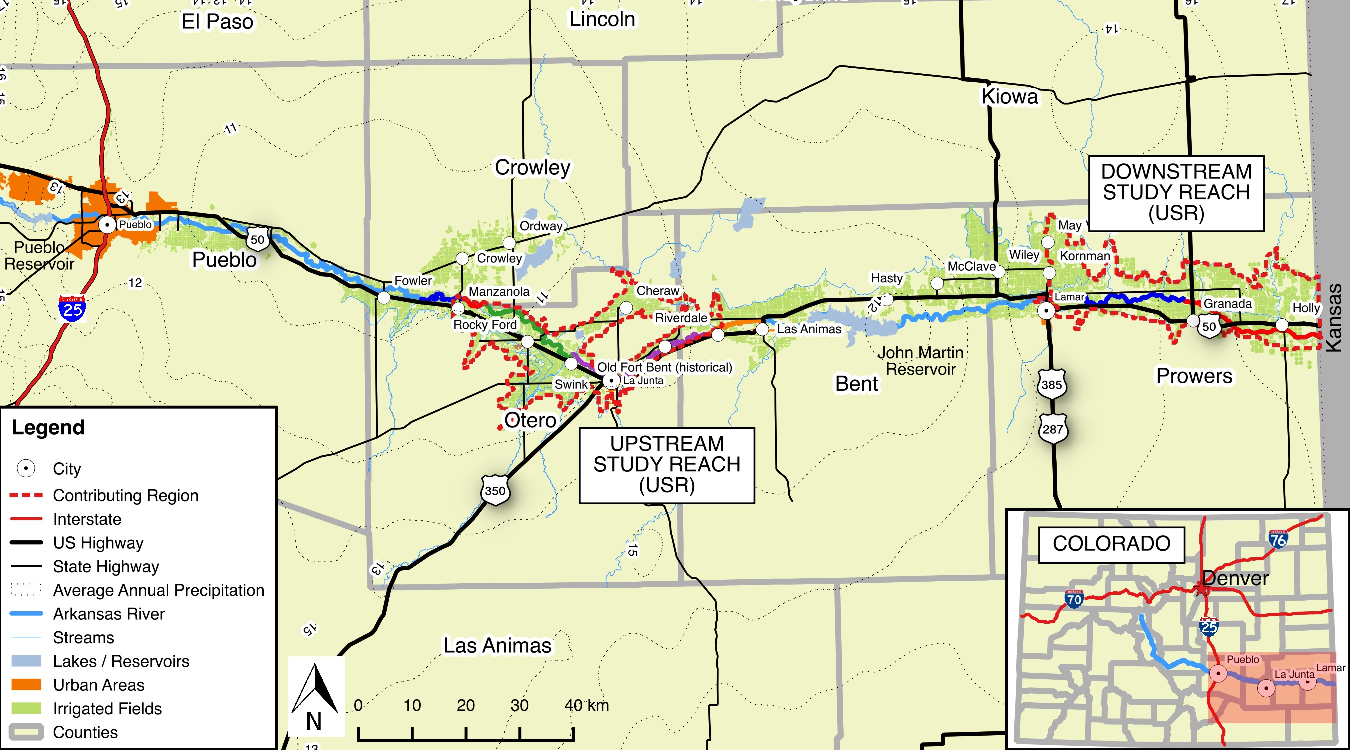
\includegraphics[width=9in]{Figures/Map/LARVRainfall}
			\caption[Precipitation in the LARV]{Precipitation in the LARV.  Values on the isolines are reported as inches of average annual rainfall.}
			\label{map:LARVRainfall}
		\end{figure}
	\end{landscape}
}

\subsection*{Anthropogenic Factors for the LARB Study Regions.}

Historically, prior to the advent of irrigated agriculture in the Ark River Basin during the 19th century, groundwater recharge in the basin occurred primarily from infiltration of precipitation through the unsaturated zone and from infiltration of surface water from losing streams.  By mid-1880s, the waters of the Arkansas R. and its tributaries were fully appropriated for normal or average years \parencite{Abbott1985}.  In areas where surface water was diverted for irrigation, infiltration of irrigation water from canals and fields became a primary source of groundwater recharge.  Natural recharge is about 0.08 inches/year in the southeast corner of the state \parencite{Wolock2003}.

The LARV river-aquifer system supplies water to towns and industries through shallow aquifer wells.  Water is returned either directly to the river after treatment or into the aquifer through groundwater seepage from treatment lagoons.  Water supplied to these entites is a very small portion when compared to the demand from agriculture in the valley.

Agriculture is the primary industry in the LARV with approx 270,00 acres irrigated \parencite{Bailey2015,Miller2010}.  There are 25 main irrigation canals in the LARV with diversion structures crossing the river.  Many fields near the river drain excess irrigation water directly back to the river \parencite{Bailey2012,Morway2013}.  There are also about 2,400 groundwater pumping wells that tap into the riparian aquifer, thereby taking water, albeit indirectly, from the river.  The floodplain is characterized by heavy agriculture on fertile soils.  The region is known for a wide variety of crops including but not limited to alfalfa, corn, grass hay, wheat, sorghum, dry beans, cantaloupe, watermelon, and onions in order of cropped area (USDA NASS Colorado Field Office 2009).  There are also a few diaries and cattle feed lots.  Most fields are irrigated using surface-irrigation methods with less than about 5\% irrigated with sprinklers or drip lines.  Surface and sprinkler irrigation efficiencies are varied depending on the crop and location \parencite{Bailey2012Phd} ref{Gates et al 2015}

Precipitation in the LARV is substantially insufficient to support crop production by about \SI{0.9}{\meter} (\SI{3}{\foot}).  It has been estimated that appropriated water rights in the LARV exceede the annual native river flow by as much as 40\% in a low flow year \parencite{cain1985,sutherland1988}.  Additional water is provided by releases from Pueblo and John Martin Reservoirs which store water during the winter period.  Some of this water is provided through trans-basin transfers through the Fryingpan-Arkansas Project.

Seepage from canals contributes significantly to the water quantity and quality in LARV aquifer.  Canals are constructed at higher elevations, promoting the surface transport of water over long distances to fields.  This elevation difference also places a higher hydraulic gradient between the canal and aquifer.  Canals, as a rule, are not constructed such that groundwater infiltrates into the canal channel.  The entire process promotes the movement of water and dissolved constituents, including \nitrate, Se, U, and salts directly into the aquifer.  Additionally, a significantly large quantity of the total canal length in the LARV is located away from the river.  This has two results.  Since the aquifer is receiveing recharge water from the canals, it acts as a reservoir, delaying the return of that water to the river channel.  This result is seen during low flow conditions when the river channel still contains water, even though historic conditions would tell us otherwise.  The second result is that dissolved constituents are introduced into the aquifer where it is the shallowest, along the edges of the valley.  This brings \nitrate and dissolved oxygen into contact with the Se bearing bedrock before either can be siginficantly depleted through other redox reactions \parencite{Bailey2012Phd,Morway2013}.

%\todo{--  Paragraph describing how irrigation and flows from canal seepage induce high concentrations of salt, Se, U, and nutrients throug evapo-transpiration and dissolution processes.  Tell how do these solutes travel to the stream system driven by the large groundwater gradients .}

%\todo{-- Briefly describe the distinctions between the geologic sources of Se (Ref: Gates et al 2009) and irrigation practices in the regions feeding the USR and DSR (Ref: Gates et al 2012, 2015) that would influence return flows and Se loading along these reaches. --}


\clearpage{}
\section{Upstream Study Reach and Surrounding Region}
\label{sec:upstream study region and river reach}
The upstream boundary of the USR starts immediately downstream of the Catlin Canal diversion dam.  The dam is approximately 4.5 miles (mi) (7 km) west of the intersection of U.S. Highway 50 and State Highway 207 in Manzanola and 4.5 mi (7 km) east of the intersection of U.S. Highway 50 and State Highway 164 in Fowler.  The USR extends along approximately 61.5 mi (99 km) of the river to where U.S. Highway 50 crosses the Arkansas River north of Las Animas.  All portions of the USR are in CDWR Division 2, Water District 17 which extends from Fowler to Las Animas.  There are three main tributaries, multiple minor tributaries, five main irrigation canals, and one return canal (for augmentation flow) are present in the USR.  Figure \ref{fig:USR map} shows the extent and approximate path of the USR and the irrigated region supplyiing return flow to the reach.

\afterpage{%
	\clearpage%
	\begin{landscape}
	\begin{figure}
		\centering
		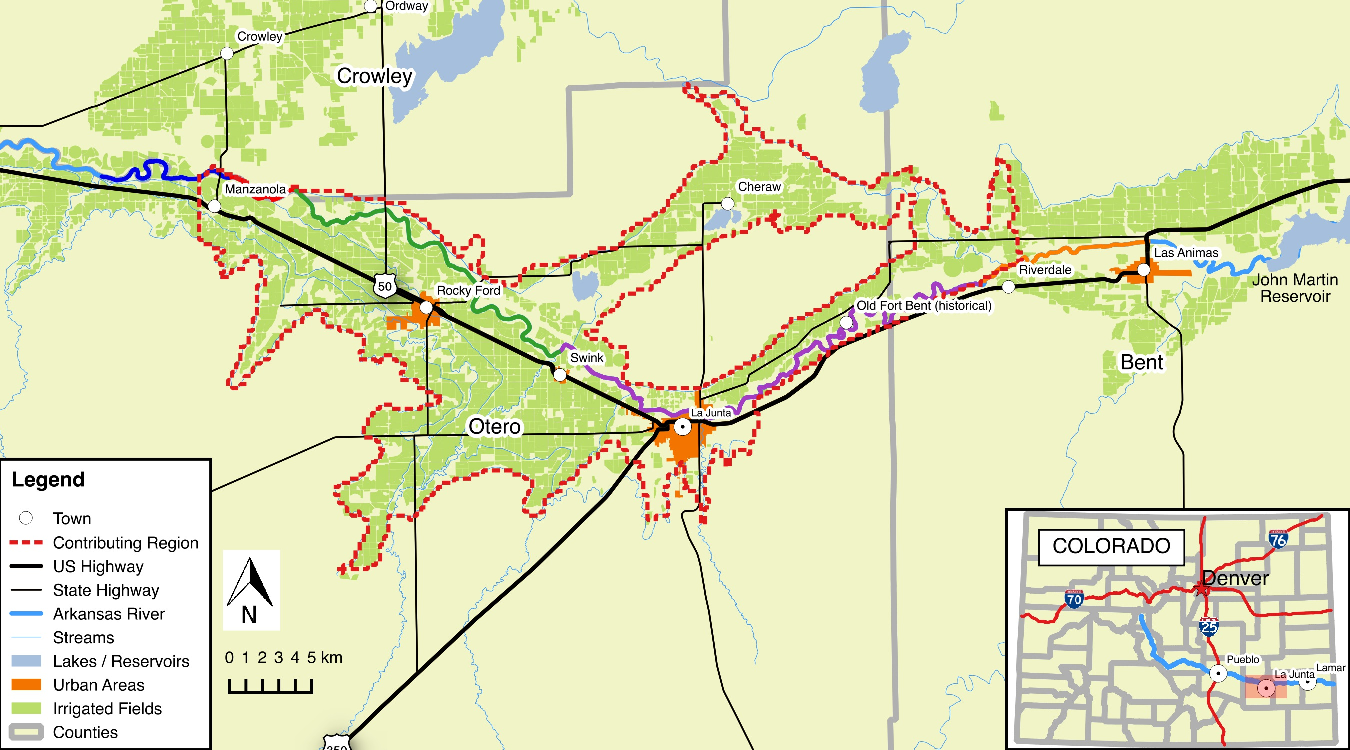
\includegraphics[width=9in]{Figures/Map/USR}
		\caption[Upstream Study Reach.]{Upstream Study Reach.  River segments within the USR are color coded.}
		\label{fig:USR map}
	\end{figure}
	\end{landscape}
}

The USR is separated into five segments given designations from "A" to "E" (Figure \ref{fig:USR map}).  Segments are geographically separated by irrigation canal diversion dams.  Segment B is the only segment that does not contain a stream gauge on the main stem of the river.  It is relatively short and has an additional diversion dam within its boundary.  Typically, significantly different flows pass through the main channel of the river within each segment.  Segments were defined to provide boundaries for river storage volume calculations.  Within each segment, except for segment B, the water surface level is determined primarily by flowrate, hydraulic geometry, and hydraulic resistance.  Knowledge of the water surface level is necessary for estimating the river storage volume.  A discussion of the river geometry analysis and storage volume calculation is provided in sections \ref{sec:River Survey} and \ref{sec:River Volume Change}. 

Figure \ref{fig:USR line map} is a line diagram representing the major flow paths in the USR.  This diagram is not to scale and depicts only the major canals and tributaries.  The segments within the reach are color coded.  Four canal diversion dams separate the segments.  Points in Figure \ref{fig:USR line map} designated as "Water Quality" are locations where CSU field technicians routinely took water samples for analysis.  A discussion of the sampling and analysis methods is presented in section \ref{sec:field data collection}.

\afterpage{%
	\clearpage%
	\begin{landscape}
	\begin{figure}
	\centering
		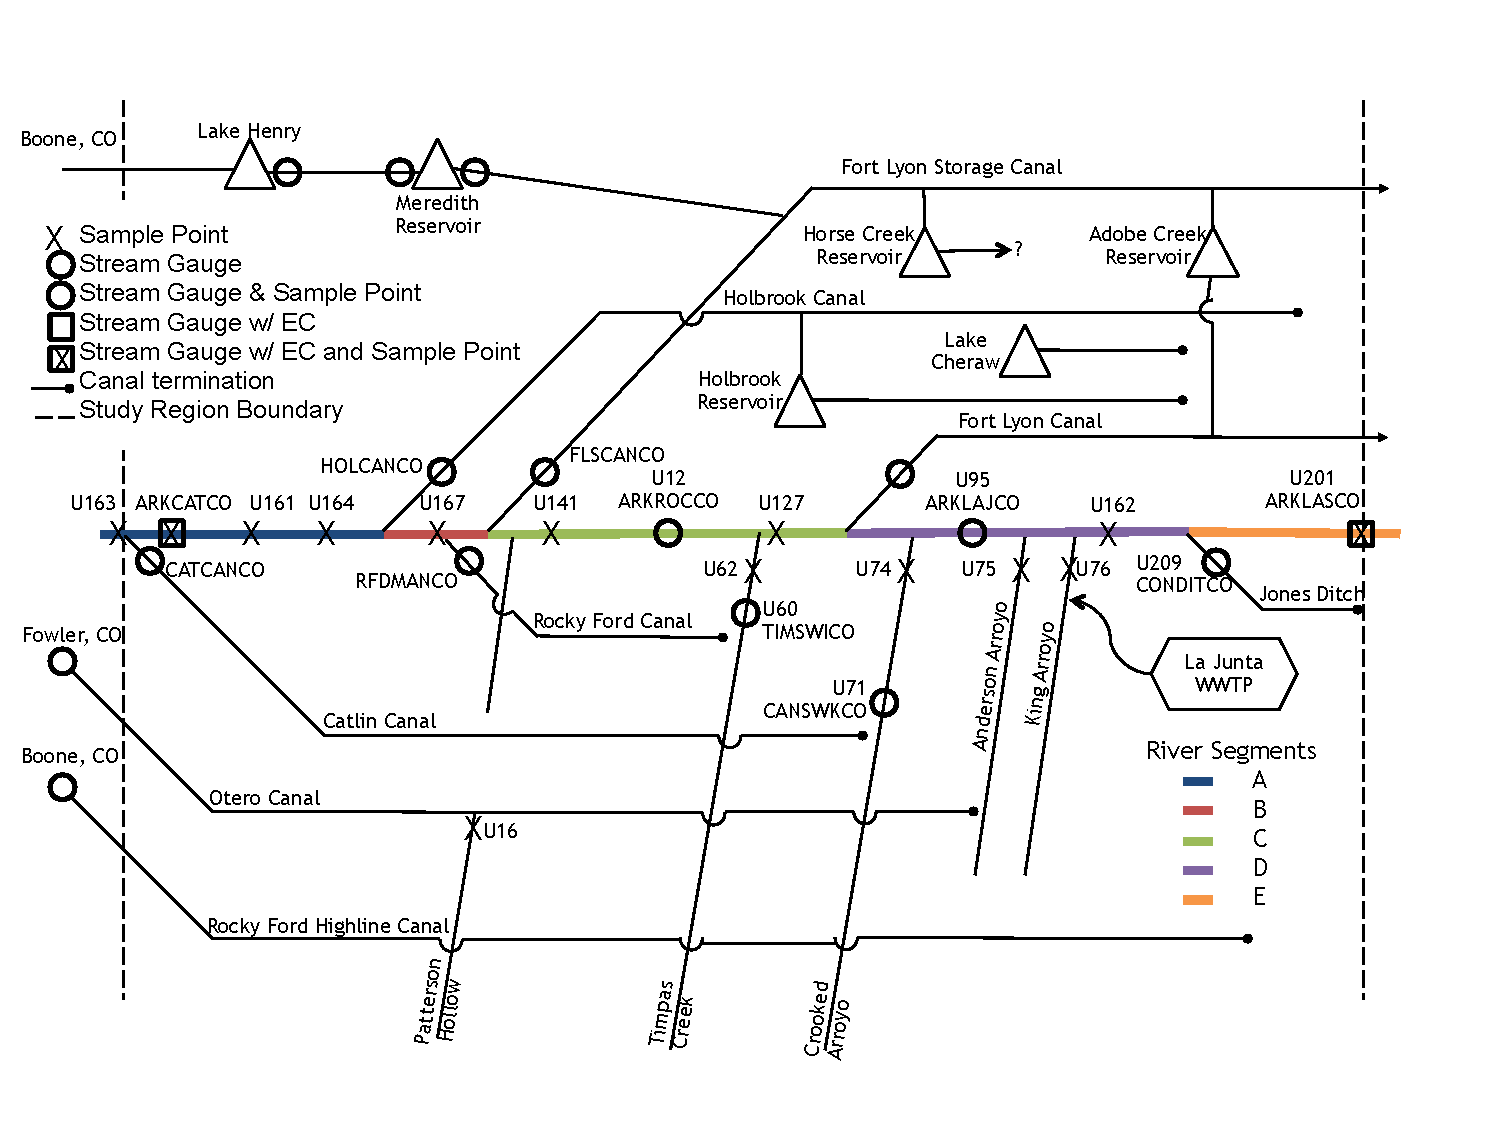
\includegraphics[width=9in]{Figures/LineDiagram/USRLineDiagram}
		\caption[Upstream Study Reach Flow Diagram.]{Upstream Study Reach Flow Diagram.}
		\label{fig:USR line map}
	\end{figure}
	\end{landscape}
}

The main tributaries are perennial and supply water to the Arkansas River under most conditions.  These tributaries are Timpas Creek, Crooked Arroyo, and Horse Creek.  Most of the minor tributaries are usually dry and only convey water during larger rainfall events and flood conditions.  All three major tributaries have a significant portion of their flows provided by agricultural runoff.

There are two minor tributaries that provide low volume, perennial flows to the Arkansas River: King Arroyo and Anderson Arroyo.  King Arroyo is assumed to be primarily fed by La Junta Waste Water Treatment Plant (WWTP) effluent.  The La Junta Water Treatment Plant (WTP) effluent spills into Anderson Arroyo.  It is currently unknown what groundwater and other flows contribute to the discharge from King or Anderson Arroyos.  No discharge data are provided for the La Junta WTP due to the very low discharge rates.  The discharge from the La Junta WWTP is included in the models.  

Patterson Hollow, a poorly-defined natural drainage, is depicted on the line graph as connected to the Arkansas River.  Flows from the upper reach of Patterson Hollow are diverted to the Otero Canal.  The reasons for the diversion are unknown, but it is speculated that the majority of the flows upstream of Otero Canal are irrigation returns and the diversion was an attempt to re-use valuable irrigation water.  Regardless, since Patterson Hollow, for the most part, was separated from the Arkansas River, it was not included in this study.

The five major canals diverting water from the Arkansas River along the USR are Holbrook Canal, Rocky Ford Canal, Fort Lyon Storage Canal, Fort Lyon Canal, and Jones Ditch.
The Rocky Ford Return Canal is the only monitored canal returning augmentation water to the Arkansas River in the USR.  
The Rocky Ford Return Canal diverts water from the Rocky Ford Canal and returns it directly to the Arkansas River. 
This system is in place to monitor and augment flows in conjunction with trans-basin flows used by the City of Aurora.  
The Otero and Rocky Ford Highline Canals run parallel to the USR.  They divert water from the Arkansas River upstream of the USR upstream boundary.  
Overflows from these two canals pass through the tributary gauge in Crooked Arroyo.

\clearpage{}
\section{Downstream Study Reach and Surrounding Region}
\label{sec:downstream study region and river reach}

The DSR begins at the U.S. Highway 50/U.S. Highway 287 Arkansas River crossing in Lamar, Colorado, and extends approximately 71 km to the Colorado/Kansas state line (Figure \ref{fig:DSR map}).  Figure \ref{fig:DSR line map} is a line diagram representing the flow structure within the DSR.  Similar symbology is used on these maps as in Figures \ref{fig:USR map} and \ref{fig:USR line map} for the USR.  For a period of time, there were four tributaries and drains in the DSR where flows were measured mannually gauged on an infrequent basis.  The results of the this stream gauging activity do not affect the calculation or analysis of this study, but will be discussed in the conclusion.  The entirety of the DSR lies within CDWR Division 2, District 67 and contains two major tributaries, multiple minor tributaries, and one irrigation canal. 

\afterpage{%
	\clearpage%	
	\begin{landscape}
	\begin{figure}%[htbp]
		\centering
		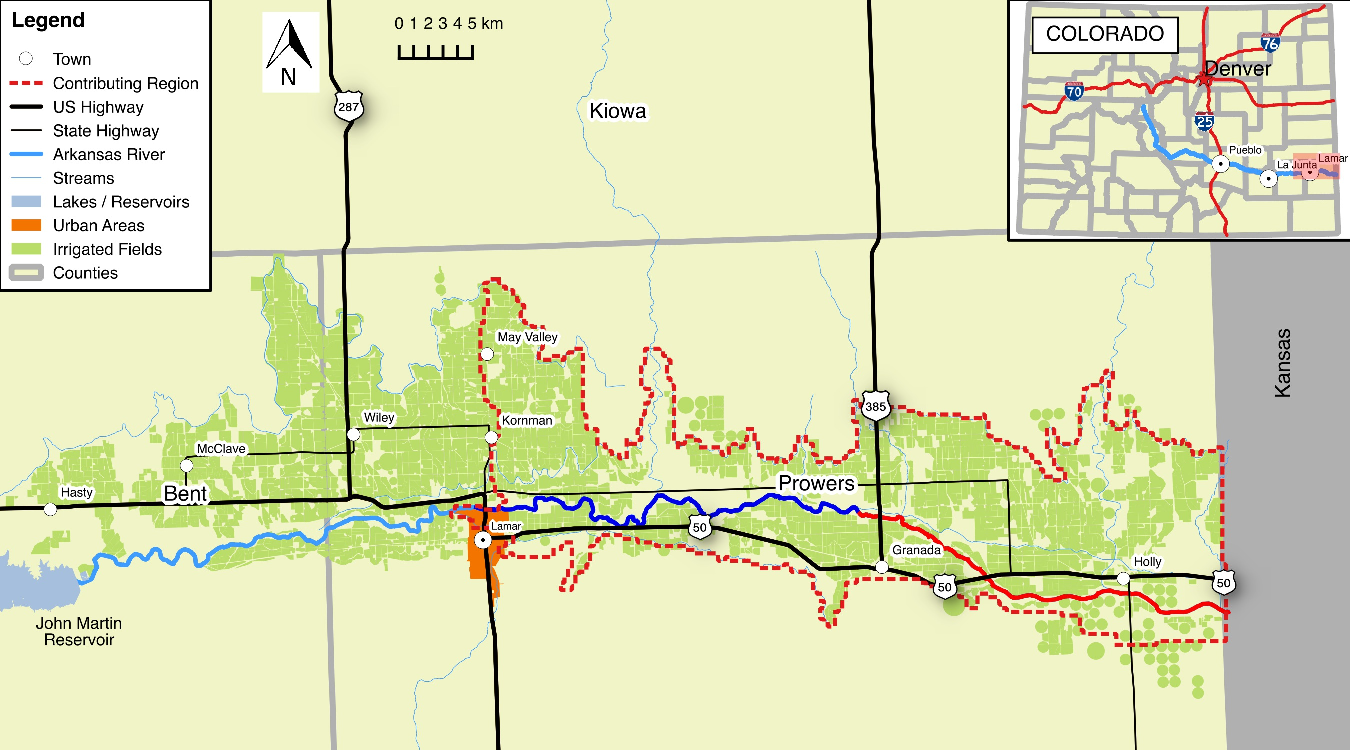
\includegraphics[width=9in]{Figures/Map/DSR}
		\caption[Downstream Study Reach.]{Downstream Study Reach.  River segments within the DSR are color coded.}
		\label{fig:DSR map}
	\end{figure}
	\end{landscape}
}

\afterpage{%
	\clearpage%
	\begin{landscape}
	\begin{figure}
		\centering
			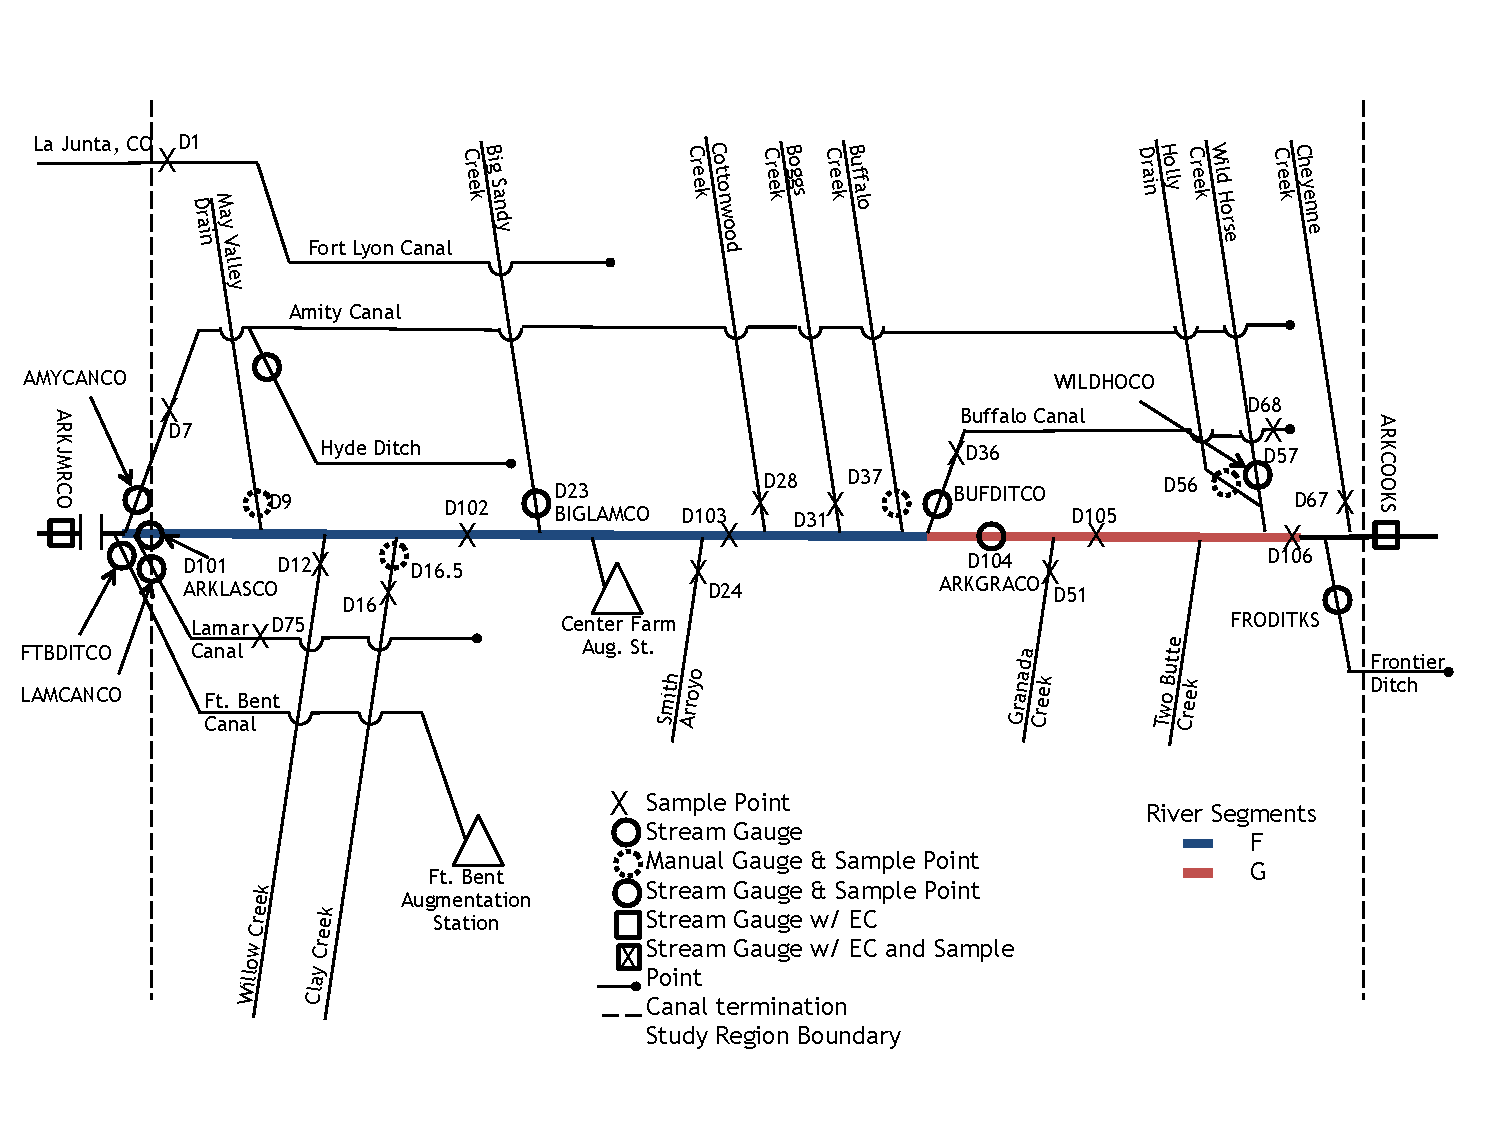
\includegraphics[width=9in]{Figures/LineDiagram/DSRLineDiagram}
			\caption[Downstream Study Reach Flow Diagram.]{Downstream Study Reach Flow Diagram.}
			\label{fig:DSR line map}
	\end{figure}
	\end{landscape}
}

The DSR is separated into Segment F and Segment G as shown in figure \ref{fig:DSR map}. The diversion dam for the Buffalo Ditch irrigation canal is the boundary between the two DSR segments.  Field technicians have observed complete diversion of the Arkansas River at the Buffalo Ditch diversion with small but significant flows reappearing in the Arkansas River channel only a few kilometers downstream.  This leads to the speculation that significant portions of the downstream in-channel flow are from groundwater return flow.

The major tributaries within the DSR are Big Sandy Creek and Wild Horse Creek.  CSU field technicians have observed that the stream gauge on Big Sandy Creek has been affected by beaver dams constructed downstream of the gauge and upstream of the culvert passing under State Highway 196.  The stream gauge on Wild Horse Creek is operated seasonally from April through November.  CSU has made many visual flow observations in these creeks outside of the irrigation season.  The off season flows are either extremely low or the stream is frozen.

Unlike the USR, most of the minor tributaries in the DSR flow most of the year except in drought conditions.  The primary source of water in the minor tributaries is irrigation runoff flowing into the streams through surface and subsurface flow paths.  Most minor tributaries in the DSR do not have definitive entry points to the Arkansas River channel resulting in doubt as to whether these flows reach the Arkansas River as surface water.  It was assumed herein that the minor tributary flows enter the main stem primarily as groundwater.  Minor surface return flows that do reach the Arkansas River are not gauged and most are difficult to access. 

Buffalo Canal is the only functioning canal diversion within the DSR.  There is historical and aerial imagery evidence for another diversion, but the Arkansas River has been routed around the structure and neither the CDWR nor the USGS maintain a flow gauge for the canal serviced by the diversion.

\end{linenumbers}
\clearpage{}
%% comment out the first line before production.

\renewcommand{\thechapter}{3}
\chapter{Data Collection and Compilation}
\label{chap:data collection}

\begin{linenumbers}
\section{Water Quality Data Collection}
\label{sec:field data collection}

From June 2006 to July 2011 and April 2003 to August 2011, water quality samples were taken by CSU field personnel from the Arkansas River, tributaries, and drains in the USR and DSR, respectively.   During the Se study periods, 18 surface water sampling trips were made to the USR and 46 trips were made to the DSR.  A total of 288 dissolved Se samples were taken and analyzed for dissolved Se and specific ions in the USR and 1,030 in the DSR during their respective study periods.  Table \ref{tab:SampleSummary} is a summary of the sample trips, the month and year of the trip, and the number of Se samples taken from the respective locations.  Figures \ref{map:USRSample} and \ref{map:DSRSample} show the dissolved Se sample locations in the USR and DSR, respectively.  Tables \ref{tab:USRSampleLoc} and \ref{tab:DSRSampleLoc} list the sample locations and their location with the river reach and segment.  The location of the sample point within the segment is only listed for samples collected on the Arkansas River with respect to the location of the stream gauge within the river segment.  Sample points on tributaries and drains as noted in the tables.

% Table - sample trips
\afterpage{%
	\clearpage%
	\renewcommand{\arraystretch}{0.513}
	\begin{longtable}{c C{1.25in} C{.9in} C{1in} C{.9in} C{1in}}
		\caption[Summary of USR and DSR Water Sample Events.]{Summary of USR and DSR Water Sample Events.}    \label{tab:SampleSummary} \\
			\toprule
    	Trip & \multirow{2}[1]{*}{Date} & \multicolumn{2}{c}{USR Se Samples} & \multicolumn{2}{c}{DSR Se Samples} \\\cmidrule(r{.5em}l){3-4} \cmidrule(r{.5em}l){5-6}
    	\# &  & River & Trib. \& Drain & River & Trib. \& Drain \\
    		\toprule
    	\endfirsthead
    	\caption[]{Summary of USR and DSR Water Sample Events.  (Continued)}\\
    		\toprule
    	Trip & \multirow{2}{*}{Date} & \multicolumn{2}{c}{USR Se Samples} & \multicolumn{2}{c}{DSR Se Samples} \\
    	\# &  & River & Trib. \& Drain & River & Trib. \& Drain \\
    		\toprule
    	\endhead
    		\bottomrule
    	\endfoot 
		1 & April 2003 &  &  & 12 & 14 \\
		2 & June 2003 &  &  & 12 & 15 \\
		3 & July 2003 &  &  & 7 & 15 \\
		4 & July 2003 &  &  & 6 & 16 \\
		5 & October 2003 &  &  & 6 & 15 \\
		6 & January 2004 &  &  & 6 & 15 \\
		7 & March 2004 &  &  & 6 & 15 \\
		8 & May 2004 &  &  & 6 & 15 \\
		9 & June 2004 &  &  & 6 & 15 \\
		10 & July 2004 &  &  & 6 & 15 \\
		11 & August 2004 &  &  & 6 & 15 \\
		12 & November 2004 &  &  & 6 & 17 \\
		13 & January 2005 &  &  & 6 & 15 \\
		14 & March 2005 &  &  & 6 & 15 \\
		15 & June 2005 &  &  & 6 & 17 \\
		16 & July 2005 &  &  & 6 & 15 \\
		17 & August 2005 &  &  & 6 & 17 \\
		18 & December 2005 &  &  & 6 & 16 \\
		19 & January 2006 &  &  & 6 & 16 \\
		20 & March 2006 &  &  & 6 & 16 \\
		21 & May 2006 &  &  & 6 & 16 \\
		22 & June 2006 & 10 & 5 & 6 & 16 \\
		23 & July 2006 &  &  & 6 & 16 \\
		24 & August 2006 &  &  & 6 & 16 \\
		25 & November 2006 &  &  & 6 & 16 \\
		26 & March 2007 &  &  & 6 & 16 \\
		27 & May 2007 & 10 & 5 & 6 & 16 \\
		28 & June 2007 &  &  & 6 & 16 \\
		29 & July 2007 &  &  & 6 & 16 \\
		30 & August 2007 &  &  & 6 & 16 \\
		31 & October 2007 & 10 & 4 &  &  \\
		32 & November 2007 &  &  & 6 & 16 \\
		33 & January 2008 &  &  & 6 & 16 \\
		34 & March 2008 & 10 & 4 &  &  \\
		35 & May 2008 &  &  & 6 & 16 \\
		36 & June 2008 & 10 & 5 &  &  \\
		37 & July 2008 &  &  & 6 & 16 \\
		38 & August 2008 & 10 & 5 &  &  \\
		39 & November 2008 &  &  & 6 & 16 \\
		40 & January 2009 & 10 & 5 &  &  \\
		41 & (No Se Samples) &  &  &  &  \\
		42 & March 2009 &  &  & 6 & 16 \\
		43 & May 2009 & 10 & 5 &  &  \\
		44 & June 2009 &  &  & 6 & 16 \\
		45 & July 2009 & 10 & 4 &  &  \\
		46 & August 2009 &  &  & 6 & 16 \\
		47 & November 2009 & 10 & 4 &  &  \\
		48 & January 2010 &  &  & 6 & 16 \\
		49 & March 2010 & 10 & 4 & 6 & 15 \\
		50 & May 2010 & 9 & 4 &  &  \\
		51 & June 2010 &  &  & 6 & 16 \\
		52 & July 2010 & 11 & 6 &  &  \\
		53 & August 2010 & 10 & 7 & 6 & 17 \\
		54 & November 2010 & 12 & 7 & 8 & 19 \\
		55 & March 2011 & 12 & 7 & 8 & 19 \\
		56 & May 2011 & 15 & 9 & 8 & 17 \\
		57 & July 2011 & 12 & 7 &  &  \\
		58 & August 2011 &  &  & 8 & 17 \\\cmidrule{3-6}\morecmidrules\cmidrule{3-6}
		& Totals & 191 & 97 & 297 & 733\\
	\end{longtable}%
	\renewcommand{\arraystretch}{1.95}
}

% Map - USR sample locations
\afterpage{%
\clearpage%
	\begin{landscape}
	\begin{figure}
		\centering
		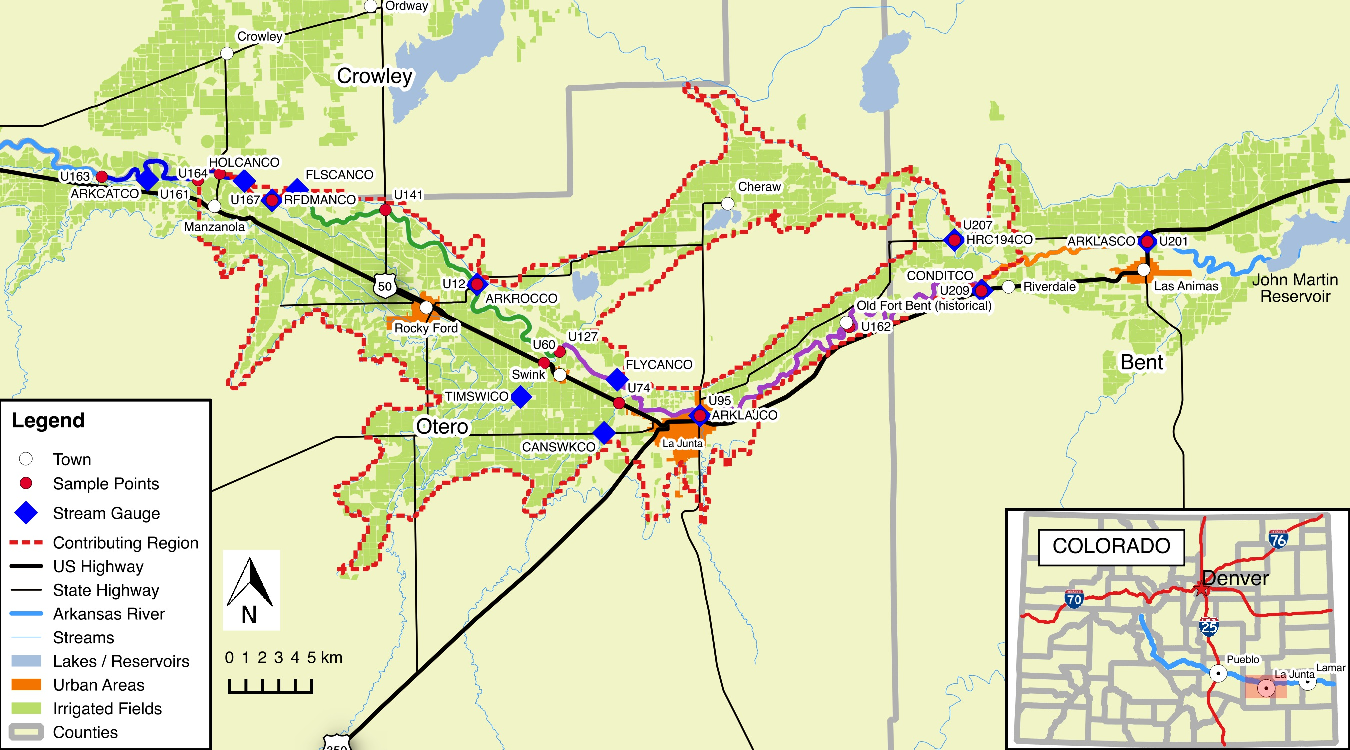
\includegraphics[scale=1]{Figures/Map/USRSample}
		\caption[Dissolved Se sampling locations in the USR.]{Dissolved Se sampling locations in the USR.  Samples taken near, but not at stream gauge locations where shown.}
		\label{map:USRSample}
	\end{figure}
	\end{landscape}	
}

% Map - DSR sample locations
\afterpage{%
\clearpage%
	\begin{landscape}
	\begin{figure}
		\centering
		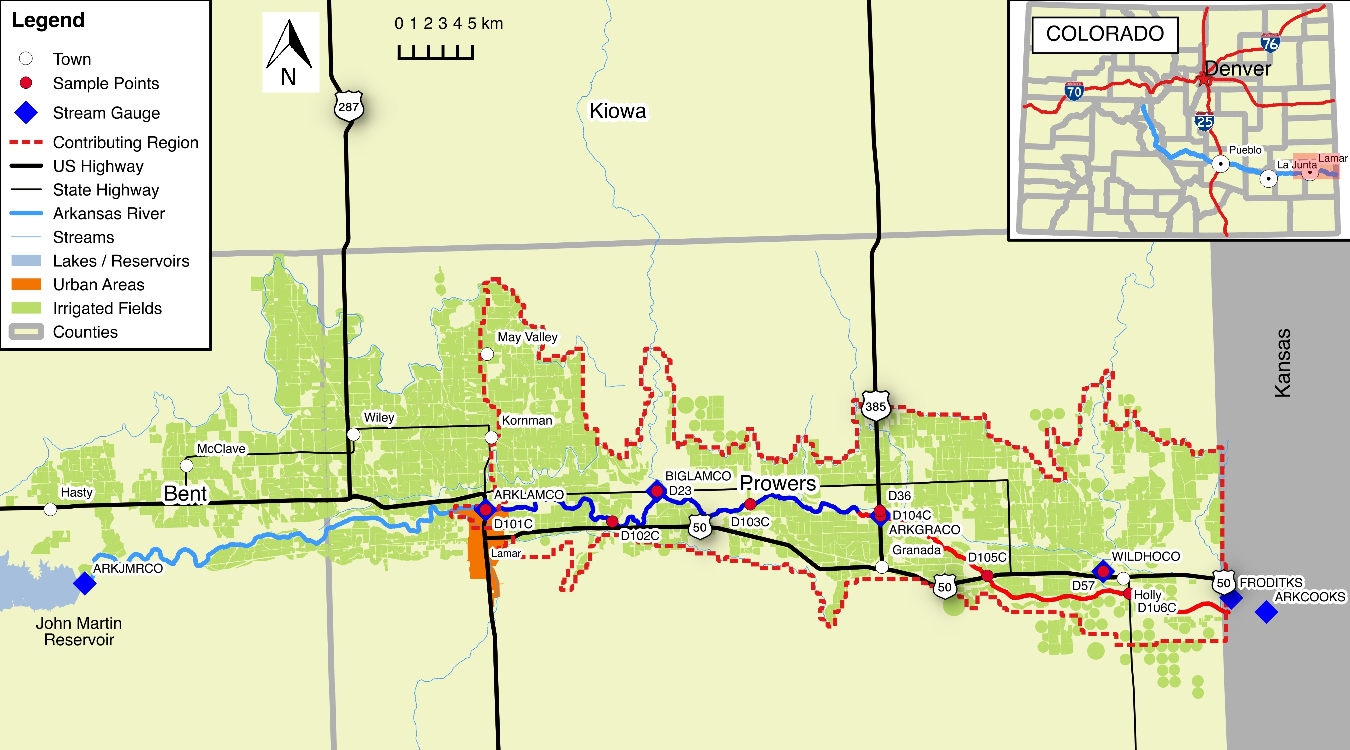
\includegraphics[scale=1]{Figures/Map/DSRSample}
		\caption[Dissolved Se sampling locations in the DSR.]{Dissolved Se sampling locations in the DSR.  Samples taken near, but not at stream gauge locations where shown.}
		\label{map:DSRSample}
	\end{figure}
	\end{landscape}	
}

% Table - USR sample locations
\begin{table}[htbp]
	\centering
	\caption[Upstream Study Region (USR) Sample Collection Point Information.]{Upstream Study Region (USR) Sample Collection Point Information.  A value of zero (0) indicates the location of the segment stream gauge.  Negative distances indicate the point is upstream of the reference stream gauge location. Segment B does not contain a stream gauge on the river main stem.}
	\label{tab:USRSampleLoc}
	\begin{tabular}{cccccc}
		\toprule
		River                       & Sample &  \multicolumn{2}{c}{Dist from}   &   \multicolumn{2}{c}{Dist from}   \\
		Segment                      & Point  & \multicolumn{2}{c}{USR Upstream} & \multicolumn{2}{c}{River Segment} \\
		Name                        &        &   \multicolumn{2}{c}{Boundary}   & \multicolumn{2}{c}{Stream Gauge}  \\
		\cmidrule(r{.5em}l){3-4} \cmidrule(r{.5em}l){5-6} &        &  mi  &            km             &  mi  &             km             \\ \toprule
		\multirow{3}{*}{A}                 &  U163  &  0   &             0             & -2.7 &            -4.3            \\
		&  U161  & 5.8  &            9.3            & 3.1  &             5              \\
		&  U164  & 6.8  &           10.9            & 4.1  &            6.6             \\ \midrule
		B                         &  U167  & 9.2  &           14.8            &      &  \\ \midrule
		\multirow{4}{*}{C}                 &  U141  & 14.7 &           23.7            & -5.5 &            -8.9            \\
		&  U12   & 20.2 &           32.5            &  0   &             0              \\
		&  U60   & 26.1 &            42             & 5.9  &            9.5             \\
		&  U127  & 26.4 &           42.5            & 6.2  &             10             \\ \midrule
		\multirow{4}{*}{D}                 &  U74   & 30.3 &           48.8            & -3.5 &            5.6             \\
		&  U95   & 33.8 &           54.4            &  0   &             0              \\
		&  U162  &  44  &           70.8            & 10.2 &            16.4            \\
		&  U209  & 52.8 &            85             &  19  &            30.6            \\ \midrule
		\multirow{2}{*}{E}                 &  U207  & 55.1 &           88.7            & -6.6 &           -10.6            \\
		&  U201  & 61.7 &           99.3            &  0   &             0              \\ \bottomrule
	\end{tabular}
\end{table}

% Table - DSR sample locations
\begin{table}[htbp]
	\centering
	\caption[Downstream Study Region (DSR) Se Sample Location Information.]{Downstream Study Region (DSR) Se Sample Location Information.  A value of zero (0) indicates the location of the segment stream gauge.  Negative distances indicate the point is upstream of the reference stream gauge location.}
	\label{tab:DSRSampleLoc}
	\begin{tabular}{cccccc}
		\toprule
		River                        & Sample &  \multicolumn{2}{c}{Dist from}   &   \multicolumn{2}{c}{Dist from}   \\
		Segment                       & Point  & \multicolumn{2}{c}{USR Upstream} & \multicolumn{2}{c}{River Segment} \\
		Name                         &        &   \multicolumn{2}{c}{Boundary}   & \multicolumn{2}{c}{Stream Gauge}  \\
		\cmidrule(r{0.5em}l){3-4} \cmidrule(r{0.5em}l){5-6} &        &  mi  &            km             &  mi  &             km             \\ \toprule
		\multirow{5}{*}{F}                  & D101C  &  0   &             0             &  0   &             0              \\
		& D102C  & 7.9  &           12.7            & 7.9  &            12.7            \\
		&  D23   & 11.6 &           18.7            & 11.6 &            18.7            \\
		& D103C  & 17.6 &           28.3            & 17.6 &            28.3            \\
		&  D36   & 23.4 &           37.7            & 23.4 &            37.7            \\ \midrule
		\multirow{4}{*}{G}                  & D104C  & 24.9 &           40.1            &  0   &             0              \\
		& D105C  & 31.2 &           50.2            & 6.3  &            10.1            \\
		&  D57   & 38.1 &           61.3            & 13.2 &            21.2            \\
		& D106C  & 38.9 &           62.6            &  14  &            22.5            \\ \bottomrule
	\end{tabular}
\end{table}

Sample collection trips involved hours of preparation.  Before leaving for the study region(s), equipment and supplies were prepared.  Peristaltic pumps were used for all surface water sample collection.  Two Durham Geo TR-200 PSP peristaltic pumps were taken on each trip.  The TR-200 is a single head, bi-directional, 12-volt battery operated, portable sampling pump capable of delivering flow rates up to \SI{500}{\milli\liter\per\minute} in both directions (Figure \ref{pic:pump}).  The pumps were cleaned, in-situ water quality instruments were calibrated, and sample collection bottles were prepared.  Peristaltic pumps were cleaned at the beginning and end of each sampling day and before sampling at each field sampling location.  Figure \ref{pic:SampleVehicle} is a picture of a typical vehicle setup with cleaning buckets, peristaltic pump, water quality sonde, and various other equipment items.  Cleaning consisted of the following listed procedure:% listed in table xx.

\clearpage%
% List - sample cleaning procedures
\begin{enumerate}
	\item At the beginning of every sampling day, four, 5-gallon (gal) buckets with lids were prepared as follows:
	\begin{enumerate}
		\item One bucket filled with approximately \SI{2.5}{\gallon} tap water and approximately \SI{20}{\milli\liter} of lab grade hydrochloric acid (HCl).
		\item One bucket filled with approximately \SI{2.5}{\gallon} tap water and approximately \SI{20}{\milli\liter} of LiquiNox\textregistered, a lab grade, phosphate and ammonia free, free rinsing detergent.
		\item Two buckets filled with approximately \SI{2.5}{\gallon} deionized water.
	\end{enumerate}
	\item The acid solution was run through the pump for two minutes.  This disinfected the pump tubing and prevented cross contamination.
	\item The detergent solution was run through the pump for two minutes.  This removed any remaining soil particles from the pump tubing.
	\item Water from the first of the deionized water buckets was run through the pump for two minutes followed water from by the second bucket of deionized water for another two minutes.  This rinsed all detergent from the pump tubing.
\end{enumerate}

% Picture - peristaltic pump and YSI
\begin{figure}[htbp]
	\centering
	\subcaptionbox{Durham Geo TR-200 PSP Peristaltic Pump.\label{pic:pump}}{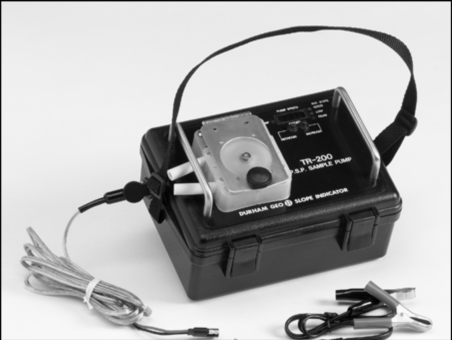
\includegraphics[width=2.5in]{Figures/Photo/PeristalticPump}}\hspace{4em}%
	\subcaptionbox{In Situ Water Quality Sonde and Data Logger.  Measures temperature, specific conductivity, pH, oxidation-reduction potential, and dissolved oxygen concentration.\label{pic:ysi}}{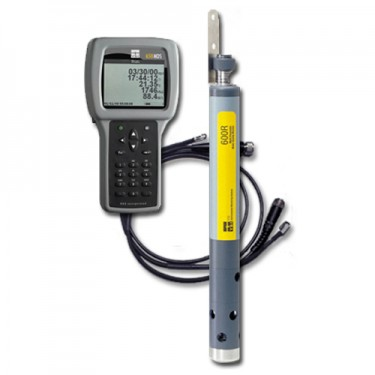
\includegraphics[width=2.5in]{Figures/Photo/ysi}}
	\caption[Water Quality Sampling Equipment.]{Water Quality Sampling Equipment.}
	\label{fig:WQEquipment}
\end{figure}

% Picture - Pickup truck set-up for sampling.
\begin{figure}
	\centering
	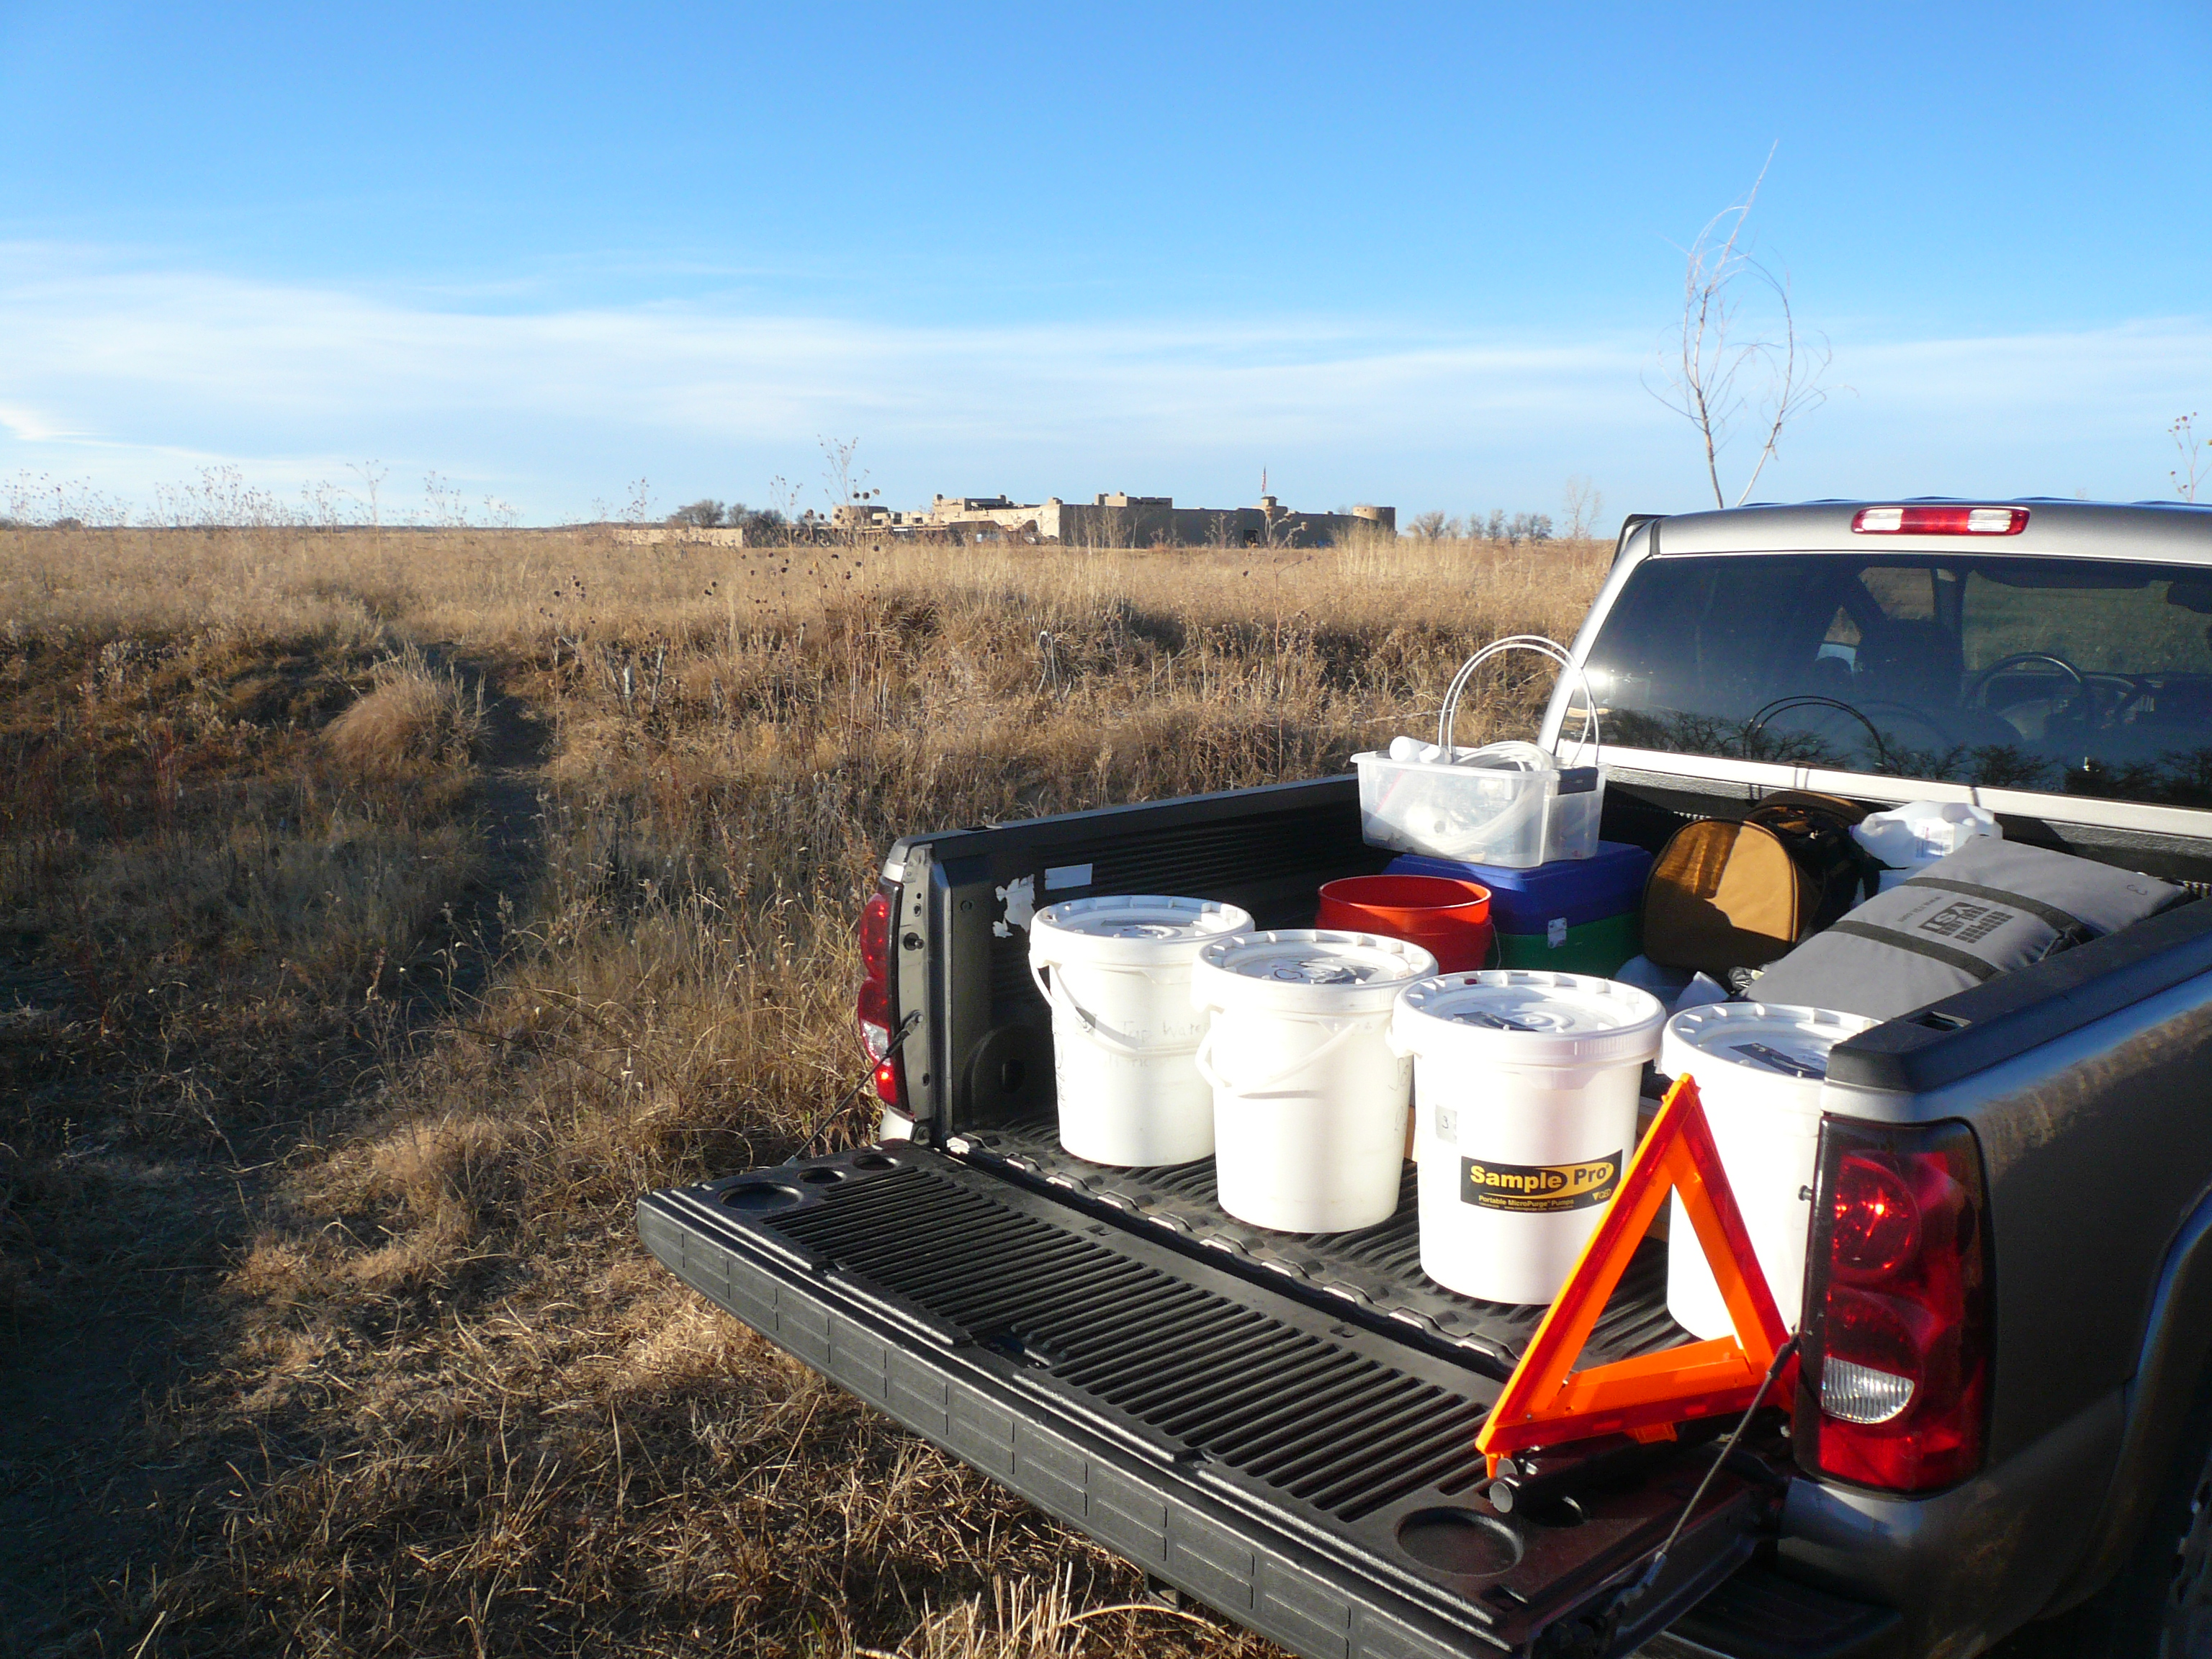
\includegraphics[width=4in]{Figures/Photo/SampleVehicle}
	\caption[Typical sample vehicle equipped for surface water sampling.]{Typical sample vehicle equipped for surface water sampling.  Equipment includes peristaltic pump, water quality sonde, pump cleaning buckets, and various other equipment items.  This picture is taken at sample site U162 which is on the National Park Service's Bent's Old Fort National Historic Site (fort in background).}
	\label{pic:SampleVehicle}
\end{figure}	

Two sample types were routinely taken at all locations during each trip.  One sample type was for the analysis of specific ion concentrations as a general water quality panel.  A \SI{250}{\milli\liter}-wide mouth, high density poly-ethylene (HDPE) bottle was used to collect and ship the specific ion samples.  This bottle was pre-cleaned and shipped to CSU by Ward Laboratories, Inc. in Kearney, Nebraska, the laboratory that provided the bulk of the water quality analysis services.  The second sample was taken for analysis of dissolved Se concentration using a \SI{125}{\milli\liter}-wide mouth, HDPE bottle.  This bottle was procured from multiple sources and pre-cleaned to the US EPA's "Specifications and Guidance for Contaminant Free Sample Containers" \citep{EPA1992}.  Approximately \SI{0.6}{\milli\liter} of a diluted nitric acid solution prepared with \SI{33}{\milli\liter} of distilled water and \SI{7}{\milli\liter} of ultra-pure nitric acid was added to each bottle using a graduated pipette.  This was done to preserve the sample by lowering the pH to less than 2 standard pH units.  During the latter half of the sampling periods, samples for dissolved uranium (U) were gathered during most sampling trips.  \SI{250}{\milli\liter}-narrow mouth, pre-cleaned, pre-preserved with nitric acid, HDPE bottles were provided by TestAmerica Inc., the laboratory providing dissolved uranium analysis.

Blank samples of deionized water were prepared in the lab for each sample type before each trip at the beginning of each sampling day for each sample type.  Blanks are intended to be free of the analyzed constituent and are used to test the samples for bias due to contamination.  Trip blanks were taken in the lab before the begining of the sample trip.  They accompanied field personnel during all sampling activities and were then shipped to their respective lab for analysis.  Trip blanks were intended to demonstrate that there was no contamination due to transportation activities.  Field blanks were taken in the field at the begining of the sampling day.  These samples also accompanied the field personnel during sampling activities and were shipped to their respective lab for analysis.  Field blanks were intended to demonstrate that there was no contamination in the sampling equipment.   Any variation from non-detectable solute concentration in these blanks would indicate possible contamination of the water samples taken that day and further investigation would be required.  None of the lab results from field or trip blanks reported values that would indicate sample contamination.

Two YSI, Inc. 600R sondes with attached YSI, Inc. 650 MDS display data loggers were used for in-situ measurements during each sample trip (Figure \ref{pic:ysi}).  The sondes were equipped with a Rapid Pulse polarographic dissolved oxygen (DO) sensor capable of measuring DO from \SIrange{0}{50}{\milli\gram\per\liter}, \SI{\pm2}\%; a thermistor capable of measuring temperature from \SIrange{-5}{50}{\degreeCelsius}, \SI{\pm0.15}{\degreeCelsius}; a glass combination electrode pH sensor capable of measuring pH in the range of 0 to 14 units, $\pm$0.2 units; a platinum button oxidation-reduction potential (ORP) sensor capable of measuring in the range of \SIrange{-999}{999}{\milli\volt}, \SI{\pm20}{\milli\volt}; and a four electrode, autoranging  cell capable of measuring electrical conductivity (EC) as specific conductance at \SI{25}{\degreeCelsius} in the range of \SIrange{0}{100000}{\micro\siemens\per\centi\meter}, $\pm$0.5\%~+~\SI{1}{\micro\siemens\per\centi\meter}.  The equipment was serviced and calibrated by CSU field personnel before every trip to the study reaches and at the end of every sampling day.  Sondes were sent to Geotech Environmental Equipment, Inc. annually for maintenance checks.  Geotech Environmental Equipment, Inc. is an authorized dealer and service provider for YSI equipment with an office in Denver, Colorado.

At least one set of duplicate water samples was taken per sampling trip to the USR and/or DSR.  Duplicate, or replicate, samples were marked as 'A' and 'B' samples.  The 'A' sample results were kept with the main data set and were used as the primary data set.  'B' sample results were kept separate and were used to determine the combined sampling methodology and lab analysis uncertainty.  The sampling standard procedure was to take one duplicate set of surface water samples per day with a minimum of two duplicate surface water samples per sampling trip.

Each sampling event began with recording the site data on a form (log) similar to the one in Figure~\ref{fig:samplog}.  In-situ water quality measurements were then taken using the YSI sonde.  The data logger was used to read the data, but was not used as a recording device.  All data were recorded on the form shown as an example in Figure~\ref{fig:samplog}.  The ranges at the bottom of the form are maximum acceptable ranges of values determined from previous sampling trips.  Values outside of these ranges would indicate to field personnel that the equipment was damaged, had lost calibration, or operational error had occured.  The YSI sonde was allowed to rest in the water for a minimum of three minutes before recording values.  Usually, the sonde would rest in the water while water quality samples were taken.  Samples were pumped through a disposable, in-line \SI{0.45}{\micron}, polyethersulfone filter into the sample bottles.  Peristaltic pumps were used to extract all water samples from surface water sources.  No air space was permitted in any of the sample bottles.  Figure \ref{pic:samplingSub1} shows a trained sample collector at location U12 in the USR which is north of Rocky Ford on a bridge over the Arkansas River.  The YSI sonde is not in this image, but is suspended in the river during sample collection.  Figure \ref{pic:samplingSub2} is the same sample collector at sample location U73 in the USR recording readings from the YSI sonde.  Samples were stored on ice or in a refrigerator until they were shipped to their respective labs.  Data was recorded onto the data form from the YSI sonde immediately after collectiing the water samples.  The sonde was left in the water for an additional two to three minutes.  Any changes in readings were recorded as a second entry.  An example of a completed log is shown in Figure~\ref{fig:samplogComplete}

% Figure - blank sample log
\begin{figure}[htbp]
	\centering
	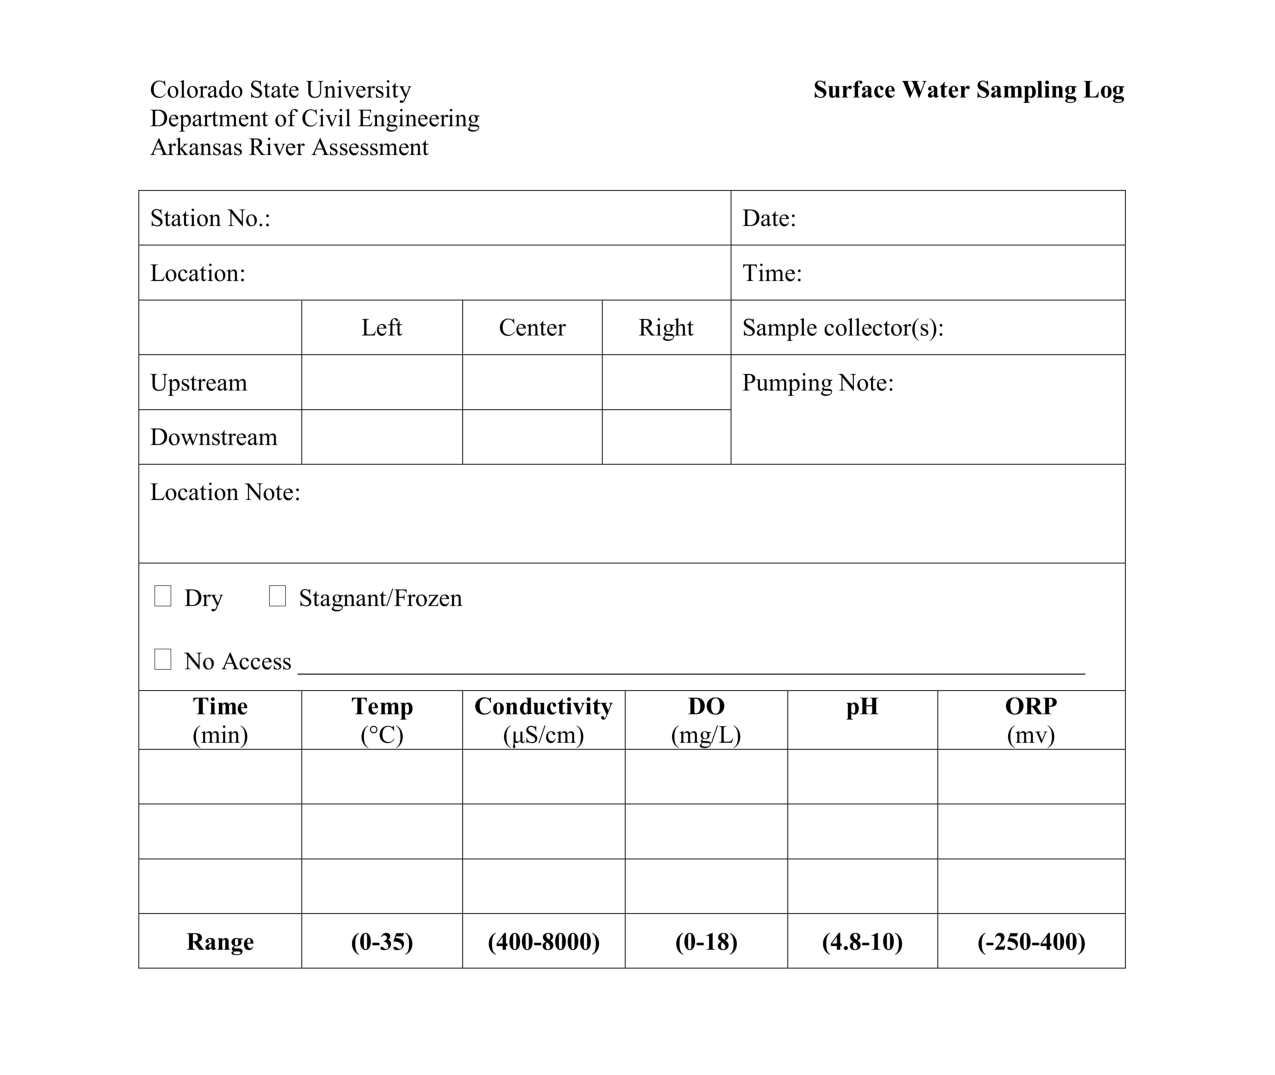
\includegraphics[width=6in]{Figures/SampleLog}
	\caption[Example water quality sample form.]{Example water quality sample form.}
	\label{fig:samplog}
\end{figure}

% Picture - samples being taken
\begin{figure}[htbp]
\centering
	\subcaptionbox{Sample location U12.  The Se sample bottle is being filled with a peristaltic pump through a \SI{0.45}{\micron} filter.  The specific ion sample bottle is filled, laying next to the pump.\label{pic:samplingSub1}}{\includegraphics[width=2.5in]{Figures/Photo/SampleFromBridge}}\hspace{4em}%
	\subcaptionbox{Sample location U73.   Personnel is hand logging data from the YSI sonde.\label{pic:samplingSub2}}{\includegraphics[width=2.5in]{Figures/Photo/SampleAtSmallTrib}}
	\caption[Personnel performing water sample collection.]{Personnel performing water sample collection.}
	\label{pic:sampling}
\end{figure}

% Figure - filled sample log
\begin{figure}[htbp]
	\centering
	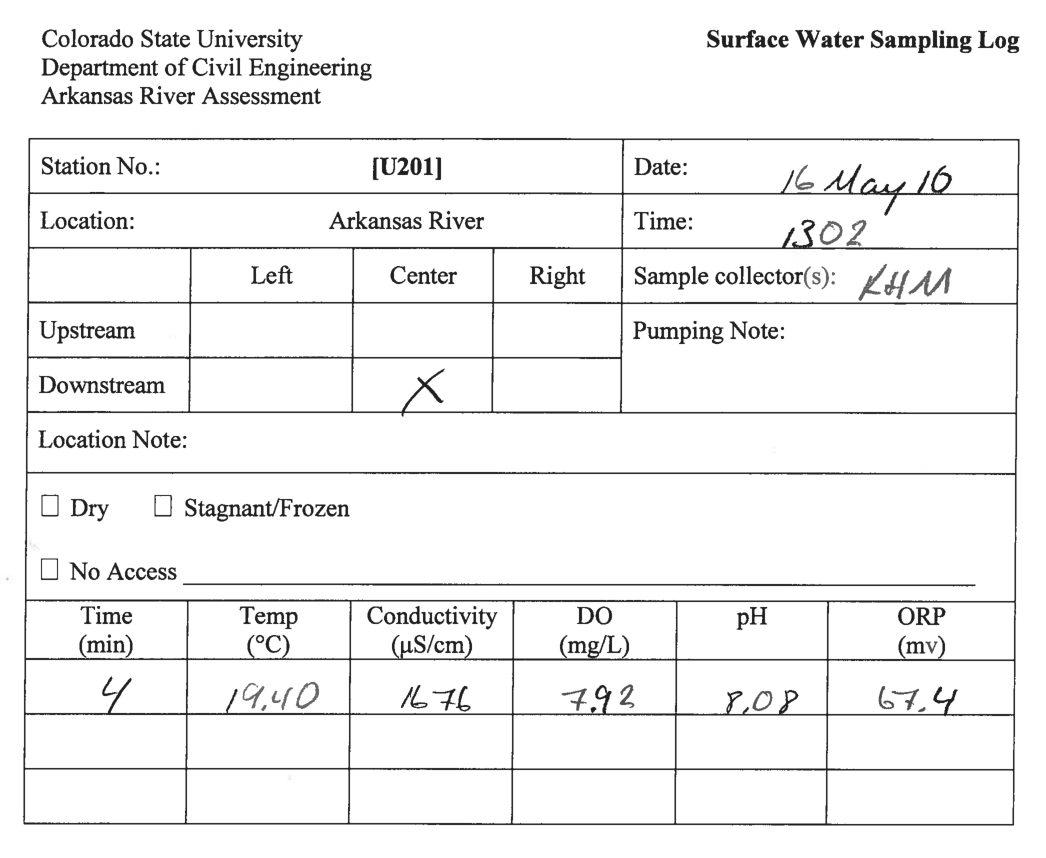
\includegraphics[width=6in]{Figures/SampleLogFilled}
	\caption[Example completed water quality sample form.]{Example completed water quality sample form.}
	\label{fig:samplogComplete}
\end{figure}

Specific ion lab results from Ward Laboratories and dissolved U lab results from TestAmerica were not used directly in the analysis reported in this tesis.  The Oscar E. Olson Biochemistry Laboratories (Olson Labs) at South Dakota State University (SDSU) performed dissolved Se analysis using Official Methods of Analysis of AOAC International, 17th Edition, test number 996.16, Selenium in Feeds and Premixes.  This test, a fluorometric test initially designed for testing animal feeds, provides repeatable analysis for dissolved Se near criteria levels.  Double tests were completed on each sample and the average was reported.  The minimum reportable value was \SI{0.4}{\micro\gram\per\liter}.  

Late in 2011, the Olson Labs was closed by SDSU for funding reasons.  Staff at Olson Labs assisted CSU staff in finding a new lab capable of continuing analyses using the same methods and to the same level of quality.  South Dakota Agricultural Laboratories (SDAL) was chosen.  Most of the staff and equipment from Olson Labs were employed at the new SDAL providing CSU staff with ample reason to move all dissolved Se analyses to the new lab.  Both Olson Labs and SDAL were certified by the USEPA for drinking water and subscribed to the proficiency testing and check sample programs for the USEPA for wastewaters \todo{ref.  How?}.

The same procedures and techniques for sample gathering and analysis were used during the entire sampling periods.  Newer or different techniques or procedures were considered, but was determined to have the possibility to compromise the consistency of the gathered data.  Results from all lab analyses were recorded in a master database at CSU for later data extraction and analysis.  The data includes results from over 4,500 sample sets.  Approximately 95 and 1,035 of these sample sets were taken from surface water sites in the USR and DSR, respectively.  Each sample set included in-situ measurements, a dissolved Se sample, a general specific ion panel, and a possible dissolved U sample.  In-situ EC and temperature measurements taken at stream gauge sites with permanent water quality instrumentation were compared with the measured values reported at those sites.  These sites record and report EC and water temperature measurements every 15-minutes.  Minor deviations were expected due to instrument drift and calibration error, yet EC and temperature differences were found to be less than 1\% for all in-situ measurements.

The water and mass balance models included in this study are among the many lines of research that have used this data.  Because of the multiple uses of large data sets, great care has been taken to ensure that data entry errors are rare.  Data were copied into the database and randomly checked for transcription errors.  Original lab reports were retained on file.

\clearpage{}
\section{River Cross-Section Geometry Survey}
The Arkansas River was surveyed at twenty-one and thirteen locations in the USR and DSR, respectively.  At these locations, cross-sections were surveyed and the data analyzed to determine the spatial distribution of the river geometry.  The cross-sections are not equally spaced along the river segments.  Cross-sections were surveyed at the extreme upstream and downstream end of each river segment.  Intermediate cross-sections were located where both the landowner permitted access and the river was reasonably accessible.  Additionally, the intermediate cross-sections were located where different cross-section profiles existed.  This was done to capture a broadest possible range of cross-section profiles, thereby allowing for a more realistic characterization of the river geometry.  Figures \ref{map:USRSurveyLocations} and \ref{map:DSRSurveyLocations} show the locations of the surveyed cross-sections in the USR and DSR, respectively.  Tables \ref{tab:USRSurveyLoc} and \ref{tab:DSRSurveyLoc} describe the location of the survey point with respect to the river reach and segment.  Survey locations within a river segment are with respect to the segment stream gauge location.

% Map - USR survey locations
\afterpage{%
	\clearpage%
	\begin{landscape}
	\begin{figure}[htbp]
		\centering
		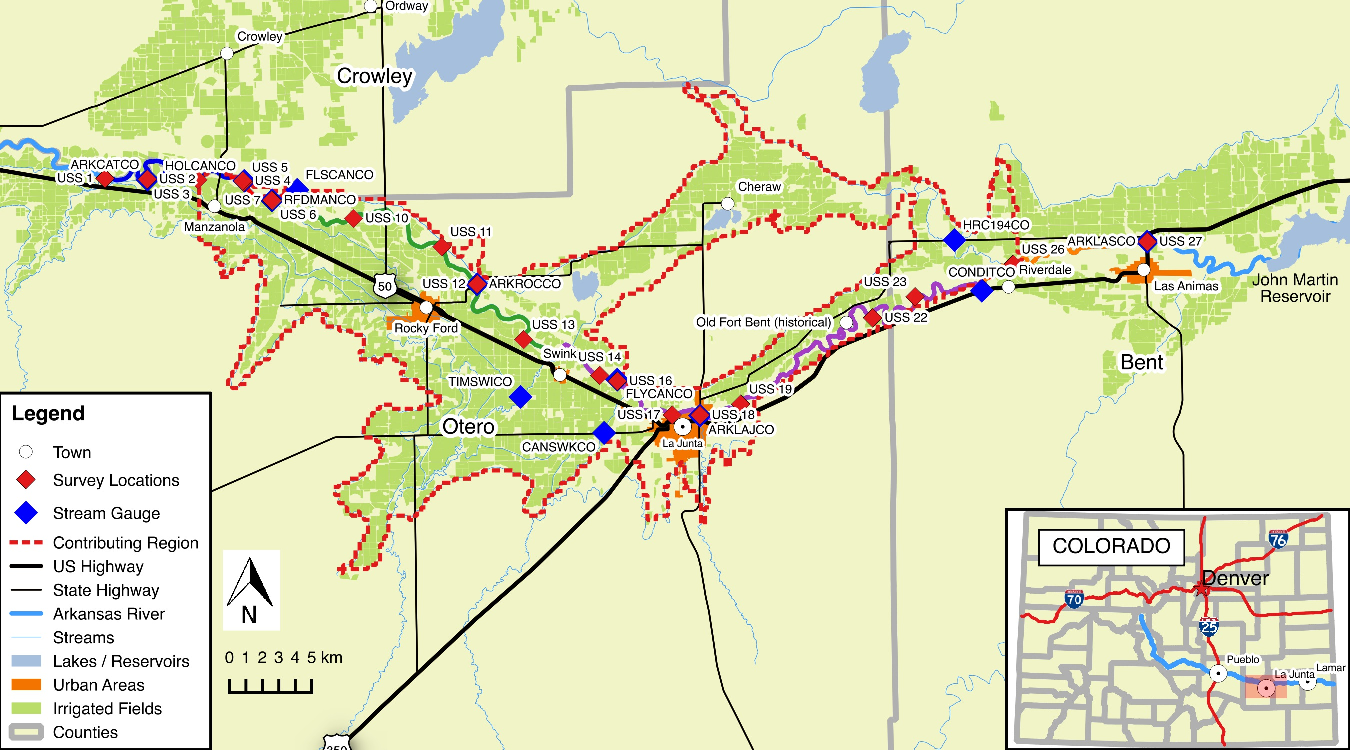
\includegraphics[scale=1]{Figures/Map/USRSurvey}
		\caption[USR River Cross-section Survey Locations.]{USR River Cross-section Survey Locations.  Cross-sections are taken above and/or below the diversion structure and near gauge locations.}
		\label{map:USRSurveyLocations}
	\end{figure}
	\end{landscape}
}

% Map - DSR survey locations
\afterpage{%
	\clearpage%
	\begin{landscape}
	\begin{figure}[htbp]
		\centering
		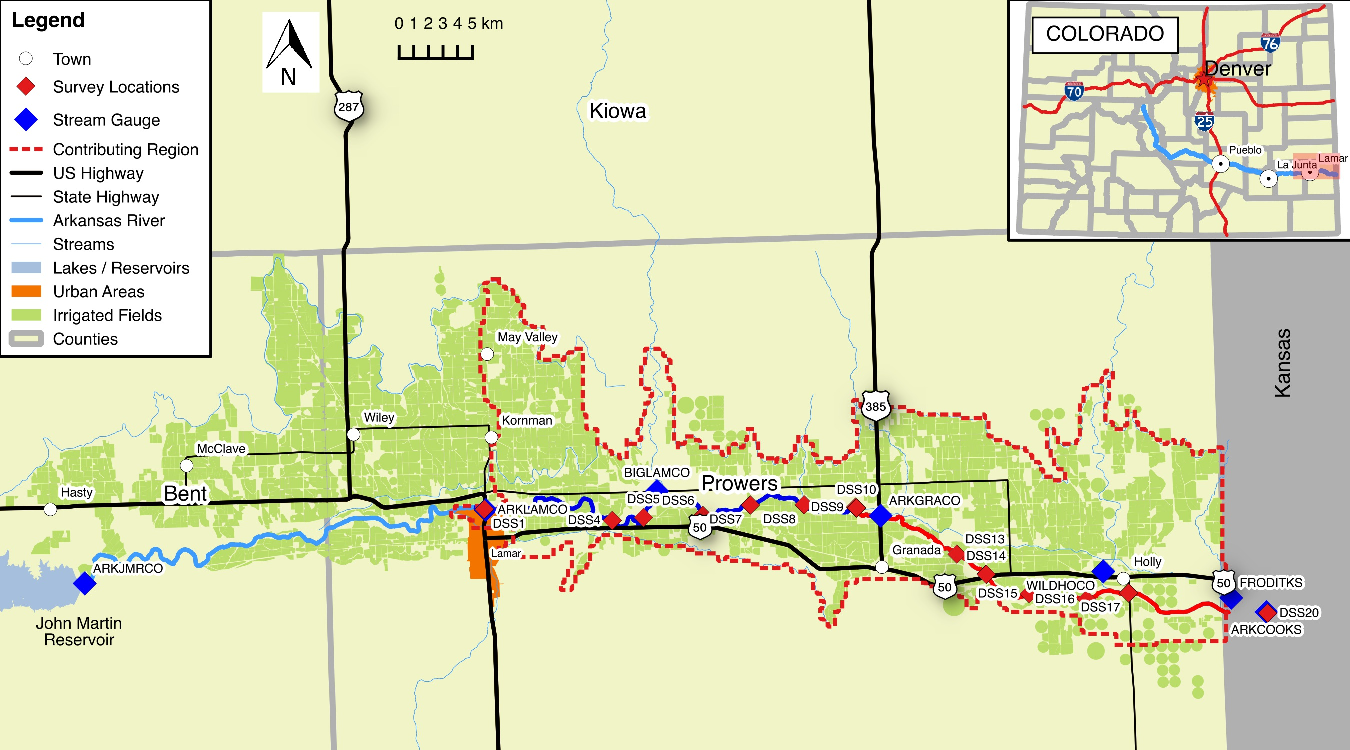
\includegraphics[scale=1]{Figures/Map/DSRSurvey}
		\caption[DSR River Cross-section Survey Locations.]{DSR River Cross-section Survey Locations.  Cross-sections are taken above and/or below the diversion structure and near gauge locations.}
		\label{map:DSRSurveyLocations}
	\end{figure}
	\end{landscape}
}

% Table - USR survey locations
\begin{table}[htbp]
	\centering
	\caption[Upstream Study Region (USR) Survey Point Information.]{Upstream Study Region (USR) Survey Point Information.  A value of zero (0) indicates the location of the segment stream gauge.  Negative distances indicate the point is upstream of the reference stream gauge location. Segment B does not contain a stream gauge on the river main stem.}
	\label{tab:USRSurveyLoc}
	\begin{tabular}{cccccc}
		\toprule
		River                       & Survey &  \multicolumn{2}{c}{Dist from}   &   \multicolumn{2}{c}{Dist from}   \\
		Segment                      & Point  & \multicolumn{2}{c}{USR Upstream} & \multicolumn{2}{c}{River Segment} \\
		Name                        &        &   \multicolumn{2}{c}{Boundary}   & \multicolumn{2}{c}{Stream Gauge}  \\
		\cmidrule(r{.5em}l){3-4} \cmidrule(r{.5em}l){5-6} &        &  mi  &            km             &  mi  &             km             \\ \toprule
		\multirow{4}{*}{A}                 &  USS1  &  0   &             0             & -2.7 &            -4.3            \\
		&  USS2  & 2.7  &            4.3            &  0   &             0              \\
		&  USS3  & 5.8  &            9.3            & 3.1  &             5              \\
		&  USS4  & 7.8  &           12.6            & 5.1  &            8.2             \\ \midrule
		\multirow{3}{*}{B}                 &  USS6  & 9.2  &           14.8            &      &  \\
		&  USS7  & 9.3  &           14.9            &      &  \\
		&  USS8  & 10.2 &           16.4            &      &  \\ \midrule
		\multirow{5}{*}{C}                 & USS10  & 13.4 &           21.6            & -6.8 &           -10.9            \\
		& USS11  & 18.1 &           29.1            & -2.1 &            -3.4            \\
		& USS12  & 20.2 &           32.5            &  0   &             0              \\
		& USS13  & 24.4 &           39.3            & 4.2  &            6.8             \\
		& USS14  & 29.3 &           47.2            & 9.1  &            14.6            \\ \midrule
		\multirow{7}{*}{D}                 & USS16  &  30  &           48.3            & -3.8 &            -6.1            \\
		& USS17  & 32.6 &           52.5            & -1.2 &            -1.9            \\
		& USS18  & 33.8 &           54.4            &  0   &             0              \\
		& USS19  & 35.9 &           57.8            & 2.1  &            3.4             \\
		& USS21  &  44  &           70.8            & 10.2 &            16.4            \\
		& USS22  & 46.4 &           74.7            & 12.6 &            20.3            \\
		& USS23  & 50.3 &            81             & 16.5 &            26.6            \\ \midrule
		\multirow{2}{*}{E}                 & USS26  & 55.7 &           89.6            &  -6  &            -9.7            \\
		& USS27  & 61.7 &           99.3            &  0   &             0              \\ \bottomrule
	\end{tabular}
\end{table}

% Table - DSR survey locations
\begin{table}[htbp]
	\centering
	\caption[Downstream Study Region (DSR) River Cross-Section Survey Location Information.]{Downstream Study Region (DSR) River Cross-Section Survey Location Information.  A value of zero (0) indicates the location of the segment stream gauge.  Negative distances indicate the point is upstream of the reference stream gauge location.}
	\label{tab:DSRSurveyLoc}
	\begin{tabular}{cccccc}
		\toprule
		River                        & Survey &  \multicolumn{2}{c}{Dist from}   &   \multicolumn{2}{c}{Dist from}   \\
		Segment                       & Point  & \multicolumn{2}{c}{USR Upstream} & \multicolumn{2}{c}{River Segment} \\
		Name                         &        &   \multicolumn{2}{c}{Boundary}   & \multicolumn{2}{c}{Stream Gauge}  \\
		\cmidrule(r{0.5em}l){3-4} \cmidrule(r{0.5em}l){5-6} &        &  mi  &            km             &  mi  &             km             \\ \toprule
		\multirow{7}{*}{F}                  &  DSS1  &  0   &             0             &  0   &             0              \\
		&  DSS4  & 7.9  &           12.7            & 7.9  &            12.7            \\
		&  DSS5  & 10.3 &           16.6            & 10.3 &            16.6            \\
		&  DSS6  & 14.9 &            24             & 14.9 &             24             \\
		&  DSS7  & 17.6 &           28.3            & 17.6 &            28.3            \\
		&  DSS8  & 20.5 &            33             & 20.5 &             33             \\
		&  DSS9  & 23.4 &           37.7            & 23.4 &            37.7            \\ \midrule
		\multirow{6}{*}{G}                  & DSS10  & 23.5 &           37.8            & -1.4 &            -2.3            \\
		& DSS13  & 29.3 &           47.2            & 4.4  &            7.1             \\
		& DSS14  & 31.2 &           50.2            & 6.3  &            10.1            \\
		& DSS15  & 33.9 &           54.6            &  9   &            14.5            \\
		& DSS16  &  37  &           59.5            & 12.1 &            19.5            \\
		& DSS17  & 38.9 &           62.6            &  14  &            22.5            \\ \midrule
		& DSS20  & 46.2 &           74.4            &      &  \\ \bottomrule
	\end{tabular}
\end{table}

Industry standard survey techniques were used whenever possible.  It was not possible to properly locate the instrument location in either the horizontal and vertical plane with respect to a local datum due to the remote location and the lack of available time.  All data was collected with a total station (Figure \ref{pic:surveySub1})and hand recorded into survey log books.  Two back-sights were used at every surveyed cross-section.  Both back-sights and the instrument location were located by using a hand held global positioning satellite (GPS) receiver (Figure \ref{pic:surveySub2}).  The receiver was capable of determining the horizontal location to within \SI{\pm 1}{\meter} and the vertical location to within \SI{\pm 2}{\meter}.  Licensed surveyors were not hired, retained, or consulted for this study.

% Picture - total station and GPS
\begin{figure}[htbp]
	\subcaptionbox{Pentax PCS-315 Total Station.\label{pic:surveySub1}}{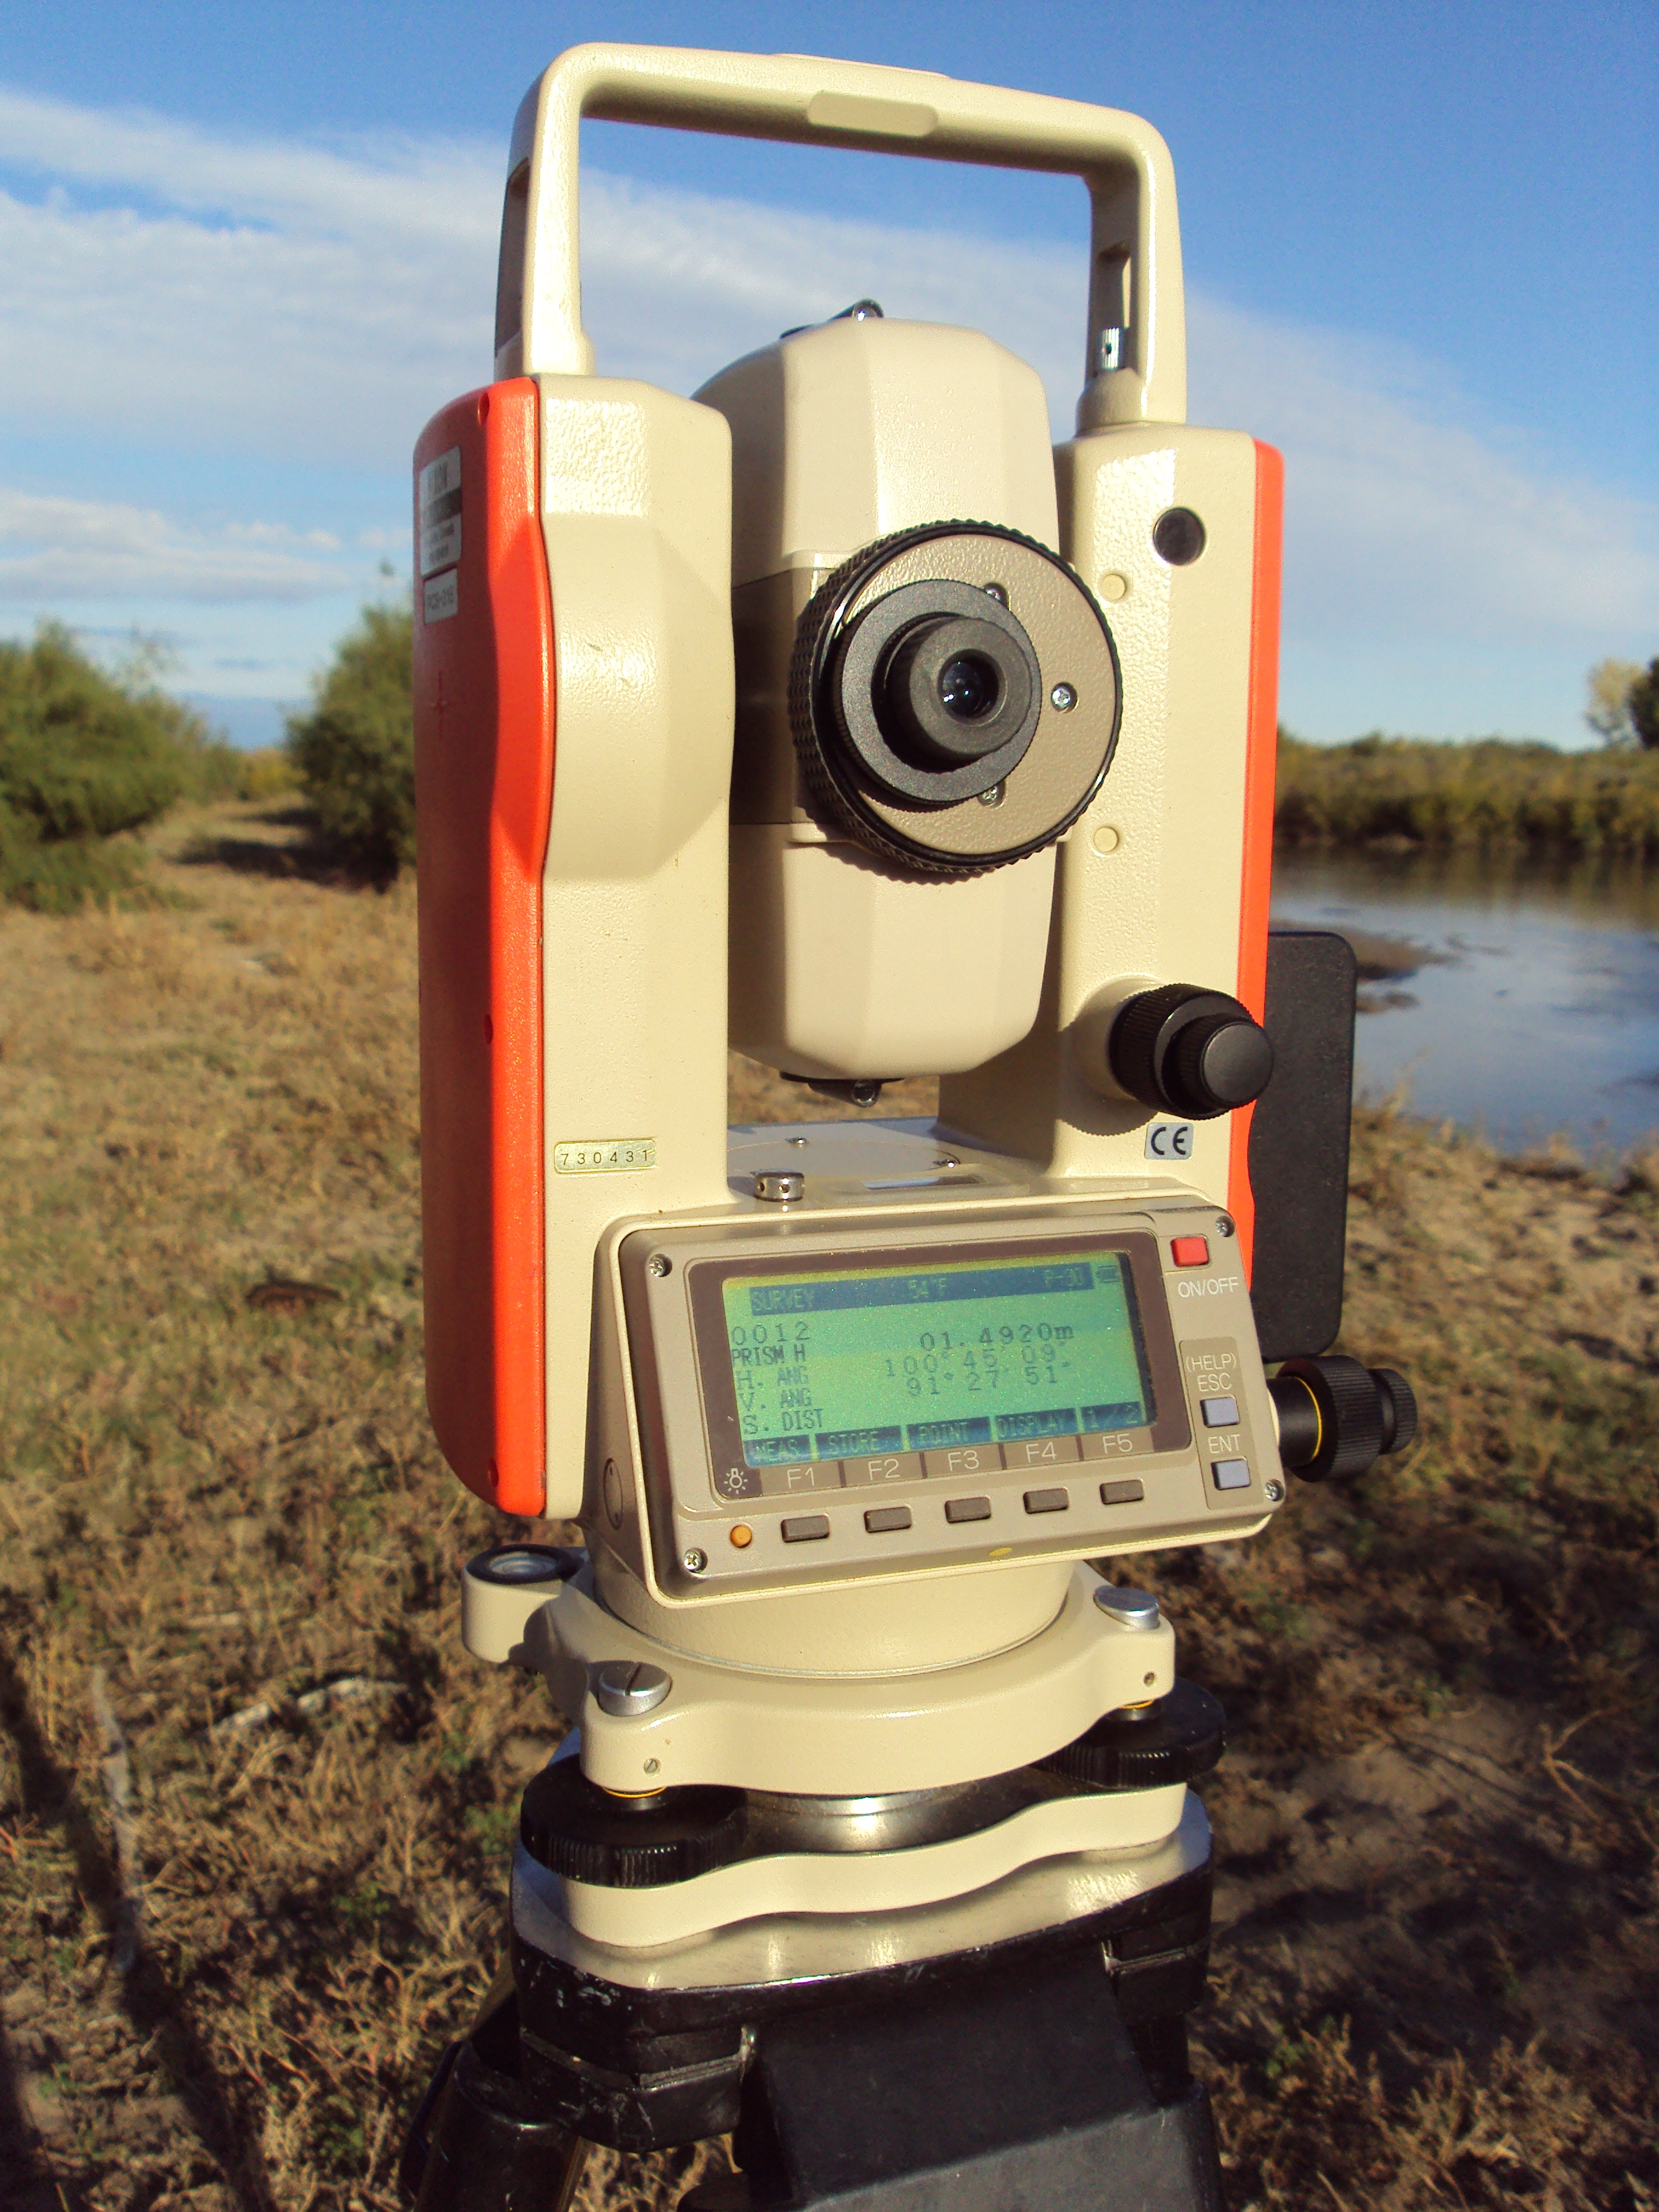
\includegraphics[width=2.5in]{Figures/Photo/TotalStation}}\hspace{4em}%
	\subcaptionbox{TopCon GMS-2 Sub-meter handheld GPS.\label{pic:surveySub2}}{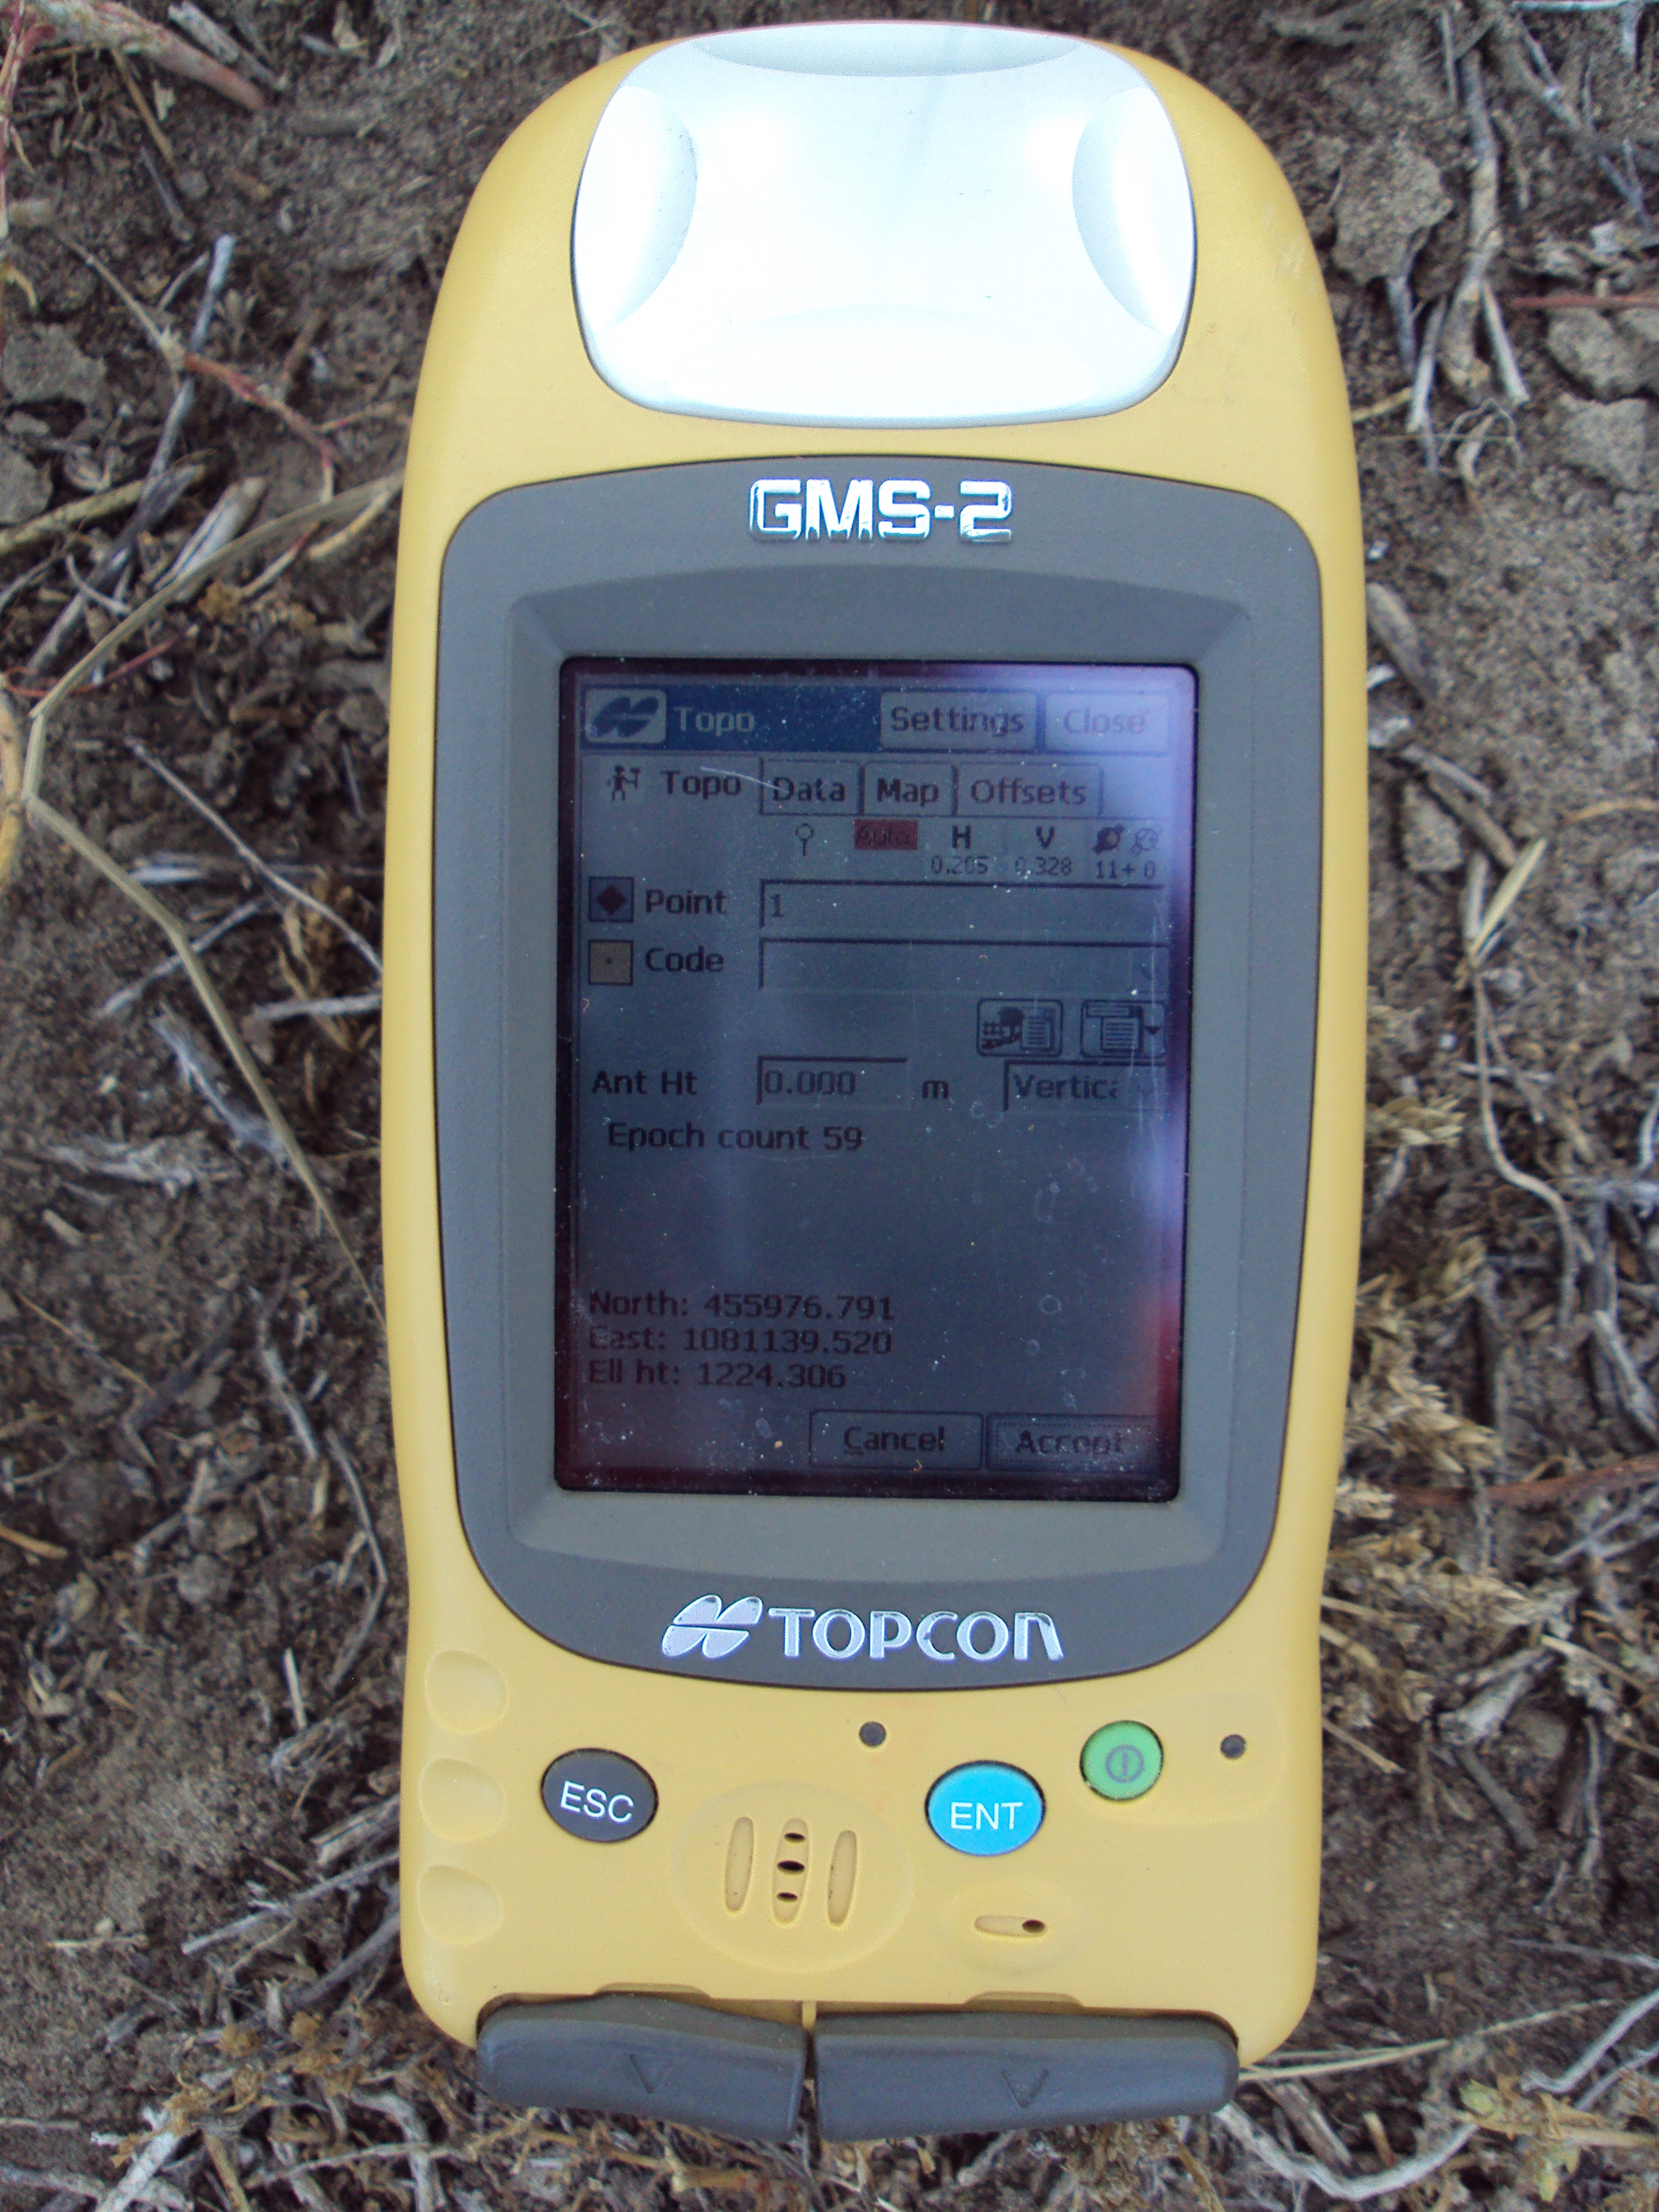
\includegraphics[width=2.5in]{Figures/Photo/SubMeterGPS2}}
	\caption[Survey Equipment.]{Survey Equipment.}
	\label{pic:surveyEquip}
\end{figure}

Higher location and orientation accuracy could have been obtained by using survey grade GPS equipment or by referencing the instrument survey to an established benchmark.  For almost all surveyed cross-sections, benchmarks were not located within a reasonable distance.  Attempting to tie into these benchmarks would results in an order of magnitue or more increase in the time required to complete the survey.  There were also doubts as to whether the horizontal and vertical accuracy could be maintained due to the distance between the nearest benchmarks and the survey sites and the surveyor's skill.  Survey grade GPS equipment could have been used, but would have required either a larger team or a significantly increased risk of equipment tampering or theft.  The available survey grade GPS base station also had a limited range compared to the range required to access many of the locations.  Since the goal of the survey was to determine the relationship between the depth and width of the river, it was determined that locating and orienting the survey data correctly was a secondary goal. For these reasons, it was determined that the level of location and orientation accuracy obtained by using the hand held GPS receiver would be sufficient.

The data was collected in the form of horizontal angle, vertical angle, sight distance, rod height, and instrument height.  The survey data was downloaded from the total station and entered into a spreadsheet for conversion to horizontal and vertical location relative to the instrument.  Values in the spreadsheet were checked against the survey log book.  Points collected but not used to calculate the cross-section, such as the back-sight points, were marked so that they were not used in the cross-section analysis.  These excluded points were used for other survey related calculations.  The rod height for each measurement and the instrument height for the survey was transferred from the log book to the spreadsheet.  

Coordinate geometry (COGO) techniques were used to convert from angle, sight distance, rod height, and instrument height measurements to horizontal and vertical distance measurements relative to the instrument as shown in figure \ref{fig:SurveyMeasurements}.  Vertical angles were measured using decimal degrees such that zero degrees (\SI{0}{\degree}) was located above the instrument and \SI{90}{\degree} was horizontal.  Horizontal angles were measured using decimal degrees such that \SI{0}{\degree} was located when the instrument was facing the first back-sight and positive angles were measured clockwise when viewed from above.  The sight distance was measured using the instruments integrated laser distance measuring tool from the optics of the instrument to the rod prism with sub-millimeter accuracy.  Horizontal and vertical distances to the ground location of the survey point from the ground location of the instrument were calculated as shown in equations \ref{eq:horizontal} and \ref{eq:vertical}, respectively.  The horizontal location was calculated as northing and easting with the line between the instrument and the first back-sight as the reference.  Northing and easting distances were calculated with respect to the horizontal line between the instrument and the first backsight.  Corrections were made to orient the points to the coordinate system, but this step was not necessary to provide the necessary results. %as shown in equations \ref{eq:northing} and \ref{eq:easting}, respectively.

% Figure - Survey measurements.  Includes equation.
\begin{figure}[htbp]
	\centering
	\includegraphics[scale=1]{Figures/LineDiagram/SurveyMeasurements}

\begin{align}
	d_h=&\:d_s \cdot sin(\theta_v) \label{eq:horizontal} \\
	\nonumber \\
	d_v=&\:h_i-h_r+d_s \cdot cos(\theta_v) \label{eq:vertical}
\end{align}
%	d_N=&d_h \cdot cos(\theta_h) \label{eq:northing} \\  %% took out the horizontal measurements.  Not particularly relevant.
%	d_E=&d_h \cdot sin(\theta_h) \label{eq:easting}
\begin{tabular}{r l}
	        $d_h$ = & Horizontal distance from the instrument to the surveyed point.                    \\
	        $d_v$ = & Vertical distance from the instrument to the surveyed point.                      \\
	      %	$d_N$ = & Horizontal distance from the instrument to the surveyed point as projected on the \\
	              % & East-West line passing through the instrument (northing).                         \\
	              % &  \\
	      %	$d_E$ = & Horizontal distance from the instrument to the surveyed point as projected on the \\
	              % & North-South line passing through the instrument (easting).                        \\
	              % &  \\
	        $d_s$ = & Sight distance from the instrument optics to the rod prism.                       \\
	   $\theta_v$ = & Vertical angle from the sight optics to the rod prism                             \\
	%	$\theta_h $ = & Horizontal angle from the sight optics to the rod prism                           \\
	              % &
\end{tabular}
	\caption[Survey Measurement Definitions.]{Survey Measurement Definitions.}
	\label{fig:SurveyMeasurements}
\end{figure}

GPS location data for the instrument and back-sights was collected in the form of northing, easting, and elevation.  Colorado State Plane-South, North American Datum 1983 (NAD83), U.S. feet was used as the horizontal datum and North American Vertical Datum 1988 (NAVD88) was used as the vertical datum.  All survey units are U.S. Feet.  Survey errors, also known as closing errors, were corrected for all points.  Most survey locations were on soft soils.  It was assumed that survey error would primarily consist of instrument location drift.  Measurements were taken to both back-sights at the beginning an end of the site survey.  The northing, easting, and elevation difference between the measurements taken at the beginning and end of the site survey were spread equally and successively among all points.  Since two back-sights were used, the total closing error was taken as the average of the closing errors for the two back-sights.  

Correction of closing errors was required to obtain accurate stream depth and river top width values.  Location and orientation error correction was not required and was only performed as a manner of good survey practice.  Survey data points were translated from their position relative to the instrument to their position relative to the State Plane coordinate system by adding the northing, easting, and elevation values collected by the GPS receiver at the instrument site.  Orientation error corrections to make instrument North coincide with true North were made by adding a positive horizontal correction angle such that the corrected angle to the first back-sight, which was the zero back-sight, matched the angle between the two corresponding GPS northing and easting coordinate sets.  Final survey locations should always have the most correct location and elevation relative to a given datum.  Both the back-sights and instrument location were marked with steel reinforcement bar (re-bar) and plastic caps (Figure \ref{pic:plasticCap}), it may be possible for future surveys to be conducted at the same locations with the same back-sights.

% Picture - control point/plastic cap
\begin{figure}[htbp]
\centering
	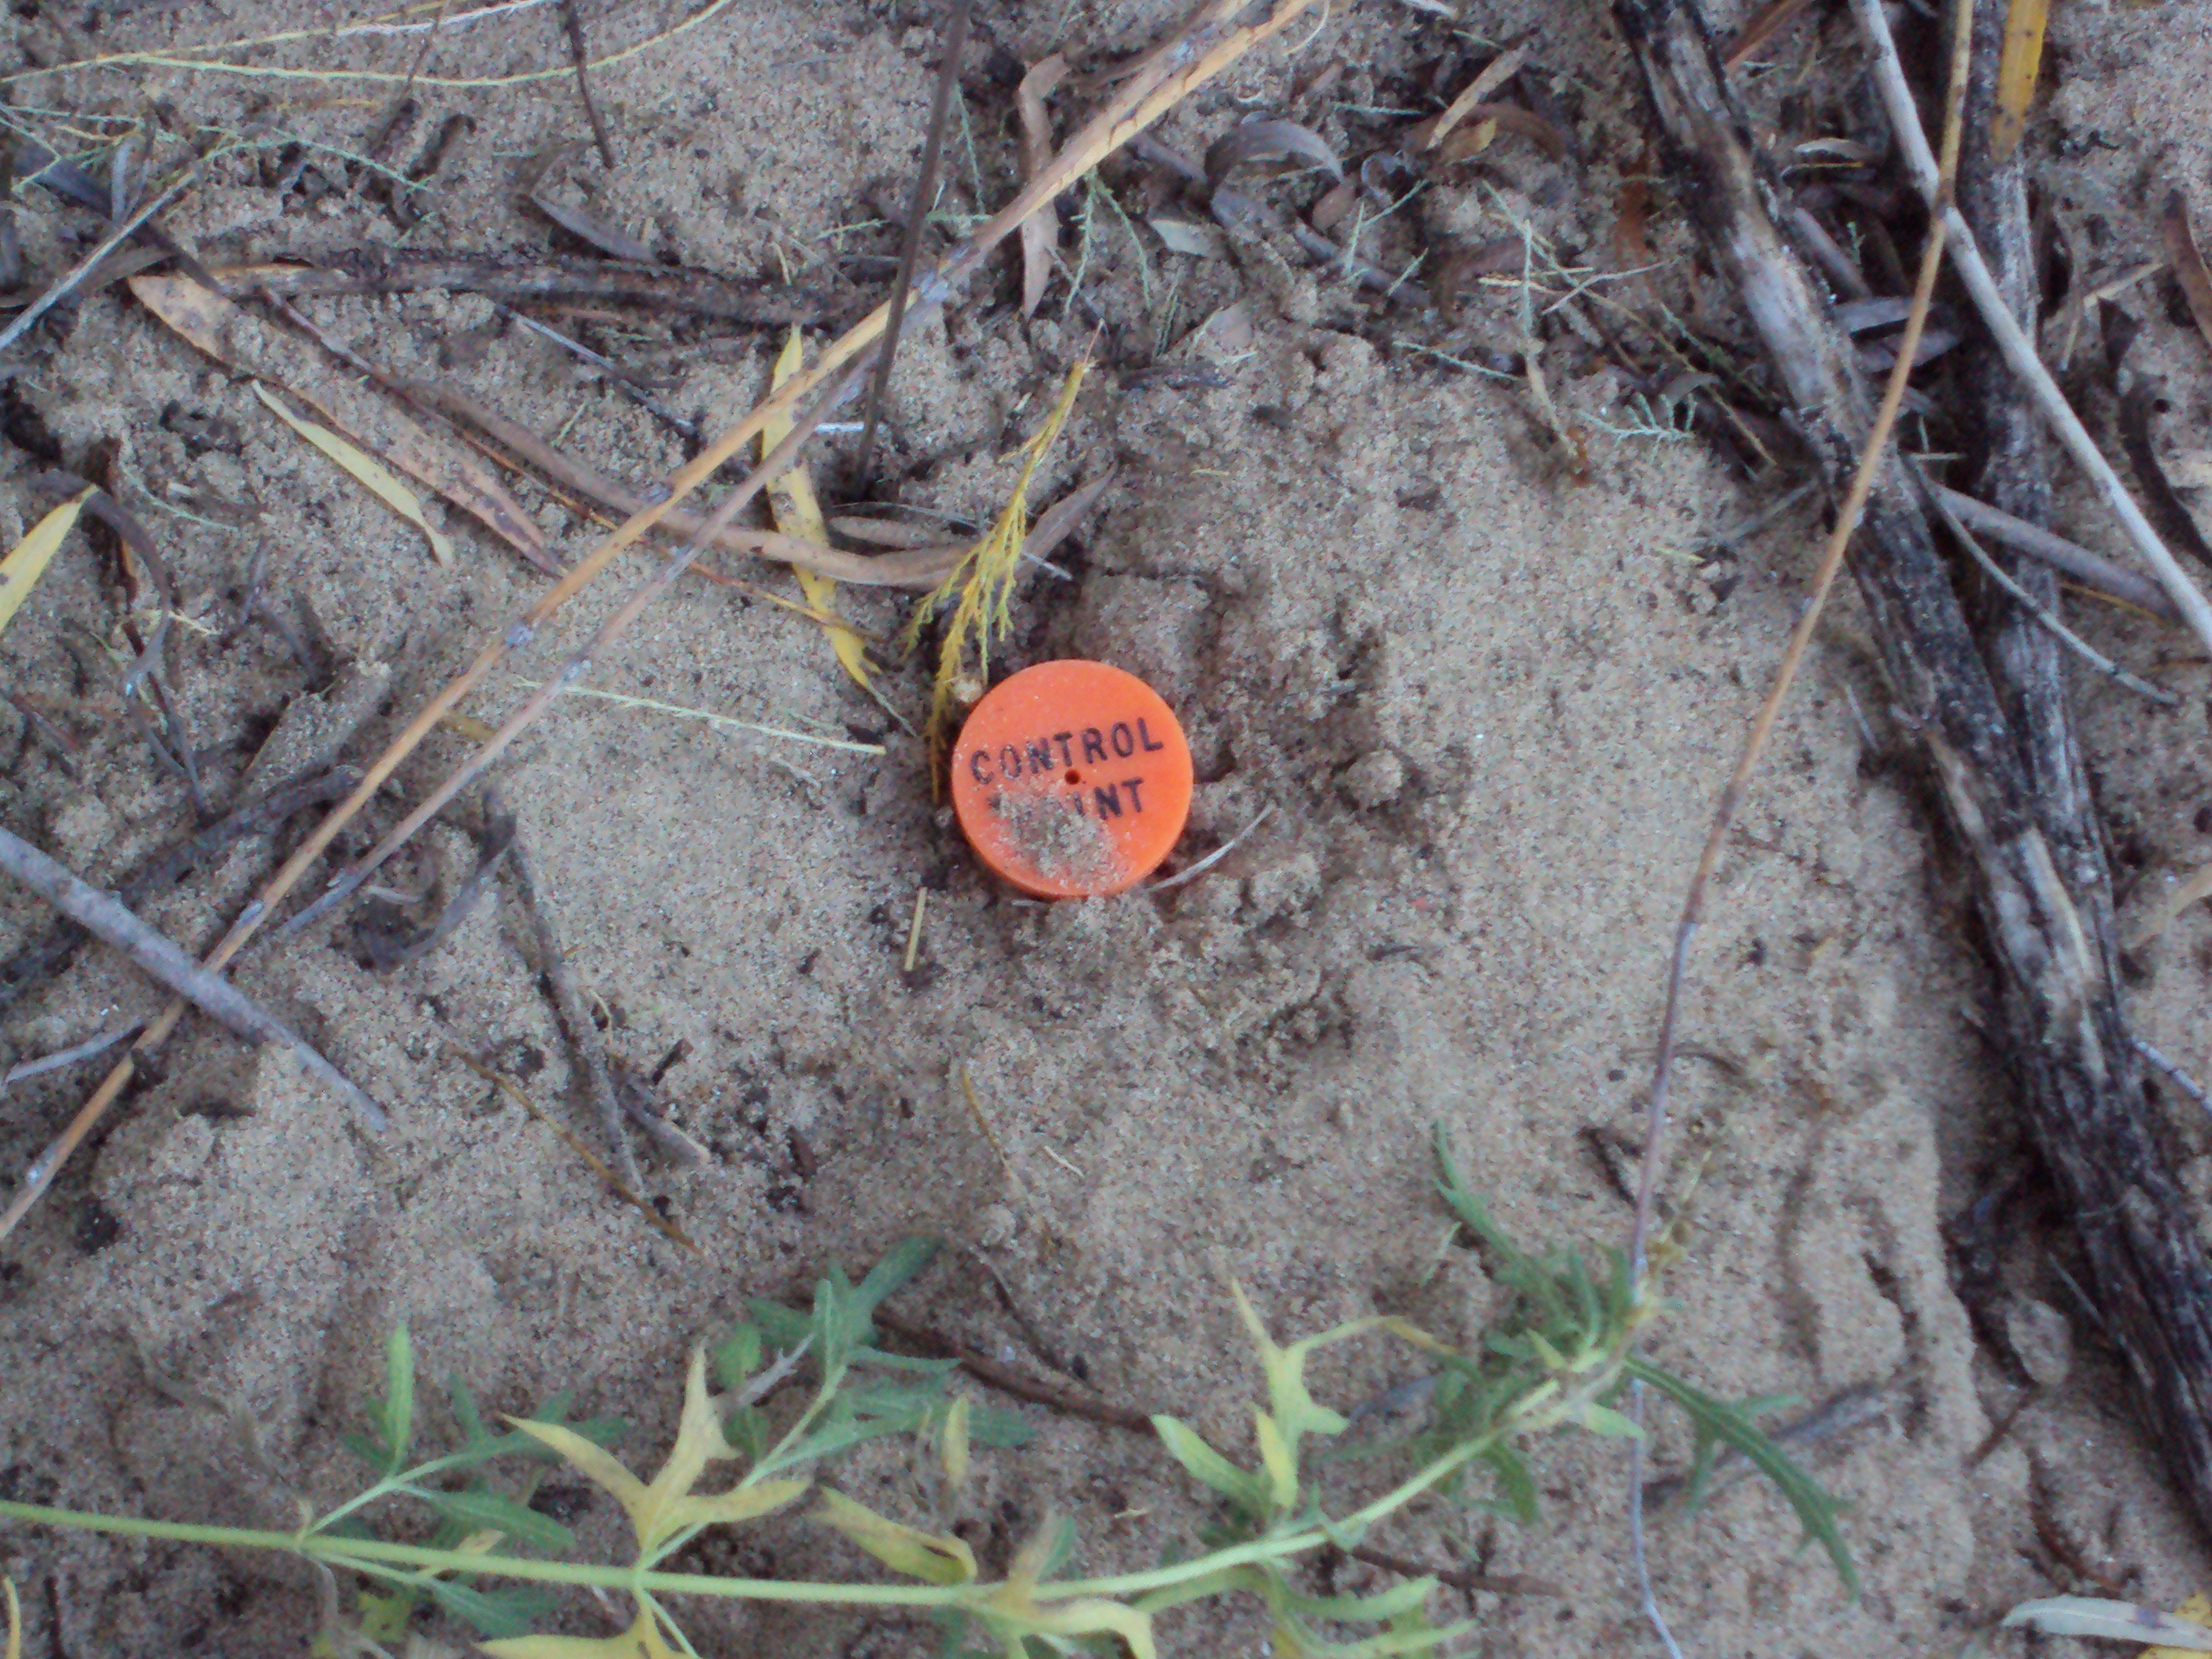
\includegraphics[width=3in]{Figures/Photo/ControlPoint}
	\caption[Typical plastic cap on rebar used to locate instrument location and back-sights.]{Typical plastic cap on rebar used to locate instrument location and back-sights.}
	\label{pic:plasticCap}
\end{figure}

A least squares fit linear regression equation was fit to the relative location of all points along the surveyed cross-section (Figure \ref{fig:SurveyPlanView}).  It was reasoned that a straight line through the data points would allow for a better approximation of the river's cross-section than connecting the points.  The straight line would represent a true cross-section, whereas connecting the points would exaggerate the distance across the cross-section.  The relative locations of the points as projected onto the best-fit line were entered into computer aided design and drafting (CADD) software (Figure \ref{fig:SurveySection}).  Horizontal lines, spaced 0.03 m (0.1 ft) apart from the bottom of the channel to 1.5 m (5 ft) from the bottom, were drawn from edge of bank to edge of bank.  The vertical location of these lines was taken as the flow depth and the length of the line was taken as the river top width.

% Figure - Translate survey points to horizontal best fit line.
\begin{figure}[htbp]
\centering
	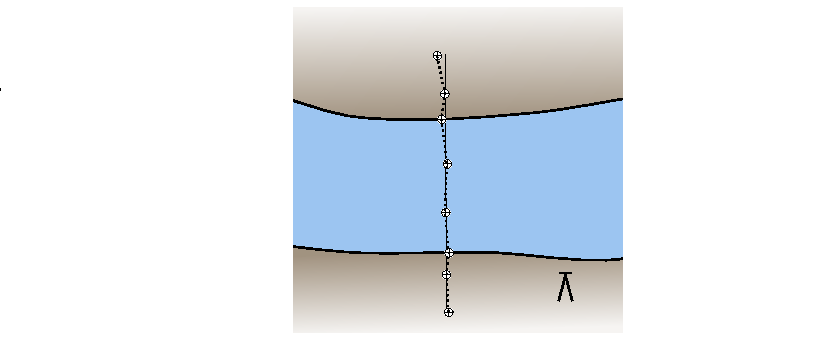
\includegraphics[width=6in]{Figures/LineDiagram/SurveyPlanView}
	\caption[Depiction of the conversion of River Survey Locations to Linear Cross-Section.]{Depiction of the conversion of River Survey Locations to Linear Cross-Section.  The crossed circles are the surveyed points.  The instrument (total station) is in the lower right-hand corner.  The dotted line depicts the cross section if no correction were made to linearize the survey cross section locations.  The solid line is the cross-section line created from the best-fit line through the surveyed points.  Surveyed points were translated perpendicular to the cross-section line to lie on the cross-section line across the river.}
	\label{fig:SurveyPlanView}
\end{figure}

% Figure - CADD drawing of cross section with no vertical exageration
\begin{figure}[htbp]
\centering
	\includegraphics[width=6in]{Figures/LineDiagram/USS1Trim}
	\caption[River Cross-Section as Draw in CADD Software.]{River Cross-Section as Draw in CADD Software.  The black line is the channel cross-section with the left side representing the north bank of the Arkansas River (water flow is into the page).  The blue horizontal line is the lowest point in the surveyed channel.  All elevations were shifted such that the bottom point had a stream depth of zero.  This particular cross section is at cross-section USS1.  The horizontal and vertical scales are identical.}
	\label{fig:SurveySection}
\end{figure}

%Each surveyed point had two location value sets.  The first set being relative to the instrument without location and orientation corrections.  The second set being relative to the State Plane with corrections for location, orientation, and elevation.  The two data sets shall be referred to as relative location and State Plane location, respectively.  The State Plane location for each point is directly derived from the relative location.  All survey error corrections were applied to the relative locations before converting the data to State Plane locations.
%
%Location errors due to GPS accuracy issues were corrected by comparing the State Plane location of the two back-sights to the GPS surveyed location at those sights.  The average difference in northing, easting, and elevation between the GPS back-sight coordinates and the instrument surveyed coordinates was used to shift the State Plane location of the instrument.  The State Plane location of all points was re-calculated after performing this correction.

\clearpage{}
\section{Data Compiled from Other Sources}
\label{sec:data collected by other sources}
The data collected in the field constituted a small portion of the total data required to perform water and mass balance calculations.  Additional data were obtained from three sources: the USGS, the CDWR, and the Colorado Climate Center (CCC).

The USGS operates and maintains the largest network of stream gauges in the United States.  USGS gauges in the LARV in Colorado are operated and maintained by the USGS Colorado Water Science Center.  Their main office is Lakewood, Colorado, with one of their satellite offices in Pueblo, Colorado.  Of the gauges listed in Tables \ref{tab:USRGauges} and \ref{tab:DSRGauges} and shown in Figures \ref{map:USRGaugeLocations} and \ref{map:DSRGaugeLocations}, five are operated by the USGS.  There is additional sensing equipment owned and maintained by the USGS at some stream gauges owned and operated by the CDWR.  Water temperature, air temperature, precipitation, and EC are the additional parameters typically measured and recorded by this equipment.  EC is reported as specific conductance standardized to \SI{25}{\degreeCelsius} and is the standard for EC used throughout this thesis.  EC values are reported in units of micro-siemens per centimeter (\si{\micro\siemens\per\centi\meter}) and are converted to units of deci-siemens per meter (\si{\deci\siemens\per\meter}).

% Map - USR stream gauge locations
\afterpage{%
	\clearpage%
	\begin{landscape}
		\begin{figure}[htbp]
			\centering
			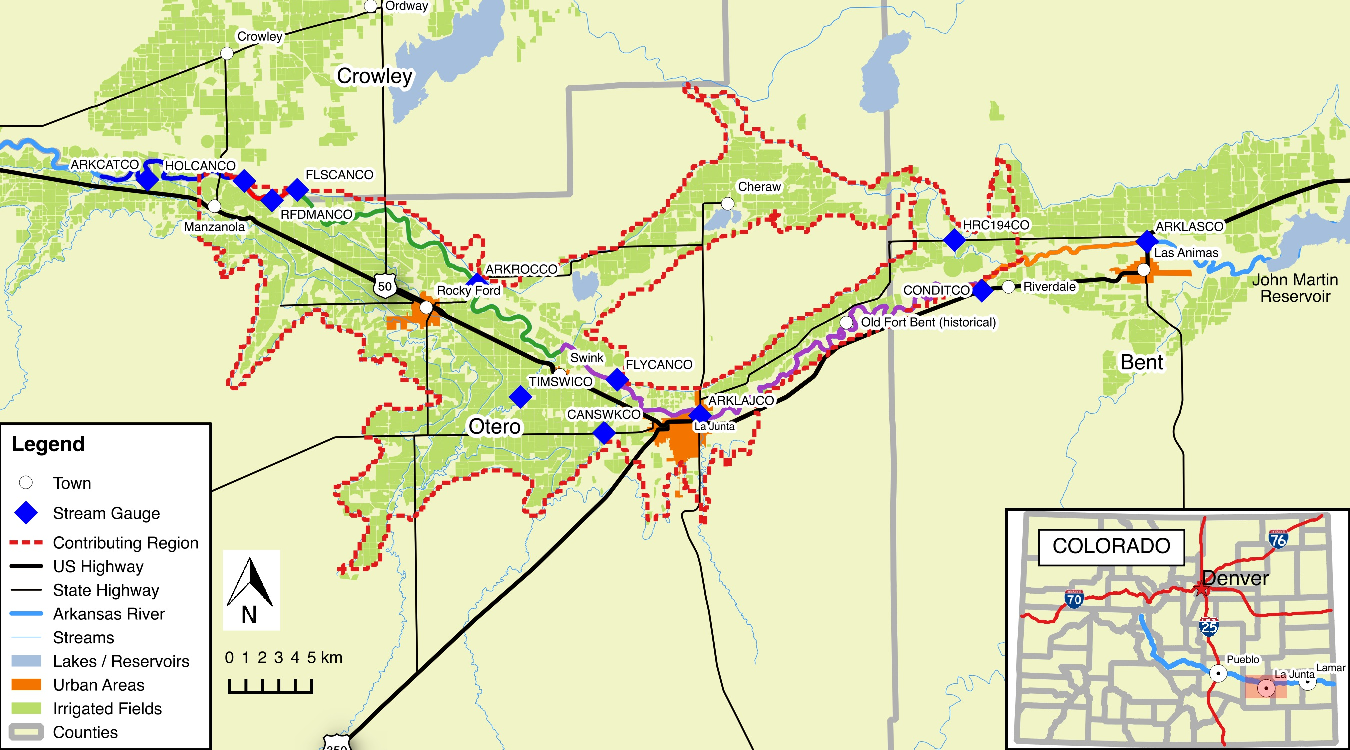
\includegraphics[scale=1]{Figures/Map/USRGauge}
			\caption[USR River and Tributary Stream Gauge Locations.]{USR River River and Tributary Stream Gauge Locations.}
			\label{map:USRGaugeLocations}
		\end{figure}
	\end{landscape}
}

% Map - DSR stream gauge locations
\afterpage{%
	\clearpage%
	\begin{landscape}
		\begin{figure}[htbp]
			\centering
			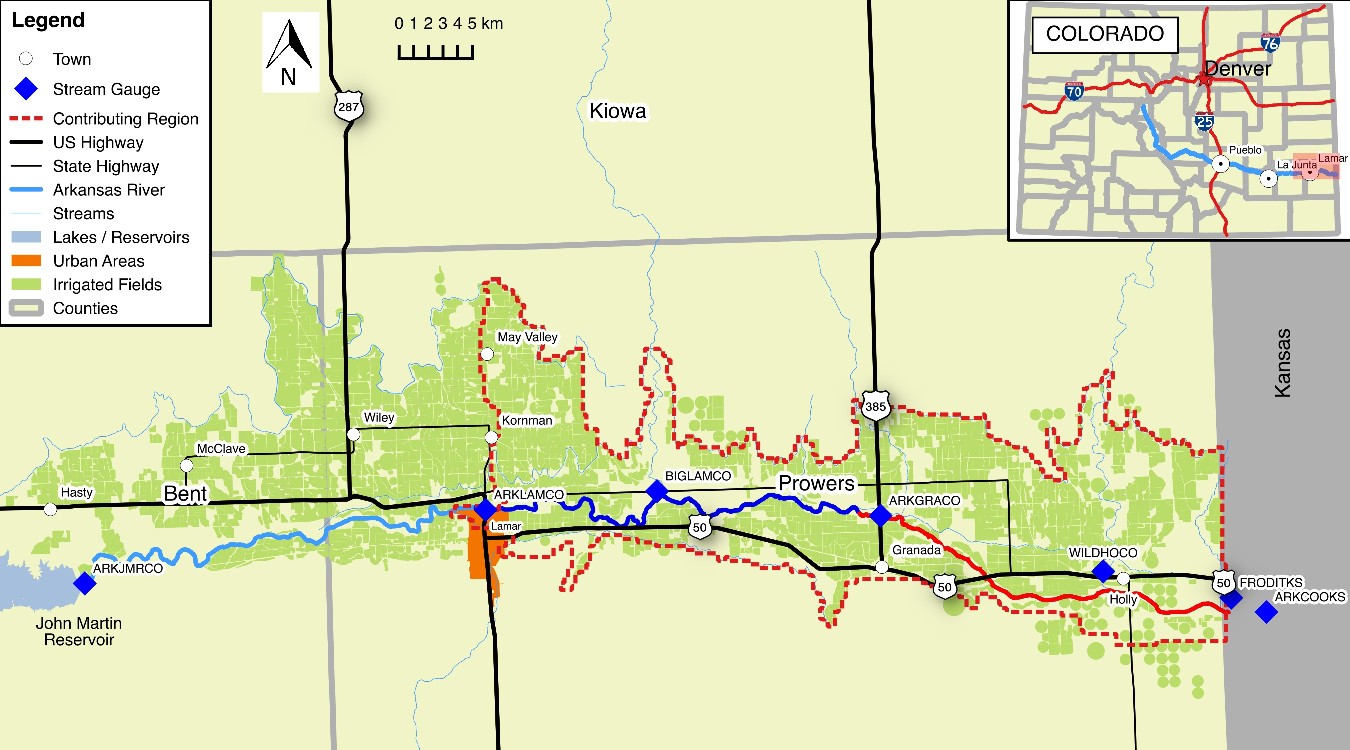
\includegraphics[scale=1]{Figures/Map/DSRGauge}
			\caption[DSR River and Tributary Stream Gauge Locations.]{DSR River River and Tributary Stream Gauge Locations.}
			\label{map:DSRGaugeLocations}
		\end{figure}
	\end{landscape}
}



% Table - USR stream gauge locations
\begin{table}[htbp]
\centering
  \caption[Upstream Study Region (USR) Stream Gauge Information.]{Upstream Study Region (USR) Stream Gauge Information.  Segment stream gauges record flow depth for surface area and river volume change calculations.  A value of zero (0) indicates the location of the segment stream gauge.  Negative distances indicate the point is upstream of the reference stream gauge location. Segment B does not contain a stream gauge on the river main stem.}
    \label{tab:USRGauges}
\begin{tabular}{ccccccc}
	\toprule
	                      River                       &     CDWR     &     USGS     &  \multicolumn{2}{c}{Dist. from}  &  \multicolumn{2}{c}{Dist. from}   \\
	                     Segment                      & Stream Gauge & Stream Gauge & \multicolumn{2}{c}{USR Upstream} & \multicolumn{2}{c}{River Segment} \\
	                      Name                        &     Name     &     Name     &   \multicolumn{2}{c}{Boundary}   & \multicolumn{2}{c}{Stream Gauge}  \\
	\cmidrule(r{.5em}l){4-5} \cmidrule(r{.5em}l){6-7} &              &              &  mi  &            km             &  mi  &             km             \\ \toprule
	               \multirow{2}{*}{A}                 &   ARKCATCO   &              & 2.7  &            4.3            &  0   &             0              \\
	                                                  &   HOLCANCO   &              & 7.8  &           12.6            & 5.1  &            8.2             \\ \midrule
	               \multirow{2}{*}{B}                 &   RFDMANCO   &              & 9.2  &           14.8            &      &  \\
	                                                  &   FLSCANCO   &              & 10.2 &           16.4            &      &  \\ \midrule
	               \multirow{4}{*}{C}                 &   RFDRETCO   &              & 11.7 &           18.8            & -8.5 &           -13.7            \\
	                                                  &   ARKROCCO   &              & 20.2 &           32.5            &  0   &             0              \\
	                                                  &   TIMSWICO   &   7121500    & 26.1 &            42             & 5.9  &            9.5             \\
	                                                  &   FLYCANCO   &              & 29.3 &           47.2            & 9.1  &            14.6            \\ \midrule
	               \multirow{3}{*}{D}                 &   CANSWKCO   &              & 30.3 &           18.8            & -3.5 &            -5.6            \\
	                                                  &   ARKLAJCO   &              & 33.8 &           54.4            &  0   &             0              \\
	                                                  &   CONDITCO   &              & 52.8 &            85             &  19  &            30.6            \\ \midrule
	               \multirow{2}{*}{E}                 &   HRC194CO   &              & 55.1 &           88.7            & -6.6 &           -10.6            \\
	                                                  &   ARKLASCO   &   7124000    & 61.7 &           99.3            &  0   &             0              \\ \bottomrule
\end{tabular}
\end{table}

% Table - DSR stream gauge locations
\begin{table}[htbp]
  \centering
  \caption[Downstream Study Region (DSR) Stream Gauge Information.]{Downstream Study Region (DSR) Stream Gauge Information.  River segment stream gauges record flow depth for surface area and river volume change calculations.  A value of zero (0) indicates the location of the segment stream gauge.  Negative distances indicate the point is upstream of the reference stream gauge location. Stream gauges ARKJMRCO, FRODITKS and ARKCOOKS although required for analysis, are not within the DSR.}
\label{tab:DSRGauge}
\begin{tabular}{ccccccc}
	\toprule
	                       River                        &     CDWR     &     USGS     &  \multicolumn{2}{c}{Dist. from}  &  \multicolumn{2}{c}{Dist. from}   \\
	                      Segment                       & Stream Gauge & Stream Gauge & \multicolumn{2}{c}{DSR Upstream} & \multicolumn{2}{c}{River Segment} \\
	                       Name                         &     Name     &     Name     &   \multicolumn{2}{c}{Boundary}   & \multicolumn{2}{c}{Stream Gauge}  \\
	\cmidrule(r{0.5em}l){4-5} \cmidrule(r{0.5em}l){6-7} &              &              &  mi  &            km             &  mi  &             km             \\ \toprule
	                                                    &   ARKJMRCO   &   07130500   & -22  &           -35.4           &      &  \\ \midrule
	                \multirow{3}{*}{F}                  &   ARKLAMCO   &   07133000   &  0   &             0             &  0   &             0              \\
	                                                    &   BIGLAMCO   &   07134100   & 11.6 &           18.7            & 11.6 &            18.7            \\
	                                                    &   BUFDITCO   &              & 23.4 &           37.7            & 23.4 &            37.7            \\ \midrule
	                \multirow{2}{*}{G}                  &   ARKGRACO   &   07134180   & 24.9 &           40.1            &  0   &             0              \\
	                                                    &   WILDHOCO   &   07134990   & 38.1 &           61.3            & 13.2 &            21.2            \\ \midrule
	                                                    &   FRODITKS   &   07137000   & 43.5 &            70             &      &  \\
	                                                    &   ARKCOOKS   &   07137500   & 43.2 &           74.4            &      &  \\ \bottomrule
\end{tabular}
\end{table}

The USGS and CDWR do not have typical gauge sites in the LARV.  Gauge housing and locations vary as show in Figure \ref{pic:Housings}.  These figures are not all inclusive and other variations occur in the LARV.  Both agencies were consistent in the flow measuring equipment deployed to the gauge sites.  During the Se sampling time frame, all stream gauges were constant flow bubblers as described in the USGS Techniques of Water Resources Investigations (TWRI) Report, Book 3, Section A, Chapter 7 \citep{USGS2010TWRI}.  After all Se sampling was completed, the USGS and CDWR began upgrading some of the gauge sites with radar non-contact water level sensors.  It is unknown how this will affect the comparison of the results of this thesis with any future work.

% Picture - gauge houseings in LARV
\begin{figure}[htbp]
\centering
	\begin{subfigure}[t]{0.5\textwidth}
		\centering
		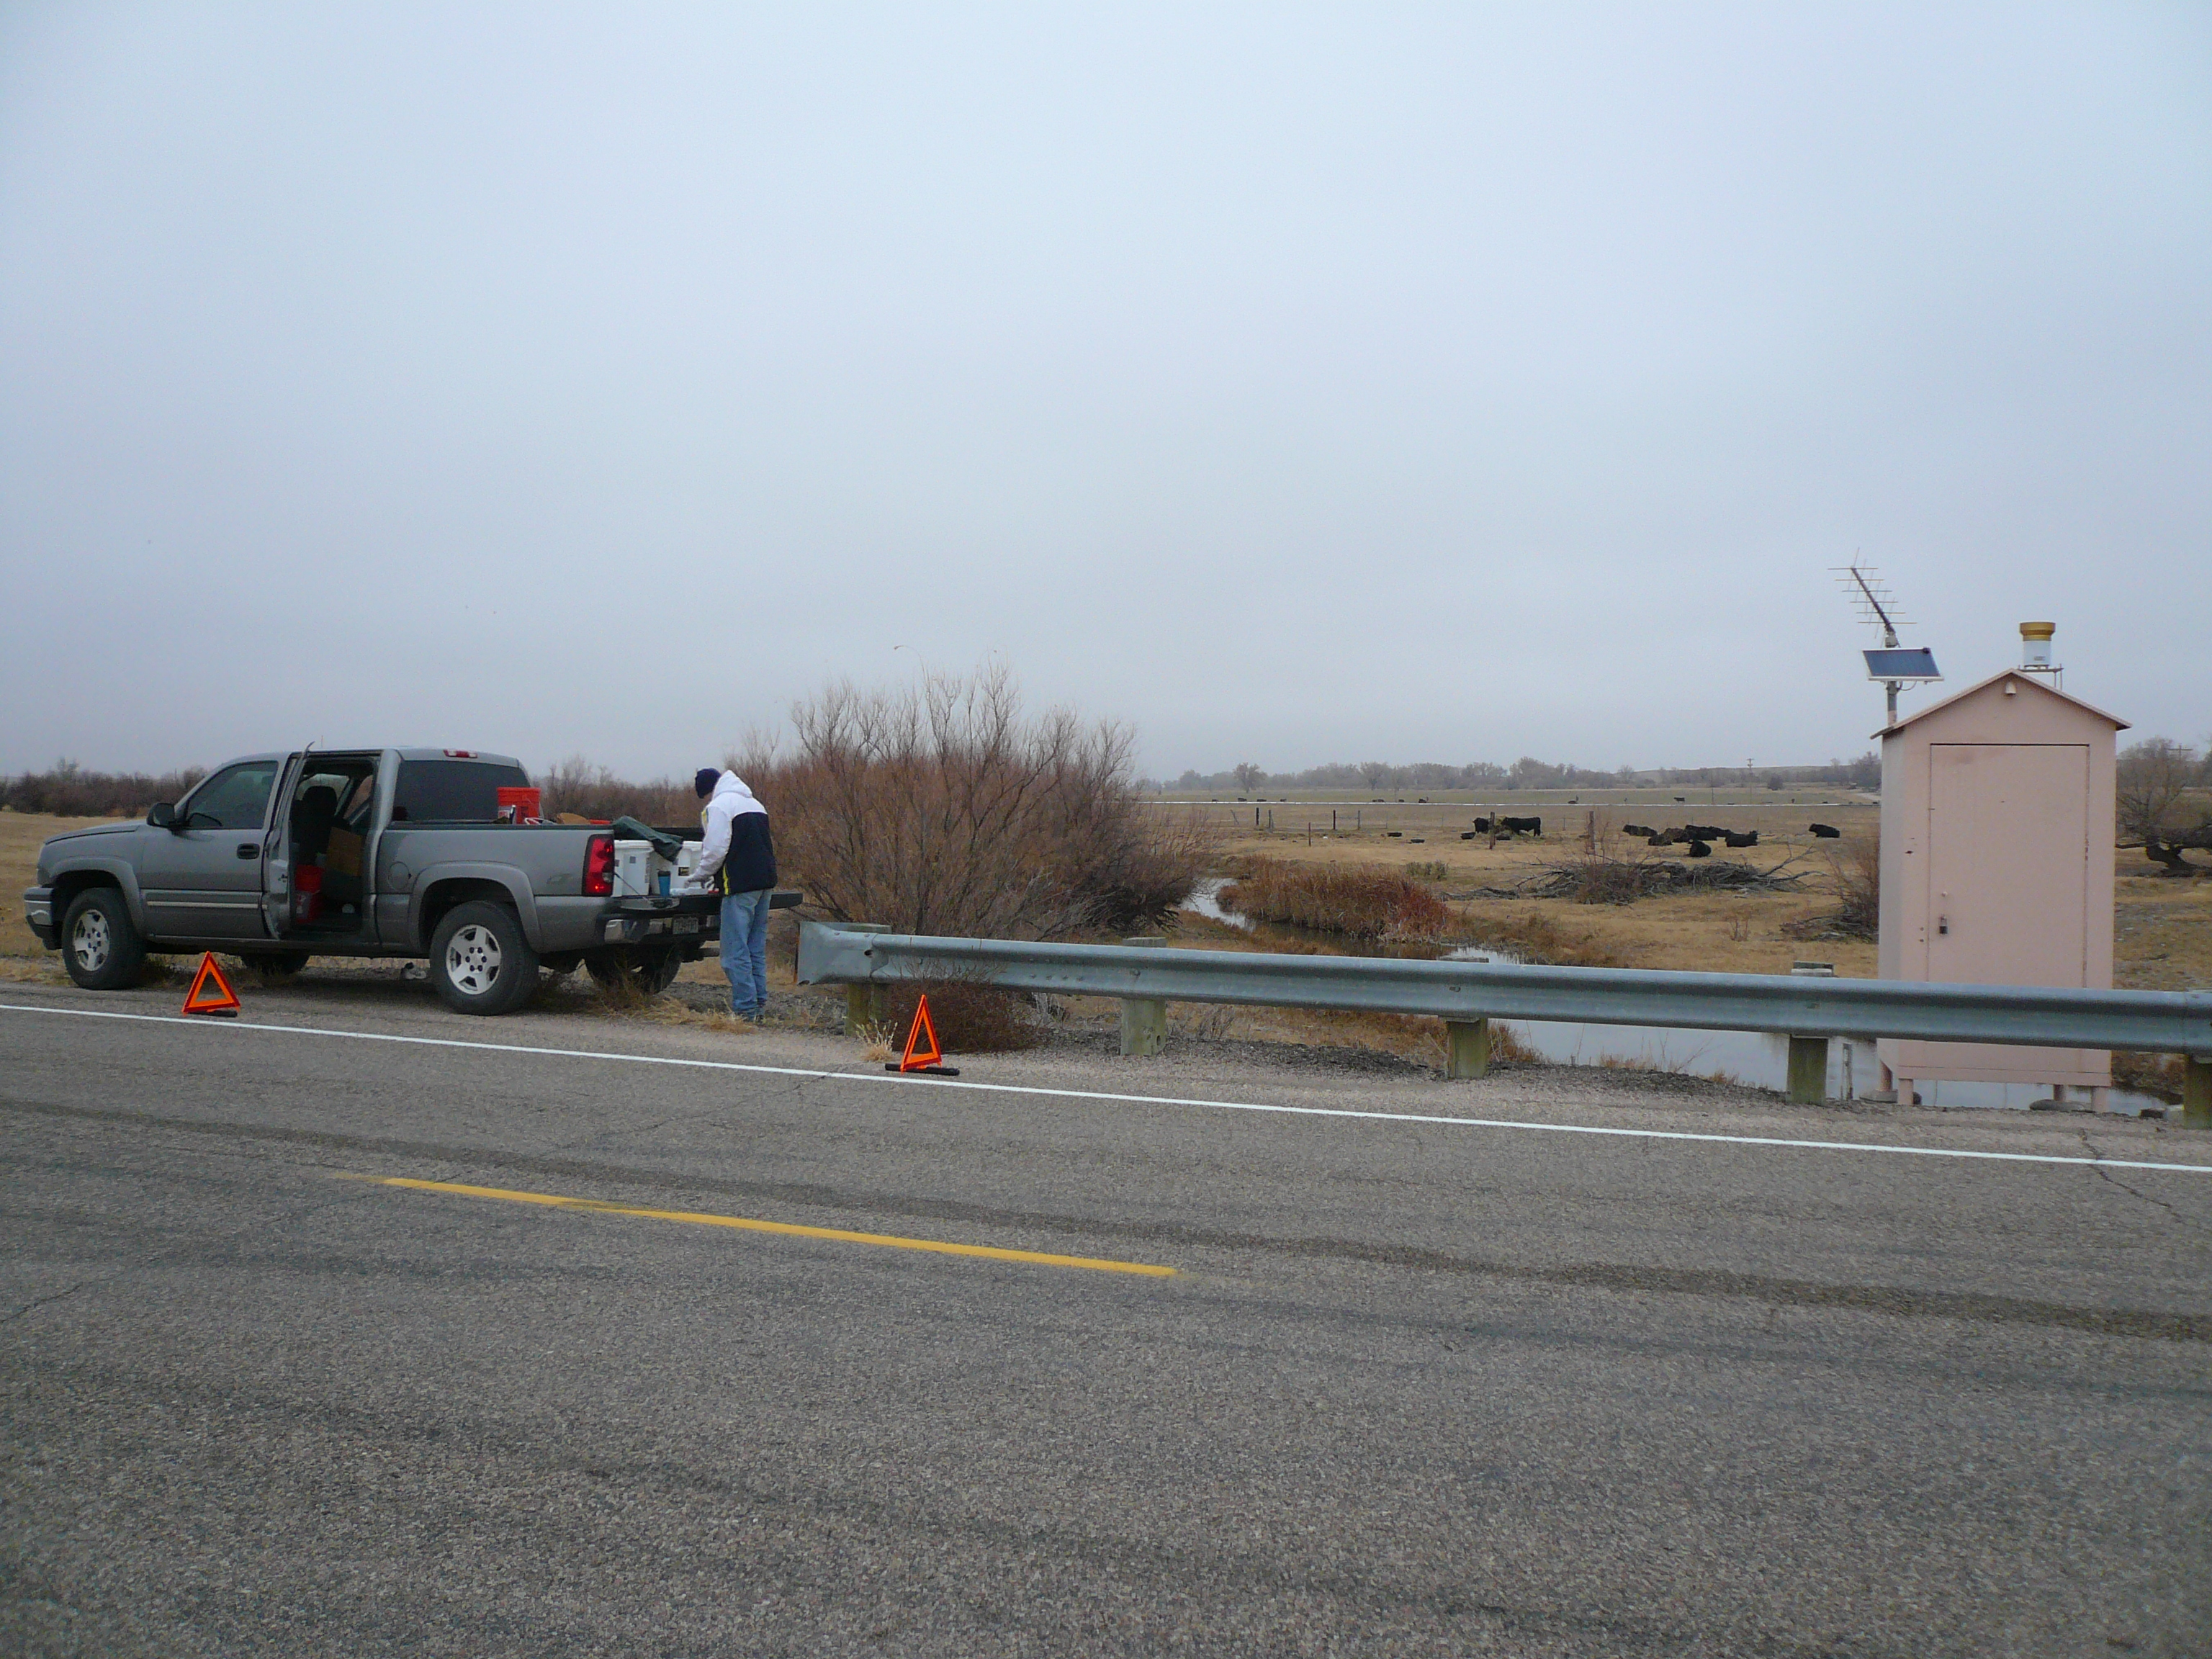
\includegraphics[width=2.9in]{Figures/Photo/GaugeSite1}
		\caption{HRC194CO.}
	\end{subfigure}%
	~
	\begin{subfigure}[t]{0.5\textwidth}
		\centering
		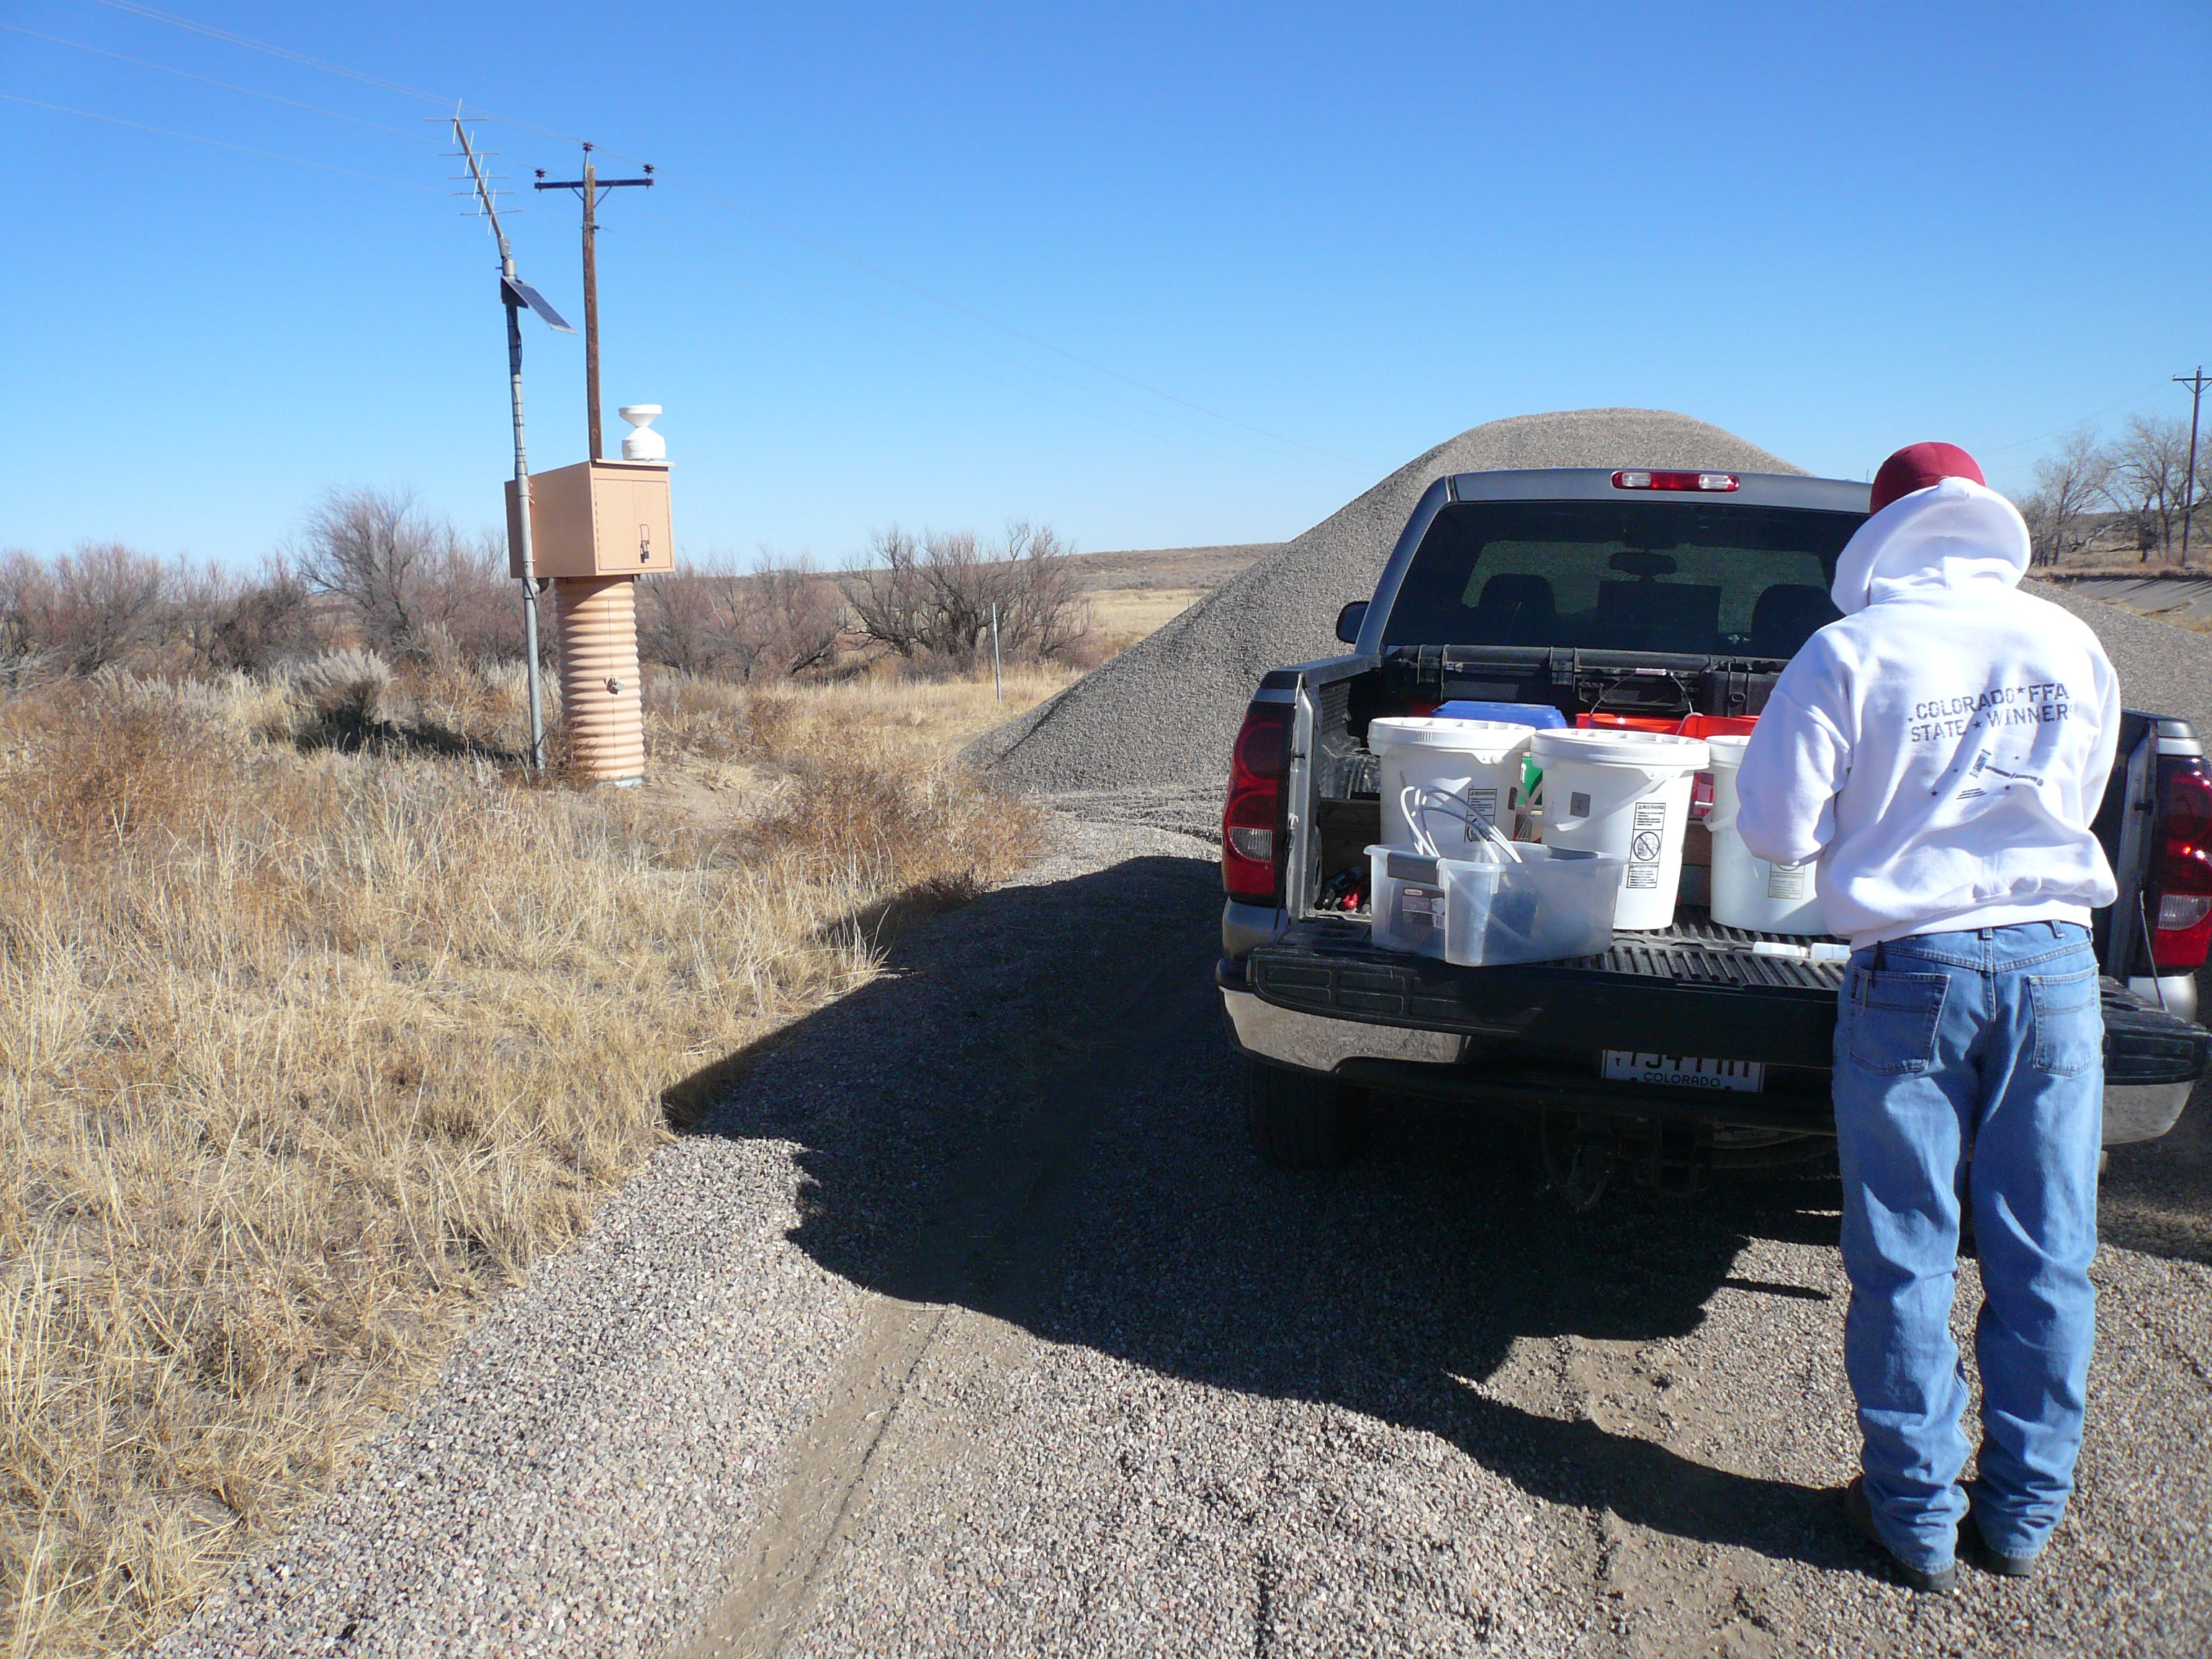
\includegraphics[width=2.9in]{Figures/Photo/GaugeSite2}
		\caption{BIGLAMCO.}
	\end{subfigure}

	\begin{subfigure}[t]{0.5\textwidth}
		\centering
		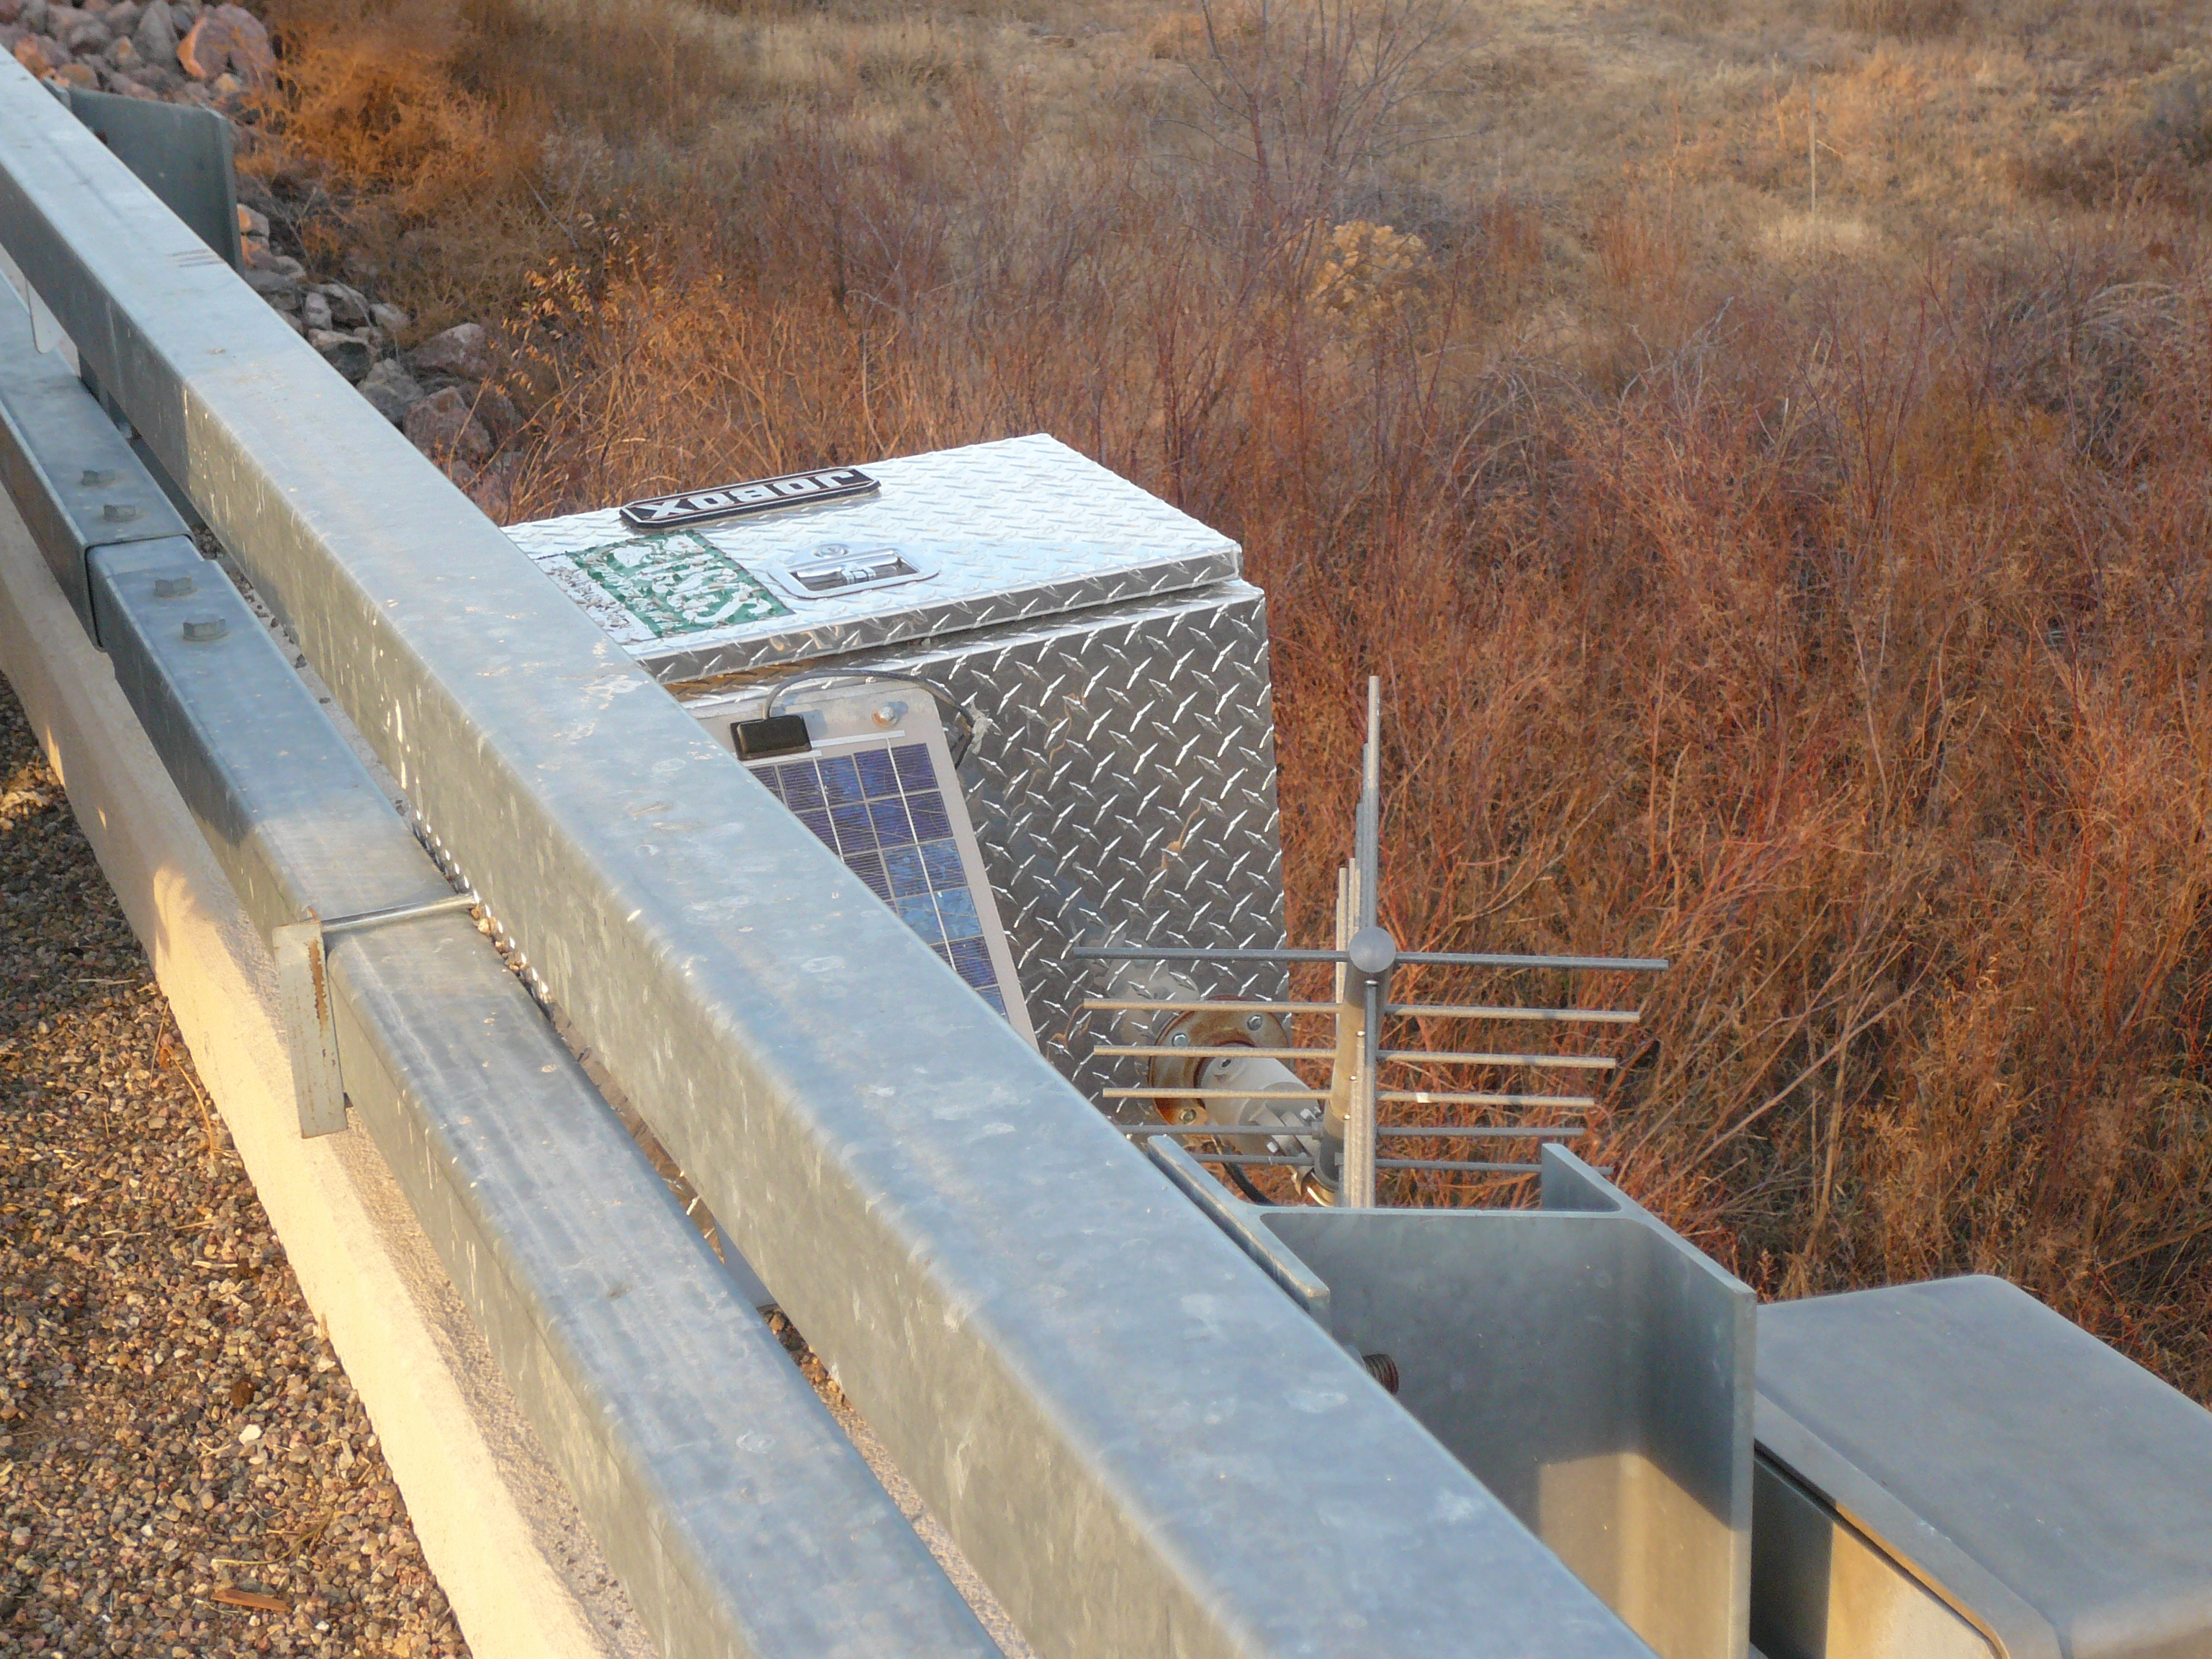
\includegraphics[width=2.9in]{Figures/Photo/GaugeSite3}
		\caption{TIMSWICO}
	\end{subfigure}%
	~
	\begin{subfigure}[t]{0.5\textwidth}
		\centering
		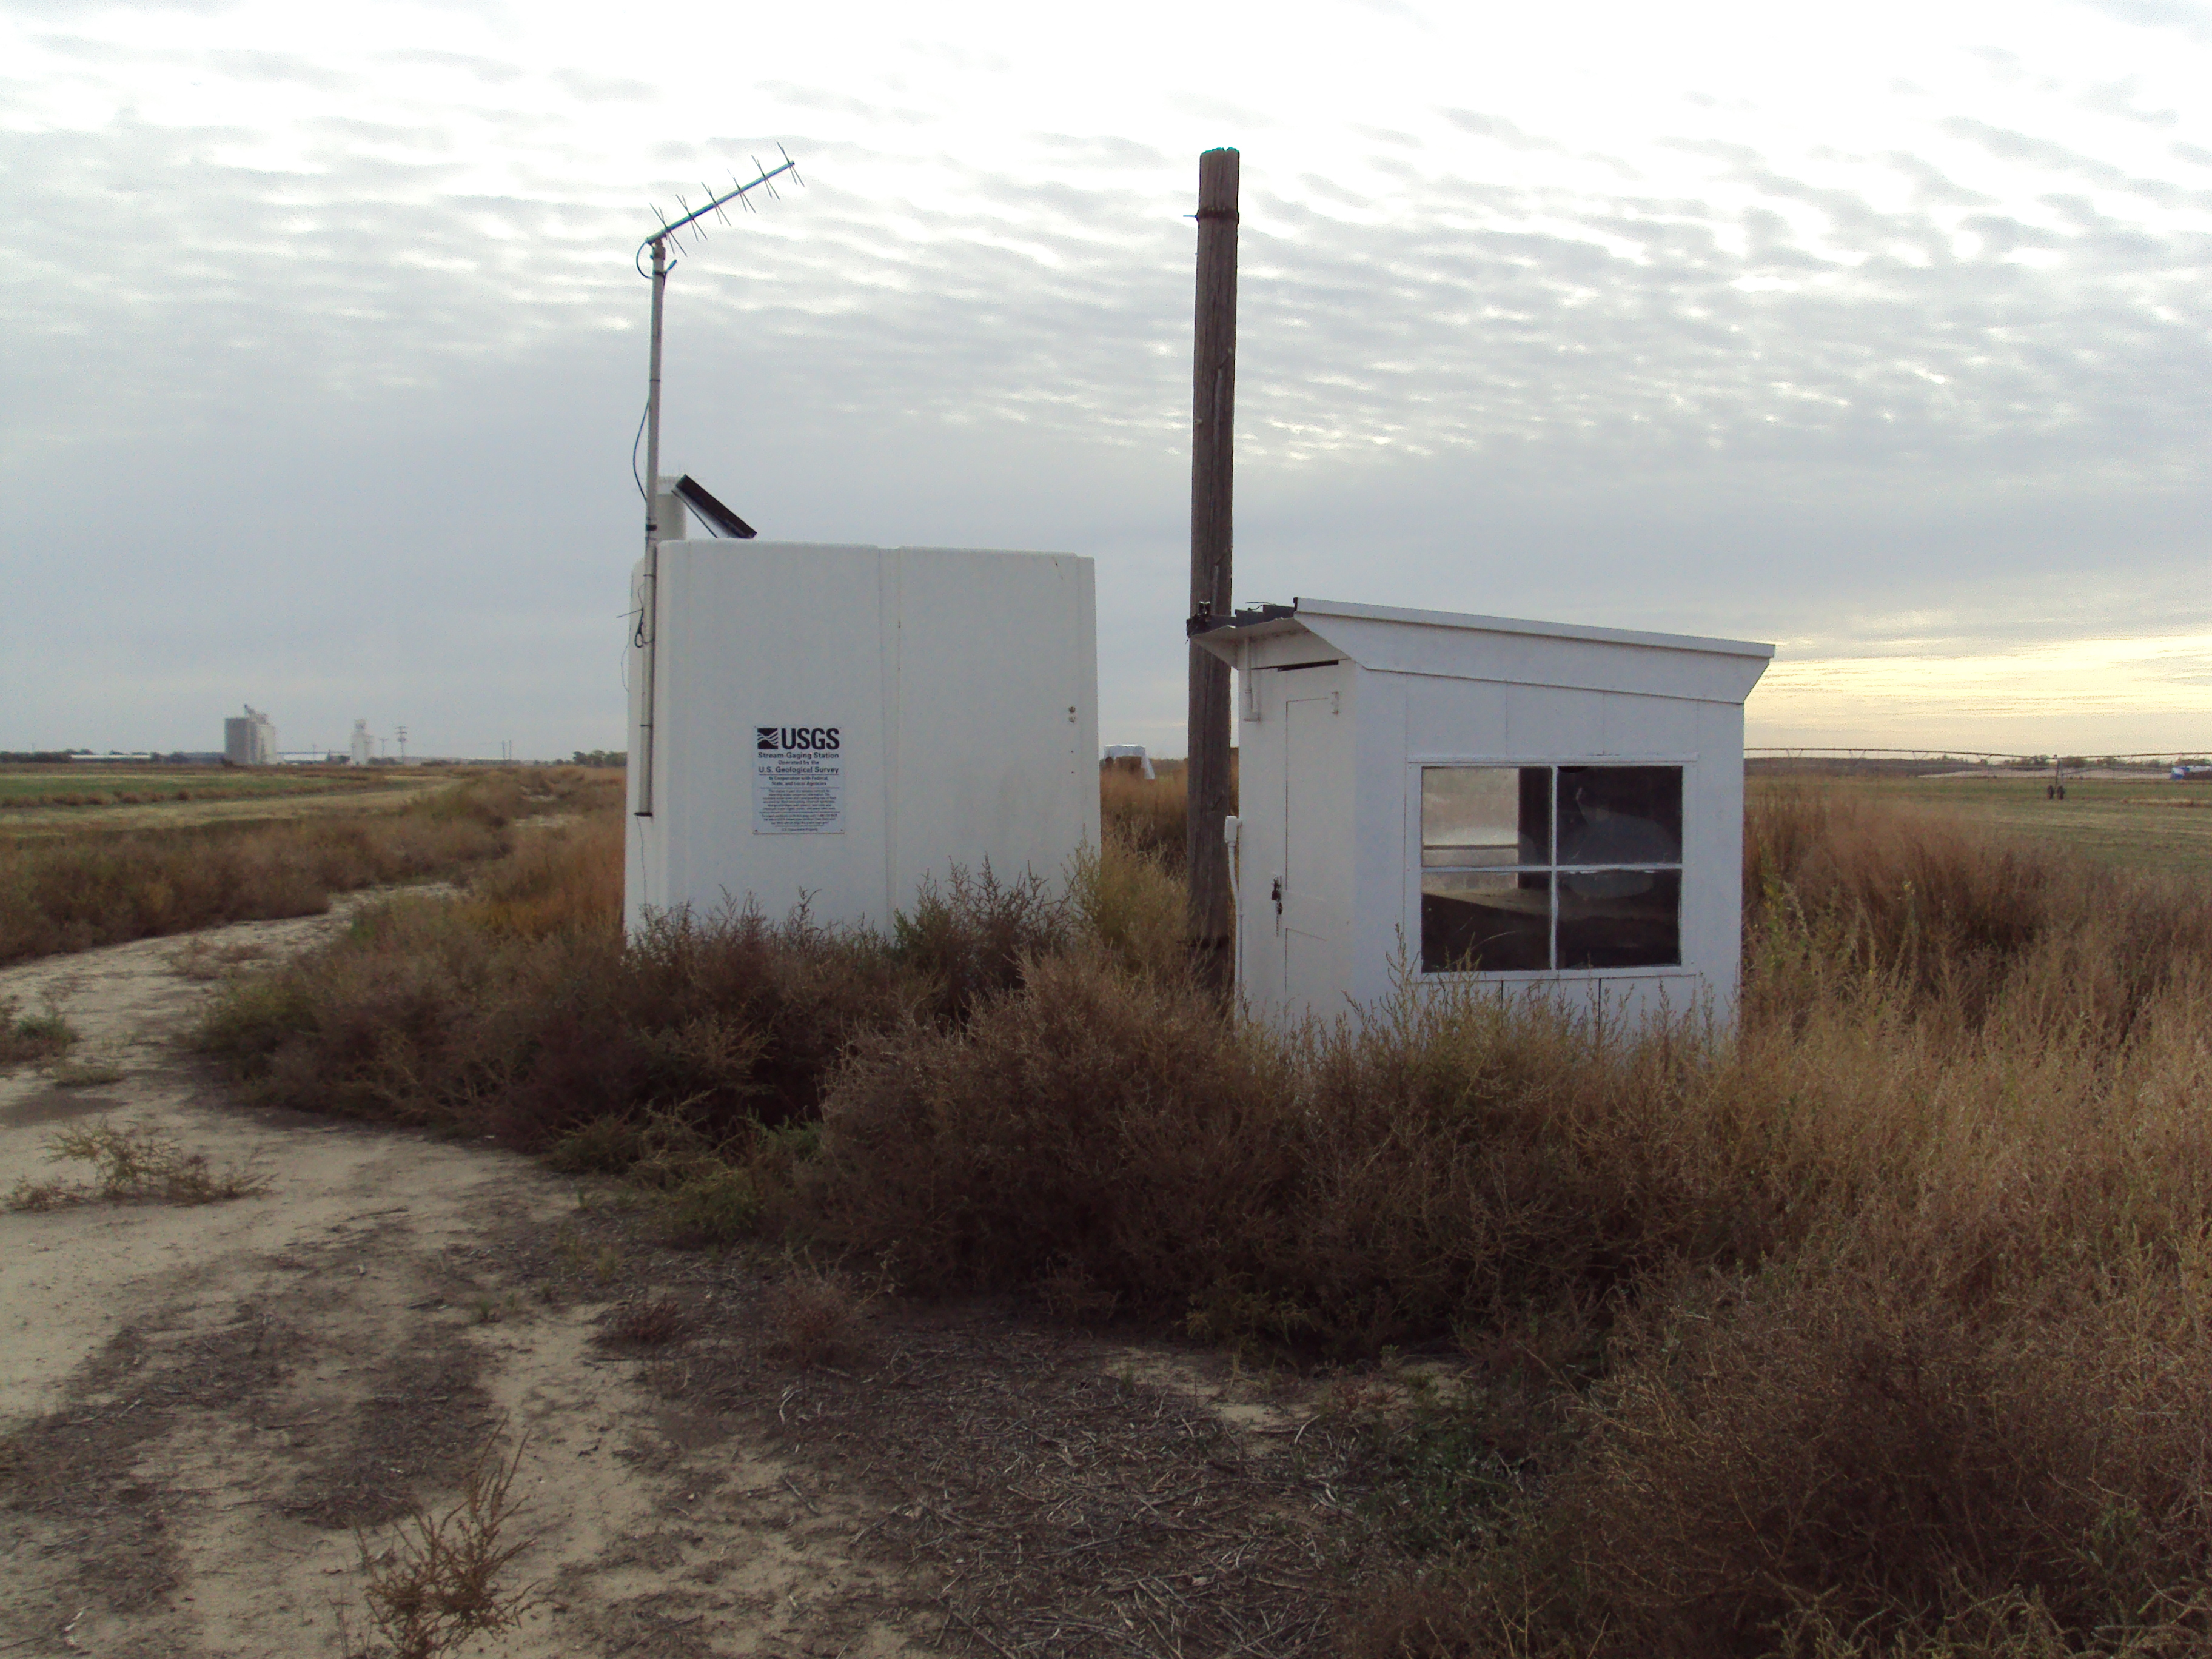
\includegraphics[width=2.9in]{Figures/Photo/GaugeSite4}
		\caption{FRODITKS}
	\end{subfigure}
	
	\begin{subfigure}[t]{0.5\textwidth}
		\centering
		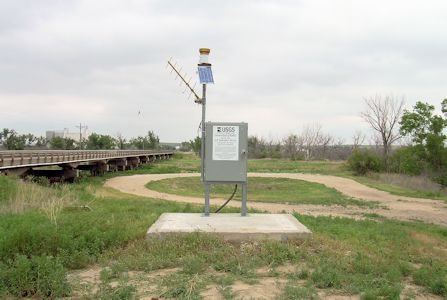
\includegraphics[width=2.9in]{Figures/Photo/GaugeSite6}
		\caption{ARKCOOKS}
	\end{subfigure}%
	\caption[Range of Stream Gauge Equipment Housings in the LARV.]{Range of Stream Gauge Equipment Housings in the LARV.}
	\label{pic:Housings}
\end{figure}

Data from the CDWR and USGS stream gauges are reported on web sites operated by the two agencies.  Table \ref{tab:gauge other data} lists the gauge sites used in this study and notes the additional data besides streamflow collected at each gauge.  Additional data are reported by the agency that owns and operates the gauge site.  USGS instruments at a CDWR gauge site are recorded and reported on the CDWR web site.  Note that the CDWR gauge site ARKLAMCO, which is owned by the USGS, does not have any additional data collection instruments.

% Table - USR stream gauge data
\begin{table}[htbp]
  \centering
  \caption[Summary of Stream Gauges with Notation of Additional Data Collected.]{Summary of Stream Gauges with Notation of Additional Data Collected.}
  \label{tab:gauge other data}
  \begin{tabular}{cccccc}
  	\toprule
  	        Study         & \multicolumn{2}{c}{Stream Gauge ID} & \multicolumn{3}{c}{Parameter} \\
  	        Reach         &   CDWR    &          USGS           & Air Temp. & Water Temp. & EC  \\ \toprule
  	\multirow{12}{*}{USR} & ARKCATCO  &                         &           &      X      &  X  \\
  	                      & HOLCANCO  &                         &           &             &  \\
  	                      & RFDMANCO  &                         &           &             &  \\
  	                      & FLSCANCO  &                         &           &             &  \\
  	                      & RFDRETCO  &                         &           &             &  \\
  	          %           & ARKROCCO  &                         &           &      X      &  X  \\
  	                      & TIMSWICO  &                         &           &             &  \\
  	                      & FLYCANCO  &                         &           &             &  \\
  	                      & CANSWKCO  &                         &           &             &  \\
  	                      & ARKLAJCO  &                         &     X     &             &  \\
  	                      & CONDITCO  &                         &           &             &  \\
  	                      & HRC194CO  &                         &           &             &  \\
  	                      & ARKLASCO  &        07124000         &           &      X      &  X  \\ \midrule
  	\multirow{7}{*}{DSR}  & ARKJMRCO  &        07130500         &           &      X      &  X  \\
  	                      & ARKLAMCO  &        07124000         &           &             &  \\
  	                      & BIGLAMCO  &                         &           &             &  \\
  	                      & BUFDITCO  &                         &           &             &  \\
  	          %           & ARKGRACO  &        07134180         &           &             &  \\
  	                      & WILDHOCO  &                         &           &             &  \\
  	                      & FRODITCKS &                         &           &             &  \\
  	                      & ARKCOOKS  &        07137500         &           &      X      &  X  \\ \bottomrule
  \end{tabular}
\end{table}

Stream flow data were obtained as average daily flow for each stream gauge. Some average daily flow records were reported as being estimated or provisional.  These data points were removed from the analysis.  Average daily flow data were quality checked for unacceptable values.  For each gauge, acceptable values were defined as those above zero and below the 99th percentile of all flows recorded at that gauge.  Unacceptable values were removed from the data set.

All stream gauges report gauge height which is the vertical distance from the gauge site datum to the water surface (Figure \ref{fig:VariableChannel}).  Gauge site datum is arbitrarily set, but is tied to a local survey benchmark.  Flow depth is the depth from the bottom of the channel to the water's surface.  While both gauge height and flow depth measure the distance to the water's surface, their datums can, and frequently do vary.  The Arkansas River is a shifting bed channel and as such, the channel bottom elevation varies with time at a gauge site.  The rating table, which is used to convert flow depth to flow rate, is configured such that flow depths below the channel bottom have a flow rate of zero.  The table is frequently updated with data obtained from routine re-calibration of the stream gauge.

% Figure - river cross section w/ variable channel bottom
\begin{figure}[htbp]
\centering
	\includegraphics[width=6in]{Figures/LineDiagram/XSectionSimple}
	\caption[Depiction of Variable Channel Bottom and Fixed Gauge Datum.]{Depiction of Variable Channel Bottom and Fixed Gauge Datum.  $ d_1 $ and $ d_2 $ are flow depths at different times.  $ h_i $ is the stream gauge height measurement at any time.}
	\label{fig:VariableChannel}
\end{figure}

Gauge height data is the directly measured value that is used to calculate flow rate.  Flow rates are calculated from gauge height using a gauge site specific rating table produced in accordance with USGS standards and procedures \citep{USGS1982a, USGS1982b}.  Gauge heights for the USGS and CDWR gauges were obtained from the respective regional offices.  Historical recorded gauge heights are not reported on web sites as these data are considered to be precursors for stream flow rate calculations.  Stream gauge data were provided as both average daily gauge height and as recorded gauge height.  Recorded gauge height is the gauge height recorded in 15-minute increments during a calendar day.  Average daily gauge height is the mean of the recorded gauge heights over a calendar day.  All gauge heights were provided in units of feet above the gauge datum.  Gauge height units were converted to SI units of meters for this study to simplify calculations and discussion.  Gauge height data were checked for accuracy by the source agency before being released to CSU staff.

Water temperature data were obtained as average daily temperature or as minimum and maximum daily temperatures, depending on the gauge site.  Average daily temperature is calculated as the mean of the minimum and maximum daily temperature.  Water temperature data were provided in units of \si{\degreeCelsius}.  Since frozen or partially-frozen river channels do not have the same gauge height to flow rate relationship as free running river channels, data corresponding to water temperatures below zero were removed from the data set.

EC data obtained from USGS and CDWR stream gauge sites were provided as average daily values for each recording gauge station.  EC values recorded at the stations were compared to available EC values measured by CSU to cross-validate both data sets.  Gauge station recorded EC values were quality controlled by removing the bottom and top 1\% of EC values for each gauge.  Changes in average daily EC between consecutive days were checked for validity.  Changes greater than 33\% were analyzed to determine if the EC change was valid.  The average daily flow rate and time of year were taken into consideration when determining if the questionable EC values were valid.  EC values that exceeded the 33\% change but were accompanied by large changes in EC or during peak irrigation seasons were considered valid EC values.  Values considered to be invalid were removed from the data set.  EC values were provided in units of \si{\micro\siemens\per\centi\meter}.

Atmospheric data was required to determine the volume of water evaporated from the river's surface.  The Colorado Agricultural Meteorological Network (CoAgMet) was chosen as the source for atmospheric data.  The National Weather Service station sites in the study regions are located in populated areas or at airports and is only suitable for weather analysis.  CoAgMet station sites are more numerous, are located in agricultural areas, and are suitably equipped for evaporation and transpiration ($ET$) analysis.  An example of one of the weather stations is shown in Figure \ref{pic:CoAgMetStation}.  The CoAgMet network is operated by the Colorado Climate Center at CSU and consists of 86 weather stations throughout the state.  Some stations are only seasonally operational \citep{Andales2009, Csu2012}.  Of the full-time sites, three are located in the USR and three are located in the DSR as shown in Figures \ref{map:USRCoAgMetLocations} and \ref{map:DSRCoAgMetLocations}, respectively. The CoAgMet weather stations in the USR are located such that they represent the upper, middle, and lower segments of the USR.  The CoAgMet stations in the DSR are more tightly grouped toward the upstream end of the reach, but still are considered representative of the study reach. The weather stations are primarily located in agricultural areas to provide agricultural researchers with data used for many different research applications.  The data also are available to the public through a web site.  This has aided farmers in determining irrigation timing and quantity \citep{Andales2009}.  Table \ref{tab:CoAgMetInstruments} is a list of the parameters measured at the CoAgMet stations and the typical instruments used.  Not all stations are identical.  Instruments were replaced or upgraded by CCC staff when required with instruments that were available and equal to or better in quality than the instrument being replaced.

% Picture - CoAgMet weather station
\begin{figure}[htbp]
\centering
	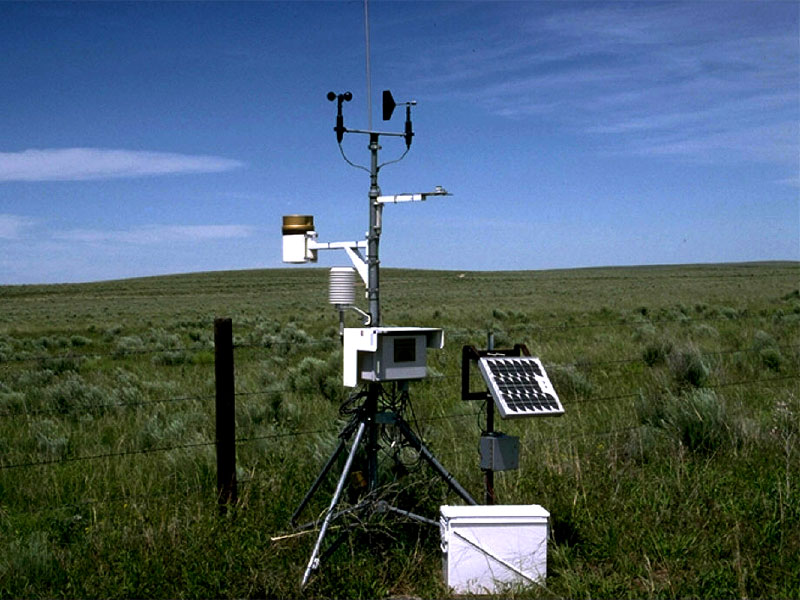
\includegraphics[width=4in]{Figures/Photo/CoagmetStation}
	\caption[Typical CoAgMet Weather Station.]{Typical CoAgMet Weather Station.}
	\label{pic:CoAgMetStation}
\end{figure}


% Map - USR CoAgMet weather station locations
	\begin{landscape}
	\begin{figure}[htbp]
		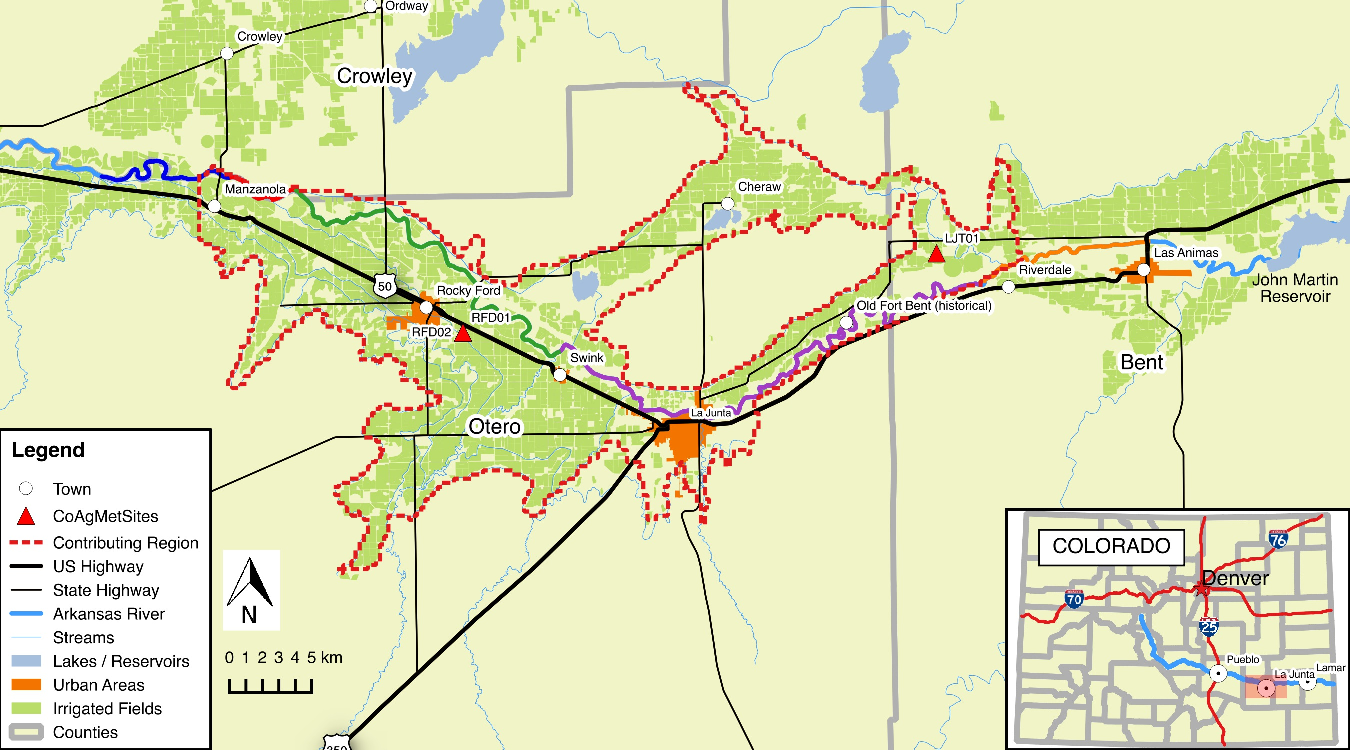
\includegraphics[scale=1]{Figures/Map/USRCoAgMet}
		\caption[USR CoAgMet Weather Station Locations.]{USR CoAgMet Weather Station Locations.}
		\label{map:USRCoAgMetLocations}	
	\end{figure}
	\end{landscape}

% Map - DSR CoAgMet weather station locations
	\begin{landscape}
	\begin{figure}[htbp]
		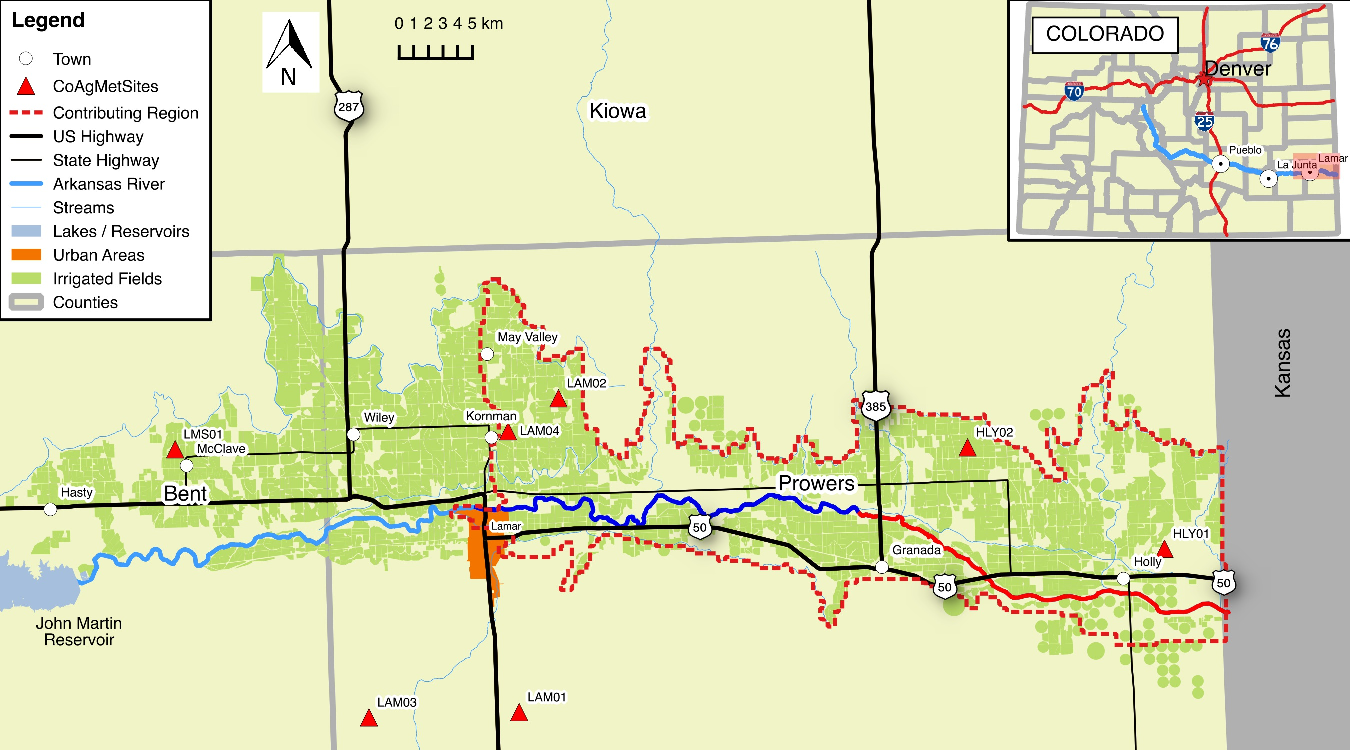
\includegraphics[scale=1]{Figures/Map/DSRCoAgMet}
		\caption[DSR CoAgMet Weather Station Locations.]{DSR CoAgMet Weather Station Locations.}
		\label{map:DSRCoAgMetLocations}	
	\end{figure}
	\end{landscape}
 
% Table - Typical instruments at CoAgMet station
\begin{table}[htbp]
\centering
\caption[Typical Instrumentation at CoAgMet Weather Stations.]{Typical Instrumentation at CoAgMet Weather Stations.}
\label{tab:CoAgMetInstruments}
\begin{tabular}{c c}
	\toprule
	       Measured Parameter        & Typical Instrument                          \\ \toprule
	Temperature \& Relative Humidity & Vaisala HMP45C Probe                        \\
	              Wind               & R.M. Young Wind Sentry                      \\
	        Solar Radiation          & Licor LI-200X Pyranometer                   \\
	         Precipitation           & TE525 tipping bucket raingauge              \\
	        Soil Temperature         & CSI Model 107 Soil Temp Probe (thermistor)  \\
	          Data Loggers           & Campbell Scientific CR10, CR10X, and CR1000 \\ \bottomrule
\end{tabular}
\end{table}

Table \ref{tab:CoAgMet} lists the weather stations in the LARV that were used in this study.  This table lists the station name and location, the state of irrigation of the land surrounding the site, the date of first record, and a comparative estimate of the site estimated $ET_{ref}$ to the actual $ET_{ref}$.  The irrigation state of the land surrounding the site is used to determine the comparative estimate of the site estimated $ET_{ref}$ to the actual  $ET_{ref}$.  If the monitoring station is on irrigated land then the $ET_{ref}$ values calculated based on site data are expected to be at or near the actual value of $ET_{ref}$ for the site.  If the station is on dry, or non-irrigated land, then calculated $ET_{ref}$ values tend to over estimate the actual $ET_{ref}$.

% Table - CoAgMet stations used in analysis
\begin{table}[htb]
  \centering
  \caption[CoAgMet Weather Stations used for analysis in the LARV.]{CoAgMet Weather Stations used for analysis in the LARV.}
  \label{tab:CoAgMet}
    \begin{tabular}{ccccccc}
    	\toprule
    	                         &                           &                                &                &                             &                                 &        Comparative        \\
    	         Study           &                        \multicolumn{3}{c}{Station }                         & \multirow{2}{*}{Irrigation} &             Date of             &          Est. of          \\
    	\cmidrule{2-4}
    Reach &            ID             &              Name              &    Location    &                             &          First Record           &          Site ET          \\ \toprule
    	\multirow{7}[0]{*}{USR}  & \multirow{2}[0]{*}{FWL01} &   \multirow{2}[0]{*}{Fowler}   &  Fowler Golf   &  \multirow{2}[0]{*}{Full}   & \multirow{2}[0]{*}{17 Mar 2005} &  \multirow{2}[0]{*}{--}   \\
    	                         &                           &                                &     Course     &                             &                                 &  \\
    	     \cmidrule{2-7}      & \multirow{2}[0]{*}{LJT01} &  \multirow{2}[0]{*}{LaJunta}   &    11 mi NE    &  \multirow{2}[0]{*}{Full}   & \multirow{2}[0]{*}{17 Mar 2005} & \multirow{2}[0]{*}{Under} \\
    	                         &                           &                                &   of LaJunta   &                             &                                 &  \\
    	     \cmidrule{2-7}      & \multirow{3}[0]{*}{RFD01} & \multirow{3}[0]{*}{RockyFord}  & CSU Experiment &  \multirow{3}[0]{*}{Full}   & \multirow{3}[0]{*}{6 Apr 1992}  &  \multirow{3}[0]{*}{--}   \\
    	                         &                           &                                & Station, Rocky &                             &                                 &  \\
    	                         &                           &                                &      Ford      &                             &                                 &  \\ \toprule
    	\multirow{6}[0]{*}{DSR}  & \multirow{2}[0]{*}{HLY01} &   \multirow{2}[0]{*}{Holly}    &    5 mi NW     &  \multirow{2}[0]{*}{Part}   & \multirow{2}[0]{*}{27 Sep 2001} & \multirow{2}[0]{*}{Over}  \\
    	                         &                           &                                &    of Holly    &                             &                                 &  \\
    	     \cmidrule{2-7}      & \multirow{2}[0]{*}{HLY02} & \multirow{2}[0]{*}{Holly \#2}  &   8.5 mi NW    &  \multirow{2}[0]{*}{Full}   & \multirow{2}[0]{*}{21 May 2005} &  \multirow{2}[0]{*}{--}   \\
    	                         &                           &                                &    of Holly    &                             &                                 &  \\
    	    \cmidrule{2-7}
%     & \multirow{2}[0]{*}{LAM01} & \multirow{2}[0]{*}{Lamar \#1}  &    4.5 mi S    &   \multirow{2}[0]{*}{Dry}   & \multirow{2}[0]{*}{3 Aug 1996}  & \multirow{2}[0]{*}{Over}  \\
    	           %             &                           &                                &    of Lamar    &                             &                                 &  \\
    	    \cmidrule{2-7}
%     & \multirow{2}[0]{*}{LAM03} & \multirow{2}[0]{*}{Lamar \#3}  &    10 mi SW    &   \multirow{2}[0]{*}{Dry}   & \multirow{2}[0]{*}{31 Jul 2002} & \multirow{2}[0]{*}{Over}  \\
    	           %             &                           &                                &    of Lamar    &                             &                                 &  \\
    	     \cmidrule{2-7}      & \multirow{2}[0]{*}{LAM04} & \multirow{2}[0]{*}{Lamar \#4}  &   4.5 mi NNE   &  \multirow{2}[0]{*}{Full}   & \multirow{2}[0]{*}{11 May 2005} &  \multirow{2}[0]{*}{--}   \\
    	                         &                           &                                &    of Lamar    &                             &                                 &  \\
    	   %\cmidrule{2-7}
%     & \multirow{2}[0]{*}{LMS01} & \multirow{2}[0]{*}{Las Animas} &    1 mi NW     &  \multirow{2}[0]{*}{Full}   & \multirow{2}[0]{*}{17 Mar 2012} &  \multirow{2}[0]{*}{--}   \\
    	           %             &                           &                                &   of McClave   &                             &                                 &  \\ \bottomrule
    \end{tabular}
\end{table}

CoAgMet provides both raw weather data from all weather stations and daily $ET_{ref}$ values calculated for select stations.  Daily $ET_{ref}$ values were obtained from the sites in the LARV.  The American Society of Civil Engineers (ASCE) Environmental and Water Resources Institute (EWRI) standardized tall crop evapotranspiration reference Penman-Monteith equation was used by the Colorado Climate Center to calculate $ET_{ref}$.  Values are obtained in units of \si{\milli\meter\per\day}.  

The average daily $ET_{ref}$ for a region surounding a study reach was calculated as the mean of the stations reporting $ET_{ref}$ for a given day. If a station or group of stations did not have data for a particular day in the study time frame, then then those stations were not included in the calculation.  An assumption was made that the $ET_{ref}$ over the Arkansas River within a study reach could be approximated as the mean of the reported values within the surrounding region.

The minimum daily relative humidity ($RH_{min}$) and wind speed at \SI{2}{\meter} above ground surface ($u_2$) data were obtained from the same CoAgMet stations as the precipitation and $ET_{ref}$ data.  $RH_{min}$ values were reported as a fraction and values less than zero were removed from the data set.  Wind speed values were reported as wind run, which is the total distance the air traveled during the calendar day and is reported in units of \si{\kilo\meter\per\day}.  A small number of the wind run values in the obtained data set were less than zero and were removed.  Historical average wind run values were not available to provide a method to sanitize the wind run upper bound values.  Wind run values were converted to average daily wind speed in units of \si{\meter\per\second}.

Precipitation data were collected from the same network of monitoring stations used to generate average daily $ET_{ref}$ as daily values in units of \si{\milli\meter\per\day}.  Data was not sanitized before publication to the CoAgMet web site.  A small number of total daily precipitation values in the obtained data set were less than zero or exceeded reasonable maximum values.   Daily total precipitation values less than zero or greater than 1.5 times the highest average precipitation reported by the National Weather Service were excluded.  As with the $ET_{ref}$ data, the mean precipitation value over the surrounding region of a study reach for any given day only included those stations reporting data.  Any additional data collected from the CoAgMet system was treated in a similar manner.
\clearpage{}

\end{linenumbers}
% !TeX root = CH04-WaterBalanceModel.tex
% !TeX spellcheck = en_US
% !TeX encoding = UTF-8
\renewcommand{\thechapter}{4}
\chapter{Evaluation of NPS Return Flow to the River Using a Water Balance Model}
\label{chap:WaterBalanceModel}

\begin{linenumbers}
\section{Water Balance Model Applied to the LARV}
\label{sec:AppliedWaterModel}

The purpose of the water balance model is to determine the volume of unaccounted for water in each reach.  We begin with a basic water balance model as describe in most hydrology texts --- \parencite{wanielista1997}.
\begin{equation}
	\textnormal{change in storage = inputs - outputs} \nonumber
\end{equation}

Adding the variables, both known and unknown, present in the LARV we have the following equation:
\begin{equation}
\label{eq:water1}
	\frac{\Delta S}{\Delta t} = Q_{in,US} + \sum Q_{in} + P + R + B - Q_{out,DS} - \sum Q_{out} - E - T - F + X
\end{equation}
\begin{longtable}{r p{5.5in}}
	Where: \\
	$\displaystyle \frac{\Delta S}{\Delta t}$ =&Stored volume change between time steps.\\
	$ Q_{in,US} $ = & Flow in the river entering the study reach at the upstream end.\\
	$ \displaystyle \sum Q_{in} $ = & Flow gained by the river from tributaries and other gauged sources.\\
	$ P $ = & Volume of water gained to the river due to precipitation falling directly on the river's surface.\\
	$ R $ = & Volume of water gained to the river due to precipitation runoff from adjacent land. \\
	$ B $ = & Volume of water gained to the river due to subsurface flow. \\
	$ Q_{out,DS} $ = & Flow in the river leaving the study reach at the downstream end.\\
	$ \displaystyle \sum Q_{out} $ & Flow lost from the river to canals and other gauged sinks.\\
	$ E $ = & Volume of water lost from the river due to direct evaporation from the water's surface.\\
	$ T $ = & Volume of water lost from the river due to plant transpiration.\\
	$ F $ = & Volume of water lost from the river due to infiltration into the subsurface flow.\\
	$ X $ = & Water volume gains and losses to/from unknown sources and sinks.\\
\end{longtable}

The inclusion of the $ X $ term signifies one of two types of unknown values addressed in this thesis.  There are known unknowns, which are directly addressed and unknown unknowns.  Known unknowns are those values or terms which are known to exist, but the magnitude and sign of their effect is unknown and/or immeasurable.  Unknown  unknowns are those values or terms which we do not know exist.  Their existence and effect on a system are yet to be discovered.  We assume with the current state of chemistry and physics, that the $ X $ term is insignificant.  However, we cannot discount it from our analysis.

If we combine the terms that are unknown or unmeasured, we arrive at the following equation:
\begin{equation}
	\label{eq:water01}
	\frac{\Delta S}{\Delta t} = Q_{in,US} + \sum Q_{in} + P - Q_{out,DS} - \sum Q_{out} - E + Q_{UNPS}
\end{equation}
\begin{tabular}{r p{5.5in}}
	Where: \\
	\Qnps = & The sum of gains from non-point sources and losses to non-point sinks \\
		= &$ Q_{UNPS} = R + B - T - F + Q_{U,in} - Q_{U,out} +X $.\\ 
\end{tabular}\\

%\emph{III - define $Q_U$ constituents}\\
There is no reasonable method for differentiating the components of \Qnps, therefore the abbreviation NPS in this thesis refers to both non-point sources and non-point sinks.   \Qnps includes the non-point source gains from groundwater sources($ B $), non-point source losses to groundwater sinks {}$ F $), transpiration losses from plants in the river channel ($ T $), and gains from precipitation runoff from adjacent land ($ R $).  Additionally, this term includes ungauged flows leaving and entering the river.  Ungauged gains to the river ($ Q_{U,in} $) are suspected to be primarily in the form of irrigation drainage from adjacent farmland.  Other sources could be due to errors in underestimating flows entering the river or overestimating flows leaving the river.  Ungauged losses from the river ($ Q_{U,out} $) are suspected to be primarily in the form of minor or unauthorized withdrawals from the river channel.  Of the ungauged flows, irrigation drainage from adjacent farmlands is assumed to be the largest contributor.

The two groundwater components of \Qnps are suspected of being the largest components of \Qnps.  Water transfer between the aquifer and river happens continually whereas $ Q_{U,in} $, $ Q_{U,out} $, $ R $, and $ T $ are not continuous.  $ Q_{U,in} $ and $ Q_{U,out} $ only occur periodically when individuals actively withdraw from the river or allow irrigation runoff to return to the river.  $ R $ only occurs during rain events.  Within the LARV, most rainwater is captured in irrigation canals.  Only precipitation falling in the riparian zone is likely to reach the river.  $ T $ only occurs during growing season.  This value is also only considering the transpiration happening within the river channel and does not include the riparian zone.  Any losses due to transpiration in the riparian zone are first considered river losses to the aquifer ($ F $).

Re-arranging equation \eqref{eq:water01} to solve for the unknown values produces equation \ref{water02}.  Due to the nearly identical method of calculating flow ($ Q $) and it's associated error and uncertainty, these terms were associated with each other.  Likewise, the precipitation ($ P $) and evaporation ($ E $) terms were associated with each other.
\begin{equation}
	\label{eq:water2}
	Q_{UNPS} = \left( Q_{out,DS} + \sum Q_{out} - Q_{in,US} - \sum Q_{in} \right) + \frac{\Delta S}{\Delta t} - \left( P + E \right)\\ 
\end{equation}

This model is further simplified to Equation \ref{eq:water3} which combines terms that are calculated using similar methods to facilitate discussion.
\begin{equation}
	\label{eq:water3}
	Q_{UNPS} = \frac{\Delta S}{\Delta t} - \sum Q_{Total} - \sum Q_{Atm}\\ 
\end{equation}
\begin{tabular}{r p{5.5in}}
	Where:&\\
	$ \displaystyle \frac{\Delta S}{\Delta t} $ = & Reach storage change per time-step.\\
	$ \displaystyle \sum Q_{Total} $ = & $ Q_{in,DS} + \sum Q_{in} - Q_{out,US} - \sum Q_{out} $ = Sum of flows added and removed \\
		& from the reach per time-step. \\
	$ Q_{Atm} $ = & $ P - E $ = The sum of precipitation gains and evaporation losses, per time \\
		& step.\\
\end{tabular}\\

A time step of one day was established for all models calculated in this thesis.  Most of the data from agencies is readily available in average daily format.  While most of the data could also be obtained in hourly or quarter-hourly format, it was assumed that the additional information would not improve model accuracy.

\clearpage{}
\section{Stochastic and Deterministic Models}
\label{sec:StochAndDetermModels}

Deterministic and stochastic models are used in both the unaccounted for water and mass balance models.  Deterministic models are fully determined by the input parameters or variables.  Randomness of any kind is not included.  Stochastic models extend deterministic models by including one or more random parameters.  Given the same input parameter values, a stochastic model will produce different results with each iteration.

There are many recognized methods for solving stochastic models.  Solutions to these models are not definite and the term "solve" must be taken loosely.  Any individual solution from a stochastic model is one of a potentially infinite number of possible solutions.  The Monte Carlo (MC) simulation technique was used to obtain solutions for all stochastic models in this thesis.  The MC technique is conceptually simple.  The stochastic model is repetitively solved in a series of iterations.  The combined solutions from all iterations are used to define the solution statistics of the model.  

The number of iterations performed is determined by calculating and analyzing a set of identifier statistic(s) after each run.  Identifier statistic(s) are those that the modeler has determined to be of value in determining when to terminate the model.  These statistics are monitored to identify when the change in the statistic has reached a predetermined threshold.  It was determined that for the sake of simplicity, all of the models calculated in this thesis would use the same number of iterations.  The USR mass balance model is the most complex model as it has the largest number of input variables and uncertainty terms.  The identifier statistics used were the mean, variance, and skewness which are the first, second, and third moments of the probability density.  These were calculated for each iteration.  The threshold between the observed iteration and the previous iteration was fixed at 0.1\%.  The identifier statistics reached the threshold in the following order: mean, variance, and skewness.  Skewness reached its break point shortly before the 500th iteration.  A judgment call was made to increase the factor of safety.  Therefore, the number of stochastic model iterations was fixed at 5,000.  The fourth moment, kurtosis, was also calculated and analyzed for each iteration.  It was found to be too sensitive as it did not consistently stay within the accepted cutoff threshold of 0.1\%.  It is assumed that this sensitivity is due to the existence of a significant number of outliers that cause the distribution of results to be non-normal.

\section{Error and Uncertainty.}
\label{sec:ErrorAndUncertainty}

Any problem that measures variable natural processes must account for parameter and model uncertainties \parencite{vicens1975}.  Parameter uncertainty is derived from measurement error, spatial variability, and temporal variability \parencite{herschy2002}.  Measurement error is the difference between the true and measured values.  Most of this error type is due to instrument measurement inaccuracies due to either error inherent in the instrument or from errors in calibration or measurement.  Measurement errors inherent to the instrument are uncorrectable and cannot be accounted for within the model.  Errors due to calibration or measurement deviations are only correctable at the time of measurement or calibration and cannot be accounted for within the model.

Spatial variability is the difference in the true value at different points when measured at the same time.  Data collected at a single given point in space may not be representative of the area it is assumed to represent due to spatial variability.  This can manifest itself even with very small distances between measurements.  Temporal variability is the difference in the true value at the same point, but at different times.  Data collected at a one time may not be representative of the time frame it is assumed to represent due to temporal variability \parencite{Gates1996}.  Again, this can be manifested even over small time differences.  Due to instrument error, the spatiotemporal variability of the measured object, and the inability to know the true value of the measurement, reported parameter values should be treated as random variables \parencite{haan1989,haan2002}.

Almost all of the data was obtained from outside agencies and was not collected by the research team.  These agencies have data uncertainty ranges that account for all parameter uncertainties.  These uncertainties are expressed in accordance with the ISO Guide to Expression of Uncertainty in Measurement (GUM) \parencite{gum2008}.  While the GUM classifies uncertainty as either "Type A" or "Type B", the all of the data included in this thesis has uncertainty evaluations described as "Type B".  Type B evaluations usually use standard deviations and assumed probability distributions obtained from scientific judgment, available information, and possible variability of a measurement.

The data originators have provided uncertainty ranges which include instrument measurement random error and uncertainties due to temporal variations of the measured location.  The root mean square method is used to estimate the uncertainty related to measurement of water quantity and water quality values \parencite{harmel2007, gum2008}.  \textcite{harmel2007} describe this measurement uncertainty as the “probably error range”, and quantify upper and lower uncertainty boundaries for measured data points as the following when attempting to specify an expected range of expected values.
\begin{align}
	\sigma^2 = \left( \frac{O_i-UO_{i}(l)}{3.9} \right)^2  &  \phantom{xxxxxxxx} or  & 	\sigma^2 = \left( \frac{UO_{i}(u)-O_i}{3.9} \right)^2 \label{eq:uncertainty1}
\end{align}
\begin{tabular}{r p{5.5in}}
	Where:\\
	$ \sigma^2 $ = & variance about measured data value $ O_i $.\\
	$ O_i $ = & measured value.\\
	$ UO_i $ = & upper $ (u) $ and lower $ (l) $ uncertainty boundaries.\\
	$ 3.9 $ = & number of standard deviations accounting for $ >99.99 $\% of a normal probability distribution
\end{tabular}\\

The data collected for this thesis is assumed to represent the mean of a normal distribution of possible values.  The upper and lower bounds of the distributions are given as either a percent or value deviation from the mean.  Equation \ref{eq:uncertainty1} is re-written from the definition found in \textcite{harmel2007} to that found in equation \ref{eq:uncertainty2}.
\begin{align}
	\sigma^2 = \left( \frac{\mu - (\mu - \mu p)}{3.9} \right)^2  &  \phantom{wordsssssss} or \phantom{s}  & 	\sigma^2 = \left( \frac{(\mu + \mu p) - \mu}{3.9} \right)^2 \label{eq:uncertainty2}
\end{align}

\begin{tabular}{r p{5.5in}}
	Where:\\
	$ \mu $ = & the reported value (assumed to be the mean).\\
	$ p $ = & the reported percent deviation from $ \mu $.\\
\end{tabular}\\

Both of these equations in \ref{eq:uncertainty2} simplify to equation \ref{eq:uncertainty3}.  The standard deviation is shown as the calculated result due to the requirements of the modeling software.
\begin{equation}
\sigma = \frac{\mu p}{3.9}
\label{eq:uncertainty3}
\end{equation}

When the upper and lower bounds are defined as a fixed value deviation from the reported value, then equation \ref{eq:uncertainty1} becomes:

\begin{align}
	\sigma^2 = \left( \frac{\mu - (\mu - v)}{3.9} \right)^2  &  \phantom{wordsssssss} or \phantom{s}  & 	\sigma^2 = \left( \frac{(\mu + v) - \mu}{3.9} \right)^2 \label{eq:uncertainty4}
\end{align}
\begin{tabular}{r p{5.5in}}
	Where:\\
	$ v $ = & the reported value deviation from $ \mu $.\\
\end{tabular}\\

In this case, both equations in \ref{eq:uncertainty4} simplify to:
\begin{equation}
\sigma = \frac{v}{3.9}
\label{eq:uncertainty5}
\end{equation}

The difference between a model's calculated or estimated value and the reported value is called a residual.  The distribution of residuals is the model uncertainty.  These distributions are uni-variate and do not have predefined shapes.  There are a variety of statistical and graphical tools available to analyze unknown residual distributions to determine a best fit parametric distribution.  The two graphical tools used in this thesis to analyze distributions are the histogram and the kernel density estimate.

Non-parametric distribution models are used as an aid for analyzing uni-variate data sets.  Specifically, kernel density estimates (KDE) are used in conjunction with histograms to assist in visual analysis of the data.  Figure \ref{fig:ExampleDistAnalysis} is an example of a random sample of one of the input data sets used in this thesis.  The curve is the KDE.  The short vertical lines between the histogram and the x-axis, called a rug, depict the data values.  This figure adequately displays the resulting differences between histograms and KDE.  KDEs can more accurately depict data groupings that are lost in histogram bins.  The histogram leads us to believe that the data has a strong tendency to be near zero, wile the KDE shows that the majority of the data is between 0-20.  Histograms can more accurately depict extremes or cut-off values.  In the figure, there are no values less than zero.  The histogram clearly shows this while the KDE shows that there are values less than zero.  Both histograms and KDE are used throughout this thesis to assist in the description of distributions.  A rug is also presented with the histogram whenever the quantity of data allows for adequate data presentation.  A rug is not included when the data set is too large to allow for discreet identification of data values.

\begin{figure}[htbp]
\centering
	\includegraphics[width=6in]{"Figures/Example KDE"}
	\caption[Example kernel density estimate.]{Example kernel density estimate.  The data is a random sample of an input variable used in this thesis.  The curve depicts the kernel density estimate.  The short vertical lines between the histogram and the x-axis, called a rug, depict the data values.}
	\label{fig:ExampleDistAnalysis}
\end{figure}

Determining which parametric distribution best fits the uni-variate residual distribution requires the use of both the graphical and statistical tools.  For each residual distribution, probable parametric distributions types were chosen for testing against the residual distribution.  For each of these parametric distribution types, a best fit was generated using the maximum likely-hood estimator  (MLE) method.  These MLE results were then analyzed using Kolmogorov-Smirnov (K-S),  Cramer-von Mises (CvM), and Anderson-Darling (A-D) goodness-of-fit tests to determine which distribution type best fit the uni-variate residual distribution.  All three tests are non-parametric tests of continious uni-variate probability distributions.  The K-S and CvM tests calculate the difference between the empirical cumulative density function (ECDF) of the test data and the cumulative density function (CDF) of the tested reference distribution.  The K-S and CvM tests use different algorithms to perform the calculation.  Each of the goodness-of-fit tests has their own strength and weaknesses and as such, graphical tools are used to confirm or refute the statistical test results \parencite{delignette2014, venables2002, DAgostino1986}.

\clearpage{}
\section{River Storage Change}
\label{sec:RiverStorageChange}

%\emph{0 - define the equation and variables}
River reach estimated stored water volume changes $( \frac{\Delta S}{\Delta t} ) $ from equation \ref{eq:water1} are the sum of the river segment stored water volume changes for each reach (Equation \ref{eq:storage1}).  The storage change for each segment is calculated independent of adjacent segments.
\begin{equation}
	\label{eq:storage1}
	\frac{\Delta S}{\Delta t} = \sum \frac{\Delta S_i}{\Delta t}
\end{equation}
\begin{tabular}{r p{5.5in}}
Where:\\
$\Delta S$ = & Water storage change in the river reach.\\
$\Delta S_i$ = & Water storage change in river segment $ i $.\\
$ \Delta t $ = & Model time step = 1 day. \\
\end{tabular}\\

%\emph{II - define calculation of storage change}\\
River reach volume changes are calculated between two consecutive time steps.  Reach volume changes are calculated as the sum of the volume changes within the segments that compose the reach.  River segment volume change between time steps is calculated as shown in equation \ref{eq:volumesimple}.
\begin{equation}
	\frac{\Delta S_i}{\Delta t}=L_i \cdot \frac{\Delta A_i}{\Delta t}
	\label{eq:volumesimple}
\end{equation}
\begin{tabular}{r p{5.5in}}
	Where:&\\
	$\displaystyle \frac{\Delta S_i}{\Delta t}$ & = Segment storage change.\\
	$L_i$ & = Segment length.\\
	$\displaystyle \frac{\Delta A_i}{\Delta t} $ &= Segment cross-section area change.\\
\end{tabular}\\

For the USR, Equation \ref{eq:storage1} includes the storage volume changes from all five segments of the USR as shown in Equation \ref{eq:waterVolume_US1}.  Equation \ref{eq:waterVolume_US2} shows the expanded form following Equation \ref{eq:volumesimple}.
\begin{align}
	\frac{\Delta S_{USR}}{\Delta t} & = \frac{\Delta S_{A}}{\Delta t} + \frac{\Delta S_{B}}{\Delta t} + \frac{\Delta S_{C}}{\Delta t} + \frac{\Delta S_{D}}{\Delta t} + \frac{\Delta S_{E}}{\Delta t} \label{eq:waterVolume_US1} \\
	& = L_A \cdot \frac{\Delta A_{A}}{\Delta t} + L_B \cdot \frac{\Delta A_{B}}{\Delta t} + L_C \cdot \frac{\Delta A_{C}}{\Delta t} + L_D \cdot \frac{\Delta A_{D}}{\Delta t} + L_E \cdot \frac{\Delta A_{E}}{\Delta t} \label{eq:waterVolume_US2}
\end{align}

For the DSR, Equation \ref{eq:storage1} includes the storage volume changes from the two segments of the DSR as shown in Equation \ref{eq:waterVolume_DS1}.  Equation \ref{eq:waterVolume_DS2} shows the expanded form following Equation \ref{eq:volumesimple}.
\begin{align}
	\frac{\Delta S_{DSR}}{\Delta t} & = \frac{\Delta S_{F}}{\Delta t} + \frac{\Delta S_{G}}{\Delta t} \label{eq:waterVolume_DS1} \\
	& = L_F \cdot \frac{\Delta A_{F}}{\Delta t} + L_G \cdot \frac{\Delta A_{G}}{\Delta t} \label{eq:waterVolume_DS2}
\end{align}

Figure \ref{fig:segment model} shows the difference between a simplified example of a natural channel and the modeled channel.  Although the river is variable in width and depth along its entire lengths, it  is modeled as a trapezoidal prism with a constant length and with a cross-section that does not vary with respect to location.  It was reasoned that this simplistic model would best approximate the average channel shape along the entire reach.  The channel water surface elevation is assumed to be constant through each segment.  This assumption is not true in nature, but we are not concerned with the water surface elevation, but with the flow depth.  We are assuming that the flow depth remains relatively constant through a river segment.  This assumes that all gains and losses to the river are accounted for either through flow gains and losses, evaporation, precipitation, or unaccounted for gains and losses as shown in equation \ref{eq:water1}.
\begin{figure}[htbp]
	\centering
		\includegraphics[width=6.5in]{"Figures/LineDiagram/PlanProfile"}
		\caption[River Segment Model.]{River Segment Model.}
		\label{fig:segment model}
\end{figure}

Segment lengths, as reported in Table \ref{tab:SegmentLength}, are sufficiently short such that any surges due to irrigation canal gates changes, precipitation events, or other events pass through the segment in less than a day.  The total travel time is approximately 2-3 days and 1-2 days in the USR and DSR, respectively, based on USGS reported average stream velocity measurements taken in conjunction with stream gauge calibrations.  River segment length ($L_i$) was measured to the nearest \SI{0.1}{\kilo\meter} using publicly available satellite imagery, USGS hydrography data, and geographical information system (GIS) software.  River segment length was calculated as the length of the thalweg between the segment endpoints.  When the USGS thalweg did not follow along the river channel as shown in the satellite imagery, a new thalweg was drawn.  Rough validation of these measurements was performed in the field by comparing the GIS calculated length of adjacent roadways to the actual driven distance as reported by a vehicle odometer.  River lengths are assumed to be constant throughout the study time frame.  Individual and combined variations in the channel path along a river segment were assumed to be negligible.\\

\begin{table}[htbp]
	\centering
	\caption[River Segment Lengths.]{River Segment Lengths.}
	\label{tab:SegmentLength}
	\begin{tabular}{cccc}
		\toprule
		Study                & River   & \multicolumn{2}{c}{Segment Length} \\ \cmidrule(r{.5em}l){3-4}
		Reach                & Segment & km               & mi              \\
		\toprule
		\multirow{5}{*}{USR} & A       & 12.5             & 7.8             \\
		& B       & 3.9              & 2.4             \\
		& C       & 30.7             & 19.1            \\
		& D       & 37.8             & 23.5            \\
		& E       & 14.3             & 8.9             \\
		\midrule
		\multirow{2}{*}{DSR} & F       & 37.6             & 23.4            \\
		& G       & 24.9             & 15.5           \\
		\bottomrule
	\end{tabular}\\
\end{table}

River segment cross-sectional area change $\left( \frac{\Delta A_i}{\Delta t} \right) $ calculation is based on the trapezoidal area that approximates the difference between the cross-sectional area at two different flow depths as depicted in Figures \ref{fig:XSArea}, \ref{fig:XSTrapezoid} and in equation \ref{eq:XSArea}.  While the cross sectional area difference isn't exactly a trapezoid, the difference for small differences in gauge height is insignificant.  

\begin{figure}[htbp]
	\centering
	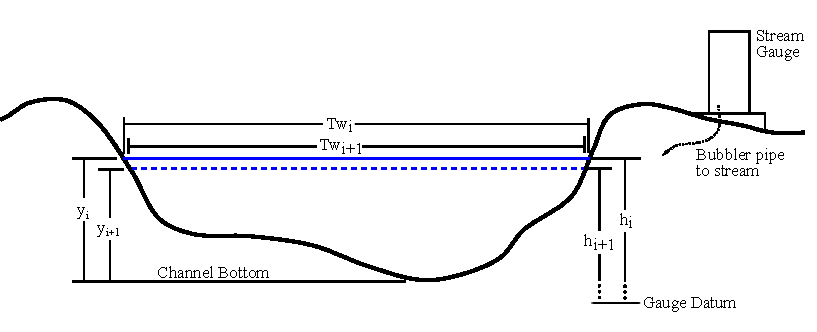
\includegraphics[width=6in]{Figures/LineDiagram/XSection}
	\caption[Average river segment cross-section area change.]{Average river segment cross-section area change.}
	\label{fig:XSArea}
\end{figure}
\begin{figure}
	\centering
		\includegraphics[width=6.5in]{"Figures/LineDiagram/Trapezoid"}
		\caption[River cross-section area change diagram.]{River cross-section area change diagram.}
		\label{fig:XSTrapezoid}
\end{figure}

\begin{align}
	\frac{\Delta A_i}{\Delta t}= & \overline{Tw}\cdot \Delta y \nonumber \\
	\frac{\Delta A_i}{\Delta t} = & \frac{Tw_t + Tw_{t-1}}{2} \cdot \left( y_{t-1} - y_t \right) \label{eq:XSArea}
\end{align}
\begin{tabular}{r p{5.5in}}
	Where: & \\
	$_t$ = & Current time step. \\
	$_{t-1}$ = & Previous time step. \\
	$\displaystyle \frac{\Delta A_i}{\Delta t}$ = & Cross-section area change at river section $ i $ between time steps.\\
	$\overline{Tw}$ = & Average river top width.\\
	$\Delta y$ = & Change in flow depth from the previous time step. \\
	$Tw$ = & River top width. \\
	$y$ = & River flow depth. \\
\end{tabular}\\

Figure \ref{fig:XSArea} shows a simplified river cross section at a stream gauge location.  As previously discussed, stream gauges do not hold the channel bottom as their datum.  They have an arbitrarily fixed datum that does not move unless reset by the gauge owner.  The difference between the stream gauge datum and the channel bottom is corrected using a constant correction factor calculated from the river survey.  The gauge datum does not have a known marker where the elevation could be directly measured.  Instead, the surveyed water surface elevation was recorded at the gauge location on both sides of the channel.  The flow depth value was calculated by finding the difference between the surveyed average water surface elevation and the surveyed channel bottom elevation.  The flow depth was then compared to the stream gauge height reported for the same date and time as when the water surface elevation was surveyed.  The difference between the reported value and the average of the surveyed values was taken as the correction factor for the gauge.  This procedure was repeated for each gauge.

Flow depth values as reported by the USGS and CDWR are measured values with an associated probability range as calculated in equation \ref{eq:uncertainty3}.  The uncertainties are applied as shown in equation \ref{eq:herror1}.  A correction factor ($ C_{i} $) is applied to each reported gauge depth to correct for the difference between the gauge datum and the channel bottom as measured during the channel cross-section survey.  Two separate uncertainties are applied.  $ \varepsilon_{h1} $ is the uncertainty distribution as described by the gauge owner.  This uncertainty is reported by both the USGS and CDWR as being normally distributed with extreme values at \SI{0.01}[$\pm$]{\foot} (\SI{0.003}[$ \pm $]{\meter}) \parencite{USGSPL89}.  The second uncertainty term, $ \varepsilon_{h2} $, is the result of personal observation of the river channel along its entire length.  This term describes the variability in flow depth.  It was observed that the channel depth did not vary greatly along most of its length.  There were particular areas where there were deeper pools, but these areas were noted to be more prone to ponding during low flow.  It is assumed that the average effective flow depth only varies within a normal distribution with limits of \SI{0.076}[$ \pm $]{\meter} (\SI{0.25}[$ \pm $]{\foot}).  There is the possibility that $\varepsilon_{h1}$ could cause the storage change between the time steps to change from a storage gain to a storage loss, or vise versa.  This is acceptable as it is within the measurement limits of the instruments.  Once $h+\varepsilon_{h1}$ has been calculated for the two successive time steps, the relationship between the two time steps is fixed.  If the river segment flow depth rises between time steps after this calculation, then that relationship must continue throughout the rest of the volume change calculation.  To facilitate this, it is assumed that $\varepsilon_{h2}$ does not vary significantly within the study time frame and does not vary within a realization.  The Arkansas River channel is sufficiently stable between consecutive days that this assumption is valid.  A new $\varepsilon_{h2}$ is drawn for each realization and remains constant for all time steps within the study time frame.
\begin{equation}
	y_{i,t}=h_{i,t}+C_{i}+\varepsilon_{h1}+\varepsilon_{h2}
	\label{eq:herror1}
\end{equation}
\begin{tabular}{r p{5.5in}}
	Where: & \\
	$y_{i,t}$  & = Section $ i $ modeled average daily flow depth at time $ t $.\\
	$h_{i,t}$  & = Section $ i $ reported average daily river gauge height at time $ t $.\\
	$ C_{i} $ & = Section $ i $ river gauge height to flow depth correction term.\\
	$\varepsilon_{h1}$ & = Reported river gauge height data uncertainty.\\
	$\varepsilon_{h2}$ & = Estimated flow depth uncertainty.\\
\end{tabular}\\

Since the two uncertainty terms are both normal and additive to flow depth, they were added to produce a new normal distribution with mean equal to the sum of the means of the two distributions and standard deviation equal to the sum of the standard deviations of the two distributions.  This additional step was taken to improve model calculation speed and to reduce the possible error of producing a total flow depth error that would cause a flow depth outside of the accepted range of \SIrange{0.153}{1.53}{\meter} (\SIrange{0.5}{5}{\foot}).  The uncertainty distributions $ \varepsilon_{h1} $ and $ \varepsilon_{h2} $ are not dependent on location, therefore all flow depth calculations draw from the same distribution.  The normal distribution resulting from the addition of the $ \varepsilon_{h1} $ and $ \varepsilon_{h2} $ has a mean of zero and standard deviation of \SI{0.00707}{\meter} (\SI{0.02032}{\foot}) (Equation \ref{eq:herror2}).  
\begin{equation}
	y_{i,t}=h_{i,t}+C_{i}+\mathcal{N} \left( \mu=0m, \sigma=0.00707m \right)
	\label{eq:herror2}
\end{equation}

River top width $ \left( Tw \right)  $ is calculated using equation \ref{eq:Tw1}  \parencite{Buhman2002,Gates1996}. The river channel does not have a fixed cross-section along it's length, therefore, the fitting parameters, $ \beta_1 $ and $ \beta_2 $ are not constant, but are from distributions of  $ \beta_1 $ and $ \beta_2 $.  Equation \ref{eq:Tw1} and the data from each survey cross-section was used to calculate a best fit equation using non-linear least squares regression.  Regression results for each cross-section are presented in Table \ref{tab:alphabetavals}.  There are an insufficient number of cross sections within each river segment to provide a statistically significant sample.  This means that there is insufficient data available to generate independent fitting equations for each river segment.  Therefore, the $ \beta_1 $ and $ \beta_2 $ values from each cross-section were combined to determine the distribution of $ \beta_1 $ and $ \beta_2 $ for the entire river reach.  The combined distributions were tested to determine the best fit parametric distribution using the previously described method.  The best fit distributions for $ \beta_1 $ and $ \beta_2 $ are presented in table \ref{tab:TwFitting}.  $ \beta_1 $ and $ \beta_2 $ values were analyzed for correlation which was found to be insignificant with a Pearson R value of 0.17.  Visual analysis of the data points showed that there was no distinguishable pattern.  Future cross-section surveys will expand the data set and may show that there is a correlation between $ \beta_1 $ and $ \beta_2 $, but the available data does not support that conclusion.  Also presented in Table \ref{tab:TwFitting} is the best fit distribution for the residuals.  These distributions and the distributions for $ \beta_1 $ and $ \beta_2 $ were analyzed to determine the best fit distribution using the methodology described in Section \ref{sec:ErrorAndUncertainty}.

\begin{equation}
	\label{eq:Tw1}
	Tw_{i,t} = \beta_1 y_{i,t} ^{\beta_2} + \varepsilon_{Tw}
\end{equation}
\begin{tabular}{r p{5in}}
	Where: & \\
	$ Tw_{i,t} $ =& River segment $ i $ average daily top width at time step $ t $.\\
	$ y_{i,t} $ =& Calculated segment $ i $ average daily flow depth at time step $ t $ calculated using equation \ref{eq:herror1}.\\
	$ \beta_1 $ and $ \beta_2 $ =& fitting parameter distributions.\\
	$ \varepsilon_{Tw} $=& Calculated average daily flow depth uncertainty.\\
\end{tabular}\\

\begin{table}[htbp]
	\centering
	\caption[Arkansas River segment top width estimating coefficients.]{Arkansas River segment top width estimating coefficients.}
	\label{tab:alphabetavals}
	\begin{tabular}{cccccc}
		\toprule
		Study & River & Cross- & \multicolumn{2}{c}{Fitting Parameter} & Root Mean\\ \cmidrule(l{0.5em}r){4-5}
		Region & Segment & Section & $\beta_1$ & $\beta_2$ & Squared Error\\
		\toprule
		\multirow{21}{*}{USR}& \multirow{4}{*}{A} 		& 1 & 219.1	& 0.5098	& 21.57	\\
		& 						& 2 & 197.5 & 0.01573 &	0.07938 \\
		&						& 3 & 205.2 & 0.7734 & 32.05 \\
		&  						& 4 & 211.5 & 0.008948 & 0.2069 \\ \cmidrule(l{0.5em}r){2-6}
		&  \multirow{3}{*}{B} & 5 & 59.4 & 0.9835 & 0.5002 \\ 
		&						& 6 & 202 & 0.1382 & 12.48 \\ 
		&  						& 7 & 53.99 & 1.197 & 2.412 \\ \cmidrule(l{0.5em}r){2-6}
		& \multirow{5}{*}{C} & 10 & 141 & 0.5465 & 10.92 \\
		&						& 11 & 187.2 & 0.5697 & 7.784 \\
		&						& 12 & 277.9 & 0.01398 & 0.2358	\\ 
		& 						& 13 & 116.5 & 1.536 & 27.5 \\
		&						& 14 & 110 & 0.917 & 1.986 \\ \cmidrule(l{0.5em}r){2-6}
		&\multirow{7}{*}{D}	& 16 & 49.37 & 1.115 & 1.5171 \\ 
		&						& 17 & 57.68 & 1.288 & 1.469 \\
		&						& 18 &116.4 & 0.5197 & 17.42 \\
		&						& 19 & 58.35 & 0.3868 & 6.382 \\ 
		&						& 21 & 141 & 0.07095 & 0.7172 \\
		&						& 22 & 63.82 & 0.6103 & 1.132	\\
		&						& 23 & 109.3 & 0.07456 & 0.4762 \\ \cmidrule(l{0.5em}r){2-6}
		&	E				& 26 & 47.62 & 0.1682 & 0.5901 \\
		\midrule
		\multirow{13}{*}{DSR}& \multirow{7}{*}{F} & 1 & 22.48 & 0.4006 & 0.8139\\
		&						& 2 & 41.61 & 1.390 & 3.953\\
		&						& 3 & 29.82 & 0.2265 & 1.821\\
		& 						& 4 & 21.46 & 0.3801 & 2.541\\
		&						& 5 & 22.78 & 0.8004 & 5.715\\
		&						& 6 & 26.21 & 0.4153 & 1.681\\
		&						& 7 & 41.92 & 1.487 & 3.299\\ \cmidrule(l{0.5em}r){2-6}
		& \multirow{7}[2]{*}{G} & 8 & 23.49 & 1.504 & 2.344\\
		&						& 9 & 33.54 & 1.106 & 3.676\\
		&						& 10& 28.03 & 0.5790 & 2.003\\
		&						& 11& 24.16 & 0.2103 & 1.693\\
		&						& 12& 24.74 & 0.8992 & 2.617\\
		&						& 13& 52.68 & 1.1850 & 5.757\\
		&						& 14& 24.18 & 0.4764 & 0.9259\\
		\bottomrule
	\end{tabular}\\
\end{table}

Non-linear regression models were used only when the specific model form, determined from known physical or geometrical relationships, was non-linear.  R-squared values were not used to determine goodness-of-fit for non-linear regression models since they can have valid R-squared values that are negative or greater than one \parencite{spiess2010} and as such are outside of the boundary for comparing linear models.  Pseudo or modified r-squared calculations are available, yet these computations result in values that are comparable to the r-squared value for linear models, but have slightly different interpretations.  Since non-linear regression models were used only when specific model forms could be predetermined, there was no need to compare different model forms estimating the same result.

Goodness-of-fit for non-linear regressions used in this thesis are purely for informational purposes.  Since all non-linear models were based on known relationships, goodness-of-fit values only serve to show how well the data fits the model.  In order to define non-linear regression model goodness-of-fit, the root mean squared error (RMSE) value was calculated.  The RMSE represents the standard deviation of the differences between the predicted and observed values.  The RMSE is scale dependent as the units are the same as the observed value.  The RMSE is also known as the standard deviation.  This would cause an issue if models for different observed value units and scales were compared against each other.  In this study, non-linear regression models are only used to estimate the cross-sectional width of a river segment and to estimate the selenium concentration at one location.  Since all cross-section analyses use the same measurement units, this allows us to compare the residual errors associated with the various cross sections without needing to consider scale or units.

The results of the top width equation for each cross-section, generated through non-linear regression, was compared to the observed results to visually compare the goodness-of-fit for each cross-section.  Figure \ref{fig:exampleTwVsH} is an example
\begin{figure}[htbp]
	\centering
	\includegraphics[width=6in]{"Figures/Results_USR/Stochastic/Survey Tw vs H-Section 1"}
	\caption[Example Flow Depth vs. River Top Width Relationship.]{Example Flow Depth vs. River Top Width Relationship.  The non-linear best fit line of the form in Equation \ref{eq:Tw1} is red.  The values are the two non-linear regression fitting parameters ($\beta_1$ and $\beta_2$) and the residual standard error for the fitting equation ($\sigma$).  Similar figures for all cross-sections are found in the appendix.}
	\label{fig:exampleTwVsH}
\end{figure}

\begin{table}[htbp]
	\centering
	\caption[River top width fitting parameter distributions.]{River top width fitting parameter distributions.}
	\label{tab:TwFitting}
	\begin{tabular}{ccccc}
		\toprule
		Study                & Fitting   & \multicolumn{3}{c}{Best Fit Distribution} \\ \cmidrule(r{.5em}l){3-5}
		Reach                & Parameter & Dist. Shape      & p1*        & p2*       \\
		\toprule
		\multirow{3}{*}{USR} & $\beta_1$ & logistic         & 16.8       & 7.53      \\
		& $\beta_2$ & log-normal       & -1.27      & 1.57      \\
		& Residual  & logistic         & 1.99       & 0.99      \\
		\midrule
		\multirow{3}{*}{DSR} & $\beta_1$ & logistic         & 28.2       & 4.84      \\
		& $\beta_2$ & log-normal       & -0.43      & 0.65      \\
		& Residual  & log-normal       & 0.87       & 0.57      \\
		\bottomrule
		\multicolumn{5}{l}{{\footnotesize * Distribution fitting parameters.  For logistic, p1=location }}\\
		\multicolumn{5}{l}{\footnotesize{and p2=scale.  For log-normal, p1=mean of the log scale }}\\
		\multicolumn{5}{l}{\footnotesize{and p2=standard dev. of the log scale}}\\
	\end{tabular}\\
\end{table}

Values $\beta_1$ and $\beta_2$ are drawn from probability distributions.  Calculated flow depth and river top width data pairs were used to determine the distributions from which $\beta_1$ and $\beta_2$ in equation \ref{eq:Tw1} were drawn.  These distributions were developed using non-linear, least-squares regression.  Values below \SI{0.15}{\meter} (\SI{0.5}{\foot}) were removed from the regression analysis.  Flow values below this depth are not common and it was determined that these points would not allow for an accurate representation of the flow depth to river top width relationship for the range of known flow depths.  Values above \SI{1.52}{\meter} (\SI{5.0}{\foot}) were also removed from the regression analysis.  Flow depths above this depth are above the banks of the primary river channel and are within the inner flood plain.  Table \ref{tab:alphabetavals} gives the resulting $\beta_1$ and $\beta_2$ values for each surveyed cross-section.  Figure \ref{fig:exampleTwVsH} is an example of the surveyed flow depth and river top width relationships and the derived non-linear relationship for cross-section 1 in river segment A of the USR.  Similar relationship plots for the other surveyed cross-sections are found in the appendix. 

Figure \ref{fig:B1B2} shows the distributions of $\beta_1$ and $\beta_2$ values and the various best-fit distributions in both the USR and DSR.  Logistic, normal, exponential, Weibull, and log-normal distributions were fitted to the data.  Vertical tick marks in the x-axis margin are at the data values.  Kernel density estimations were used as an alternative means to graphically represent the data density.  

\begin{figure}[htbp]
\centering
\begin{subfigure}{0.5\textwidth}
	\centering
	\includegraphics[width=0.9\linewidth]{"Figures/Results_USR/Stochastic/USR B1 Dist"}
	\caption{USR $\beta_1$}
\end{subfigure}%
\begin{subfigure}{0.5\textwidth}
	\centering
	\includegraphics[width=0.9\linewidth]{"Figures/Results_USR/Stochastic/USR B2 Dist"}
	\caption{USR $\beta_2$}
\end{subfigure}
\begin{subfigure}{0.5\textwidth}
	\centering
	\includegraphics[width=0.9\linewidth]{"Figures/Results_DSR/Stochastic/DSR B1 Dist"}
	\caption{DSR $\beta_1$}
\end{subfigure}%
\begin{subfigure}{0.5\textwidth}
	\centering
	\includegraphics[width=0.9\linewidth]{"Figures/Results_DSR/Stochastic/DSR B2 Dist"}
	\caption{DSR $\beta_2$}
\end{subfigure}\\
\caption[$Tw$ Versus $h$ Fitting Parameter $\beta_1$ and $\beta_2$ Distributions.]{$Tw$ Versus $h$ Fitting Parameter $\beta_1$ and $\beta_2$ Distributions.  The black dashed line is a kernel density plot representing a histogram where the bin size approaches zero.  The colored curves are the best fit for the particular distribution type.  Vertical tick marks in the x-axis are at the data values.}
\label{fig:B1B2}
\end{figure}

The resulting river shape parameter distributions are valid for the river reach for which they were calculated.  Each river segment draws values from the shape parameter distributions independently.  Only one pair of shape parameters is drawn for each realization.  It is assumed that the river geometry does not significantly change within the study time frame.  Channel variability is modeled between the realizations.

Residuals from the non-linear regression analyses were combined into a single data set for uncertainty analysis.  Combining this data set was a logical step following the combination of the data that generated the residuals.  Residuals were tested using the same tools and techniques used to test the river shape parameter distributions.  USR and DSR channel shape residuals were found to have a log-normal distribution.  Figure \ref{fig:B1B2 Error} presents the residuals distribution analyses for the USR and DSR.  These figures are of the same type as those used to analyze the river shape parameter distributions, figure \ref{fig:B1B2}.

\begin{figure}[htbp]
\centering
\begin{subfigure}{0.5\textwidth}
	\centering
	\includegraphics[width=0.9\linewidth]{"Figures/Results_USR/Stochastic/USR AB Error Dist"}
	\caption{USR Residuals}
\end{subfigure}%
\begin{subfigure}{0.5\textwidth}
	\centering
	\includegraphics[width=0.9\linewidth]{"Figures/Results_DSR/Stochastic/DSR AB Error Dist"}
	\caption{DSR Residuals}
\end{subfigure}\\
\caption[$Tw$ Versus $H$ Residuals Distribution.]{$Tw$ versus $H$ Residuals Distribution.  The black dashed line is a kernel density plot representing a histogram where the bin size approaches zero.  The colored curves are the best fit for the particular distribution type.  Vertical tick marks in the x-axis are at the data values.}
\label{fig:B1B2 Error}
\end{figure}

Residuals are the collection of the difference between the calculated regression model values and the measured values.  Collectively, the distribution of the residuals describe the uncertainty of the regression model.  In this case, the distribution of residuals describe the top width estimating uncertainty $ \varepsilon_{Tw} $.  Residuals should be tested for heteroskedasticity to determine if the model does not adequately predict the data.  Heteroskedasticity is the condition where the variability of a variable, in this case the residuals, is unequal across the range of the values and is usually indicative of under specification of the model.  There are many tests for heteroskedasticity, but the most powerful is visual analysis of the plot of the residuals against the fitted, or calculated, values.  When a small number of values is used to perform the regression, visual and computational analysis becomes difficult since patterns may appear that don't truly exist or patterns may not appear where they do exist.  When heteroskedasticity was evident during model creation, the model was modified to remove the heteroskedasticity.  Other methods are available to account for heteroskedasticity, but the most strongly recommended is model modification.  Determining the parametric distribution that best fits the regressions is performed using the method described in section \ref{sec:ErrorAndUncertainty}.  Both visual and goodness-of-fit tests were applied to all residual regression analyses.

Results from the individual regression and residuals analyses are plotted with the source data to visually determine if the resulting best fit estimating equation or residuals distribution suitably fit the source data.  An example of one of these figures is Figure \ref{fig:exampleTwVsH} which plots a best fit regression equation alongside the source data.  Figure \ref{fig:B1B2 Error} is representative of how the residual analysis results are visually analyzed.  The best fit of several different distribution shapes are plotted over the histogram and KDE of the residuals or source data.  These types of figures are used throughout the analysis to visually verify that the calculated regression models and best-fit distributions actually fit the data.

Results from deterministic and stochastic models are presented throughout this thesis.  While both model types present results from the same source data, stochastic models, as previously discussed, also include uncertainty in many forms.  Stochastic model results are complex.  They are time-series models where each time step is an independent distribution of the results.  Figure is a very simple representation of a time-series.  The top sub-figure shows a sine curve which represents the deterministic model.  The second sub-figure shows one realization of the stochastic model which is the deterministic model with uncertainty added at each time step.  For this example, the uncertainty is normally distributed within the time step.  The third sub-figure is 500 independent realizations shown on top of each other.  The fourth sub-figure shows the 500 realizations with three calculated lines representing stochastic model summary statistics time-series.

\begin{figure}[htbp]
	\centering
	\includegraphics[width=0.9\linewidth]{"Figures/LineDiagram/TSDescription"}
	\caption[Stochastic model graphical results presentation description.]{Stochastic model graphical results presentation description.  The top sub-figure represents a simple deterministic time-series model.  The second sub-figure represents a single stochastic time-series model.  The third sub-figure represents 500 stochastic time-series.  The fourth sub-figure shows the 500 stochastic time-series with the three stochastic model summary statistics time-series.  The top line is the 97.5th percentile time-series, the middle line is the mean time-series, and the bottom line is the 2.5th percentile time-series.}
	\label{fig:StochExample}
\end{figure}

The middle line is the time-series that represents the mean value calculated for each time-step.  This is the stochastic model mean time-series.  The top and bottom lines are the 97.5th and 2.5th percentile calculated for each time step.  These are the stochastic model 97.5th percentile time-series and stochastic model 2.5th percentile time-series, respectively.  Collectively, these three time-series are called stochastic model summary statistics time-series.  These three time-series show how the results and range of possible results vary with time.  All stochastic time-series graphs present only the three stochastic model summary statistics time-series.  Values outside of these are not plotted so as to improve understanding and readability of the graphical results

Presenting individual values for stochastic model results requires further summary statistics of the calculated stochastic model summary statistics time-series.  Without this further reduction, results would contain large quantities of values which are very difficult to present.  The mean, 97.5th percentile, and 2.5th percentile are calculated for each of the summary statistics time-series to provide more readable results.  The summary statistics for each of the stochastic model summary statistics time-series indicate the most likely value and the range of possible values as presented in the example in Table \ref{tab:ExStochResultsTable}.  In this table, each row of the bottom portion of the table presents one of the stochastic model summary statistic time-series results.  In this example, values '$ g $', '$ h $', and '$ i $' are the summary statistics for the stochastic model mean time-series.

Table \ref{tab:ExStochResultsTable} also includes the deterministic time-series summary statistics values.  These values are the 2.5th percentile, mean, and 97.5th percentile calculated from the deterministic model results and are presented in the upper half of the table.  The deterministic model time-series summary statistics should be approximately the same as the stochastic model mean time-series summary statistics, which are values $ g $,  $ h $, and $ i $ in the lower half of the table.  This statement should be true if the deterministic model is a possible realization of the stochastic model and if the distribution of the combined uncertainties in the stochastic model are approximately normally distributed.

\begin{table}[htbp]
	\centering
	\caption[Example deterministic and stochastic model numerical results.]{Example deterministic and stochastic model numerical results.  The single row on on the deterministic model side presents the summary statistics for the deterministic model (values $ a $, $ b $, and $ c $).  Each row on the stochastic model side presents the results for a specific stochastic model summary time-series.  All values are presented in common units.  The Pearson Correlation value ($ m $) is calculated between the deterministic model time-series and the stochastic model mean time-series values at each time-step in the models.}
	\label{tab:ExStochResultsTable}
	\begin{tabular}{C{1.25in} C{1.4in} C{1.4in} C{1.4in}}
		\toprule
		\multicolumn{4}{l}{\textbf{Deterministic Model Time Series}} \\
		& 2.5th      & \multirow{2}{*}{Mean} & 97.5th   \\
		& Percentile &                       &            Percentile \\ \cmidrule(r{.5em}l){2-4}
		& a			& b			&  c         \\
		\toprule
		\multicolumn{4}{l}{\textbf{Stochastic Model Summary Statistics Time Series}} \\ 
		& 2.5th      & \multirow{2}{*}{Mean} & 97.5th\\
		& Percentile &                       & Percentile \\ \cmidrule(r{.5em}l){2-4}
		97.5th Percentile	& d			& e			& f \\
		Mean						& g			& h			& i \\
		2.5th Percentile	& j			& k			& l \\
		\bottomrule
		\multicolumn{4}{l}{Pearson Correlation = m}
	\end{tabular}\\
\end{table}

One goal of stochastic modeling is to have a deterministic model that resides within the stochastic.  If the deterministic model isn’t a possible realization of the stochastic model, then there are significant stochastic model issues that need to be addressed.  Ideally, the stochastic model mean time-series at each time step should be close to the deterministic model at that same time step.  To determine if this relationship is true, the Pearson correlation between the stochastic model mean time-series and the deterministic model was calculated and is included at the bottom of Table \ref{tab:ExStochResultsTable}.  Calculating the Pearson correlation requires assuming the two compared data sets are continuous and are linearly related.  All input values and results in this thesis are continuous, either from zero to $ +\inf $ or between $ \pm \inf $.

Correlation values only provides a numerical value to describe the relationship between two values or data sets.  It does not imply causality or linearity.  We can infer causality because the deterministic model is a subset of the stochastic model.  In fact, the deterministic model was used to create the stochastic model.  We cannot infer linearity.  Figure \ attempts to answer the linearity issue through visual analysis.  The black dots are the comparison of the stochastic mean time-series and the deterministic model.  The red and blue does are the comparison of the stochastic 97.5th and 2.5th percentile time-series as compared to the deterministic model, respectively.  The solid black line follows the equation y=x.  This is where all of the black dots should lie if the stochastic mean time-series and deterministic models were in perfect agreement.  The dashed line is the quadratic best fit line through the stochastic mean time-series.

\begin{figure}[htbp]
	\centering
	\includegraphics[width=0.9\linewidth]{"Figures/Results_USR/Stochastic/S-D Comparison-M Mass Flow"}
	\caption[Example scatterplot comparing the deterministic model time-series and stochastic model mean time-series results.]{Example scatterplot comparing deterministic model time-series and stochastic model mean time-series results.  The solid line is drawn such that $ y=x $.  The dashed line is the best-fit quadratic equation between the deterministic model time-series and the stochastic model mean time-series and the equation is in the top right. The Pearson Correlation is the top left number.}
	\label{fig:CorrelationExample}
\end{figure}

River segment B in the USR does not have a flow gauge within its boundaries and therefore has no reported flow depths. This segment has an additional irrigation diversion check structure within its boundaries, thereby sub-dividing segment B into two sub-segments, each with its own ungauged flow depth.  Due to segment B being the shortest, composing only 3.9\% of the USR's total length, and the additional variability of the possible flow depth, the average daily flow depth within segment B is taken as the mean of the reported flow depths in segment A and C.  Top width and volume change calculation follows the previously described methodology.

\clearpage
The time-series plots of all four stochastic geometric parameters for each study region river section segment is presented in Figures \ref{fig:GeoTS_US} and \ref{fig:GeoTS_DS} for the USR and DSR, respectively.  The black lines indicate the stochastic model mean time-series.  The blue band indicates the 95\% central inter-percentile range (CIR) of the stochastic values as defined by the stochastic model 2.5th percentile time-series and the stochastic model 97.5th percentile time-series.  The red dashed line in the flow depth portion of the figure indicates the reported flow depth values.  It is plotted under the stochastic model mean time-series line and as such is only visible when either the stochastic model mean time-series value was not calculated due to missing data or when the two values deviate.

\subfiguretop
\begin{landscape}
	\begin{figure}
		\begin{subfigure}{0.7\textwidth}
			\centering
			\includegraphics[width=\tableCustomSize]{"Figures/Results_USR/Stochastic/G TS A"}
			\subcaption*{Segment A}		
			\label{sub:GeoTS_A}
		\end{subfigure}%
		\begin{subfigure}{0.7\textwidth}
			\centering
			\includegraphics[width=\tableCustomSize]{"Figures/Results_USR/Stochastic/G TS B"}
			\subcaption*{Segment B}
			\label{sub:GeoTS_B}
		\end{subfigure}\\
	\caption[USR and DSR stochastic geometric parameter time-series.]{USR and DSR stochastic geometric parameter time-series. The black lines indicate the stochastic model mean time-series.  The blue band indicates the 95\% central inter-percentile range (CIR) of the stochastic values.  The red dashed line in the flow depth portion of the figure indicates the reported flow depth values.}
	\label{fig:GeoTS_US}
	\end{figure}
\end{landscape}

\subfiguremid
\begin{landscape}
	\begin{figure}
		\begin{subfigure}{0.7\textwidth}
			\centering
			\includegraphics[width=\tableCustomSize]{"Figures/Results_USR/Stochastic/G TS C"}
			\subcaption*{Segment C}
			\label{sub:GeoTS_C}	
		\end{subfigure}%
		\begin{subfigure}{0.7\textwidth}
			\centering			
			\includegraphics[width=\tableCustomSize]{"Figures/Results_USR/Stochastic/G TS D"}
			\subcaption*{Segment D}
			\label{sub:GeoTS_D}
		\end{subfigure}\\
		\caption{USR and DSR stochastic geometric parameter time-series.}
	\end{figure}
\end{landscape}

\subfiguremid
\begin{landscape}
	\begin{figure}
		\begin{subfigure}{0.7\textwidth}
			\centering
			\includegraphics[width=\tableCustomSize]{"Figures/Results_USR/Stochastic/G TS E"}
			\subcaption*{Segment E}
			\label{sub:GeoTS_E}	
		\end{subfigure}\\
		\caption{USR and DSR stochastic geometric parameter time-series.}
	\end{figure}
\end{landscape}

\subfiguretop
\begin{landscape}
	\begin{figure}
		\begin{subfigure}{0.7\textwidth}
			\centering
			\includegraphics[width=0.9\textwidth]{"Figures/Results_DSR/Stochastic/G TS F"}
			\subcaption*{Segment F}		
			\label{sub:GeoTS_F}
		\end{subfigure}%
		\begin{subfigure}{0.7\textwidth}
			\centering
			\includegraphics[width=0.9\textwidth]{"Figures/Results_DSR/Stochastic/G TS G"}
			\subcaption*{Segment G}
			\label{sub:GeoTS_G}
		\end{subfigure}
		\caption[DSR stochastic geometric parameter time-series.]{DSR stochastic geometric parameter time-series. The black lines indicate the stochastic model mean time-series.  The blue band indicates the 95\% central inter-percentile range (CIR) of the stochastic values.  The red dashed line in the flow depth portion of the figure indicates the reported flow depth values.}
		\label{fig:GeoTS_DS}
	\end{figure}
\end{landscape}

Figures \ref{fig:GeoTS_US} and \ref{fig:GeoTS_DS} were analyzed to verify that direct correlations existed between the flow depth and the calculated geometric parameters.  Top width and surface area should increase and decrease in proportion with the increase and decrease in flow depth.  Volume changes are based on two flow depth values and do not have a direct correlation to the flow depth displayed in the figure.  All of the river sections show the correct correlations between flow depth and the calculated river geometric parameters.

Tables \ref{tab:SegmentSurfaceArea_USR} and \ref{tab:SegmentSurfaceArea_DSR} present the river segment average daily surface area deterministic model time-series and stochastic model summary statistic time-series results for the USR and DSR, respectively.  Summary results for river segment average daily flow depth and river segment average daily top width are not included as they are not direct precursors to the final model results.  The surface area is directly used for precipitation and evaporation calculations.

\subtabletop
\begin{table}[htbp]
	\centering
	\caption[USR river segment surface area deterministic and stochastic model numerical results.]{USR river segment surface area deterministic and stochastic model numerical results.  Values are in hectares (\si{\hectare}) with values in parentheses in acres (\si{\acre}).}
	\label{tab:SegmentSurfaceArea_USR}
	\begin{subtable}{\textwidth}
		\centering
		\subcaption*{USR river segment A}
		\input{"Tables/tableAreaA.txt"}
	\end{subtable}\\
	\tablevspace
	\begin{subtable}{\textwidth}
		\centering
		\subcaption*{USR river segment B}
		\input{"Tables/tableAreaB.txt"}
	\end{subtable}\\
\end{table}

\subtablemid
\begin{table}[htbp]
	\centering
	\caption{USR river segment surface area deterministic and stochastic model numerical results.}
	\begin{subtable}{\textwidth}
		\centering
		\subcaption*{USR river segment C}
		\input{"Tables/tableAreaC.txt"}
	\end{subtable}\\
	\tablevspace
	\begin{subtable}{\textwidth}
		\centering
		\subcaption*{USR river segment D}
		\input{"Tables/tableAreaD.txt"}
	\end{subtable}\\
\end{table}

\subtablemid
\begin{table}[htbp]
	\centering
	\caption{USR river segment surface area deterministic and stochastic model numerical results.}
	\begin{subtable}{\textwidth}
		\centering
		\subcaption*{USR river segment E}
		\input{"Tables/tableAreaE.txt"}
	\end{subtable}\\
\end{table}

\subtabletop
\begin{table}[htbp]
	\centering
	\caption[DSR river segment surface area deterministic and stochastic model numerical results.]{DSR river segment surface area deterministic and stochastic model numerical results.  Values are in hectares (\si{\hectare}) with values in parentheses in acres (\si{\acre}).}
	\label{tab:SegmentSurfaceArea_DSR}
	\begin{subtable}{\textwidth}
		\centering
		\subcaption*{DSR river segment F}
%		\input{"Tables/tableAreaF.txt"}
	\end{subtable}\\
	\tablevspace
	\begin{subtable}{\textwidth}
		\centering
		\subcaption*{DSR river segment G}
%		\input{"Tables/tableAreaG.txt"}
	\end{subtable}\\
\end{table}

Every one of these tables shows that the stochastic model tends to underestimate the river segment water surface area by approximately 38\% in the USR and XX\% in the DSR.  The correlation values indicate that the deterministic model time-series and stochastic model mean time-series are highly correlated.  The corresponding correlation scatter-plots show that the relationships are linear.  This is due to the way the river section average daily top width was estimated for the deterministic models.  Since $ \beta_1 $ and $ \beta_2 $ are drawn from distributions and the deterministic model requires that none of the input values are variable, the most likely values from the respective distributions were chosen as the fixed values.  The $ \beta $ values from both study reaches are not normal, therefore the most likely value is not the mean and the values are not evenly distributed on either side of the likely value.  The skewness of the $ \beta $ values is represented in the stochastic model.  Calibrating the deterministic models to find the $ \beta $ values that approximate the stochastic model defeats the purpose of the deterministic model, which is to estimate the most likely values.  Sensitivity analysis which is discussed later, will show whether or not the river section average daily surface area values are significant enough to warrant the effort required to calibrate them to the stochastic model.

Tables \ref{tab:SegmentVolumeChange_USR} and \ref{tab:SegmentVolumeChange_DSR} present the river segment average daily surface area deterministic model time-series and stochastic model summary statistic time-series results for the USR and DSR, respectively.  Summary results for river segment average daily flow depth and river segment average daily top width are not included as they are not direct precursors to the final model results.  The surface area is directly used for precipitation and evaporation calculations.
\\
\subtabletop
\begin{table}[htbp]
	\centering
	\caption[USR river segment volume change deterministic and stochastic model numerical results.]{USR river segment volume change deterministic and stochastic model numerical results.  Values are in hectare-meters (\si{\hectare\meter}) and the values in parentheses are in acres (\si{\acre}).}
	\label{tab:SegmentVolumeChange_USR}
	\begin{subtable}{\textwidth}
		\centering
		\subcaption*{USR river segment A}
		\input{"Tables/tableVolumeA.txt"}
	\end{subtable}\\
	\tablevspace
	\begin{subtable}{\textwidth}
		\centering
		\subcaption*{USR river segment B}
		\input{"Tables/tableVolumeB.txt"}
	\end{subtable}\\
\end{table}	
\subtablemid
\begin{table}[htbp]
	\centering
	\caption{USR river segment volume change deterministic and stochastic model numerical results.}
	\begin{subtable}{\textwidth}
		\centering
		\subcaption*{USR river segment C}
		\input{"Tables/tableVolumeC.txt"}
	\end{subtable}\\
	\tablevspace
	\begin{subtable}{\textwidth}
		\centering
		\subcaption*{USR river segment D}
		\input{"Tables/tableVolumeD.txt"}
	\end{subtable}\\
\end{table}
\subtablemid
\begin{table}[htbp]
	\centering
	\caption{USR river segment volume change deterministic and stochastic model numerical results.}
	\begin{subtable}{\textwidth}
		\centering
		\subcaption*{USR river segment E}
		\input{"Tables/tableVolumeE.txt"}
	\end{subtable}\\
	\tablevspace
\end{table}

\subtabletop
\begin{table}[htbp]
	\centering
	\caption[DSR river segment volume change deterministic and stochastic model numerical results.]{DSR river segment volume change deterministic and stochastic model numerical results.  Values are in hectare-meters (\si{\hectare\meter}) and the values in parentheses are in acres (\si{\acre}).}
	\label{tab:SegmentVolumeChange_DSR}
	\begin{subtable}{\textwidth}
		\centering
		\subcaption*{DSR river segment F}
		\input{"Tables/G volF.txt"}
	\end{subtable}\\
	\tablevspace	
	\begin{subtable}{\textwidth}
		\centering
		\subcaption*{DSR river segment G}
		\input{"Tables/G volG.txt"}
	\end{subtable}\\
\end{table}	

The mean of the deterministic model time-series and the mean of the stochastic model mean time-series calculated average daily river segment water volume change are much closer to each other as reported in Tables \ref{tab:SegmentVolumeChange_USR} and \ref{tab:SegmentVolumeChange_DSR}.  The stochastic model mean time-series underestimates the deterministic model time-series values by approximately 47\%.  The difference between the two models in terms of water volume is quite small, less than \SI{1}{\hectare\meter}.  The Pearson correlation values and their associated scatter-plots indicate that the results are strongly linearly related.  The effects of uncertainty on river segment average river daily water volume change is much smaller than the effect on surface area.  As with the surface area results, the significant portion of the difference between the deterministic model time-series and the stochastic model mean time-series is due to the estimation of the most likely values of $ \beta_1 $ and $ \beta_2 $ used in the deterministic models.  At this point, adjusting or calibrating these values such that the results of the deterministic and stochastic models are more closely aligned seems unnecessary.

Figure \ref{fig:USRWaterStore} and \ref{fig:DSRWaterStore} presents the river reach average daily river water storage change deterministic model time-series for the USR and DSR, respectively, as calculated using Equation \ref{eq:storage1}.  The left-hand figure is the deterministic model time-series.  The right-hand figure is the stochastic model results with the black line representing the calculated stochastic model mean time-series and the blue band representing the space between the stochastic model 97.5th percentile time-series and the stochastic model 2.5th percentile time-series.  The minimum and maximum range of values is not presented in this figure.

\begin{figure}[htbp]
\centering
	\begin{subfigure}{0.5\textwidth}
		\centering
		\includegraphics[width=0.9\linewidth]{"Figures/Results_USR/Deterministic/Balance Water - storage"}
		\subcaption*{Deterministic Model.}
		\label{sub:USRWaterStoreD}
	\end{subfigure}%
	\begin{subfigure}{0.5\textwidth}
		\centering
		\includegraphics[width=0.9\linewidth]{"Figures/Results_USR/Stochastic/Balance Water - storage"}
		\subcaption*{Stochastic Model.}
		\label{sub:USRWaterStoreS}
	\end{subfigure}\\
	\caption[USR Arkansas River water storage change contribution to the water model.]{USR Arkansas River water storage change contribution to the water model.}
	\label{fig:USRWaterStore}
\end{figure}

\begin{figure}[htbp]
	\centering
	\begin{subfigure}{0.5\textwidth}
		\centering
		\includegraphics[width=0.9\linewidth]{"Figures/Results_DSR/Deterministic/Balance Water - storage"}
		\subcaption*{Deterministic Model.}
	\end{subfigure}%
	\begin{subfigure}{0.5\textwidth}
		\centering
		\includegraphics[width=0.9\linewidth]{"Figures/Results_DSR/Stochastic/Balance Water - storage"}
		\subcaption*{Stochastic Model.}
	\end{subfigure}\\
	\caption[DSR Arkansas River water storage change contribution to the water model.]{DSR Arkansas River water storage change contribution to the water model.}
	\label{fig:DSRWaterStore}
\end{figure}

Tables xx presents the deterministic model time-series summary statistics and the summary statistics for each of the stochastic model summary statistics time-series for the river reach average daily water storage change in the USR and DSR.

\begin{table}[htbp]
	\centering
	\caption[USR river reach average daily stored water volume change.]{USR river reach average daily stored water volume change.  Values in hectare-meters (\si{\hectare\meter\per\kilo\meter}) and values in parentheses in acre-feet (\si{\acre\foot\per\mile})}
	\label{tab:waterStorage-US}
	\subcaption*{ $\displaystyle\frac{\Delta S_{DSR}}{\Delta t} $ }
	\input{"Tables/USRVolume.txt"}
\end{table}
	\tablevspace
\begin{table}[htbp]
	\centering
	\caption[DSR river reach average daily stored water volume change.]{DSR river reach average daily stored water volume change.  Values in hectare-meters (\si{\hectare\meter\per\kilo\meter}) and values in parentheses in acre-feet (\si{\acre\foot\per\mile})}
	\label{tab:waterStorage-DS}
	\subcaption*{ $\displaystyle\frac{\Delta S_{USR}}{\Delta t} $ }
	\input{"Tables/DSRVolume.txt"}
\end{table}

The figures show that there is a definite seasonal variation in the storage component.  Stored water changes are smallest during the cold months and are increasingly larger during the growing season.  This pattern is caused by irrigation practices in the Lower Arkansas River Basin (LARV).  Stored irrigation water is released from reservoirs upstream of the LARV during the irrigation season as demands require.  During the winter, there is very little to no irrigation occurring.  This, combined with the low precipitation and no additional flow from snow-pack runoff, allow flows in the Arkansas River to reach base flow level when the river is at a natural equilibrium.

This pattern is not as pronounced in the DSR.  This is most likely due to required flow rates being maintained at the Colorado-Kansas border.  With the constant required flow, John Martin Reservoir releases only enough water to meet the required flow rate.  This creates a flow regime that is nearly constant through most of the DSR. 

Deviations are noted during peak irrigation season.  These additional volume changes are most likely due to irrigation flows returning to the Arkansas River from fields irrigated from canal systems that procure and store water upstream of John Martin Reservoir.  The Fort Lyon Storage Canal and Fort Lyon Canal are two examples of canal systems that perform this function.  Water removed from the USR, stored, and added to the DSR is not included in this study.

The distribution of all realizations within each time step was analyzed to determine a distribution type.  This analysis was performed to determine if the assumption that the deterministic model results were representative of the stochastic model.   Testing was performed by comparing K-S statistics for the best fit normal and logistic distributions.  Log-normal, logistic, exponential, gamma, and Weibull distributions were considered, but were not included in this analysis since they do not support the full range of possible values, $ (-\infty, +\infty) $.  The non-included distributions could have been scaled and shifted, but they are still limited in the range of possible values.  In the USR and the DSR, all of the river water volume storage change stochastic model time steps are best fit by a logistic distribution.
  
The mean of the percent difference between the deterministic model time-series and stochastic model mean time-series is very low.  This indicates that the deterministic model is representative of the stochastic model expected value.  The high percent differences at the 2.5th and 97.5th percentile indicate that there is still a large range of uncertainty contained within the stochastic model that the deterministic model cannot replicate.  The deterministic model can be used to determine how changes can affect a reach over a span of time, but using it to estimate values for specific time steps is unwise as the differences noted at individual time steps is too large to account for.
\clearpage{}

\section{Gauged Stream Flows and Diverted Canal Flows}
\label{sec:StreamFlows}

Equation \ref{eq:water1} contains the portion contained in equation \ref{eq:flow1} that describes the sum of all accountable surface water flows entering and leaving a defined reach.  These flows include only the gauged river main stem flows, tributary stream flows, and diverted canal flows.  Most flows are reported as average daily flow rate.  These flow rates, which are measured every 15 minutes, are calculated from the respective gauge's measured instantaneous stage height using stage-discharge tables.  The only exception is with the average daily flow rate reported for the La Junta waste water treatment plant where the average daily flow is converted from the total daily discharge, reported in million gallons per day (mgd).

\begin{equation}
\label{eq:flow1}
\sum Q_{Total} = \left( Q_{out,DS} + \sum Q_{out} - Q_{in,US} - \sum Q_{in} \right) 
\end{equation}
\begin{tabular}{r p{5.5in}}
	Where: & \\
	$ Q_{Total} = $ & sum of average daily flow rates in the study region.\\
	$ Q_{in} = $ & flow entering the study reach from a tributary.\\
	$ Q_{out} = $ & flow leaving the study reach to an irrigation canal.\\
	$ Q_{in,US} = $ & flow entering the study reach in the main stem of the river at the upstream end of the reach.\\
	$ Q_{out,DS} = $ & flow leaving the study reach in the main stem of the river at the downstream end of the reach.\\
\end{tabular}\\

Equation \ref{eq:flow1} is expanded as follows to contain all of the measured flows entering or leaving the main stem of the Arkansas River within the USR boundaries.  The subscript for each flow in equation \ref{eq:USRFlow} is the CDWR symbol for a particular gauge site.  See the map in Figure \ref{USRSample} for the gauge locations in the USR.  The flows in this equation are ordered by location along the main stem of the river, from upstream to downstream.
\begin{align}
	\label{eq:USRFlow}
	\sum Q_{Total,USR} = &~Q_{ARKCATCO} - Q_{HOLCANCO} - Q_{RFDMANCO} - Q_{FLSCANCO} \\
	\nonumber & + Q_{RFDRETCO} + Q_{TIMSWICO} - Q_{FLYCANCO} + Q_{CANSWKCO} \\ 
	\nonumber & + Q_{LAJWWTP} - Q_{CONDITCO} + Q_{HRC194CO} - Q_{ARKLASCO}
\end{align}
Where each subscript is defined as the flow through the gauge described in Table \ref{tab:USRFlow}.  In this table, each of the flow variables in equation \ref{eq:USRFlow}, designated by its CDWR gauge name, is grouped by the type of flow using the variables used in equation \ref{eq:flow1}.

\begin{table}[htbp]
	\centering
	\caption[Description of USR stream flow variables.]{Description of USR stream flow variables.  The CDWR gauge name is the USR model variable sub-script.  The variable group is the category to which the flow belongs.}
	\label{tab:USRFlow}
	\begin{tabular}{c C{1in} p{3.5in}}
		\toprule
		CDWR Gauge & Variable & \multirow{2}{*}{Description}\\
		Name				& Group & \\
		\toprule
		$ ARKCATCO $ & $ Q_{in,US} $ & Arkansas River below the Catlin Canal diversion.\\ 
		$ HOLCANCO $ & $ Q_{out} $ & Holbrook Canal \\
		$ RFDMANCO $ & $ Q_{out} $ & Rocky Ford Canal\\
		$ FLSCANCO $ & $ Q_{out} $ & Fort Lyon Storage Canal\\
		$ RFDRETCO $ & $ Q_{in} $ & Rocky Ford Return Ditch\\
		$ TIMSWICO $ & $ Q_{in} $ & Timpas Creek\\
		$ FLYCANCO $ & $ Q_{out} $ & Fort Lyon Canal\\
		$ CANSWKCO $ & $ Q_{in} $ & Crooked Arroyo\\
		$ LAJWWTP $ & $ Q_{in} $ & Discharge from the La Junta WWTP\\
		$ CONDITCO $ & $ Q_{out} $ & Consolidated Ditch (Jones Ditch)\\
		$ HRC194CO $ & $ Q_{in} $ & Horse Creek at Colorado Highway 194\\
		$ ARKLASCO $ & $ Q_{out,DS} $ & Arkansas River in Las Animas, Colorado\\
		\bottomrule
	\end{tabular}\\
\end{table}

For the DSR, equation \ref{eq:flow1} is expanded as follows to contain all of the measured flows entering or leaving the main stem of the Arkansas River within its boundaries.  The subscript for each flow in equation \ref{eq:DSRFlow} is the CDWR symbol for a particular gauge site.  See the map in Figure \ref{DSRSample} for the gauge locations in the DSR.  The flows in this equation are ordered by location along the main stem of the river, from upstream to downstream.
\begin{align}
	\label{eq:DSRFlow}
	\sum Q_{Total,DSR} = &~Q_{ARKLAMCO} + Q_{BIGLAMCO} - Q_{BUFDITCO} + Q_{WILDHOCO} \\
	\nonumber & - Q_{FRODITKS} - Q_{ARKCOOKS}
\end{align}
Where each subscript is defined as the flow through the gauge described in Table \ref{tab:DSRFlow}.  In this table, each of the flow variables in equation \ref{eq:DSRFlow}, designated by its CDWR gauge name, is grouped by the type of flow using the variables used in equation \ref{eq:water1}.

\begin{table}[htbp]
	\centering
	\caption[Description of DSR stream flow variables.]{Description of DSR stream flow variables.  The CDWR gauge name is the DSR model variable sub-script.  The variable group is the category to which the flow belongs.}
	\label{tab:DSRFlow}
	\begin{tabular}{c C{1in} p{3.5in}}
		\toprule
		CDWR Gauge & Variable & \multirow{2}{*}{Description}\\
		Name				& Group & \\
		\toprule
		$ ARKLAMCO $ & $ Q_{in,US} $ & Arkansas River in Lamar, Colorado\\ 
		$ BIGLAMCO $ & $ Q_{in} $ & Big Sandy Creek \\
		$ BUFDITCO $ & $ Q_{out} $ & Buffalo Ditch\\
		$ WILDHOCO $ & $ Q_{in} $ & Wild Horse Creek\\
		$ FRODITKS $ & $ Q_{out} $ & Frontier Ditch\\
		$ ARKCOOKS $ & $ Q_{out,DS} $ & Arkansas River in Coolidge, Kansas\\
		\bottomrule
	\end{tabular}\\
\end{table}

Equations \ref{eq:USRFlow} and \ref{eq:DSRFlow} constitute the surface water flow portion of \ref{eq:flow1} for the USR and DSR deterministic models, respectively.  As with the other portions of the water balance models, converting these to be used in the stochastic models requires the addition of uncertainty terms.
\begin{equation}
	\label{eq:flow1error}
	Q_{stochastic} = Q_{reported} + \varepsilon_{Q_{reported}}
\end{equation}
\begin{tabular}{r p{5.5in}}
	Where:\\
	$ Q_{stochastic} $& = flow rate through a gauge used in the stochastic model.\\
	$ Q_{reported}  $ & = flow rate through a gauge as reported by the USGS or CDWR.\\
	$ \varepsilon_{Q_{reported}} $ &= reported gauge uncertainty for a specific stream gauge.\\
\end{tabular}\\

Using Equation \ref{eq:flow1error} with very low flow values may result in negative flow rates.  Therefore, $Q_{stochastic}$ was calculated using a truncated normal distribution where the minimum allowed value was \SI{0}{\cubic\meter\per\second} (\SI{0}{\cubic\foot\per\second}), the maximum allowed value was 1.25 times the maximum reported value for the specific stream gauge, and the mean value was the reported flow rate value.  Truncation was performed using an algorithm within the statistical software that used re-sampling and replacement.  Other methods were available, but they were deemed to be less reliable.

Stream flow data is provided as described in Section \ref{sec:data collected by other sources}  The USGS provides three specific uncertainty distributions for average daily stream flow data which are described in every annual water data report \parencite{USGS2006NWIS, USGS2007NWIS, USGS2008NWIS, USGS2009NWIS, USGS2010NWIS, USGS2011NWIS, USGS2012NWIS}.  The USGS calls these uncertainty distributions "ratings of accuracy".  These ratings are "excellent", "good", and "fair".  The "excellent" rating indicates that "the daily discharges are within 5 percent of the true value".  The distributions expand to 10\% and 15\% for "good" and "fair" ratings, respectively.  There is a fourth rating used on some average daily stream flow data gathered in the LARV; "poor".  This rating is not specific as it states that the values are more than 15\% of the true value.  For this thesis, we have refined the "poor" rating definition such that 95 percent of the values are within 20 percent of the true value.  These ratings are as shown in Table \ref{tab:USGSError} which was extracted from a USGS annual water data report.

\begin{table}[htbp]
	\caption[USGS Measured Field Parameter Accuracy Rating Table.]{USGS Measured Field Parameter Accuracy Rating Table.  This table was taken from the USGS annual water data report. }
	\label{tab:USGSError}
	\includegraphics[width=6in]{"Figures/USGS_error_table"}
\end{table}

Figures \ref{fig:GaugeFlow_US} and \ref{fig:GaugeFlow_DS} present the stochastic and deterministic model results for each of the stream flow variables used in USR and DSR models, respectively.  Each pair of figures presents the deterministic model results on the left and the stochastic model results on the right.  The deterministic model figures show the flow rates as reported by the CDWR and USGS.  The stochastic model figures present the stochastic model mean time-series and the band bounded by the stochastic model 2.5th percentile time-series and the stochastic model 97.5th percentile time-series.  These figures present results from each of the stream gauge in CDWR stream gauge name alphabetical order.

\subfiguretop
\begin{landscape}
	\begin{figure}
		\centering
		$ Q_{ARKCATCO} $
		\begin{subfigure}{0.7\textwidth}
			\centering
			\includegraphics[width=\tableCustomSize]{"Figures/Results_USR/Deterministic/Q U163"}
			\subcaption*{Deterministic}		
		\end{subfigure}%
		\begin{subfigure}{0.7\textwidth}
			\centering
			\includegraphics[width=\tableCustomSize]{"Figures/Results_USR/Stochastic/Q U163"}
			\subcaption*{Stochastic}
		\end{subfigure}\\
		\caption[USR deterministic and stochastic model time-series average daily flow rate.]{USR deterministic and stochastic model time-series average daily flow rate.  The deterministic model time-series presents the data reported by the CDWR and USGS gauges.  In the stochastic model time-series, the black lines indicate the stochastic model mean time-series.  The blue band indicates the 95\% central inter-percentile range (CIR) of the stochastic values.  Results are presented in CDWR stream gauge name alphabetical order.}
		\label{fig:GaugeFlow_US}
	\end{figure}
\end{landscape}
\subfiguremid
\begin{landscape}
	\begin{figure}
		\centering
		$ Q_{ARKLASCO} $
		\begin{subfigure}{0.7\textwidth}
			\centering
			\includegraphics[width=\tableCustomSize]{"Figures/Results_USR/Deterministic/Q U201"}
			\subcaption*{Deterministic}		
		\end{subfigure}%
		\begin{subfigure}{0.7\textwidth}
			\centering
			\includegraphics[width=\tableCustomSize]{"Figures/Results_USR/Stochastic/Q U201"}
			\subcaption*{Stochastic}
		\end{subfigure}\\
		\caption{USR deterministic and stochastic model time-series average daily flow rate.}
	\end{figure}
\end{landscape}
\subfiguremid
\begin{landscape}
	\begin{figure}
		\centering
		$ Q_{CANSWKCO} $
		\begin{subfigure}{0.7\textwidth}
			\centering
			\includegraphics[width=\tableCustomSize]{"Figures/Results_USR/Deterministic/Q CAN"}
			\subcaption*{Deterministic}		
		\end{subfigure}%
		\begin{subfigure}{0.7\textwidth}
			\centering
			\includegraphics[width=\tableCustomSize]{"Figures/Results_USR/Stochastic/Q CAN"}
			\subcaption*{Stochastic}
		\end{subfigure}\\
		\caption{USR deterministic and stochastic model time-series average daily flow rate.}
	\end{figure}
\end{landscape}
\subfiguremid
\begin{landscape}
	\begin{figure}
		\centering
		$ Q_{CONDITCO} $
		\begin{subfigure}{0.7\textwidth}
			\centering
			\includegraphics[width=\tableCustomSize]{"Figures/Results_USR/Deterministic/Q CON"}
			\subcaption*{Deterministic}		
		\end{subfigure}%
		\begin{subfigure}{0.7\textwidth}
			\centering
			\includegraphics[width=\tableCustomSize]{"Figures/Results_USR/Stochastic/Q CON"}
			\subcaption*{Stochastic}
		\end{subfigure}\\
		\caption{USR deterministic and stochastic model time-series average daily flow rate.}
	\end{figure}
\end{landscape}
\subfiguremid
\begin{landscape}
	\begin{figure}
		\centering
		$ Q_{FLSCANCO} $
		\begin{subfigure}{0.7\textwidth}
			\centering
			\includegraphics[width=\tableCustomSize]{"Figures/Results_USR/Deterministic/Q FLS"}
			\subcaption*{Deterministic}		
		\end{subfigure}%
		\begin{subfigure}{0.7\textwidth}
			\centering
			\includegraphics[width=\tableCustomSize]{"Figures/Results_USR/Stochastic/Q FLS"}
			\subcaption*{Stochastic}
		\end{subfigure}\\
		\caption{USR deterministic and stochastic model time-series average daily flow rate.}
	\end{figure}
\end{landscape}
\subfiguremid
\begin{landscape}
	\begin{figure}
		\centering
		$ Q_{FLYCANCO} $
		\begin{subfigure}{0.7\textwidth}
			\centering
			\includegraphics[width=\tableCustomSize]{"Figures/Results_USR/Deterministic/Q FLY"}
			\subcaption*{Deterministic}		
		\end{subfigure}%
		\begin{subfigure}{0.7\textwidth}
			\centering
			\includegraphics[width=\tableCustomSize]{"Figures/Results_USR/Stochastic/Q FLY"}
			\subcaption*{Stochastic}
		\end{subfigure}\\
		\caption{USR deterministic and stochastic model time-series average daily flow rate.}
	\end{figure}
\end{landscape}
\subfiguremid
\begin{landscape}
	\begin{figure}
		\centering
		$ Q_{HOLCANCO} $
		\begin{subfigure}{0.7\textwidth}
			\centering
			\includegraphics[width=\tableCustomSize]{"Figures/Results_USR/Deterministic/Q HOL"}
			\subcaption*{Deterministic}		
		\end{subfigure}%
		\begin{subfigure}{0.7\textwidth}
			\centering
			\includegraphics[width=\tableCustomSize]{"Figures/Results_USR/Stochastic/Q HOL"}
			\subcaption*{Stochastic}
		\end{subfigure}\\
		\caption{USR deterministic and stochastic model time-series average daily flow rate.}
	\end{figure}
\end{landscape}
\subfiguremid
\begin{landscape}
	\begin{figure}
		\centering
		$ Q_{HRC194CO} $
		\begin{subfigure}{0.7\textwidth}
			\centering
			\includegraphics[width=\tableCustomSize]{"Figures/Results_USR/Deterministic/Q HRC"}
			\subcaption*{Deterministic}		
		\end{subfigure}%
		\begin{subfigure}{0.7\textwidth}
			\centering
			\includegraphics[width=\tableCustomSize]{"Figures/Results_USR/Stochastic/Q HRC"}
			\subcaption*{Stochastic}
		\end{subfigure}\\
		\caption{USR deterministic and stochastic model time-series average daily flow rate.}
	\end{figure}
\end{landscape}
\subfiguremid
\begin{landscape}
	\begin{figure}
		\centering
		$ Q_{LAJWWTP} $
		\begin{subfigure}{0.7\textwidth}
			\centering
			\includegraphics[width=\tableCustomSize]{"Figures/Results_USR/Deterministic/Q WTP"}
			\subcaption*{Deterministic}		
		\end{subfigure}%
		\begin{subfigure}{0.7\textwidth}
			\centering
			\includegraphics[width=\tableCustomSize]{"Figures/Results_USR/Stochastic/Q WTP"}
			\subcaption*{Stochastic}
		\end{subfigure}\\
		\caption{USR deterministic and stochastic model time-series average daily flow rate.}
	\end{figure}
\end{landscape}
\subfiguremid
\begin{landscape}
	\begin{figure}
		\centering
		$ Q_{RFDMANCO} $
		\begin{subfigure}{0.7\textwidth}
			\centering
			\includegraphics[width=\tableCustomSize]{"Figures/Results_USR/Deterministic/Q RFD"}
			\subcaption*{Deterministic}		
		\end{subfigure}%
		\begin{subfigure}{0.7\textwidth}
			\centering
			\includegraphics[width=\tableCustomSize]{"Figures/Results_USR/Stochastic/Q RFD"}
			\subcaption*{Stochastic}
		\end{subfigure}\\
		\caption{USR deterministic and stochastic model time-series average daily flow rate.}
	\end{figure}
\end{landscape}
\subfiguremid
\begin{landscape}
	\begin{figure}
		\centering
		$ Q_{RFDRETCO} $
		\begin{subfigure}{0.7\textwidth}
			\centering
			\includegraphics[width=\tableCustomSize]{"Figures/Results_USR/Deterministic/Q RFR"}
			\subcaption*{Deterministic}		
		\end{subfigure}%
		\begin{subfigure}{0.7\textwidth}
			\centering
			\includegraphics[width=\tableCustomSize]{"Figures/Results_USR/Stochastic/Q RFR"}
			\subcaption*{Stochastic}
		\end{subfigure}\\
		\caption{USR deterministic and stochastic model time-series average daily flow rate.}
	\end{figure}
\end{landscape}
\subfiguremid
\begin{landscape}
	\begin{figure}
		\centering
		$ Q_{TIMSWICO} $
		\begin{subfigure}{0.7\textwidth}
			\centering
			\includegraphics[width=\tableCustomSize]{"Figures/Results_USR/Deterministic/Q TIM"}
			\subcaption*{Deterministic}		
		\end{subfigure}%
		\begin{subfigure}{0.7\textwidth}
			\centering
			\includegraphics[width=\tableCustomSize]{"Figures/Results_USR/Stochastic/Q TIM"}
			\subcaption*{Stochastic}
		\end{subfigure}\\
		\caption{USR deterministic and stochastic model time-series average daily flow rate.}
	\end{figure}
\end{landscape}
\subfiguremid
\begin{landscape}
	\begin{figure}
		\centering
		$ Q_{LaJuntaWWTP} $
		\begin{subfigure}{0.7\textwidth}
			\centering
			\includegraphics[width=\tableCustomSize]{"Figures/Results_USR/Deterministic/Q WTP"}
			\subcaption*{Deterministic}		
		\end{subfigure}%
		\begin{subfigure}{0.7\textwidth}
			\centering
			\includegraphics[width=\tableCustomSize]{"Figures/Results_USR/Stochastic/Q WTP"}
			\subcaption*{Stochastic}
		\end{subfigure}\\
		\caption{USR deterministic and stochastic model time-series average daily flow rate.}
	\end{figure}
\end{landscape}



\subfiguretop
\begin{landscape}
	\begin{figure}
		\centering
		$ Q_{ARKLASCO} $
		\begin{subfigure}{0.7\textwidth}
			\centering
			\includegraphics[width=\tableCustomSize]{"Figures/Results_DSR/Deterministic/Q in"}
			\subcaption*{Deterministic}		
		\end{subfigure}%
		\begin{subfigure}{0.7\textwidth}
			\centering
			\includegraphics[width=\tableCustomSize]{"Figures/Results_DSR/Stochastic/Q in"}
			\subcaption*{Stochastic}
		\end{subfigure}\\
		\caption[DSR deterministic and stochastic model time-series average daily flow rate.]{DSR deterministic and stochastic model time-series average daily flow rate.  The deterministic model time-series presents the data reported by the CDWR and USGS gauges.  In the stochastic model time-series, the black lines indicate the stochastic model mean time-series.  The blue band indicates the 95\% central inter-percentile range (CIR) of the stochastic values.  Results are presented in CDWR stream gauge name alphabetical order.}
		\label{fig:GaugeFlow_DS}
	\end{figure}
\end{landscape}
\subfiguremid
\begin{landscape}
	\begin{figure}
		\centering
		$ Q_{ARKCOOKS} $
		\begin{subfigure}{0.7\textwidth}
			\centering
			\includegraphics[width=\tableCustomSize]{"Figures/Results_DSR/Deterministic/Q out"}
			\subcaption*{Deterministic}		
		\end{subfigure}%
		\begin{subfigure}{0.7\textwidth}
			\centering
			\includegraphics[width=\tableCustomSize]{"Figures/Results_DSR/Stochastic/Q out"}
			\subcaption*{Stochastic}
		\end{subfigure}\\
		\caption{DSR deterministic and stochastic model time-series average daily flow rate.}
	\end{figure}
\end{landscape}
\subfiguremid
\begin{landscape}
	\begin{figure}
		\centering
		$ Q_{BIGLAMCO} $
		\begin{subfigure}{0.7\textwidth}
			\centering
			\includegraphics[width=\tableCustomSize]{"Figures/Results_DSR/Deterministic/Q BIG"}
			\subcaption*{Deterministic}		
		\end{subfigure}%
		\begin{subfigure}{0.7\textwidth}
			\centering
			\includegraphics[width=\tableCustomSize]{"Figures/Results_DSR/Stochastic/Q BIG"}
			\subcaption*{Stochastic}
		\end{subfigure}\\
		\caption{DSR deterministic and stochastic model time-series average daily flow rate.}
	\end{figure}
\end{landscape}
\subfiguremid
\begin{landscape}
	\begin{figure}
		\centering
		$ Q_{BUFDITCO} $
		\begin{subfigure}{0.7\textwidth}
			\centering
			\includegraphics[width=\tableCustomSize]{"Figures/Results_DSR/Deterministic/Q BUF"}
			\subcaption*{Deterministic}		
		\end{subfigure}%
		\begin{subfigure}{0.7\textwidth}
			\centering
			\includegraphics[width=\tableCustomSize]{"Figures/Results_DSR/Stochastic/Q BUF"}
			\subcaption*{Stochastic}
		\end{subfigure}\\
		\caption{DSR deterministic and stochastic model time-series average daily flow rate.}
	\end{figure}
\end{landscape}
\subfiguremid
\begin{landscape}
	\begin{figure}
		\centering
		$ Q_{FRODITKS} $
		\begin{subfigure}{0.7\textwidth}
			\centering
			\includegraphics[width=\tableCustomSize]{"Figures/Results_DSR/Deterministic/Q FRO"}
			\subcaption*{Deterministic}		
		\end{subfigure}%
		\begin{subfigure}{0.7\textwidth}
			\centering
			\includegraphics[width=\tableCustomSize]{"Figures/Results_DSR/Stochastic/Q FRO"}
			\subcaption*{Stochastic}
		\end{subfigure}\\
		\caption{DSR deterministic and stochastic model time-series average daily flow rate.}
	\end{figure}
\end{landscape}
\subfiguremid
\begin{landscape}
	\begin{figure}
		\centering
		$ Q_{WILDHOCO} $
		\begin{subfigure}{0.7\textwidth}
			\centering
			\includegraphics[width=\tableCustomSize]{"Figures/Results_DSR/Deterministic/Q WIL"}
			\subcaption*{Deterministic}		
		\end{subfigure}%
		\begin{subfigure}{0.7\textwidth}
			\centering
			\includegraphics[width=\tableCustomSize]{"Figures/Results_DSR/Stochastic/Q WIL"}
			\subcaption*{Stochastic}
		\end{subfigure}\\
		\caption{DSR deterministic and stochastic model time-series average daily flow rate.}
	\end{figure}
\end{landscape}

Both figures \ref{fig:GaugeFlow_US} and \ref{fig:GaugeFlow_DS} show that the stochastic model mean time-series of each of the calculated stochastic model flow rates does not deviate significantly from the deterministic model time-series.  Tables \ref{tab:GaugeFlow_US} and \ref{tab:GaugeFlow_DS} present the numeric results associated with each of the figures.  These tables show that the deterministic model time-series and stochastic mean time-series are essentially identical.  The 2.5th percentile, mean, and 97.5th percentile of the two models are identical or nearly identical for all flow rates.  The Pearson Correlation values for the two models are 1 or very nearly 1 for all cases.  These results show that for the average daily flow rate, the deterministic model is representative of the stochastic model

\subtabletop
\begin{table}[htbp]
	\centering
	\caption[USR deterministic and stochastic model time-series average daily flow rate numeric results.]{USR deterministic and stochastic model time-series average daily flow rate numeric results.  Results are presented in CDWR stream gauge name alphabetical order.}
	\label{tab:GaugeFlow_US}
	\begin{subtable}{\textwidth}
		\centering
		\subcaption*{$ Q_{ARKCATCO} $}
		\input{"Tables/USR_qIN.txt"}
	\end{subtable}\\
	\tablevspace
	\begin{subtable}{\textwidth}
		\centering
		\subcaption*{$ Q_{ARKLASCO} $}
		\input{"Tables/USR_qOUT.txt"}
	\end{subtable}\\
\end{table}
\subtablemid
\begin{table}[htbp]
	\centering
	\caption{USR deterministic and stochastic model time-series average daily flow rate numeric results.}
	\begin{subtable}{\textwidth}
		\centering
		\subcaption*{$ Q_{CANSWKCO} $}
		\input{"Tables/USR_qCAN.txt"}
	\end{subtable}\\
	\tablevspace
	\begin{subtable}{\textwidth}
		\centering
		\subcaption*{$ Q_{CONDITCO} $}
		\input{"Tables/USR_qCON.txt"}
	\end{subtable}\\
\end{table}	
\subtablemid
\begin{table}[htbp]
	\centering
	\caption{USR deterministic and stochastic model time-series average daily flow rate numeric results.}
	\begin{subtable}{\textwidth}
		\centering
		\subcaption*{$ Q_{FLSCANCO} $}
		\input{"Tables/USR_qFLS.txt"}
	\end{subtable}\\
	\tablevspace
	\begin{subtable}{\textwidth}
		\centering
		\subcaption*{$ Q_{FLYCANCO} $}
		\input{"Tables/USR_qFLY.txt"}
	\end{subtable}\\
\end{table}
\subtablemid
\begin{table}[htbp]
	\centering
	\caption{USR deterministic and stochastic model time-series average daily flow rate numeric results.}
	\begin{subtable}{\textwidth}
		\centering
		\subcaption*{$ Q_{HOLCANCO} $}
		\input{"Tables/USR_qHOL.txt"}
	\end{subtable}\\
	\tablevspace
	\begin{subtable}{\textwidth}
		\centering
		\subcaption*{$ Q_{HRC194CO} $}
		\input{"Tables/USR_qHRC.txt"}
	\end{subtable}\\
\end{table}
\subtablemid
\begin{table}[htbp]
	\centering
	\caption{USR deterministic and stochastic model time-series average daily flow rate numeric results.}
	\begin{subtable}{\textwidth}
		\centering
		\subcaption*{$ Q_{RFDMANCO} $}
		\input{"Tables/USR_qRFD.txt"}
	\end{subtable}\\
	\tablevspace
	\begin{subtable}{\textwidth}
		\centering
		\subcaption*{$ Q_{RFDRETCO} $}
		\input{"Tables/USR_qRFR.txt"}
	\end{subtable}\\
\end{table}
\subtablemid
\begin{table}[htbp]
	\centering
	\caption{USR deterministic and stochastic model time-series average daily flow rate numeric results.}
	\begin{subtable}{\textwidth}
		\centering
		\subcaption*{$ Q_{TIMSWICO} $}
		\input{"Tables/USR_qTIM.txt"}
	\end{subtable}\\
	\tablevspace
	\begin{subtable}{\textwidth}
		\centering
		\subcaption*{$ Q_{LaJunta WWTP} $}
		\input{"Tables/USR_qWTP.txt"}
	\end{subtable}\\
\end{table}

\subtabletop
\begin{table}[htbp]
	\centering
	\caption[DSR deterministic and stochastic model time-series average daily flow rate numeric results.]{DSR deterministic and stochastic model time-series average daily flow rate numeric results.  Results are presented in CDWR stream gauge name alphabetical order.}
	\label{tab:GaugeFlow_DS}
	\begin{subtable}{\textwidth}
		\centering
		\subcaption*{$ Q_{ARKLAMCO} $}
		\input{"Tables/DSR_qIN.txt"}
	\end{subtable}\\
	\tablevspace
	\begin{subtable}{\textwidth}
		\centering
		\subcaption*{$ Q_{ARKCOOKS} $}
		\input{"Tables/DSR_qOUT.txt"}
	\end{subtable}\\
\end{table}
\subtablemid
\begin{table}[htbp]
	\centering
	\caption{DSR deterministic and stochastic model time-series average daily flow rate numeric results.}
	\begin{subtable}{\textwidth}
		\centering
		\subcaption*{$ Q_{BIGLAMCO} $}
		\input{"Tables/DSR_qBIG.txt"}
	\end{subtable}\\
	\tablevspace
	\begin{subtable}{\textwidth}
		\centering
		\subcaption*{$ Q_{BUFDITCO} $}
		\input{"Tables/DSR_qBUF.txt"}
	\end{subtable}\\
\end{table}
\subtablemid
\begin{table}[htbp]
	\centering
	\caption{DSR deterministic and stochastic model time-series average daily flow rate numeric results.}
	\begin{subtable}{\textwidth}
		\centering
		\subcaption*{$ Q_{WILDHOCO} $}
		\input{"Tables/DSR_qWIL.txt"}
	\end{subtable}\\
	\tablevspace
	\begin{subtable}{\textwidth}
		\centering
		\subcaption*{$ Q_{FRODITKS} $}
		\input{"Tables/DSR_qFRO.txt"}
	\end{subtable}\\
\end{table}
\clearpage
Average daily flow rates are not grouped and calculated by river segment.  Figures \ref{fig:reachFlow_US} and \ref{fig:reachFlow_DS} and Tables \ref{tab:reachFlow_US} and \ref{tab:reachFlow_DS}present the results of the flow portion of the water balance model calculated as shown in Equations \ref{eq:USRFlow} and \ref{eq:DSRFlow} for the USR and DSR, respectively.  Figures \ref{fig:reachFlow_US} and \ref{fig:reachFlow_DS} show the sum of the deterministic model flow rates in the left figure.  The right figure shows the sum of the stochastic model flow rates.  As with the other stochastic model figures, the black line depicts the stochastic model mean time-series and the blue region depicts the range of values between the stochastic model 97.5th percentile time-series and the stochastic model 2.5th percentile time-series.  Values outside of this range are not included in the figures.  The figures and associated tables are presented in units of \si{\cubic\meter\per\second\per\kilo\meter} (\si{\cfs\per\mile}).  Standardizing the results to present values in units of storage per unit length allows for comparisons to be made between the two study reaches and between water balance model components.  Positive values indicate that the respective reach gains water due to gauged surface water flows.

\subfiguretop
\begin{landscape}
	\begin{figure}
		\centering
		$ \displaystyle \sum Q_{Total,USR} $
		\begin{subfigure}{0.7\textwidth}
			\centering
			\includegraphics[width=\tableCustomSize]{"Figures/Results_USR/Deterministic/Balance Water - flow"}
			\subcaption*{Deterministic}		
		\end{subfigure}%
		\begin{subfigure}{0.7\textwidth}
			\centering
			\includegraphics[width=\tableCustomSize]{"Figures/Results_USR/Stochastic/Balance Water - flow"}
			\subcaption*{Stochastic}
		\end{subfigure}\\
		\caption[USR deterministic and stochastic model time-series reach flow rates.]{USR deterministic and stochastic model time-series reach flow rates.  In the stochastic model time-series, the black lines indicate the stochastic model mean time-series.  The blue band indicates the 95\% central inter-percentile range (CIR) of the stochastic values.}
		\label{fig:reachFlow_US}
	\end{figure}
\end{landscape}
\subfiguretop
\begin{landscape}
	\begin{figure}
		\centering
		$ \displaystyle \sum Q_{Total,DSR} $
		\begin{subfigure}{0.7\textwidth}
			\centering
			\includegraphics[width=\tableCustomSize]{"Figures/Results_DSR/Deterministic/Balance Water - flow"}
			\subcaption*{Deterministic}		
		\end{subfigure}%
		\begin{subfigure}{0.7\textwidth}
			\centering
			\includegraphics[width=\tableCustomSize]{"Figures/Results_DSR/Stochastic/Balance Water - flow"}
			\subcaption*{Stochastic}
		\end{subfigure}\\
		\caption[DSR deterministic and stochastic model time-series reach flow rates.]{DSR deterministic and stochastic model time-series reach flow rates.  In the stochastic model time-series, the black lines indicate the stochastic model mean time-series.  The blue band indicates the 95\% central inter-percentile range (CIR) of the stochastic values.}
		\label{fig:reachFlow_DS}
	\end{figure}
\end{landscape}

\subtabletop
\begin{table}[htbp]
	\centering
	\caption[USR deterministic and stochastic model time-series reach total average daily flow rate numeric results.]{USR deterministic and stochastic model reach total time-series average daily flow rate numeric results.  Flow rates are presented in units of \si{\cubic\meter\per\second\per\kilo\meter} (\si{\cfs\per\mile}).}
	\label{tab:reachFlow_US}
	\subcaption*{$\displaystyle \sum Q_{Total,USR} $}
	\input{"Tables/USRFlow.txt"}
\end{table}
\tablevspace
\begin{table}[htbp]
	\centering
	\caption[DSR deterministic and stochastic model time-series reach total average daily flow rate numeric results.]{DSR deterministic and stochastic model reach total time-series average daily flow rate numeric results.  Flow rates are presented in units of \si{\cubic\meter\per\second\per\kilo\meter} (\si{\cfs\per\mile}).}
	\label{tab:reachFlow_DS}
	\subcaption*{$\displaystyle \sum Q_{Total,DSR} $}
	\input{"Tables/DSRFlow.txt"}
\end{table}

The individual gauged flow rate figures and the reach calculated sum of gauged flow rate figures show that there is a definite seasonal variation in the flow rates.  This is as expected since the LARV water supply is highly dependent on irrigation waters provided by reservoir releases.  The values in the reach tables show that the stochastic model mean time-series closely follows the deterministic model time-series.  The summary statistics of the two models and the Pearson Correlation between the two models are nearly identical.  This shows that the gauge flow portion of the deterministic water balance model is a very good representation of the stochastic model.  

Each of the time-steps of this portion of the USR stochastic model were analyzed to determine the best fit distribution using K-S analysis.  Of the tested possible distribution shapes, all of the time steps had logistic distributions.  Visual analysis of the relationship between the date and the best fit distribution did not yield any significance.  Similarly, visual analysis of the relationship between the resultant flow rate and the best fit distribution did not yield any significance. 

The DSR stochastic model underwent the same analysis.  Of the tested possible distribution shapes, 98.3\% of the time-steps were best fit by logistic distributions.  The remaining 1.7\% were best fit by normal distributions.  Visual analysis of the comparison between the time-step date and the best fit distribution showed that all of the normally distributed time-steps are at the beginning of the study time frame.   Visual analysis of the comparison between the region volume change and the best fit distribution revealed that the few time-steps that were normally distributed, were characterized as low magnitude storage loss time-steps.

The reach flow summary time-series figures (\ref{fig:GaugeFlow_US} and\ref{fig:GaugeFlow_US}) show that there is a definite seasonal variation in the flow component.  The surface water flow balance changes from being a losing system to a gaining system during the irrigation season.  This pattern is caused by irrigation practices in the Lower Arkansas River Basin (LARV).  Excess irrigation water applied to fields runs off into tributaries which feed into the Arkansas River

The figures also show that the river is discharging more water than it receives.  In the USR, this matches the general observed trend where the upstream end of the reaches receives more water than the downstream ends discharges.  This does not match the observed trend in the DSR where the flows at the upstream end appear to be less than or equal to the flows at the downstream end.  In the DSR, this mismatch between the observed phenomenon and the measured values indicates that another process is a significant contributor to the flow regime.  Since the two reaches are in the same environment, it is reasonable to assume that the same phenomenon is present in the USR.  It is suspected that groundwater from the riparian aquifer is the unaccounted for source in both the USR and DSR.

The reach flow summary time-series summary statistics tables (\ref{tab:GaugeFlow_US} and \ref{tab:GaugeFlow_DS}) show that the deterministic model is very similar to the stochastic model mean time-series.  The similarity between the table values and the high Pearson Correlation lead to the determination that the deterministic model is representative of the stochastic model expected value.  


\section{Atmospheric Contributions to the Water Balance Models}
Atmospheric effects on the river within the USR and DSR is limited to evaporation and precipitation as shown in Equation \ref{eq:atm1}.
\begin{align}
	\label{eq:atm1}
	\sum Q_{Atm}&=P-E\\
		\label{eq:atm2}
		& = P \cdot \sum A_i - E \cdot \sum A_i
\end{align}
\begin{tabular}{r p{5in}}
	Where:& \\
	$ \displaystyle \sum Q_{Atm} $ = & Total effects of precipitation and evaporation on the flow balance model, expressed as a the change in volume per time-step.\\ 
	$ P $ = & Reported total daily precipitation.\\
	$ E $ = & Calculated total daily evaporation.\\
	$ \displaystyle \sum A_i  $ = & Sum of the river reach segment surface areas as previously calculated. \\
\end{tabular}\\

This equation is the form used earlier in this thesis.  While it is the traditional form, it assumes that $ P $ and $ E $ are expressed as flow.  This is not the usual case.  Both $ P $ and $ E $ are usually expressed in units of depth per time-step.  Multiplying these values by the affected surface area results in a volume change per time-step (Equation \ref{eq:atm3}).  This may be more appropriately labeled as the change in storage due to atmospheric effects per time-step $ \displaystyle \left( \frac{\Delta S_{Atm}}{\Delta t} \right) $.  This is a philosophical argument, and the decision was made to refer to the atmospheric effects as shown in Equation \ref{eq:atm3}.

Evaporation from natural water bodies is not directly measured. At best, evaporation pans when used appropriately, are used to estimate evaporation from nearby natural bodies.  Yet, even these require the use of a calibrated coefficient before the data is relatively reliable.  For this thesis, evaporation data was gathered and treated as discussed in Section \ref{sec:data collected by other sources}.  This data was provided as the total daily reference evapo-transpiration $ \left( ET_{ref} \right) $ as calculated using the ASCE EWRI tall crop reference equation.  This equation is identical to the Food and Agriculture Organization of the United Nations (FAO) Penman-Montieth equation \parencite{walter2000asce,FAO56} and is calculated as follows with variables in appropriate SI units:
\begin{equation}
\label{eq:ET}
	ET_{ref}=\frac{0.408\Delta(R_n-G)+\gamma \displaystyle \frac{C_n}{T+273}u_2(e_s-e_a)}{\Delta+\gamma(1+0.34u_2)}
\end{equation}
\begin{tabular}{r p{5.5in}}
Where: &\\
$ET_{ref}$ =&standardized reference crop evapotranspiration for short or tall surfaces. \\
$R_n$ =&calculated net radiation at the crop surface. \\
$G$ =&soil heat flux density at the soil surface. \\
$T$ =&mean daily air temperature at 1.5 to 2.5 meter height. \\
$u_2$ =&mean daily wind speed at 2 meter height. \\
$e_s$ =&saturation vapor pressure at 1.5 to 2.5 meter height, calculated as the
average of saturation vapor pressure at minimum and maximum air temperature. \\
$e_a$ =&mean actual vapor pressure at 1.5 to 2.5 meter height . \\
$\Delta$ =&slope of the saturation vapor pressure-temperature curve. \\
$\gamma$ =&psychrometric constant . \\
$c_n$ =&numerator constant that changes with reference type. \\
$C_d$ =&denominator constant that changes with reference type. \\
\end{tabular}\\

This equation is quite complex and it was determined that independent calculation would not be of any benefit.  This equation also does not provide the necessary value of $ E $, but of  $ ET_{ref} $, which is a reference value that describes the total of the evaporation $ (E) $ and transpiration $ (T) $ from a reference crop under ideal conditions.  Converting $ ET_{ref} $ into $ E $ requires the use of conversion equations found in FAO56.  The open water coefficient, $K_w$, is used to perform this conversion.  The FAO has an extensive set of crop coefficients including coefficients for open water for use on the FAO Penman-Montieth (FAO PM) equation.  
\begin{equation}
\label{eq:ETcoef}
E=K_w \cdot ET_{ref}
\end{equation}
\begin{tabular}{r p{5.5in}}
Where:&\\
$E$ = & Evaporation\\
$K_w$ = & Open water coefficient\\
$ET_{ref}$ = & ASCE EWRI Standardized Reference Evapotranspiration Equation, tall crop equation.\\
\end{tabular}\\

The FAO developed the $K_w$ values for the short reference crop $ET_ref$ equation.  Use of crop coefficients developed for the short crop reference equation with the tall crop (alfalfa) reference equation is prohibited  \parencite{FAO56, Allen2011}.  Equation \ref{eq:ET Kconversion} is used to convert crop coefficients for use between the two ET reference equation results \parencite{FAO56}.
\begin{equation}
\label{eq:ET Kconversion}
	K_{w}=K_\mathsf{ratio} \cdot K_{wt}
\end{equation}
\begin{tabular}{r p{5.5in}}
Where:&\\
$K_\mathsf{ratio}$ =& conversion factor, calculated using equation \ref{eq:ET Kratio}\\
$K_{ws}$ =& short crop based crop coefficient, \\
$K_{wt}$ =& tall crop based crop coefficient.\\
\end{tabular}\\

\begin{equation}
\label{eq:ET Kratio}
	K_\mathsf{ratio}=K_{ws}+[0.04(u_2-2)-0.004(RH_{min}-45)] \left(\frac{h}{3} \right)^{0.3}
\end{equation}
\begin{tabular}{r l}
Where:&\\
$h$ =& 0.5 meters as the standard height for the tall crop reference.
\end{tabular}\\

There is no reported error associated with the use of equations \ref{eq:ET Kconversion} or \ref{eq:ET Kratio}.  However, there are known uncertainties in the reported minimum daily relative humidity and average daily wind speed.  Both relative humidity and wind speed uncertainties are based on equipment uncertainty and do not include any other sources of uncertainty.  Precipitation, minimum daily relative humidity, and wind speed data error provided through the CoAgMet system was based solely on instrument accuracy and was reported as $\pm1\%$ for precipitation, $\pm2\%$ for minimum daily relative humidity, and $\pm0.5~m \cdot s^{-1}$ for wind speed.  These values are based on the typical instruments installed at the various locations.  Sensors vary somewhat between observation sites due to equipment replacement.  Colorado Climate Network personnel have stated that replacement equipment either meets or exceeds the equipment on a typical observation site.  The uncertainty distributions for these three weather measurements was assumed to be normal with 95\% of the values within the reported range of the true value.

A preliminary analysis of this method resulted in $K_\mathsf{ratio}$ values shows a mean value of 1.097 and a standard deviation of 0.049.  The $K_\mathsf{ratio}$ values are best fit by a logistic distribution with a location parameter of 1.099 and a scale parameter of 0.0266.  Using the FAO $K_{ws}$ value of 1.05 results in an average $K_{wt}$ value of 0.95 using equation \ref{eq:ET Kconversion}.  Jensen suggests using $K_{ws}=1.10$ based on data from Alamosa, Colorado, which results in an average $K_{wt}$ value of 1.00.

This seems to suggest that unlike the short crop $ET_{ref}$ equation, the tall crop $ET_{ref}$ over estimates evaporation from a shallow water body.  This seems plausible as surface area is a significant factor in determining evaporation.  A mature, 0.5 meter tall alfalfa crop has a large leaf area which could plausibly exceed the equivalent surface area of open water.  

Atmospheric data obtained from CoAgMet does not have publicly defined uncertainty distributions.  At the time this thesis, a study headed by Dr.\ Jos\'{e} L.\ Ch\'{a}vez at Colorado State University was underway to evaluate the ASCE EWRI standardized alfalfa ET reference Penman-Montieth equation with relation to lysimetric data in Colorado.  Preliminary findings provided by Dr. Ch\'{a}vez indicate an average daily reference ET mean bias error of $-0.47~mm \cdot day^{-1}$ with a variability of $\pm 0.98~mm \cdot day^{-1}$ when compared to lysimetric data.  The bias error indicates that the reported $ET_{ref}$ underestimates the actual ET.  The measurement variability is reported as the root mean square error (RMSE), or standard deviation, of the measurement.

Figures \ref{fig:reachEvap_US} and \ref{fig:reachEvap_DS} show the deterministic and stochastic model time-series of evaporation in \si{\milli\meter} for the USR and DSR respectively.  Tables \ref{tab:reachEvap_US} and \ref{tab:reachEvap_DS} present the associated summary statistics for the deterministic time-series and the summary statistics for the three calculated stochastic model time-series.

\subfiguretop
\begin{landscape}
	\begin{figure}
		\centering
		$ \displaystyle \overline{E}_{USR} $
		\begin{subfigure}{0.7\textwidth}
			\centering
			\includegraphics[width=\tableCustomSize]{"Figures/Results_USR/Deterministic/A Evap"}
			\subcaption*{Deterministic}		
		\end{subfigure}%
		\begin{subfigure}{0.7\textwidth}
			\centering
			\includegraphics[width=\tableCustomSize]{"Figures/Results_USR/Stochastic/A Evap"}
			\subcaption*{Stochastic}
		\end{subfigure}\\
		\caption[USR deterministic and stochastic model time-series total estimated evaporation.]{USR deterministic and stochastic model time-series total estimated evaporation.  In the stochastic model time-series, the black lines indicate the stochastic model mean time-series.  The blue band indicates the 95\% central inter-percentile range (CIR) of the stochastic values.}
		\label{fig:reachEvap_US}
	\end{figure}
\end{landscape}
\subfiguretop
\begin{landscape}
	\begin{figure}
		\centering
		$ \displaystyle \overline{E}_{DSR} $
		\begin{subfigure}{0.7\textwidth}
			\centering
			\includegraphics[width=\tableCustomSize]{"Figures/Results_DSR/Deterministic/A Evap"}
			\subcaption*{Deterministic}		
		\end{subfigure}%
		\begin{subfigure}{0.7\textwidth}
			\centering
			\includegraphics[width=\tableCustomSize]{"Figures/Results_DSR/Stochastic/A Evap"}
			\subcaption*{Stochastic}
		\end{subfigure}\\
		\caption[DSR deterministic and stochastic model time-series total estimated evaporation.]{DSR deterministic and stochastic model time-series total estimated evaporation.  In the stochastic model time-series, the black lines indicate the stochastic model mean time-series.  The blue band indicates the 95\% central inter-percentile range (CIR) of the stochastic values.}
		\label{fig:reachEvap_DS}
	\end{figure}
\end{landscape}

\subtabletop
\begin{table}[htbp]
	\centering
	\caption[USR deterministic and stochastic model time-series total estimated evaporation numeric results.]{USR deterministic and stochastic model time-series total estimated evaporation numeric results.  Total daily evaporation rates are presented in units of \si{\milli\meter} (\si{\inch}).}
	\label{tab:reachEvap_US}
	\subcaption*{$\displaystyle \overline{E}_{USR} $}
	\input{"Tables/USR Evap.txt"}
\end{table}
\tablevspace
\begin{table}[htbp]
	\centering
	\caption[DSR deterministic and stochastic model time-series total estimated evaporation numeric results.]{DSR deterministic and stochastic model time-series total estimated evaporation numeric results.  Total daily evaporation rates are presented in units of \si{\milli\meter} (\si{\inch}).}
	\label{tab:reachEvap_DS}
	\subcaption*{$\displaystyle \overline{E}_{DSR} $}
	\input{"Tables/DSR Evap.txt"}
\end{table}

Precipitation in the study regions is not well defined.  An assumption was made that precipitation was not uniformly distributed over either study region.  Reports from field technicians, conversation with local residents, and personal experience indicate that most storms during the summer were isolated and relatively small.  It was not known by the end of this study whether weather radar data was available or could be used to more accurately estimate rainfall onto the Arkansas River water surface.  It was assumed that, at best, 50\% of any rain event would add water directly to the river.  The reported precipitation depth value was modified by a factor of 0.5 to reflect the estimated average storm coverage for the region.  The atmospheric contribution to the models is taken as the sum of the modified precipitation and evaporation values with the assumption that all precipitation values are positive and all evaporation values are negative as shown in equation \ref{eq:atm4}.

\begin{equation}
\sum Q_{Atm} = 0.5 \cdot \overline{P} \cdot \sum A_{i} - K_{wt} \cdot \overline{ET_{Ref}} \cdot \sum A_{i}
\label{eq:atm4}
\end{equation}
Where\\
\begin{tabular}{r p{5.5in}}
	$Q_{Atm} =$&Total water volume gained (+) or lost (-) due to atmospheric contributions for a study region river section. Values calculated and presented as average daily flow rates.\\
	$\overline{P} =$&Regional average precipitation taken as the mean of the reporting regional rain gauges.\\
	$K_{wt} =$& Open water coefficient for the tall $ET_{Ref}$ equation.\\
	$\overline{ET_{ref}} =$&Regional average $ET_{Ref}$ taken as the mean of the reporting regional reference ET gauges.\\
	$\sum A_{i}=$&Sum of calculated reach surface areas within a study region river section. \\
\end{tabular}\\

Figures \ref{fig:reachPrecip_US} and \ref{fig:reachPrecip_DS} show the deterministic and stochastic model time-series of precipitation depth in \si{\milli\meter} for the USR and DSR respectively.  Tables \ref{tab:reachPrecip_US} and \ref{tab:reachPrecip_DS} present the associated summary statistics for the deterministic time-series and the summary statistics for the three calculated stochastic model time-series.

\subfiguretop
\begin{landscape}
	\begin{figure}
		\centering
		$ \displaystyle \overline{P}_{USR} $
		\begin{subfigure}{0.7\textwidth}
			\centering
			\includegraphics[width=\tableCustomSize]{"Figures/Results_USR/Deterministic/A Precip"}
			\subcaption*{Deterministic}		
		\end{subfigure}%
		\begin{subfigure}{0.7\textwidth}
			\centering
			\includegraphics[width=\tableCustomSize]{"Figures/Results_USR/Stochastic/A Precip"}
			\subcaption*{Stochastic}
		\end{subfigure}\\
		\caption[USR deterministic and stochastic model time-series total estimated precipitation.]{USR deterministic and stochastic model time-series total estimated precipitation.  In the stochastic model time-series, the black lines indicate the stochastic model mean time-series.  The blue band indicates the 95\% central inter-percentile range (CIR) of the stochastic values.}
		\label{fig:reachPrecip_US}
	\end{figure}
\end{landscape}
\subfiguretop
\begin{landscape}
	\begin{figure}
		\centering
		$ \displaystyle \overline{P}_{DSR} $
		\begin{subfigure}{0.7\textwidth}
			\centering
			\includegraphics[width=\tableCustomSize]{"Figures/Results_DSR/Deterministic/A Precip"}
			\subcaption*{Deterministic}		
		\end{subfigure}%
		\begin{subfigure}{0.7\textwidth}
			\centering
			\includegraphics[width=\tableCustomSize]{"Figures/Results_DSR/Stochastic/A Precip"}
			\subcaption*{Stochastic}
		\end{subfigure}\\
		\caption[DSR deterministic and stochastic model time-series total estimated precipitation.]{DSR deterministic and stochastic model time-series total estimated precipitation.  In the stochastic model time-series, the black lines indicate the stochastic model mean time-series.  The blue band indicates the 95\% central inter-percentile range (CIR) of the stochastic values.}
		\label{fig:reachPrecip_DS}
	\end{figure}
\end{landscape}

\subtabletop
\begin{table}[htbp]
	\centering
	\caption[USR deterministic and stochastic model time-series total estimated precipitation numeric results.]{USR deterministic and stochastic model time-series total estimated precipitation numeric results.  Total daily precipitation  rates are presented in units of \si{\milli\meter} (\si{\inch}).}
	\label{tab:reachPrecip_US}
	\subcaption*{$\displaystyle \overline{P}_{USR} $}
	\input{"Tables/USR Precip.txt"}
\end{table}
\tablevspace
\begin{table}[htbp]
	\centering
	\caption[DSR deterministic and stochastic model time-series total estimated precipitation numeric results.]{DSR deterministic and stochastic model time-series total estimated precipitation numeric results.    Total daily precipitation  rates are presented in units of \si{\milli\meter} (\si{\inch}).}
	\label{tab:reachPrecip_DS}
	\subcaption*{$\displaystyle \overline{P}_{DSR} $}
	\input{"Tables/DSR Precip.txt"}
\end{table}

The blue band in both $ P $ figures, which depicts the 95th CIR, is very small and is nearly indistinguishable from the stochastic mean time-series values.  This indicates that the $ P $ measurement uncertainty is very small.  A cyclical pattern is easily noted when observing the $ E $ and $ P $ values in both the USR and DSR.  We note that both daily total $ E $ and $ P $ are higher during warmer months and lower during cold months.  The cyclical nature of the daily $ E $ agrees with common knowledge where evaporation rates are higher as average temperatures rise.  The cyclical nature of the daily precipitation agrees with climate analyses by the National Weather Service which state that most of the precipitation in the LARV occurs with thunder storms during the warmer months.

It is interesting to note that during the 4 year time span calculated in this study annual average evaporation rates appear to increase and annual average precipitation rates appear to decrease.  The time frame of this study is too short to conclude anything about the long term climate of the region.  This observation may be useful when observing other results produced in this study.

The difference between the deterministic model time-series and the stochastic model mean time-series summary statistics as noted in the tables is very low for the $ E $ and $ P $ values in both the USR and DSR.  This, and the very high Pearson Correlation values, indicate that the deterministic model accurately represents the expected value of the stochastic model.

The value $ \displaystyle \sum A_i  $, as used in equation \ref{eq:atm4}, is the reach average daily surface area as previously calculated for the deterministic and stochastic models.  These surface area values are calculated based on the calculated river top width values used to calculate the river volume change.  No changes were made to the previous river geometry calculations before being used to estimate total precipitation gains to and evaporative losses from the river.

Total reach atmospheric contribution gains and losses in units of \si{\cubic\meter\per\second\per\kilo\meter} are presented in Figures \ref{fig:reachAtm_US} and \ref{fig:reachAtm_DS} for the USR and DSR, respectively  These figures show the volume of water gained or lost for each day scaled by the length of the respective reach for comparative purposes.  For the USR and DSR, respectively, tables \ref{tab:reachAtm_US} and \ref{tab:reachAtm_DS} present the deterministic model time-series summary statistics and the summary statistics for the stochastic model mean time-series, the stochastic model 97.5th percentile time-series, and the stochastic model 2.5th percentile time-series.

\subfiguretop
\begin{landscape}
	\begin{figure}
		\centering
		$ \displaystyle \sum Q_{Atm,USR} $
		\begin{subfigure}{0.7\textwidth}
			\centering
			\includegraphics[width=\tableCustomSize]{"Figures/Results_USR/Deterministic/Balance Water - atm"}
			\subcaption*{Deterministic}		
		\end{subfigure}%
		\begin{subfigure}{0.7\textwidth}
			\centering
			\includegraphics[width=\tableCustomSize]{"Figures/Results_USR/Stochastic/Balance Water - atm"}
			\subcaption*{Stochastic}
		\end{subfigure}\\
		\caption[USR deterministic and stochastic model time-series total estimated atmospheric contribution to the water balance model.]{USR deterministic and stochastic model time-series total estimated atmospheric contribution to the water balance model.  The blue band indicates the 95\% central inter-percentile range (CIR) of the stochastic values.}
		\label{fig:reachAtm_US}
	\end{figure}
\end{landscape}
\subfiguretop
\begin{landscape}
	\begin{figure}
		\centering
		$ \displaystyle \sum Q_{Atm,DSR} $
		\begin{subfigure}{0.7\textwidth}
			\centering
			\includegraphics[width=\tableCustomSize]{"Figures/Results_DSR/Deterministic/Balance Water - atm"}
			\subcaption*{Deterministic}		
		\end{subfigure}%
		\begin{subfigure}{0.7\textwidth}
			\centering
			\includegraphics[width=\tableCustomSize]{"Figures/Results_DSR/Stochastic/Balance Water - atm"}
			\subcaption*{Stochastic}
		\end{subfigure}\\
		\caption[DSR deterministic and stochastic model time-series total estimated atmospheric contribution to the water balance model.]{DSR deterministic and stochastic model time-series total estimated atmospheric contribution to the water balance model.  In the stochastic model time-series, the black lines indicate the stochastic model mean time-series.  The blue band indicates the 95\% central inter-percentile range (CIR) of the stochastic values.}
		\label{fig:reachAtm_DS}
	\end{figure}
\end{landscape}

\subtabletop
\begin{table}[htbp]
	\centering
	\caption[USR deterministic and stochastic model time-series total estimated atmospheric contribution to the water balance model numeric results.]{USR deterministic and stochastic model time-series total estimated atmospheric contribution to the water balance model numeric results.  Total daily contribution is presented in units of \si{\cubic\meter\per\second\per\kilo\meter} (\si{\cfs\per\mile}).}
	\label{tab:reachAtm_US}
	\subcaption*{$ \displaystyle \sum Q_{Atm,USR} $}
	\input{"Tables/USRAtm.txt"}
\end{table}
\tablevspace
\begin{table}[htbp]
	\centering
	\caption[DSR deterministic and stochastic model time-series total estimated atmospheric contribution to the water balance model numeric results.]{DSR deterministic and stochastic model time-series total estimated atmospheric contribution to the water balance model numeric results.  Total daily contribution is presented in units of \si{\cubic\meter\per\second\per\kilo\meter} (\si{\cfs\per\mile}).}
	\label{tab:reachAtm_DS}
	\subcaption*{$ \displaystyle \sum Q_{Atm,DSR} $}
	\input{"Tables/DSRAtm.txt"}
\end{table}

The blue bands in Figures \ref{fig:reachAtm_US} and \ref{fig:reachAtm_DS}, which depict the 95th CIR, appear much wider than those shown in the respective $ P $ and $ E $ figures.  This is entirely due to scaling as the volume of water in this calculation is small.  The differences between the mean of the deterministic model time-series and the mean of the stochastic model mean time-series is larger than the differences noted in the $ P $ and $ E $ tables.  This is due to the uncertainty in calculating the average daily river reach surface area.  While the percent differences between the summary statistics of the deterministic model time-series and the summary statistics of the stochastic model mean time-series are fairly large, that is due to the low magnitude of the values.  The difference between the two sets of values, when expressed as flow rates, is quite small.  While the percent difference in the USR between the mean of the two time-series is approximately 40\%, the magnitude of the difference is approximately \SI{3}{\liter\per\second} over a \si{\kilo\meter} of river length.  This is a very small value and is not significant to the total model.  

The figures show that there is a definite seasonal variation in the atmospheric component balance.  This temporal relationship follows the same pattern identified with the evaporation and precipitation time-series values.  Losses are higher during the warmer months and lower during the colder months.  It should be noted that while the figures for the USR and DSR have the same pattern, the magnitude of the losses is very different.  This is due to the differences in river geometry.  The USR is wider therefore losing more water to evaporation than in the DSR.

There figures appear to show that uncertainty with the atmospheric component is nearly equal to uncertainty with the storage component.  This isn't true as the storage component is orders of magnitude larger than the atmospheric component.  The low uncertainty associated with the atmospheric component is due to the efforts by Dr. Cha\'{a}vez and others to characterize evaporation and precipitation uncertainty.

The distribution of all realizations within each time step was analyzed to determine a distribution type.  This analysis was performed to determine if the assumption that the deterministic model results were representative of the stochastic model.  Testing was performed by comparing K-S statistics for the best fit normal, log-normal, logistic, exponential, gamma, and Weibull distributions.  In the USR and the DSR, 100\% of all atmospheric component time steps best fit a normal distribution. This indicates that for both the USR and DSR, the distributions across the realizations are normal. 
\clearpage{}

\section{Results of Calculated Unaccounted for Return Flows}
\label{sec:WaterModelResults}

The unaccounted for, non-point discharges and return flows are calculated from Equation \ref{eq:water3}.  All portions of this equation are described in previous sections.  Figures \ref{fig:reachWater_US} and \ref{fig:reachWater_DS} show the deterministic and stochastic model time-series for the USR and DSR, respectively.  The blue band in the stochastic model time-series depicts the 95th CIR.  For the USR and DSR respectively, tables \ref{tab:reachWater_US} and \ref{tab:reachWater_DS} present the deterministic model time-series summary statistics and the summary statistics for each of the three calculated stochastic model summary statistics time-series.

\subfiguretop
\begin{landscape}
	\begin{figure}
		\centering
		$ \displaystyle \sum Q_{UNPS, USR} $
		\begin{subfigure}{0.7\textwidth}
			\centering
			\includegraphics[width=\tableCustomSize]{"Figures/Results_USR/Deterministic/Balance Water"}
			\subcaption*{Deterministic}		
		\end{subfigure}%
		\begin{subfigure}{0.7\textwidth}
			\centering
			\includegraphics[width=\tableCustomSize]{"Figures/Results_USR/Stochastic/Balance Water"}
			\subcaption*{Stochastic}
		\end{subfigure}\\
		\caption[USR deterministic and stochastic model time-series total estimated unaccounted for non-point water gains and losses.]{USR deterministic and stochastic model time-series total estimated unaccounted for non-point water gains and losses.  In the stochastic model time-series, the black lines indicate the stochastic model mean time-series.  The blue band indicates the 95\% central inter-percentile range (CIR) of the stochastic values.}
		\label{fig:reachWater_US}
	\end{figure}
\end{landscape}
\subfiguretop
\begin{landscape}
	\begin{figure}
		\centering
		$ \displaystyle \sum Q_{UNPS,DSR} $
		\begin{subfigure}{0.7\textwidth}
			\centering
			\includegraphics[width=\tableCustomSize]{"Figures/Results_DSR/Deterministic/Balance Water"}
			\subcaption*{Deterministic}		
		\end{subfigure}%
		\begin{subfigure}{0.7\textwidth}
			\centering
			\includegraphics[width=\tableCustomSize]{"Figures/Results_DSR/Stochastic/Balance Water"}
			\subcaption*{Stochastic}
		\end{subfigure}\\
		\caption[DSR deterministic and stochastic model time-series total estimated unaccounted for non-point water gains and losses.]{DSR deterministic and stochastic model time-series total estimated unaccounted for non-point water gains and losses.  In the stochastic model time-series, the black lines indicate the stochastic model mean time-series.  The blue band indicates the 95\% central inter-percentile range (CIR) of the stochastic values.}
		\label{fig:reachWater_DS}
	\end{figure}
\end{landscape}

\subtabletop
\begin{table}[htbp]
	\centering
	\caption[USR deterministic and stochastic model time-series total estimated unaccounted for non-point water gains and losses numeric results.]{USR deterministic and stochastic model time-series total estimated unaccounted for non-point water gains and losses numeric results.  Total daily contribution is presented in units of \si{\cubic\meter\per\second\per\kilo\meter} (\si{\cfs\per\mile}).}
	\label{tab:reachWater_US}
	\subcaption*{$ \displaystyle \sum Q_{UNPS,USR} $}
	\input{"Tables/USR_UNPS.txt"}
\end{table}
\tablevspace
\begin{table}[htbp]
	\centering
	\caption[DSR deterministic and stochastic model time-series total estimated unaccounted for non-point water gains and losses numeric results.]{DSR deterministic and stochastic model time-series total estimated unaccounted for non-point water gains and losses numeric results.  Total daily contribution is presented in units of \si{\cubic\meter\per\second\per\kilo\meter} (\si{\cfs\per\mile}).}
	\label{tab:reachWater_DS}
	\subcaption*{$ \displaystyle \sum Q_{UNPS,DSR} $}
	\input{"Tables/DSR_UNPS.txt"}
\end{table}

The difference and percent difference between the mean of the deterministic model time-series and the mean of the stochastic model mean time-series are low.  The same cannot be said of the differences between the 95th CIR values for the two time-series as they are significantly different.  This difference is due to the $ \beta_1 $ and $ \beta_2 $ values picked to represent the most likely values for the deterministic model river top width calculations.  The total stochastic model, which includes the 95th CIR, does include all of the values in the deterministic model time-series.  This indicates that the deterministic model is a possible realization of the stochastic model.  The differences between the deterministic model time-series and the stochastic model mean time series indicate that the deterministic model represents the stochastic model fairly well for average conditions, over-estimates for high return flow conditions, and underestimates for low return flow or during discharge conditions.  This deviation between the deterministic model time series and stochastic model mean time-series is also reflected in the Pearson Correlation values.  These values are quite high and should be acceptable for most applications.  Further calibration of the deterministic model river geometry values may be justified if they are found to be significant to the model as a whole during sensitivity analysis.

Figures \ref{fig:USRWaterContrib} and \ref{fig:DSRWaterContrib} present the deterministic model results as fractions of the components of the USR and DSR water balance, respectively.  Values are presented as percent of the total.  Total values are calculated as the sum of the respective constituent components.  The combined sub-figure combines the other sub-figures as a overlapping comparison.  

\begin{figure}[htbp]
\centering
	\begin{subfigure}{0.5\textwidth}
		\centering
		\includegraphics[width=\tableCustomSize]{"Figures/Results_USR/Stochastic/M Water Contrib 1"}
		\caption{Surface Water Portion.}
	\end{subfigure}%
	\begin{subfigure}{0.5\textwidth}
		\centering
		\includegraphics[width=\tableCustomSize]{"Figures/Results_USR/Stochastic/M Water Contrib 3"}
		\caption{Storage Change Portion.}
	\end{subfigure}
	\tablevspace
	\begin{subfigure}{0.5\textwidth}
		\centering
		\includegraphics[width=\tableCustomSize]{"Figures/Results_USR/Stochastic/M Water Contrib 2"}
		\caption{Preip. \& Evap. Portion.}
	\end{subfigure}%
	\begin{subfigure}{0.5\textwidth}
		\centering
		\includegraphics[width=\tableCustomSize]{"Figures/Results_USR/Stochastic/M Water Contrib 4"}
		\caption{Combined Contributions.}
	\end{subfigure}
	\caption[Time series of the major USR Arkansas River contributions to the water model.]{Time series of the major USR Arkansas River contributions to the water model.}
	\label{fig:USRWaterContrib}
\end{figure}

\begin{figure}[htbp]
	\centering
	\begin{subfigure}{0.5\textwidth}
		\centering
		\includegraphics[width=\tableCustomSize]{"Figures/Results_DSR/Stochastic/M Water Contrib 1"}
		\caption{Surface Water Portion.}
	\end{subfigure}%
	\begin{subfigure}{0.5\textwidth}
		\centering
		\includegraphics[width=\tableCustomSize]{"Figures/Results_DSR/Stochastic/M Water Contrib 3"}
		\caption{Storage Change Portion.}
	\end{subfigure}
	\tablevspace
	\begin{subfigure}{0.5\textwidth}
		\centering
		\includegraphics[width=\tableCustomSize]{"Figures/Results_DSR/Stochastic/M Water Contrib 2"}
		\caption{Preip. \& Evap. Portion.}
	\end{subfigure}%
	\begin{subfigure}{0.5\textwidth}
		\centering
		\includegraphics[width=\tableCustomSize]{"Figures/Results_DSR/Stochastic/M Water Contrib 4"}
		\caption{Combined Contributions.}
	\end{subfigure}
	\caption[Time series of the major DSR Arkansas River contributions to the water model.]{Time series of the major DSR Arkansas River contributions to the water model.}
	\label{fig:DSRWaterContrib}
\end{figure}

These figures show that the surface flow component of the water balance model $ \displaystyle \left( \sum Q_{Total} \right) $ is the most significant portion in both the USR and DSR.  They also show that the storage component $ \displaystyle \left( \frac{\Delta S}{\Delta t} \right) $, is more significant in the USR than the DSR.  In both study regions, the atmospheric component, which is composed of the sum of precipitation and evaporation $ \displaystyle \left( \sum Q_{Atm} \right) $, although a minor portion of their respective models, cannot be considered insignificant and therefore, cannot be removed from the model without significantly effecting the results.  These figures also seem to show an inverse relationship between the contribution of the flow portion and the contributions of the storage and atmospheric portions.  The mechanism of this relationship is not understood at this time.

\begin{table}[htbp]
	\centering
	\caption[Major Portion Contributions to the USR Models.]{Major Portion Contributions to the USR Models.}
	\label{tab:USRContrib}
	\input{"Tables/USR W Contrib.txt"}
\end{table}
\tablevspace
\begin{table}[htbp]
	\centering
	\caption[Major Portion Contributions to the DSR Models.]{Major Portion Contributions to the DSR Models.}
	\label{tab:DSRContrib}
	\input{"Tables/DSR W Contrib.txt"}
\end{table}

The typical method for calculating a river water balance includes negating daily storage change and the effects of evaporation and precipitation.  This study assumed that these assumptions were false for the LARV and included major portions of the total effort to calculating daily changes in storage and the daily effects of evaporation and precipitation.  Neglecting the storage change component of the USR mass balance causes the largest change.  Neglecting the atmospheric component would result in much smaller, but significant variations.  In the DSR, only the atmospheric component is small enough that it could, but shouldn't be neglected.  The mean difference calculated when the DSR atmospheric component is neglected is small, but the extremes calculated as the 2.5th and 97.5th percentile are not insignificant.  The major difference between the USR and DSR reaches is the average annual top width.  The DSR passes much lower flows which translates to lower flow depths and smaller river top widths.  Top width values are the major contributors to the atmospheric component.

Comparing the USR and DSR water balance model results shows that the unaccounted for flow are approximately equal between the study regions.  Since the major assumption is that the unaccounted for flows are primarily groundwater flows, then we compare the two results as if they are groundwater flows.  

This is directly observable in the DSR where the flow rate at the upstream end of the reach is visibly typically less than or equal to the flow rate at the downstream end.  It has also been observed that there are flows present at the upstream end of the DSR when John Martin Reservoir, which is approximately 16 km (10 mi) upstream, is not actively discharging water to the river.  There are no points along the river between the reservoir and the upstream end of the DSR where water is discharged into the river channel.  The water passing the upstream end of the DSR must be coming from groundwater sources.

Groundwater flows that are within an order of magnitude of each other are within acceptable limits.  Groundwater flow rates are calculated as the product of the soil permeability and the head difference between two points.  The major variation occurs with the conductivity of soils.  Nearly identical sandy soils, such as those found in the LARB can have permeability values that are an order of magnitude different.  This is evidenced by tables of permeability of typical soils found in many groundwater texts.

The difference between the study regions is nearly negligible when looking at the mass balance models.  these models have mean values that are nearly identical.  This allows us to conclude that the selenium dissolution and transport processes that are active in the USR are equal or approximately equal in magnitude to those in the DSR.

\clearpage{}
\end{linenumbers}
\chapter{Evaluation of NPS Selenium Loading to the River Using a Mass Balance Model}
\label{chap:MassBalanceModel}

\section{Mass Balance Model Applied to the LARV}
\label{sec:AppliedMassModel}

The purpose of the mass balance model in this thesis is to determine the mass of unaccounted for dissolved selenium being transported into and out of the the study reaches in the LARV.  The mass transport is called the mass loading, where mass loading refers to mass entering the river channel and mass unloading refers to mass leaving the river channel.  The basic concept of the mass balance lies in Equation \ref{eq:mbal01}.  This equation is generalized for any dissolved or suspended constituent.  All references to loadings ($ L $) in this thesis is specific to selenium.
\begin{equation}
	\label{eq:mbal01}
	L=Q \cdot C
\end{equation}
\begin{tabular}{r p{5.5in}}
		Where:  \\
		$ L $ = & Mass loading (when positive) or mass unloading (when negative).\\
		$ Q $ = & Water flow rate.\\
		$ C $ = & Concentration of the dissolved constituent under investigation.\\
\end{tabular}

Using this equation as a basis of understanding and applying it to Equation \ref{eq:water1} in Chapter \ref{chap:WaterBalanceModel}, we arrive at a very basic equation mass balance model (Equation \ref{eq:mbal02}).
\begin{eqnarray}
	\label{eq:mbal02}
	\lefteqn{\frac{\Delta S_M}{\Delta t}=} \\
	\nonumber & &  Q_{in,US} \cdot C_{in,US} + \sum \left( Q_{in} \cdot C_{in} \right) + P \cdot C_P + R \cdot C_R  + B \cdot C_B\\
	\nonumber & & - Q_{out,DS} \cdot C{out,DS} - \sum \left( Q_{out} \cdot C_{out} \right) - E \cdot C_E - T \cdot C_T \\
	\nonumber & & - F \cdot C_F + X \cdot C_X
\end{eqnarray}

The $ C $ terms are the concentration for the dissolved constituent at each of the model design points.  Simplifying by using Equation \ref{eq:mbal01} results in Equation \ref{eq:mbal03}.
\begin{equation}
	\label{eq:mbal03}
	\frac{\Delta S_M}{\Delta t}= L_{in,US} + \sum L_{in} + L_P + L_R + L_B - L_{out,DS} - \sum L_{out} - L_E - L_T - L_F + L_X
\end{equation}
\begin{longtable}{r p{5.5in}}
	Where:  \\
	$ \displaystyle \frac{\Delta S_M}{\Delta t} $ = & Mass storage change in the study reach.\\
	$ L_{in,US} $ = & Mass loading to the river along the main stem of the river at the upstream end of the study reach. \\
	$ \displaystyle \sum L_{in} $ = & Sum of the mass loadings to the river from tributaries and other gauged sources.\\
	$ L_P $ = & Mass loading to the river from precipitation.\\
	$ L_R $ = & Mass loading to the river from precipitation runoff off of adjacent land.\\
	$ L_B $ = & Mass loading to the river from subsurface flow.\\
	$ L_{out,DS} $ = & Mass unloading along the main stem of the river at the downstream end of the study reach.\\
	$ \displaystyle \sum L_{out} $ = & Sum of the mass unloadings from the river to canals and other gauged sinks.\\
	$ L_E $ = & Mass unloading from the river due to evaporation.\\
	$ L_T $ = & Mass unloading from the river due to plant transpiration.\\
	$ L_F $ = & Mass unloading from the river due to infiltration into subsurface flow.\\
	$ L_X $ = & Mass loading/unloading to/from unknown sources and sinks.
\end{longtable}

Equation \ref{eq:mbal03} is a direct application of the two equations.  Some of the terms need to be re-defined to be more appropriate for the situation.  $ L_P $ is a possible process for many dissolved constituents, but it is unknown whether or not it occurs in any significant magnitude when the constituent is dissolved selenium.  Selenium does not naturally occur in the atmosphere.  It is transferred via biomethylation processes into the atmosphere.  This is the $ L_T $ term.  While the transport directions are the same, the $ L_E $ term is the direct volatilization of dissolved selenium species into the atmosphere.  At this time, volatilization has been found to be an insignificant factor in the transport of dissolved selenium species into the atmosphere.  

Using the same justifications as used in the previous chapter, Equation \ref{eq:mbal03} is simplified to define the mass loading from and mass loading to unaccounted for non-point source $\left( L_{UNPS} \right) $.  This equation includes two terms not previously used.  $ L_{U,in} $ and $ L_{U,out} $ are subsets of $\displaystyle \sum L_{in} $ and $ \displaystyle \sum L_{out} $, respectively.  They are the ungauged and non-point source river reach gains and losses.
\begin{equation}
	\label{eq:mbal04}
	L_{UNPS} = \frac{\Delta S_M}{\Delta t} - \sum L_{Surface}\\ 
\end{equation}
\begin{tabular}{r p{5.5in}}
	Where: \\
	$ L_{UNPS} $ = & The sum of mass gains from non-point sources and losses to non-point sinks \\
		= &$ L_R + L_B - L_T -L_ F + L_{U,in} - L_{U,out} + L_P - L_E  L_X$.\\ 
	$ \sum L_{Surface} $ = & The sum of the loadings passing through surface water flow gauges.\\
		= & $ \left( L_{in,US} + \sum L_{in} - L_{out,US} - \sum L_{out} \right)  $\\
\end{tabular}\\

\section{Mass Storage Change}
\label{sec:MassStorageChange}

River water storage change calculations are developed and presented in Section \ref{sec:RiverStorageChange}.  Water storage change values between consecutive time steps are the basis for the calculations developed in this section.  Stored selenium mass changes between two consecutive time steps is dependent on the change in river stored water volume and the concentration of selenium in the water.  The stored selenium mass change in a given study region section is the sum of the stored selenium mass changes of the reaches within a study region river section.  Individual reach selenium storage changes are calculated using equation \ref{eq:mStore01}.

\begin{equation}
\frac{\Delta S_{M,i}}{\Delta t}=\frac{C_{in,i}+C_{out,i}}{2} \cdot \frac{\Delta S_i}{\Delta t}
\label{eq:mStore01}
\end{equation}
\begin{tabular}{r p{5.5in}}
	Where: \\
	$\displaystyle \frac{\Delta S_{M,i}}{\Delta t}$ = & Stored volume change in study reach segment $ i $ between time steps.\\
	$C_{in,i}$ =& Calculated dissolved selenium concentration at the upstream end of segment $ i $.\\
	$C_{out,i}$ =& Calculated dissolved selenium concentration at the downstream end of segment $ i $.\\
	$\displaystyle \frac{\Delta S_i}{\Delta t}$ =& Stored water volume change for segment $ i $ as calculated in Section \ref{sec:RiverStorageGeometry}.\\
\end{tabular}\\

Ideally, the average selenate concentration should be calculated as the difference between the current calculation day stored mass and the prior calculation day stored mass.  This requires that sufficient data is available to calculate the concentrations in the two consecutive calculation days.  The actual stored water volume was not calculated and therefore the stored selenium mass could not be calculated.  The methodology shown in equation \ref{eq:mStore01} was assumed to perform as an approximation of the stored selenium mass change between two consecutive days.

The stored water volume change is significantly larger than the average concentration.  Therefore it was assumed that small but significant changes in selenium concentrations between consecutive days would not significantly impact the stored selenium mass change.

\subsection{Solute Concentration Models}

One of the purposes of this thesis is to determine the selenium loading and unloading rate from unaccounted for sources/sinks.  Elemental selenium does not exist in an aqueous form.  The two dominant aqueous species are selenate and selnite.  Of these two, selenate is the most dominant to the extent that in most cases, selenite is immeasureable.  Therefore, throughout this thesis, selenate is used as the surrogate for all aqueous selenium species.  References in this thesis to dissolved selenium and aqueous selenium are in fact discussing aqueous selenate.  

All concentrations discussed in this thesis refer only to dissolved selenium concentration.  Therefore, the typical method of denoting concentration with the aqueous species in the subscript (i.e. $ C_{Se} $) is not going to be used in this thesis.  Instead, subscripts are being reserved to designate the location within a study region for which the concentration is used.  As such, Tables \ref{tab:concFlowStoreRelationship_USR} and \ref{tab:concFlowStoreRelationship_DSR} shows the symbolic relationship between the various gauged flow and  river segment storage changes and their associated dissolved selenium concentration for the USR and DSR, respectively.  The concentration symbols use subscripts that designate the sample location as noted in Figures \ref{map:USRSample} and \ref{map:DSRSample}.

\setcounter{table}{0}
\subtabletop
\begin{table}[htbp]
	\centering
	\caption[USR gauged flow and river segment storage change symbolic relationship with dissolved selenium concentrations. ]{USR gauged flow and river segment storage change symbolic relationship with dissolved selenium concentrations.}
	\label{tab:concFlowStoreRelationship_USR}
	\begin{subtable}{\textwidth}
		\centering
		\subcaption*{USR gauged flow and aqueous selenium concentration relationships.}
		\begin{tabular}{c c c c c} 
			\toprule  
			Mass Loading & & Gauged Flow & & Concentration \\
			Symbol & & Symbol & & Symbol\\
			\toprule 
			$ L_{ARKCATCO} $ & & $ Q_{ARKCATCO} $ & & $ C_{U163} $\\
			$ L_{ARKLASCO} $ & & $ Q_{ARKLASCO} $ & & $ C_{U201} $\\
			$ L_{CANSWKCO} $ & & $ Q_{CANSWKCO} $ & & $ C_{U74} $\\
			$ L_{CONDITCO} $ & & $ Q_{CONDITCO} $ & & $ C_{ARK,d=85.0} $\\
			$ L_{FLSCANCO} $ & & $ Q_{FLSCANCO} $ & & $ C_{ARK,d=16.4} $\\
			$ L_{FLYCANCO} $ & & $ Q_{FLYCANCO} $ & & $ C_{ARK,d=47.2} $\\
			$ L_{HOLCANCO} $ & & $ Q_{HOLCANCO} $ & & $ C_{ARK,d=12.5} $\\
			$ L_{HRC194CO} $ & & $ Q_{HRC194CO} $ & & $ C_{U207} $\\
			$ L_{RFDMANCO} $ & & $ Q_{RFDMANCO} $ & & $ C_{U167} $\\
			$ L_{RFDRETCO} $ & & $ Q_{RFDRETCO} $ & & $ C_{U167} $\\
			$ L_{TIMSWICO} $ & & $ Q_{TIMSWICO} $ & & $ C_{U60} $\\
			$ L_{LALWWTP} $ & & $ Q_{LAJWWTP} $ & & $ C_{LAJWWTP} $\\
			\bottomrule
		\end{tabular} \\
	\end{subtable}\\
	\tablevspace
	\begin{subtable}{\textwidth}
		\centering
		\subcaption*{USR river segment water volume change and aqueous selenium concentration relationship.}
		\begin{tabular}{c c c c c c c} 
			\toprule  
			Mass Loading & & River Segment & & US Concentration & & DS Concentration\\
			Symbol & & Volume Change & & Symbol & & Symbol\\
			\toprule 
			$ \displaystyle \frac{\Delta S_{M,A}}{\Delta t} $ & & $ \displaystyle \frac{\Delta S_A}{\Delta t} $ & & $ C_{U163} $ & & $ C_{ARK,d=12.5} $\\ \\
			$ \displaystyle \frac{\Delta S_{M,B}}{\Delta t} $ & & $ \displaystyle \frac{\Delta S_B}{\Delta t} $ & & $ C_{ARK,d=12.5} $ & & $ C_{ARK,d=16.4} $\\ \\
			$ \displaystyle \frac{\Delta S_{M,C}}{\Delta t} $ & & $ \displaystyle \frac{\Delta S_C}{\Delta t} $ & & $ C_{ARK,d=16.4} $ & & $ C_{ARK,d=47.2} $\\ \\
			$ \displaystyle \frac{\Delta S_{M,D}}{\Delta t} $ & & $ \displaystyle \frac{\Delta S_D}{\Delta t} $ & & $ C_{ARK,d=47.2} $ & & $ C_{ARK,d=85.0} $\\ \\
			$ \displaystyle \frac{\Delta S_{M,E}}{\Delta t} $ & & $ \displaystyle \frac{\Delta S_E}{\Delta t} $ & & $ C_{ARK,d=85.0} $ & & $ C_{U201} $\\
			\bottomrule
		\end{tabular} \\
	\end{subtable}\\
\end{table}

The concentration associated with the $ Q_{RFDRETCO} $ gauged flow is the same as that used for the $ Q_{RFDMANCO} $ gauged flow.  It was assumed that the two gauges would have the same dissolved selenium concentration due to their close proximity to each other.  The concentrations in the USR with the designation $ C_{ARK,d=x} $ are based on the concentrations for all locations in the main stem of the Arkansas River.  Since it is known that the concentration is not constant along the entire reach, a variable was needed to differentiate the concentration for the various irrigation canal diversions.  It was found that there was a slight correlation between the distance between the sample point and the upstream end of the study region and the dissolved selenium concentration.  Therefore, this distance was used and is noted in the subscript as $ x $, where $ x $ denotes the distance between the irrigation canal diversion and the upstream end of the study reach.  The La Junta WWTP does not have a stream gauge nor were selenium analyses performed by the university for this location.  Plant operators were kind enough to provide us with the total daily discharge from the plant in units of million gallons per day (mgd).  This value was converted to appropriate units as used in the previous chapter.  They also provided the monthly selenium analyses results.  These analyses were performed in accordance with State directives.  University researchers did not question the validity of the discharge or selenium concentration results.

\begin{table}[htbp]
	\centering
	\caption[DSR gauged flow and river segment storage change symbolic relationship with dissolved selenium concentrations. ]{DSR gauged flow and river segment storage change symbolic relationship with dissolved selenium concentrations.}
	\label{tab:concFlowStoreRelationship_DSR}
	\begin{subtable}{\textwidth}
		\centering
		\subcaption*{DSR gauged flow and aqueous selenium concentration relationships.}
		\begin{tabular}{c c c c c} 
			\toprule  
			Mass Loading & & Gauged Flow & & Concentration \\
			Symbol & & Symbol & & Symbol\\
			\toprule 
			$ L_{ARKLAMCO} $ & & $ Q_{ARKLAMCO} $ & & $ C_{D101C} $\\
			$ L_{ARKCOOKS} $ & & $ Q_{ARKCOOKS} $ & & $ C_{D106C} $\\
			$ L_{BIGLAMCO} $ & & $ Q_{BIGLAMCO} $ & & $ C_{D23} $\\
			$ L_{BUFDITCO} $ & & $ Q_{BUFDITCO} $ & & $ C_{ARK,d=37.7} $\\
			$ L_{FRODITKS} $ & & $ Q_{FRODITKS} $ & & $ C_{D106C} $\\
			$ L_{WILDHOCO} $ & & $ Q_{WILDHOCO} $ & & $ C_{D57} $\\
			\bottomrule
		\end{tabular} \\
	\end{subtable}\\
	\tablevspace
	\begin{subtable}{\textwidth}
		\centering
		\subcaption*{DSR river segment water volume change and aqueous selenium concentration relationship.}
		\begin{tabular}{c c c c c c c} 
			\toprule  
			Mass Loading & & River Segment & & US Concentration & & DS Concentration\\
			Symbol & & Volume Change & & Symbol & & Symbol\\
			\toprule 
			$ \displaystyle \frac{\Delta S_{M,F}}{\Delta t} $ & & $ \displaystyle \frac{\Delta S_F}{\Delta t} $ & & $ C_{D101C} $ & & $ C_{D104C} $\\ \\
			$ \displaystyle \frac{\Delta S_{M,G}}{\Delta t} $ & & $ \displaystyle \frac{\Delta S_G}{\Delta t} $ & & $ C_{D104C} $ & & $ C_{D106C} $\\
			\bottomrule
		\end{tabular} \\
	\end{subtable}\\
\end{table}

As can be observed in Figure \ref{map:DSRSample}, the flow gauge for Buffalo Ditch ($ BUFDITCO $) has a sample location within close proximity on the channel.  The concentrations associated with this location ($ D36 $), were found to be inconsistent with concentrations at $ D104C $.  A chance encounter with the individual who owns the land immediately adjacent to the gauge location informed us that a small spring discharged from his property into Buffalo Ditch between the gauge location and the sample location.  The landowner informed us that the spring discharged at approximately \SI{0.056}{\cubic\meter\per\second} (\SI{2}{\cfs}).  He also stated that the flow rate was fairly constant throughout the year.  Since there was a significant variance between the measured concentrations at sample points $ D36 $ and $ D104C $ and since there is a known discharge into the channel with an unknown concentration, it was determined that the gauged flow $ Q_{BUFDITCO} $ would be associated with the concentration $ C_{ARK,d=37.7} $.

%\emph{IIIB - define lienar regression}\\

Dissolved selenium samples were taken as discussed in Chapter \ref{chap:data collection}.  Samples were not taken for every time step in the study time frame.  Concentration estimations for all sample locations except one were performed using linear regression.  Linear regression models are defined as models where the functions of the predictor variables are not themselves variable.  This is shown in equation \ref{eq:LinearModel}.  A regression model is considered linear if $f_i$ does not contain any fitting parameters $(\beta_i)$.
\begin{equation}
\label{eq:LinearModel}
\hat{y}=\beta_0+\beta_1 f_1+\beta_2 f_2+\ldots+\beta_n f_n
\end{equation}
\begin{tabular}{r p{5.5in}}
Where:&\\
$\hat{y}$ = & fitted or predicted value\\
$\beta_i$ = & fitting parameters\\
$f_i$ = & functions of the predictor variables $x_i$\\
\end{tabular}\\

Whenever possible, ordinary least squares regression was used to generate best fit equations with a given set of independent variables.  Pearson's r-squared value is used as an initial goodness-of-fit value so that individual linear regression models can be evaluated both independently and comparatively with regards to how well they fit the data.  R-squared values for linear models are positive, non-negative values less than one (1) with one (1) indicating a perfect fit.  R-squared values account for the percent of the dependent variable that can be accounted for in the independent variables.  The adjusted r-squared value is calculated and compared to the r-squared value.  This allows for some accounting for uncertainty when using multiple independent variables. If the two are considerably different, then the estimating model is missing an explanatory independent variable \parencite{Johnson2007}.

The f-statistic was also calculated and compared to the critical f-statistic for each estimating model. An f-statistic greater than the critical f-statistic indicates that at least one of the explanatory independent variables is linearly associated with the calculated dependent variable.  When comparing estimating models for suitability, the model with the greater f-statistic is more suitable \parencite{Johnson2007}.  The model f-statistic is returned as part of the statistics software linear regression summary.  The critical f-statistic is calculated using the f-distribution and the desired significance level and the degrees of freedom.

The significance level, $\alpha$, is closely tied to the desired confidence interval for this study.  Considering the number and source of the input variables, it was considered desirable to have all models calculated to account for 95\% of the variability.  This means that 5\% of the variability in any model can be attributed to chance.  With all models being two-tailed, the central inter-percentile range (CIR) was calculated for the range between 2.5\% and 97.5\% as a means to comprehend the daily change in variability.  This takes the 5\% unaccounted variability and distributes it to the two tails.  The $\alpha$ is not changed on account of the two-tailed nature of the models.

The two-sided p-value was used to determine if the estimating model independent variables were statistically significant.  The p-values greater than $\alpha$ indicated that the independent variable was not significant and did not contribute significantly to describe the variability of the dependent variable.  These variables were considered for removal during linear regression model optimization.

%\emph{IIIC - define independent variables used}\\



%\emph{IIID - method used to optimize models}\\

The selenium concentration field data collection effort provided excellent data for specific locations at specific times.  This data needed to be expanded to include as many intermediate locations and times as possible to provide a more complete set of results.  The methodology for determining the dissolved selenium concentration at various locations in both study region river sections is the same with only one exception.  The set of starting independent variables, or starting terms, changes depending on the specific location, but the method of reducing the equation to the final equation is the same.

Estimating equations were calculated using multivariate linear ordinary least squares regression.  The 'lm' function in the statistical software 'stats' package was used to fit linear models.   Measured selenium concentration values were initially fitted to equations that included the average daily stream flow, EC, and water temperature values for the same day as the selenium concentration sample was collected.  Equations were then refined through a process that will be discussed.

All data points were included in the linear regression even if some terms were missing.  The 'lm' function has an argument that allows the user to determine what should happen if missing data is encountered.  All analyses were performed such that data points with missing values were excluded from the analysis.  As the number of terms was reduced during the equation refinement process, these excluded data points may or may not be included in the analysis.  This allowed for the maximum number of data points without reforming the data set with each equation refinement iteration.

Determining which terms to include in each initial regression analysis began with visual analysis of an enhanced scatter-plot matrix of the selenium concentration response vector and the independent variable terms.  Figures~\ref{fig:concFullPairs_US} and \ref{fig:concFullPairs_US} contain the scatter-plot matricies for all concentration points in the USR and DSR, respectively.  The diagonal contains the variable names for the row and column.  The lower triangle shows the individual variables when plotted against each other.  Individual graphs are in appropriate unites for the investigated variables.  Flow is in units of \si{\cubic\meter\per\second}, EC is in units of \si{\deci\siemens\per\meter}, and temperature is in units of \si{\degreeCelsius}.  The upper triangle presents the Pearson correlation value for the respective variable pair.  Similar figures for the other regression analyses are included in the appendix.

\subfiguretop
\begin{landscape}
	\begin{figure}
		\begin{subfigure}{0.7\textwidth}
			\centering
			\includegraphics[width=\tableCustomSize]{"Figures/Results_USR/Stochastic/Conc Model Full PairsU163"}
			\subcaption*{$ C_{U163} $}		
		\end{subfigure}%
		\begin{subfigure}{0.7\textwidth}
			\centering
			\includegraphics[width=\tableCustomSize]{"Figures/Results_USR/Stochastic/Conc Model Full PairsU201"}
			\subcaption*{$ C_{U201} $}		
		\end{subfigure}\\
		\caption[Scatter-plot matricies of the input variables used to estimate dissolved selenium concentrations in the USR.]{Scatter-plot matricies of the input variables used to estimate dissolved selenium concentrations in the USR.  Variable names are plotted down the diagonal.  Values in the upper triangle are Pearson correlation values for the intersecting variables.  Scatter-plots for the intersecting variables are plotted in the lower triangle.  Scales are in the units for the given variable.  $C_{Se}$ is in \si{\micro\gram\per\liter}.  Q values are in \si{\cubic\meter\per\second}.  EC values are in \si{\deci\siemens\per\meter}.  T values are in \si{\degreeCelsius}.}
		\label{fig:concFullPairs_US}
	\end{figure}
\end{landscape}
\subfiguremid
\begin{landscape}
	\begin{figure}
		\begin{subfigure}{0.7\textwidth}
			\centering
			\includegraphics[width=\tableCustomSize]{"Figures/Results_USR/Stochastic/Conc Model Full PairsU167"}
			\subcaption*{$ C_{U167} $}		
		\end{subfigure}%
		\begin{subfigure}{0.7\textwidth}
			\centering			
			\includegraphics[width=\tableCustomSize]{"Figures/Results_USR/Stochastic/Conc Model Full PairsCAN"}
			\subcaption*{$ C_{U74} $}		
		\end{subfigure}\\
		\caption{Scatter-plot matricies of the input variables used to estimate dissolved selenium concentrations in the USR.}
	\end{figure}
\end{landscape}
\subfiguremid
\begin{landscape}
	\begin{figure}
		\begin{subfigure}{0.7\textwidth}
			\centering
			\includegraphics[width=\tableCustomSize]{"Figures/Results_USR/Stochastic/Conc Model Full PairsTIM"}
			\subcaption*{$ C_{60} $}		
		\end{subfigure}%
		\begin{subfigure}{0.7\textwidth}
			\centering			
			\includegraphics[width=\tableCustomSize]{"Figures/Results_USR/Stochastic/Conc Model Full PairsHRC"}
			\subcaption*{$ C_{U209} $}		
		\end{subfigure}\\
		\caption{Scatter-plot matricies of the input variables used to estimate dissolved selenium concentrations in the USR.}
	\end{figure}
\end{landscape}
\subfiguremid
\begin{landscape}
	\begin{figure}
		\begin{subfigure}{0.7\textwidth}
			\centering
			\includegraphics[width=\tableCustomSize]{"Figures/Results_USR/Stochastic/Conc Model Full PairsUDIV"}
			\subcaption*{$ C_{ARK,d=x} $}		
		\end{subfigure}%
		\begin{subfigure}{0.7\textwidth}
			\centering			
			\includegraphics[width=\tableCustomSize]{"Figures/Results_USR/Stochastic/Conc Model Full PairsWTP"}
			\subcaption*{$ C_{LAJWWTP} $}		
		\end{subfigure}\\
		\caption{Scatter-plot matricies of the input variables used to estimate dissolved selenium concentrations in the USR.}
	\end{figure}
\end{landscape}
\subfiguretop


\subfiguretop
\begin{landscape}
	\begin{figure}
		\begin{subfigure}{0.7\textwidth}
			\centering
			\includegraphics[width=\tableCustomSize]{"Figures/Results_USR/Stochastic/Conc Model Full PairsU163"}
			\subcaption*{$ C_{U163} $}		
		\end{subfigure}%
		\begin{subfigure}{0.7\textwidth}
			\centering
			\includegraphics[width=\tableCustomSize]{"Figures/Results_USR/Stochastic/Conc Model Full PairsU201"}
			\subcaption*{$ C_{U201} $}		
		\end{subfigure}\\
		\caption[Scatter-plot matricies of the input variables used to estimate dissolved selenium concentrations in the DSR.]{Scatter-plot matricies of the input variables used to estimate dissolved selenium concentrations in the DSR.  Variable names are plotted down the diagonal.  Values in the upper triangle are Pearson correlation values for the intersecting variables.  Scatter-plots for the intersecting variables are plotted in the lower triangle.  Scales are in the units for the given variable.  $C_{Se}$ is in \si{\micro\gram\per\liter}.  Q values are in \si{\cubic\meter\per\second}.  EC values are in \si{\deci\siemens\per\meter}.  T values are in \si{\degreeCelsius}.}
		\label{fig:concFullPairs_DS}
	\end{figure}
\end{landscape}
\subfiguremid
\begin{landscape}
	\begin{figure}
		\begin{subfigure}{0.7\textwidth}
			\centering
			\includegraphics[width=\tableCustomSize]{"Figures/Results_DSR/Stochastic/Conc Model Full PairsD101C"}
			\subcaption*{$ C_{D101C} $}		
		\end{subfigure}%
		\begin{subfigure}{0.7\textwidth}
			\centering			
			\includegraphics[width=\tableCustomSize]{"Figures/Results_DSR/Stochastic/Conc Model Full PairsD106C"}
			\subcaption*{$ C_{D106C} $}		
		\end{subfigure}\\
		\caption{Scatter-plot matricies of the input variables used to estimate dissolved selenium concentrations in the DSR.}
	\end{figure}
\end{landscape}
\subfiguremid
\begin{landscape}
	\begin{figure}
		\begin{subfigure}{0.7\textwidth}
			\centering
			\includegraphics[width=\tableCustomSize]{"Figures/Results_DSR/Stochastic/Conc Model Full PairsBIG"}
			\subcaption*{$ C_{D23} $}		
		\end{subfigure}%
		\begin{subfigure}{0.7\textwidth}
			\centering			
			\includegraphics[width=\tableCustomSize]{"Figures/Results_DSR/Stochastic/Conc Model Full PairsWIL"}
			\subcaption*{$ C_{D57} $}		
		\end{subfigure}\\
		\caption{Scatter-plot matricies of the input variables used to estimate dissolved selenium concentrations in the DSR.}
	\end{figure}
\end{landscape}
\subfiguremid
\begin{landscape}
	\begin{figure}
		\begin{subfigure}{0.7\textwidth}
			\centering
			\includegraphics[width=\tableCustomSize]{"Figures/Results_DSR/Stochastic/Conc Model Full PairsDDIV"}
			\subcaption*{$ C_{D23} $}		
		\end{subfigure}//
		\caption{Scatter-plot matricies of the input variables used to estimate dissolved selenium concentrations in the DSR.}
	\end{figure}
\end{landscape}
\subfiguretop

In this case and as with most other regression analyses, there are strong correlations between terms which would indicate that removing all but the EC value would give an adequate estimation.  The EC, which is related to the total salt concentration, is proportional to $C_{Se}$.  However, temperature and flow are negatively correlated, compared with EC's positive correlation with $C_{Se}$.  An increase in flow volume dilutes the total salt load and therefore $C_{Se}$.  Temperature affects the solubility of all salts.  Including temperature allows the difference in solubility constants to be expressed.  Also, flow has opposing correlations with EC and temperature.  These trends show that although EC alone can be used to estimate $C_{Se}$, it may not be not sufficient to completely describe how $C_{Se}$ reacts to the environment.

An initial regression form was used and individual terms were removed based on their individual $p$ value.  Only one variable was removed at a time and the new, reduced form was re-analyzed.  This step-wise method was performed until the $p$ value for the individual variables was less than an $\alpha$ of 0.05.  Residual standard error values, r-squared values, adjusted r-squared values, F-statistics, and p-values were collected for each analysis.  If the statistics did not appear to support the conclusion that the final, reduced form linear mode was representative of the data, then the process was re-started with a different, more complex, initial regression form.

%\emph{IIIF - present optimized models}\\\\

Tables \ref{tab:USRInitialRegression} and \ref{tab:DSRInitialRegression} present the initial regression forms for the river sections in the USR and DSR respectively. These initial regression forms presented do not include the resulting coefficients for the respective variables as they are insignificant to the results of this particular analysis and the complete model results. 

\begin{table}[htbp]
\centering
\caption{USR Selenium Concentration Initial Regression Models.}
\label{tab:USRInitialRegression}
\begin{tabular}{c l}
	\toprule
	Concentration		& Initial regression model.\\
	\toprule
	$ C_{U163} $	& $Q_{ARKCATCO} + EC_{ARKCATCO} + t_{ARKCATCO}$\\
	\\
	$ C_{U201} $	& $Q_{ARKLASCO} + EC_{ARKLASCO} + t_{ARKLASCO}$\\
	\\	
	$ C_{U167} $ & $Q_{ARKCATCO} + EC_{ARKCATCO} + Q_{ARKLASCO}$\\
					& $+ EC_{ARKLASCO} + t_{ARKLASCO}$\\
	\\	
	$ C_{U74} $		& $Q_{ARKCATCO} + EC_{ARKCATCO} + Q_{ARKLASCO}$\\ 
					& $+ EC_{ARKLASCO} + t_{ARKLASCO} + Q_{CANSWKCO}$\\
					& $+ Q_{ARKCATCO}Q_{CANSWKCO} + EC_{ARKCATCO}Q_{CANSWKCO}$\\
					& $+ Q_{ARKLASCO}Q_{CANSWKCO} + EC_{ARKLASCO}Q_{CANSWKCO}$\\
					& $+ t_{ARKLASCO}Q_{CANSWKCO}$\\
	\\
	$ C_{U60} $	& $Q_{ARKCATCO} + EC_{ARKCATCO} + Q_{ARKLASCO}$\\
					& $+ EC_{ARKLASCO} + t_{ARKLASCO} + Q_{TIMSWICO}$\\
	\\
	$ C_{U207} $& $Q_{ARKCATCO} + EC_{ARKCATCO} + Q_{ARKLASCO}$\\
					& $+ EC_{ARKLASCO} + t_{ARKLASCO} + Q_{HRC194CO}$\\
	\\	
	$ C_{ARK,d=x} $	& $Q_{ARKCATCO} + EC_{ARKCATCO} + Q_{ARKLASCO}$\\
					& $+ EC_{ARKLASCO} + t_{ARKLASCO} + d$\\
	\\	
	$ C_{LAJWWTP} $	& $\beta_{1} \cdot Q_{WTP}^{\beta_{2}}$\\
	\bottomrule \\
\end{tabular}
\end{table}

\begin{table}[htbp]
\centering
\caption{USR Selenium Concentration Initial Regression Models.}
\label{tab:DSRInitialRegression}
\begin{tabular}{c l}
	\toprule
	Concentration		& Initial regression model. \\
	\toprule
	$ C_{D101C} $	& $Q_{ARKLAMCO} + EC_{ARKJMRCO} + t_{ARKJMRCO}$\\
					& $+Q_{ARKLAMCO}^2 + Q_{ARKLAMCO}EC_{ARKJMRCO}$\\
					& $+ Q_{ARKLAMCO}t_{ARKJMRCO} + EC_{ARKJMRCO}^2$\\
					& $+ EC_{ARKJMRCO}t_{ARKJMRCO} + t_{ARKJMRCO}^2$\\
	\\
	$ C_{D106C} $	& $Q_{ARKCOOKS} + EC_{ARKCOOKS} + t_{ARKCOOKS}$\\
					& $+Q_{ARKCOOKS}^2 + Q_{ARKCOOKS}EC_{ARKCOOKS}$\\
					& $+ Q_{ARKCOOKS}t_{ARKCOOKS} + EC_{ARKCOOKS}^2$\\
					& $+ EC_{ARKCOOKS}t_{ARKCOOKS} + t_{ARKCOOKS}^2$\\
	\\
	$ C_{D23} $		& $Q_{ARKLAMCO} + EC_{ARKJMRCO} + Q_{ARKCOOKS}$\\ 
					& $+ EC_{ARKCOOKS} + t_{ARKCOOKS} + Q_{BIGLAMCO}$\\
					& $+ Q_{ARKLAMCO}Q_{BIGLAMCO} + EC_{ARKJMRCO}Q_{BIGLAMCO}$\\
					& $+ Q_{ARKCOOKS}Q_{BIGLAMCO} + EC_{ARKCOOKS}Q_{BIGLAMCO}$\\
					& $+ t_{ARKCOOKS}Q_{BIGLAMCO}$\\
	\\
	$ C_{D57} $		& $Q_{ARKLAMCO} + EC_{ARKJMRCO} + t_{ARKJMRCO} + Q_{ARKCOOKS}$\\
					& $+ EC_{ARKCOOKS} + Q_{WILDHOCO} + Q_{ARKLAMCO}^2 $\\
					& $+ Q_{ARKLAMCO} EC_{ARKJMRCO}+ Q_{ARKLAMCO} t_{ARKJMRCO} $\\
					& $+ Q_{ARKLAMCO} Q_{ARKCOOKS}+ Q_{ARKLAMCO} EC_{ARKCOOKS} $\\
					& $+ Q_{ARKLAMCO} Q_{WILDHOCO}+ EC_{ARKJMRCO}^2 $\\
					& $+ EC_{ARKJMRCO} t_{ARKJMRCO}+ EC_{ARKJMRCO} Q_{ARKCOOKS} $\\
					& $+ EC_{ARKJMRCO} EC_{ARKCOOKS}+ EC_{ARKJMRCO} Q_{WILDHOCO} $\\
					& $+ t_{ARKJMRCO}^2+ t_{ARKJMRCO} Q_{ARKCOOKS} $\\
					& $+ t_{ARKJMRCO} EC_{ARKCOOKS}+ t_{ARKJMRCO} Q_{WILDHOCO} $\\
					& $+ Q_{ARKCOOKS}^2+ Q_{ARKCOOKS} EC_{ARKCOOKS} $\\
					& $+ Q_{ARKCOOKS} Q_{WILDHOCO}+ EC_{ARKCOOKS}^2 $\\
					& $+ EC_{ARKCOOKS} Q_{WILDHOCO}+ Q_{WILDHOCO}^2$\\
	\\
	$ C_{ARK,d=x} $	& $Q_{ARKLAMCO} + EC_{ARKJMRCO} + Q_{ARKCOOKS}$ \\
					& $+ EC_{ARKCOOKS} + t_{ARKCOOKS} + d$\\
	\bottomrule \\
\end{tabular}
\end{table}

Selenium concentration at the La Junta WWTP was not able to be sufficiently estimated using linear models.  The La Junta water distribution system receives most of its water from wells.  It was not known which aquifer supplied the city.  It was assumed that the shallow river riparian aquifer was the city's water source as there are no known deep aquifers in the area.  It was also assumed that the water treatment plant processes and waste water treatment plant processes could change the selenium concentration.  The average daily flow produced by the plant is the only variable available to estimate selenium concentrations.  Visual analysis of the scatter plot similar to Figure \ref{fig:ExampleFullPairs} showed that the relationship between the plant discharge rate and selenium concentration could not be easily defined.  A non-linear model was used with the power function described in Table \ref{tab:USRInitialRegression}.  This model produced fairly reasonable results.  Better results could be obtained if average daily EC values of the plant discharge were available.

Tables \ref{tab:USRFinalRegression} and \ref{tab:DSRFinalRegression} present the final, reduced regression equations with coefficients resulting from the regression analysis.

\begin{table}[htbp]
	\centering
	\caption{USR Selenium Concentration Final Regression Models.}
	\label{tab:USRFinalRegression}
	\begin{tabular}{c l}
		\toprule
		Concentration		& Final regression model. \\
		\toprule
		$ C_{U163} $ & $-0.05106 \cdot Q_{ARKCATCO} + 4.69 \cdot EC_{ARKCATCO}$\\
		& $ -0.3063 \cdot t_{ARKCATCO} + 10.12$ \\
		$ C_{U201} $	& $-0.3138 \cdot Q_{ARKLASCO} -0.1348 \cdot t_{ARKLASCO} + 14.91$\\
		\\	
		$ C_{U167} $ & $-0.3538 \cdot Q_{ARKLASCO} -2.021 \cdot EC_{ARKLASCO}$\\
		& $ -0.3306 \cdot t_{ARKLASCO} + 21.15$\\
		\\	
		$ C_{U74} $		& $ -13.01 \cdot EC_{ARKCATCO} -1.022 \cdot Q_{ARKLASCO}-0.4132 \cdot t_{ARKLASCO}$\\ 
		& $ -16.40 \cdot Q_{CANSWKCO}-0.3138 \cdot Q_{ARKCATCO}Q_{CANSWKCO}$\\
		& $+2.0730 Q_{ARKLASCO}Q_{CANSWKCO} + 39.40$\\
		\\
		$ C_{U60} $	& $11.42 \cdot EC_{ARKCATCO} -3.160 \cdot Q_{TIMSWICO} + 4.605$\\
		\\
		$ C_{U207} $& $-17.78 \cdot Q_{HRC194CO} + 20.41$\\
		\\	
		$ C_{ARK,d=x} $	& $4.710 \cdot EC_{ARKCATCO} -0.1568 \cdot Q_{ARKLASCO}-0.1491 \cdot t_{ARKLASCO}$\\
		& $+0.0203 \cdot d + 8.0831$\\
		\\	
		$ C_{LAJWWTP} $	& $19.18 \cdot Q_{WTP}^{0.07664}$\\
		\bottomrule \\
	\end{tabular}
\end{table}

\begin{table}[htbp]
	\centering
	\caption{DSR Selenium Concentration Final Regression Models.}
	\label{tab:DSRFinalRegression}
	\begin{tabular}{c l}
		\toprule
		Concentration	& Final regression model.\\
		\toprule
		$ C_{D101C} $	& $3.429 \cdot EC_{ARKJMRCO} - 0.005623 \cdot Q_{ARKLAMCO}EC_{ARKJMRCO}$\\
		& $-0.07581 \cdot EC_{ARKJMRCO}t_{ARKJMRCO} + 6.355$\\
		\\
		$ C_{D106C} $	& $-0.37 \cdot t_{ARKCOOKS}+ 0.0627 \cdot EC_{ARKCOOKS}t_{ARKCOOKS} + 16.56$\\
		\\
		$ C_{D23} $		& $0.08951 \cdot Q_{ARKLAMCO} -0.9925 \cdot Q_{ARKCOOKS}$\\
		& $-1.376 \cdot Q_{BIGLAMCO} -0.007387 \cdot Q_{ARKLAMCO}Q_{BIGLAMCO}$\\
		& $+0.006882 \cdot Q_{ARKCOOKS}Q_{BIGLAMCO} + 36.96$\\ 
		\\
		$ C_{D57} $		& $-42.64 \cdot EC_{ARKJMRCO} -3.309 \cdot t_{ARKJMRCO}$\\
		& $-14.18 \cdot EC_{ARKCOOKS} -0.006969 \cdot Q_{ARKLAMCO}Q_{WILDHOCO}$\\
		& $+0.005895 \cdot Q_{ARKCOOKS}Q_{WILDHOCO}$\\
		& $-0.2522 \cdot Q_{WILDHOCO}EC_{ARKJMRCO}$\\
		& $+5.779 \cdot EC_{ARKJMRCO}EC_{ARKCOOKS}$\\
		& $+1.029 \cdot EC_{ARKJMRCO}t_{ARKJMRCO}$\\
		& $+0.2643 \cdot EC_{ARKCOOKS}t_{ARKJMRCO} -112.7$\\
		\\
		$ C_{ARK,d=x} $		& $-0.006576 \cdot Q_{ARKLAMCO} +1.322 \cdot EC_{ARKJMRCO}$\\
		& $+0.003794 \cdot Q_{ARKCOOKS} +0.4512 \cdot EC_{ARKCOOKS}$\\
		& $-0.07653 \cdot t_{ARKCOOKS} +0.1066 \cdot d + 5.709$\\
		\bottomrule \\
	\end{tabular}
\end{table}

Tables \ref{tab:USRSumStat} and \ref{tab:DSRSumStat} present the summary statistics from the regression analysis.  The relative standard error with the degrees of freedom (RSE, DoF), multiple R-squared, adjusted R-squared, the F-statistic with the degrees of freedom (F-statistic, DoF), and the p-value generated by the statistical software after regression analyses are presented in these tables.  All fitted linear regression equations show statistics that indicate that they fit the measured data with a fairly high degree of accuracy.

\begin{table}[htbp]
\centering
\caption{USR Selenium Concentration Regression Models Summary Statistics.}
\label{tab:USRSumStat}
\begin{tabular}{lccccc}
	\toprule
	\multirow{2}{*}{Concentration} & \multirow{2}{*}{RSE, DoF} & Multiple  & Adjusted  &   F-statistic,   & \multirow{2}{*}{p-value} \\
	                               &                           & R-squared & R-squared &       DoF        &  \\ \toprule
	$ C_{U163} $                   &        0.5923, 11         &  0.9818   &  0.9769   & 198.3, 3 and 11  &        7.4\e{-10}        \\
	$ C_{U201} $                   &        0.9467, 14         &  0.9145   &  0.9022   & 74.84, 2 and 14  &        3.3\e{-8}         \\
	$ C_{U167} $                   &        0.7016, 10         &  0.9684   &  0.9589   & 102.1, 3 and 10  &        8.4\e{-8}         \\
	$ C_{U74} $                    &        0.9868, 10         &  0.9501   &  0.9202   & 31.74, 6 and 10  &        6.0\e{-6}         \\
	$ C_{U60} $                    &         1.749, 15         &  0.8633   &   0.845   & 47.35, 2 and 15  &        3.3\e{-7}         \\
	$ C_{ARK,d=x} $                &        1.196, 130         &  0.8808   &  0.8772   & 240.2, 4 and 130 &       $ < $2.2\e{-16}        \\
	$ C_{LAJWWTP} $                &         4.153, 85         &    NA     &    NA     &        NA        &            NA            \\ \bottomrule
	\multicolumn{6}{l}{\footnotesize RSE = Residual standard error}                                                                  \\
	\multicolumn{6}{l}{\footnotesize DoF = Degrees of Freedom}
\end{tabular}
\end{table}

\begin{table}[htbp]
\centering
\caption{DSR Selenium Concentration Regression Models Summary Statistics.}
\label{tab:DSRSumStat}
\begin{tabular}{lccccc}
	\toprule
	\multirow{2}{*}{Concentration} & \multirow{2}{*}{RSE, DoF} & Multiple  & Adjusted  &   F-statistic,   & \multirow{2}{*}{p-value} \\
	                               &                           & R-squared & R-squared &       DoF        &  \\ \toprule
	$ C_{D101C} $                  &         2.553, 38         &  0.5472   &  0.5114   & 15.31, 3 and 38  &        1.1\e{-6}         \\
	$ C_{D106C} $                  &         3.534, 39         &  0.3404   &  0.3065   & 10.06, 2 and 36  &        3.0\e{-4}         \\
	$ C_{D23} $                    &         5.701, 37         &  0.5819   &  0.5254   &  10.3, 5 and 37  &        3.5\e{-6}         \\
	$ C_{D57} $                    &         2.337, 21         &  0.7278   &  0.6111   & 3.238, 9 and 21  &        2.7\e{-4}         \\
	$ C_{ARK,d=x} $                &        1.724, 156         &  0.7104   &  0.6993   & 63.78, 6 and 156 &       <2.2\e{-16}        \\ \bottomrule
	\multicolumn{6}{l}{\footnotesize RSE = Residual standard error}                                                                  \\
	\multicolumn{6}{l}{\footnotesize DoF = Degrees of Freedom}
\end{tabular}
\end{table}

Individual regression models were analyzed to determine if they were representative of the data.  Figures \ref{fig:concLmFit_US} and \ref{fig:concLmFit_DS} graphs used for each concentration point to make this analysis.  For each sub-figure, the top left panel shows the residuals plotted against the fitted values.  All points should be evenly distributed in both directions.  If the points are not symmetrical along the fitted values axis, then heteroscedasticity should be suspected.  If the points are not symmetrical about either axis, then the regression model is missing an estimating term.  The bottom left panel shows a scale-location plot of the data.  This panel shows the same information as the first panel with the exception that the square-root of the standardized residuals is used.  This reduces the effect of skewness on the analysis.  Like the first panel, the points should be symmetrical along both axes.  The top right panel shows a normal quantile-quantile (Q-Q) plot of the residuals.  It is a reasonable assumption that residuals of a linear model are normally distributed.  If the residuals are normally distributed, then the points should fit closely to the line at $y=x$.  The bottom right panel shows the residuals plotted against the leverage of the residuals.  The dashed red lines show the Cook's distance which is a measure of the influence a particular data point has on the regression model.  Points with a higher leverage have a higher influence on the model.  Points with leverage values higher than the majority of the data may be outliers.

In all panels, potential outliers are indicated by having the index number of the data printed next to the point.  If the same data points are indicated as outliers on most of the panels, then it is most likely true that they are outliers.  None of the models had the outliers removed to improve the model.  In fact, outliers were expected.  Most of the dissolved selenium samples were collected during similar times in the year.  Bias towards certain flow regimes and other factors are most likely present in the data.  The outliers represent the samples taken outside of the normal sampling season and are more representative of the extremes.  These outliers are necessary to the complete analysis and were not removed from the linear regression analyses.

\subfiguretop
\begin{landscape}
	\begin{figure}
		\begin{subfigure}{0.7\textwidth}
			\centering
			\includegraphics[width=\tableCustomSize]{"Figures/Results_USR/Stochastic/Conc Model lm-fit U163"}
			\subcaption*{$ C_{U163} $}		
		\end{subfigure}%
		\begin{subfigure}{0.7\textwidth}
			\centering
			\includegraphics[width=\tableCustomSize]{"Figures/Results_USR/Stochastic/Conc Model lm-fit U201"}
			\subcaption*{$ C_{U163} $}		
		\end{subfigure}\\
		\caption[USR selenium concentration linear model analysis graphs.]{USR selenium concentration linear model analysis graphs. The black lines indicate the stochastic model mean time-series.  The blue band indicates the 95\% central inter-percentile range (CIR) of the stochastic values.  The red dashed line in the flow depth portion of the figure indicates the reported flow depth values.}
		\label{fig:concLmFit_US}
	\end{figure}
\end{landscape}

\subfiguremid
\begin{landscape}
	\begin{figure}
		\begin{subfigure}{0.7\textwidth}
			\centering
			\includegraphics[width=\tableCustomSize]{"Figures/Results_USR/Stochastic/Conc Model lm-fit U167"}
			\subcaption*{$ C_{U167} $}		
		\end{subfigure}%
		\begin{subfigure}{0.7\textwidth}
			\centering
			\includegraphics[width=\tableCustomSize]{"Figures/Results_USR/Stochastic/Conc Model lm-fit CAN"}
			\subcaption*{$ C_{U74} $}		
		\end{subfigure}\\
		\caption{USR selenium concentration linear model analysis graphs.}
	\end{figure}
\end{landscape}

\subfiguremid
\begin{landscape}
	\begin{figure}
		\begin{subfigure}{0.7\textwidth}
			\centering
			\includegraphics[width=\tableCustomSize]{"Figures/Results_USR/Stochastic/Conc Model lm-fit TIM"}
			\subcaption*{$ C_{U60} $}		
		\end{subfigure}%
		\begin{subfigure}{0.7\textwidth}
			\centering
			\includegraphics[width=\tableCustomSize]{"Figures/Results_USR/Stochastic/Conc Model lm-fit HRC"}
			\subcaption*{$ C_{U207} $}		
		\end{subfigure}\\
		\caption{USR selenium concentration linear model analysis graphs.}
	\end{figure}
\end{landscape}

\subfiguremid
\begin{landscape}
	\begin{figure}
		\begin{subfigure}{0.7\textwidth}
			\centering
			\includegraphics[width=\tableCustomSize]{"Figures/Results_USR/Stochastic/Conc Model lm-fit UDIV"}
			\subcaption*{$ C_{ARK,d=x} $}		
		\end{subfigure}\\
		\caption{USR selenium concentration linear model analysis graphs.}
	\end{figure}
\end{landscape}

\subfiguretop
\begin{landscape}
	\begin{figure}
		\begin{subfigure}{0.7\textwidth}
			\centering
			\includegraphics[width=\tableCustomSize]{"Figures/Results_DSR/Stochastic/Conc Model lm-fit D101C"}
			\subcaption*{$ C_{D101C} $}		
		\end{subfigure}%
		\begin{subfigure}{0.7\textwidth}
			\centering
			\includegraphics[width=\tableCustomSize]{"Figures/Results_DSR/Stochastic/Conc Model lm-fit D106C"}
			\subcaption*{$ C_{D106C} $}		
		\end{subfigure}\\
		\caption[DSR selenium concentration linear model analysis graphs.]{DSR selenium concentration linear model analysis graphs. The black lines indicate the stochastic model mean time-series.  The blue band indicates the 95\% central inter-percentile range (CIR) of the stochastic values.  The red dashed line in the flow depth portion of the figure indicates the reported flow depth values.}
		\label{fig:concLmFit_DS}
	\end{figure}
\end{landscape}

\subfiguremid
\begin{landscape}
	\begin{figure}
		\begin{subfigure}{0.7\textwidth}
			\centering
			\includegraphics[width=\tableCustomSize]{"Figures/Results_DSR/Stochastic/Conc Model lm-fit BIG"}
			\subcaption*{$ C_{D23} $}		
		\end{subfigure}%
		\begin{subfigure}{0.7\textwidth}
			\centering
			\includegraphics[width=\tableCustomSize]{"Figures/Results_DSR/Stochastic/Conc Model lm-fit WIL"}
			\subcaption*{$ C_{D57} $}		
		\end{subfigure}\\
		\caption{DSR selenium concentration linear model analysis graphs.}
	\end{figure}
\end{landscape}

\subfiguremid
\begin{landscape}
	\begin{figure}
		\begin{subfigure}{0.7\textwidth}
			\centering
			\includegraphics[width=\tableCustomSize]{"Figures/Results_DSR/Stochastic/Conc Model lm-fit DDIV"}
			\subcaption*{$ C_{ARK,d=x} $}		
		\end{subfigure}\\
		\caption{DSR selenium concentration linear model analysis graphs.}
	\end{figure}
\end{landscape}
\subfiguretop

Since the dissolved selenium concentration at the La Junta WWTP is derived using a non-linear equation, the graphs used for linear models are not suitable.  In order to prevent a biased comparison between linear and non-linear models and their respective goodness-of-fit, it was determined to judge the model results for the La Junta WWTP selenium concentration on its own merits.  The purpose of this model development was to determine which model provided the lowest root mean squared error while simultaneously ensuring that heteroskedasticity was not present.  The final $ C_{LAJWWTP} $ model was analyzed with the graphs shown in Figure \ref{fig:concLajwwtpNLS}.  The upper sub-figures shows a plot of the fitted values versus the residuals.  This plot would show if there was a correlation between these two values, which is heteroskedasticity.  The lower sub-figures shows an autocorrelation analysis of the residuals.  In a well formed model, the residuals should not be correlated with themselves.  Like heteroskedasticity, this indicates that there is a factor missing in the model.  Figure \ref{fig:concLajwwtpNLS} shows that both heteroskedasticity and autocorrelation are not significant factors in the final $ C_{LAJWWTP} $ analysis.

\begin{figure}[htbp]
	\centering
	\includegraphics[width=\tableCustomSize]{"Figures/Results_USR/Stochastic/Conc Model lm-fit WTP"}
	\caption[La Junta WWTP selenium concentration residuals analysis.]{La Junta WWTP selenium concentration residuals analysis.}
	\label{fig:concLajwwtpNLS}
\end{figure}

The measured concentration values were compared to the predicted concentration values for all regression analyses.  Figures \ref{fig:concPredVMeas_US} and \ref{fig:concPredVMeas_US} show the graphs used in this comparison.  An $y=x$ line was plotted .  Points below the line show that the estimating equation under-estimated the selenium concentration.  The vertical distance between the point and the line corresponds to the estimate error, or residual.  Similar figures for the other regression analyses are presented in the appendix.

\subfiguretop
\begin{landscape}
	\begin{figure}
		\begin{subfigure}{0.7\textwidth}
			\centering
			\includegraphics[width=\tableCustomSize]{"Figures/Results_USR/Stochastic/Conc Model pred v meas U163"}
			\subcaption*{$ C_{U163} $}		
		\end{subfigure}%
		\begin{subfigure}{0.7\textwidth}
			\centering
			\includegraphics[width=\tableCustomSize]{"Figures/Results_USR/Stochastic/Conc Model pred v meas U201"}
			\subcaption*{$ C_{U201} $}		
		\end{subfigure}\\
		\caption[USR measured vs. estimated selenium concentration comparison.]{USR measured vs. estimated selenium concentration comparison.  The predicted values are calculated using the respective final regression equation.  The diagonal line has a slope of 1 passing through the origin to show the over or under estimation.  All concentrations are presented in \si{\micro\gram\per\liter}.}
		\label{fig:concPredVMeas_US}
	\end{figure}
\end{landscape}

\subfiguremid
\begin{landscape}
	\begin{figure}
		\begin{subfigure}{0.7\textwidth}
			\centering
			\includegraphics[width=\tableCustomSize]{"Figures/Results_USR/Stochastic/Conc Model pred v meas U167"}
			\subcaption*{$ C_{U167} $}		
		\end{subfigure}%
		\begin{subfigure}{0.7\textwidth}
			\centering
			\includegraphics[width=\tableCustomSize]{"Figures/Results_USR/Stochastic/Conc Model pred v meas CAN"}
			\subcaption*{$ C_{U74} $}		
		\end{subfigure}\\
		\caption{USR selenium concentration linear model analysis graphs.}
	\end{figure}
\end{landscape}

\subfiguremid
\begin{landscape}
	\begin{figure}
		\begin{subfigure}{0.7\textwidth}
			\centering
			\includegraphics[width=\tableCustomSize]{"Figures/Results_USR/Stochastic/Conc Model pred v meas TIM"}
			\subcaption*{$ C_{U60} $}		
		\end{subfigure}%
		\begin{subfigure}{0.7\textwidth}
			\centering
			\includegraphics[width=\tableCustomSize]{"Figures/Results_USR/Stochastic/Conc Model pred v meas HRC"}
			\subcaption*{$ C_{U207} $}		
		\end{subfigure}\\
		\caption{USR selenium concentration linear model analysis graphs.}
	\end{figure}
\end{landscape}

\subfiguremid
\begin{landscape}
	\begin{figure}
		\begin{subfigure}{0.7\textwidth}
			\centering
			\includegraphics[width=\tableCustomSize]{"Figures/Results_USR/Stochastic/Conc Model pred v meas UDIV"}
			\subcaption*{$ C_{ARK,d=x} $}		
		\end{subfigure}%
		\begin{subfigure}{0.7\textwidth}
			\centering
			\includegraphics[width=\tableCustomSize]{"Figures/Results_USR/Stochastic/Conc Model pred v meas WTP"}
			\subcaption*{$ C_{LAJWWTP} $}		
		\end{subfigure}\\
		\caption{USR selenium concentration linear model analysis graphs.}
	\end{figure}
\end{landscape}

\subfiguretop
\begin{landscape}
	\begin{figure}
		\begin{subfigure}{0.7\textwidth}
			\centering
			\includegraphics[width=\tableCustomSize]{"Figures/Results_DSR/Stochastic/Conc Model pred v meas D101C"}
			\subcaption*{$ C_{D101C} $}		
		\end{subfigure}%
		\begin{subfigure}{0.7\textwidth}
			\centering
			\includegraphics[width=\tableCustomSize]{"Figures/Results_DSR/Stochastic/Conc Model pred v meas D106C"}
			\subcaption*{$ C_{D106C} $}		
		\end{subfigure}\\
		\caption[DSR measured vs. estimated selenium concentration comparison.]{DSR measured vs. estimated selenium concentration comparison.  The predicted values are calculated using the respective final regression equation.  The diagonal line has a slope of 1 passing through the origin to show the over or under estimation.  All concentrations are presented in \si{\micro\gram\per\liter}.}
		\label{fig:concPredVMeas_DS}
	\end{figure}
\end{landscape}

\subfiguremid
\begin{landscape}
	\begin{figure}
		\begin{subfigure}{0.7\textwidth}
			\centering
			\includegraphics[width=\tableCustomSize]{"Figures/Results_DSR/Stochastic/Conc Model pred v meas BIG"}
			\subcaption*{$ C_{D23} $}		
		\end{subfigure}%
		\begin{subfigure}{0.7\textwidth}
			\centering
			\includegraphics[width=\tableCustomSize]{"Figures/Results_DSR/Stochastic/Conc Model pred v meas WIL"}
			\subcaption*{$ C_{D57} $}		
		\end{subfigure}\\
		\caption{DSR selenium concentration linear model analysis graphs.}
	\end{figure}
\end{landscape}

\subfiguremid
\begin{landscape}
	\begin{figure}
		\begin{subfigure}{0.7\textwidth}
			\centering
			\includegraphics[width=\tableCustomSize]{"Figures/Results_DSR/Stochastic/Conc Model pred v meas DDIV"}
			\subcaption*{$ C_{ARK,d=x} $}		
		\end{subfigure}\\
		\caption{DSR selenium concentration linear model analysis graphs.}
	\end{figure}
\end{landscape}
\subfiguretop

Each of the dissolved selenium estimating equations is accompanied by two uncertainty values as show in Equation \ref{eq:concError01}.  The uncertainty found in the regression equation $ \varepsilon_1 $ is due solely to the inability of the a regression equation to accurately describe the measured dissolved selenium concentration values.  
\begin{equation}
\label{eq:concError01}
C_x + \varepsilon_1 + \varepsilon_2
\end{equation}
\begin{tabular}{r p{5.5in}}
	Where: \\
	$ C_x $ = & A calculated concentration value.  X denotes any one of the concentration locations.\\
	$ \varepsilon_1 $ = & Uncertainty found in the regression equation.\\
	$ \varepsilon_2 $ = & Uncertainty in the measured dissolved selenium concentration lab values.\\
\end{tabular}\\

Selenium estimation calculation error, $\varepsilon_{1}$ was analyzed to determine the best fit distribution for each selenium estimating equation.  Normal and logistic distributions were fit to the regression model residuals.  Both of these distributions are unbounded and are simple to apply.  They also fit the assumption that the linear model residuals are normally distributed.  Logistic distributions were included because they are very similar to normal distributions, but with heavier tails.  The best-fit normal and logistic distributions were compared to the regression model residuals by using Kolmogorov-Smirnov, Cramer von Mises, and Anderson-Darling goodness-of-fit tests.  The results of these test determined which of either the best fit normal distribution or best fit logistic distribution described the regression model residuals.  Results from the goodness-of-fit tests are presented in Tables~\ref{tab:USRGoF} and \ref{tab:DSRGof} for the USR and DSR, respectively


\begin{table}[htbp]
  \centering
  \caption[USR selenium concentration residuals goodness-of-fit test results.]{USR selenium concentration residuals goodness-of-fit test results.  Kolmogorov-Smirnov (K-S), Cramer von Mieses (CvM), and Anderson-Darling (AD) test statistics are presented for each regression model.}
    \begin{tabular}{ccccc}
    \toprule
    \multirow{2}{*}{Concentration}&Tested & \multicolumn{3}{c}{Test Statistics} \\ \cmidrule(r{.5em}l){3-5}
    &Distribution  & K-S   & CvM   & A-D \\
    \toprule
    \multirow{2}{*}{$ C_{U163} $}			&Logistic*	&0.107	&0.022	&0.151 \\
    								&Normal		&0.116	&0.028	&0.197 \\
    \midrule
    \multirow{2}{*}{$ C_{U201} $}			&Logistic*	&0.180	&0.129	&0.766	\\
    								&Normal		&0.178	&0.140	&0.792	\\
    \midrule
    \multirow{2}{*}{$ C_{U167} $}		&Logistic*	&0.091	&0.020	&0.165	\\
    								&Normal		&0.100	&0.025	&0.192	\\
    \midrule
    \multirow{2}{*}{$ C_{U74} $}		&Logistic*	&0.136	&0.053	&0.315	\\
    								&Normal		&0.140	&0.076	&0.419	\\
    \midrule
    \multirow{2}{*}{$ C_{U60} $}		&Logistic*	&0.128	&0.076	&0.476	\\
    								&Normal		&0.161	&0.086	&0.548	\\
    \midrule
    \multirow{2}{*}{$ C_{ARK,d=x} $}		&Logistic*	&0.041	&0.032	&0.352	\\
    								&Normal		&0.109	&0.354	&2.47	\\
    \midrule
    \multirow{2}{*}{$ C_{LAJWWTP} $}	&Logistic*	&0.090	&0.163	&1.22	\\
    								&Normal		&0.130	&0.281	&1.57	\\
    \bottomrule
    \multicolumn{5}{l}{\footnotesize * = best fit distribution}\\
    \end{tabular}%
  \label{tab:USRGoF}%
\end{table}%

\begin{table}[htbp]
  \centering
  \caption[DSR selenium concentration residuals goodness-of-fit test results.]{DSR selenium concentration residuals goodness-of-fit test results.  Kolmogorov-Smirnov (K-S), Cramer von Mieses (CvM), and Anderson-Darling (AD) test statistics are presented for each regression model.}
    \begin{tabular}{lcccc}
    \toprule
    \multirow{2}{*}{Location}&Tested & \multicolumn{3}{c}{Test Statistics} \\ \cmidrule(r{.5em}l){3-5}
    &Distribution  & K-S   & CvM   & A-D \\
    \toprule
    \multirow{2}{*}{$ C_{D101C} $}			&Logistic	&0.0923	&0.038	&0.263	\\
    								&Normal*	&0.090	&0.378	&0.259	\\
    \midrule
    \multirow{2}{*}{$ C_{D106C} $}			&Logistic*	&0.082	&0.289	&0.199	\\
    								&Normal		&0.110	&0.060	&0.384	\\
    \midrule
    \multirow{2}{*}{$ C_{D23} $}		&Logistic	&0.103	&0.082	&0.508	\\
    								&Normal*	&0.092	&0.073	&0.426	\\
    \midrule
    \multirow{2}{*}{$ C_{D57} $}		&Logistic*	&0.117	&0.058	&0.340	\\
    								&Normal		&0.140	&0.093	&0.518	\\
	\midrule
    \multirow{2}{*}{$ C_{ARK,d=x} $}		&Logistic*	&0.041	&0.020	&0.112	\\
    								&Normal		&0.043	&0.050	&0.319	\\
    \bottomrule
    \multicolumn{5}{l}{\footnotesize * = best fit distribution}\\
    \end{tabular}%
  \label{tab:DSRGof}%
\end{table}%

The summaries of the fitted distributions are presented in Tables \ref{tab:USRResStat} and \ref{tab:DSRResStat}, for the USR and DSR respectively.  In all but one case, the location parameters are near zero.  The location parameter for logistic distributions and the mean parameter for normal distributions provide the same information; they describe the central tendency of the distribution.  For distributions that describe model error, the goal is to have this value near zero.  The location parameter for the La Junta WWTP selenium concentration error distribution is a significant distance from zero.  The selenium concentration lab results minimum detection level is \SI{0.4}{\micro\gram\per\liter} and the La Junta WWTP location parameter approaches this value.  This indicates that the selenium concentration estimating model for the La Junta WWTP is missing an estimating parameter.  Unfortunately, no other parameters were available for the collected data.

\begin{table}
  \caption[USR selenium concentration residual distribution summary statistics.]{USR selenium concentration residual distribution summary statistics.}
  \label{tab:USRResStat}
  \centering
    \begin{tabular}{lcccc}
    	\toprule
    	\multirow{2}{*}{Concentration} &   Best Fit   & \multirow{2}{*}{n} &         \multicolumn{2}{c}{Parameter Estimate}         \\
    	\cmidrule(r{.5em}l){4-5}       & Distribution &                    & Param. $1^{1}$ &            Param. $2^{2}$             \\ \toprule
    	$ C_{U163} $                   &   Logistic   &         15         &   5.7\e{-3}    &                0.2810                 \\
    	$ C_{U201} $                   &   Logistic   &         17         &   -3.0\e{-2}   &                0.5365                 \\
    	$ C_{U167} $                   &   Logistic   &         14         &   1.5\e{-2}    &                0.3383                 \\
    	$ C_{U74} $                    &   Logistic   &         17         &   1.7\e{-3}    &                0.4049                 \\
    	$ C_{U60} $                    &   Logistic   &         18         &   -6.3\e{-2}   &                0.8743                 \\
    	$ C_{ARK,d=x} $                &   Logistic   &        135         &   -5.2\e{-2}   &                0.5615                 \\
    	$ C_{LAJWWTP} $                &   Logistic   &         87         &   -3.8\e{-1}   &                 2.313                 \\ \bottomrule
    	\multicolumn{5}{l}{\footnotesize $^{1}$  For normal distributions, mean.  For logistic distributions, location.}            \\
    	\multicolumn{5}{l}{\footnotesize $^{2}$  For normal distributions, standard deviation.  For logistic distributions, scale.}
    \end{tabular}%
\end{table}%

\begin{table}
  \caption[DSR selenium concentration residual distribution summary statistics.]{DSR selenium concentration residual distribution summary statistics.}
  \label{tab:DSRResStat}
  \centering
    \begin{tabular}{ccccc}
    	\toprule
    	\multirow{2}{*}{Concentration} &   Best Fit   & \multirow{2}{*}{n} &         \multicolumn{2}{c}{Parameter Estimate}          \\
    	   \cmidrule(r{.5em}l){4-5}    & Distribution &                    & Param. $1^{1}$ &             Param. $2^{2}$             \\ \toprule
    	        $ C_{D101C} $          &    Normal    &         42         &  -1.7\e{-17}   &                 2.429                  \\
    	        $ C_{D106C} $          &   Logistic   &         42         &   7.5\e{-2}    &                 1.834                  \\
    	         $ C_{D23} $           &    Normal    &         43         &  -1.2\e{-16}   &                 5.289                  \\
    	         $ C_{D57} $           &   Logistic   &         31         &   -8.4\e{-3}   &                 1.026                  \\
    	       $ C_{ARK,d=x} $         &   Logistic   &        163         &   1.2\e{-2}    &                 0.9364                 \\ \bottomrule
    	\multicolumn{5}{l}{\footnotesize $^{1}$ = For normal distributions, mean.  For logistic distributions, location.}            \\
    	\multicolumn{5}{l}{\footnotesize $^{2}$ = For normal distributions, standard deviation.  For logistic distributions, scale.}
    \end{tabular}%
\end{table}%

Statistical plots of the residual distributions, shown in Figures \ref{fig:concRes-Fit_US} and \ref{fig:concRes-Fit_US}, were created to visually analyze the data distribution and determine if the chosen distribution represented the data for the USR and DSR, respectively.  These figures are diagnostic plots that are produced by statistical software.  They were not altered or customized.  The top left panel shows a histogram of the residuals.  The red curve is the chosen best-fit distribution.  The bottom left panel shows the cumulative distribution function of the chosen distribution in red.  The points represent the actual collected data.  In a well fit distribution, the points should lie on or near the fitted distribution cumulative distribution function line.  The top right panel shows the well known quantile-quantile plot.  This is a visual test for normalcy.  The points should lie on or near the line $y=x$ if the distribution is normal.  The focus on this panel is to see how well the tails fit a normal distribution.  The bottom right panel is a probability-probability plot.  This is also a visual test for normalcy and the points should lie on or near the line $y=x$ if the distribution is normal.  The focus on this panel is to see how well the center of the data fits a normal distribution.

\subfiguretop
\begin{landscape}
	\begin{figure}
		\begin{subfigure}{0.7\textwidth}
			\centering
			\includegraphics[width=\tableCustomSize]{"Figures/Results_USR/Stochastic/Conc Model res-fit U163"}
			\subcaption*{$ C_{U163} $}		
		\end{subfigure}%
		\begin{subfigure}{0.7\textwidth}
			\centering
			\includegraphics[width=\tableCustomSize]{"Figures/Results_USR/Stochastic/Conc Model res-fit U201"}
			\subcaption*{$ C_{U201} $}		
		\end{subfigure}\\
		\caption[USR upstream boundary selenium estimate residual distribution analysis.]{USR upstream boundary selenium estimate residual distribution analysis.  The top left plot is a histogram of the residuals with the estimated logistic distribution plotted over top.  The top right plot is a quantile-quantile (Q-Q).  The bottom left is a plot of the theoretical cumulative distribution function (CDF) against the empirical CDF.  The bottom right is a probability-probability plot.}
		\label{fig:concRes-Fit_US}
	\end{figure}
\end{landscape}

\subfiguremid
\begin{landscape}
	\begin{figure}
		\begin{subfigure}{0.7\textwidth}
			\centering
			\includegraphics[width=\tableCustomSize]{"Figures/Results_USR/Stochastic/Conc Model res-fit U167"}
			\subcaption*{$ C_{U167} $}		
		\end{subfigure}%
		\begin{subfigure}{0.7\textwidth}
			\centering
			\includegraphics[width=\tableCustomSize]{"Figures/Results_USR/Stochastic/Conc Model res-fit CAN"}
			\subcaption*{$ C_{U74} $}		
		\end{subfigure}\\
		\caption{USR upstream boundary selenium estimate residual distribution analysis.}
	\end{figure}
\end{landscape}

\subfiguremid
\begin{landscape}
	\begin{figure}
		\begin{subfigure}{0.7\textwidth}
			\centering
			\includegraphics[width=\tableCustomSize]{"Figures/Results_USR/Stochastic/Conc Model res-fit TIM"}
			\subcaption*{$ C_{U60} $}		
		\end{subfigure}%
		\begin{subfigure}{0.7\textwidth}
			\centering
			\includegraphics[width=\tableCustomSize]{"Figures/Results_USR/Stochastic/Conc Model res-fit HRC"}
			\subcaption*{$ C_{U207} $}		
		\end{subfigure}\\
		\caption{USR upstream boundary selenium estimate residual distribution analysis.}
	\end{figure}
\end{landscape}

\subfiguremid
\begin{landscape}
	\begin{figure}
		\begin{subfigure}{0.7\textwidth}
			\centering
			\includegraphics[width=\tableCustomSize]{"Figures/Results_USR/Stochastic/Conc Model res-fit UDIV"}
			\subcaption*{$ C_{ARK,d=x} $}		
		\end{subfigure}%
		\begin{subfigure}{0.7\textwidth}
			\centering
			\includegraphics[width=\tableCustomSize]{"Figures/Results_USR/Stochastic/Conc Model res-fit WTP"}
			\subcaption*{$ C_{LAJWWTP} $}		
		\end{subfigure}\\
		\caption{USR upstream boundary selenium estimate residual distribution analysis.}
	\end{figure}
\end{landscape}

\subfiguretop
\begin{landscape}
	\begin{figure}
		\begin{subfigure}{0.7\textwidth}
			\centering
			\includegraphics[width=\tableCustomSize]{"Figures/Results_DSR/Stochastic/Conc Model res-fit D101C"}
			\subcaption*{$ C_{D101C} $}		
		\end{subfigure}%
		\begin{subfigure}{0.7\textwidth}
			\centering
			\includegraphics[width=\tableCustomSize]{"Figures/Results_DSR/Stochastic/Conc Model res-fit D106C"}
			\subcaption*{$ C_{D106C} $}		
		\end{subfigure}\\
		\caption[DSR upstream boundary selenium estimate residual distribution analysis.]{DSR upstream boundary selenium estimate residual distribution analysis.  The top left plot is a histogram of the residuals with the estimated logistic distribution plotted over top.  The top right plot is a quantile-quantile (Q-Q).  The bottom left is a plot of the theoretical cumulative distribution function (CDF) against the empirical CDF.  The bottom right is a probability-probability plot.}
		\label{fig:concRes-Fit_DS}
	\end{figure}
\end{landscape}

\subfiguremid
\begin{landscape}
	\begin{figure}
		\begin{subfigure}{0.7\textwidth}
			\centering
			\includegraphics[width=\tableCustomSize]{"Figures/Results_DSR/Stochastic/Conc Model res-fit BIG"}
			\subcaption*{$ C_{D23} $}		
		\end{subfigure}%
		\begin{subfigure}{0.7\textwidth}
			\centering
			\includegraphics[width=\tableCustomSize]{"Figures/Results_DSR/Stochastic/Conc Model res-fit WIL"}
			\subcaption*{$ C_{D57} $}		
		\end{subfigure}\\
		\caption{DSR upstream boundary selenium estimate residual distribution analysis.}
	\end{figure}
\end{landscape}

\subfiguremid
\begin{landscape}
	\begin{figure}
		\begin{subfigure}{0.7\textwidth}
			\centering
			\includegraphics[width=\tableCustomSize]{"Figures/Results_DSR/Stochastic/Conc Model res-fit DDIV"}
			\subcaption*{$ C_{ARK,d=x} $}		
		\end{subfigure}\\
		\caption{DSR upstream boundary selenium estimate residual distribution analysis.}
	\end{figure}
\end{landscape}
\subfiguretop

A number of the chosen residual distributions do not appear to fit the data.  The residuals for the USR outlet appear to not be normally distributed.  The distributions for CANSWKCO and TIMSWICO do not appear to be good fits.  The data and distribution for HRC194CO does not have enough data to allow for a conclusive analysis.  For the most part, the lack of a good fit can be traced back to data collection.  First, for the poorly fit distributions, there was insufficient data collected.  Second, there was a tendency for the samples to be taken during the same time frame each year.  If selenium concentration is seasonal, then the samples should have been taken relatively equally spaced throughout the year to capture the seasonal variation.

These selenium concentration error distributions were not discarded due to these findings.  It was assumed that the error could be best described by the best fit distributions determined in this analysis.  Future data should be included in future analyses to develop more accurate estimation models and error distribution.

To test statistical software's ability to generate the required distribution, residuals were plotted as a histogram overlain with a kernel density estimate as shown in Figures~\ref{fig:concResHist_US} and \ref{fig:concResHist_DS} for the USR and DSR, respectively.  The black line is the kernel density estimate of the residuals.  The red line is the kernel density estimate of 5000 draws from the best fit regression model.  In spite of the earlier findings that some of the best fit selenium concentration error distributions are not good fits, all graphs visually indicated that the fitted distributions are not as poor as expected.

\subfiguretop
\begin{landscape}
	\begin{figure}
		\begin{subfigure}{0.7\textwidth}
			\centering
			\includegraphics[width=\tableCustomSize]{"Figures/Results_USR/Stochastic/Conc Model ResDist U163"}
			\subcaption*{$ C_{U163} $}		
		\end{subfigure}%
		\begin{subfigure}{0.7\textwidth}
			\centering
			\includegraphics[width=\tableCustomSize]{"Figures/Results_USR/Stochastic/Conc Model ResDist U201"}
			\subcaption*{$ C_{U201} $}		
		\end{subfigure}\\
		\caption[USR selenium estimate residual histogram.]{USR selenium estimate residual histogram.  The kernel density of the residuals is plotted over the histogram.  Similar plots for the rest of the linear model analyses are included in the appendix.}
		\label{fig:concResHist_US}
	\end{figure}
\end{landscape}

\subfiguremid
\begin{landscape}
	\begin{figure}
		\begin{subfigure}{0.7\textwidth}
			\centering
			\includegraphics[width=\tableCustomSize]{"Figures/Results_USR/Stochastic/Conc Model ResDist U167"}
			\subcaption*{$ C_{U167} $}		
		\end{subfigure}%
		\begin{subfigure}{0.7\textwidth}
			\centering
			\includegraphics[width=\tableCustomSize]{"Figures/Results_USR/Stochastic/Conc Model ResDist CAN"}
			\subcaption*{$ C_{U74} $}		
		\end{subfigure}\\
		\caption{USR selenium estimate residual histogram.}
	\end{figure}
\end{landscape}

\subfiguremid
\begin{landscape}
	\begin{figure}
		\begin{subfigure}{0.7\textwidth}
			\centering
			\includegraphics[width=\tableCustomSize]{"Figures/Results_USR/Stochastic/Conc Model ResDist TIM"}
			\subcaption*{$ C_{U60} $}		
		\end{subfigure}%
		\begin{subfigure}{0.7\textwidth}
			\centering
			\includegraphics[width=\tableCustomSize]{"Figures/Results_USR/Stochastic/Conc Model ResDist HRC"}
			\subcaption*{$ C_{U207} $}		
		\end{subfigure}\\
		\caption{USR selenium estimate residual histogram.}
	\end{figure}
\end{landscape}

\subfiguremid
\begin{landscape}
	\begin{figure}
		\begin{subfigure}{0.7\textwidth}
			\centering
			\includegraphics[width=\tableCustomSize]{"Figures/Results_USR/Stochastic/Conc Model ResDist UDIV"}
			\subcaption*{$ C_{ARK,d=x} $}		
		\end{subfigure}%
		\begin{subfigure}{0.7\textwidth}
			\centering
			\includegraphics[width=\tableCustomSize]{"Figures/Results_USR/Stochastic/Conc Model ResDist WTP"}
			\subcaption*{$ C_{LAJWWTP} $}		
		\end{subfigure}\\
		\caption{USR selenium estimate residual histogram.}
	\end{figure}
\end{landscape}

\subfiguretop
\begin{landscape}
	\begin{figure}
		\begin{subfigure}{0.7\textwidth}
			\centering
			\includegraphics[width=\tableCustomSize]{"Figures/Results_DSR/Stochastic/Conc Model ResDist D101C"}
			\subcaption*{$ C_{D101C} $}		
		\end{subfigure}%
		\begin{subfigure}{0.7\textwidth}
			\centering
			\includegraphics[width=\tableCustomSize]{"Figures/Results_DSR/Stochastic/Conc Model ResDist D106C"}
			\subcaption*{$ C_{D106C} $}		
		\end{subfigure}\\
		\caption[DSR selenium estimate residual histogram.]{DSR selenium estimate residual histogram.  The kernel density of the residuals is plotted over the histogram.  Similar plots for the rest of the linear model analyses are included in the appendix.}
		\label{fig:concResHist_DS}
	\end{figure}
\end{landscape}

\subfiguremid
\begin{landscape}
	\begin{figure}
		\begin{subfigure}{0.7\textwidth}
			\centering
			\includegraphics[width=\tableCustomSize]{"Figures/Results_DSR/Stochastic/Conc Model ResDist BIG"}
			\subcaption*{$ C_{D23} $}		
		\end{subfigure}%
		\begin{subfigure}{0.7\textwidth}
			\centering
			\includegraphics[width=\tableCustomSize]{"Figures/Results_DSR/Stochastic/Conc Model ResDist WIL"}
			\subcaption*{$ C_{D57} $}		
		\end{subfigure}\\
		\caption{DSR selenium estimate residual histogram.}
	\end{figure}
\end{landscape}

\subfiguremid
\begin{landscape}
	\begin{figure}
		\begin{subfigure}{0.7\textwidth}
			\centering
			\includegraphics[width=\tableCustomSize]{"Figures/Results_DSR/Stochastic/Conc Model ResDist DDIV"}
			\subcaption*{$ C_{ARK,d=x} $}		
		\end{subfigure}\\
		\caption{DSR selenium estimate residual histogram.}
	\end{figure}
\end{landscape}
\subfiguretop

%\emph{IIIE - test optimized models}\\

The primary purpose of the next set of analyses was to determine if the computational code and assumptions used to generate the stochastic distributions of dissolved selenium concentrations were performed correctly. The first analysis was to compare the calculated dissolved selenium concentration values to the measured results from the collected field samples.  Figure \ref{fig:BoxMUSR} is a box plot of the sampled selenium concentrations at the various sampling locations along the main stem of the river and the tributaries in the USR.  The sample locations are arranged with the upstream on the left and the downstream on the right, in order.  The value "n" above each sample location is the number of samples collected at each site.  Concentrations are measured and reported in \si{\micro\gram\per\liter} of dissolved selenium.  The boxes encompass the first to the third quartile.  The whiskers extend to 1.5 times the inter quartile range.  Blue tinted boxes indicate dissolved selenium concentrations within tributaries all other boxes are from samples collected within the main stem of the Ark R.

Concentrations for the Rocky Ford Return Ditch in the USR and Frontier Ditch in the DSR are not included.  Both ditches are assumed to have the same dissolved selenium concentration as a nearby calculated location.  The Rocky Ford Return Ditch (RFDRETCO) uses the same concentration as the Rocky Ford Ditch (RFDCANCO) as it returns water from the main ditch to the Arkansas R. less than \SI{1}{\kilo\meter} downstream of the main ditch head gate.  The Frontier Ditch (FRODITKS) diverts water near the downstream end of the DSR and uses the concentrations calculated for this point.

\begin{figure}[htbp]
\centering
	\includegraphics[width=6in]{"Figures/Results_USR/Stochastic/c BOX Measure CSe"}
	\caption[Measured Dissolved Selenium Concentrations in the USR.]{Measured Dissolved Selenium Concentrations in the USR.}
	\label{fig:BoxMUSR}
\end{figure}

Figure \ref{fig:BoxCUSR} is a box plot of the calculated estimated selenium concentration at the various key points in the USR mass balance model.  The value "n" indicates the number of steps in the time series.  The values used in the box plot are from the 1-D mean stochastic model.  The blue tinted boxes indicate calculated dissolved selenium concentrations within tributaries and the tan tinted boxes indicate calculated dissolved selenium concentrations at the irrigation canal head gates.

\begin{figure}[htbp]
\centering
	\includegraphics[width=6in]{"Figures/Results_USR/Stochastic/c BOX Estimated CSe"}
	\caption[Calculated Dissolved Selenium Concentrations in the USR.]{Calculated Dissolved Selenium Concentrations in the USR.}
	\label{fig:BoxCUSR}
\end{figure}

Figure \ref{fig:BoxMDSR} is a box plot of the measured dissolved selenium concentrations at sample points in the main stem of the river and its main tributaries in the DSR.  This plot is similar in fashion to figure \ref{fig:BoxMUSR}.

\begin{figure}[htbp]
\centering
	\includegraphics[width=6in]{"Figures/Results_DSR/Stochastic/c BOX Measure CSe"}
	\caption[Measured Dissolved Selenium Concentrations in the DSR.]{Measured Dissolved Selenium Concentrations in the DSR.}
	\label{fig:BoxMDSR}
\end{figure}

Figure \ref{fig:BoxCDSR} is a box plot of the measured dissolved selenium concentrations at sample points in the main stem of the river and its main tributaries in the DSR.  This plot is similar in fashion to figure \ref{fig:BoxCUSR}.

\begin{figure}[htbp]
\centering
	\includegraphics[width=6in]{"Figures/Results_DSR/Stochastic/c BOX Estimated CSe"}
	\caption[Calculated Dissolved Selenium Concentrations in the DSR.]{Calculated Dissolved Selenium Concentrations in the DSR.}
	\label{fig:BoxCDSR}
\end{figure}
These four figures (\ref{fig:BoxMUSR} to \ref{fig:BoxCDSR}) compare the measured dissolved selenium concentration values with the estimated values.  These figures are used along with tables \ref{tab:USRlocinfo} and \ref{tab:DSRlocinfo} in chapter \ref{chap:study regions} to make this comparison.  Study region sample locations along the Arkansas R. are not necessarily located at the same places where calculated dissolved selenium concentrations are required.

In all cases but one, the graphs support the statement that the calculated selenium concentration values are representative of the actual recorded values.  Timpas Creek (TIMSWICO) in the USR appears to be the only exception.  Here it appears that the calculated dissolved selenium concentrations are far lower than the measured values.  

This is possibly caused by three factors.  The first is the sampling frequency.  The sample results represented in figure \ref{fig:BoxMUSR} are not a uniform representation of the possible concentration values throughout a calendar year.  The sample values more heavily consider three months, March, May, and July, and either minimal consider or ignore all other months.  The second is the nature of flows within Timpas Creek.  The lower portion of the creek serves as a return flow channel for field irrigation runoff.  The selenium concentration of the runoff and the effects of other water constituents are not known.  

The second analysis was to compare the results between the deterministic model time-series and the stochastic model mean time-series results to determine if there is any unacceptable variance between the models.  The distributions of the dissolved selenium concentrations calculated for both the deterministic and stochastic models were graphically compared in Figures \ref{fig:concCSeDist_US} and \ref{fig:concCSeDist_DS} for the USR and DSR, respectively.  The histogram and the black KDE are of the calculated deterministic model values.  The red dashed KDE represents the distribution of the stochastic model mean time-series.  Similar figures for all calculated concentrations are provided in the appendix.  The third factor is the uncertainty with which dissolved selenium concentrations were calculated for Timpas Creek.

\subfiguretop
\begin{landscape}
	\begin{figure}
		\begin{subfigure}{0.7\textwidth}
			\centering
			\includegraphics[width=\tableCustomSize]{"Figures/Results_USR/Stochastic/c d&s est U163"}
			\subcaption*{$ C_{U163} $}		
		\end{subfigure}%
		\begin{subfigure}{0.7\textwidth}
			\centering
			\includegraphics[width=\tableCustomSize]{"Figures/Results_USR/Stochastic/c d&s est U201"}
			\subcaption*{$ C_{U201} $}		
		\end{subfigure}\\
		\caption[USR dissolved selenium concentration distribution analysis.]{USR dissolved selenium concentration distribution analysis.  The histogram and the black KDE are of the calculated deterministic model values.  The red dashed KDE represents the distribution of the stochastic model mean time series.}
		\label{fig:concCSeDist_US}
	\end{figure}
\end{landscape}

\subfiguremid
\begin{landscape}
	\begin{figure}
		\begin{subfigure}{0.7\textwidth}
			\centering
			\includegraphics[width=\tableCustomSize]{"Figures/Results_USR/Stochastic/c d&s est CAN"}
			\subcaption*{$ C_{U74} $}		
		\end{subfigure}%
		\begin{subfigure}{0.7\textwidth}
			\centering
			\includegraphics[width=\tableCustomSize]{"Figures/Results_USR/Stochastic/c d&s est CON"}
			\subcaption*{$ C_{ARK,d=85.0} $}		
		\end{subfigure}\\
		\caption{USR selenium concentration linear model analysis graphs.}
	\end{figure}
\end{landscape}

\subfiguremid
\begin{landscape}
	\begin{figure}
		\begin{subfigure}{0.7\textwidth}
			\centering
			\includegraphics[width=\tableCustomSize]{"Figures/Results_USR/Stochastic/c d&s est FLS"}
			\subcaption*{$ C_{ARK,d=16.4} $}		
		\end{subfigure}%
		\begin{subfigure}{0.7\textwidth}
			\centering
			\includegraphics[width=\tableCustomSize]{"Figures/Results_USR/Stochastic/c d&s est FLY"}
			\subcaption*{$ C_{ARK,d=47.2} $}		
		\end{subfigure}\\
		\caption{USR selenium concentration linear model analysis graphs.}
	\end{figure}
\end{landscape}

\subfiguremid
\begin{landscape}
	\begin{figure}
		\begin{subfigure}{0.7\textwidth}
			\centering
			\includegraphics[width=\tableCustomSize]{"Figures/Results_USR/Stochastic/c d&s est HOL"}
			\subcaption*{$ C_{ARK,d=12.5} $}		
		\end{subfigure}%
		\begin{subfigure}{0.7\textwidth}
			\centering
			\includegraphics[width=\tableCustomSize]{"Figures/Results_USR/Stochastic/c d&s est HRC"}
			\subcaption*{$ C_{207} $}		
		\end{subfigure}\\
		\caption{USR selenium concentration linear model analysis graphs.}
	\end{figure}
\end{landscape}

\subfiguremid
\begin{landscape}
	\begin{figure}
		\begin{subfigure}{0.7\textwidth}
			\centering
			\includegraphics[width=\tableCustomSize]{"Figures/Results_USR/Stochastic/c d&s est RFD"}
			\subcaption*{$ C_{U167} $}		
		\end{subfigure}%
		\begin{subfigure}{0.7\textwidth}
			\centering
			\includegraphics[width=\tableCustomSize]{"Figures/Results_USR/Stochastic/c d&s est TIM"}
			\subcaption*{$ C_{60} $}		
		\end{subfigure}\\
		\caption{USR selenium concentration linear model analysis graphs.}
	\end{figure}
\end{landscape}

%\subfiguremid
%\begin{landscape}
%	\begin{figure}
%		\begin{subfigure}{0.7\textwidth}
%			\centering
%			\includegraphics[width=\tableCustomSize]{"Figures/Results_USR/Stochastic/c d&s est WTP"}
%			\subcaption*{$ C_{LAJWWTP} $}		
%		\end{subfigure}\\
%		\caption{USR selenium concentration linear model analysis graphs.}
%	\end{figure}
%\end{landscape}



\subfiguretop
\begin{landscape}
	\begin{figure}
		\begin{subfigure}{0.7\textwidth}
			\centering
			\includegraphics[width=\tableCustomSize]{"Figures/Results_DSR/Stochastic/c d&s est D101C"}
			\subcaption*{$ C_{D101C} $}		
		\end{subfigure}%
		\begin{subfigure}{0.7\textwidth}
			\centering
			\includegraphics[width=\tableCustomSize]{"Figures/Results_DSR/Stochastic/c d&s est D106C"}
			\subcaption*{$ C_{D106C} $}		
		\end{subfigure}\\
		\caption[DSR dissolved selenium concentration distribution analysis.]{DSR dissolved selenium concentration distribution analysis.  The histogram and the black KDE are of the calculated deterministic model values.  The red dashed KDE represents the distribution of the stochastic model mean time series.}
		\label{fig:concCSeDist_DS}
	\end{figure}
\end{landscape}

\subfiguremid
\begin{landscape}
	\begin{figure}
		\begin{subfigure}{0.7\textwidth}
			\centering
			\includegraphics[width=\tableCustomSize]{"Figures/Results_DSR/Stochastic/c d&s est BIG"}
			\subcaption*{$ C_{D23} $}		
		\end{subfigure}%
		\begin{subfigure}{0.7\textwidth}
			\centering
			\includegraphics[width=\tableCustomSize]{"Figures/Results_DSR/Stochastic/c d&s est BUF"}
			\subcaption*{$ C_{ARK,d=37.7} $}
		\end{subfigure}\\
		\caption{DSR dissolved selenium concentration distribution analysis.}
	\end{figure}
\end{landscape}

\subfiguremid
\begin{landscape}
	\begin{figure}
		\begin{subfigure}{0.7\textwidth}
			\centering
			\includegraphics[width=\tableCustomSize]{"Figures/Results_DSR/Stochastic/c d&s est WIL"}
			\subcaption*{$ C_{D57} $}		
		\end{subfigure}\\
		\caption{DSR dissolved selenium concentration distribution analysis.}
	\end{figure}
\end{landscape}
\subfiguretop

These figures show that the values used for the stochastic model and the deterministic model have very similar distributions.  In some cases there are slight deviations between the two distributions at lower concentration values.  This is due to the uncertainty assigned to the stochastic concentration estimates being more noticeable at lower calculated concentrations.

Time series plots of the concentration results from both the deterministic and stochastic models were prepared to visually analyze the relationship between the dissolved selenium concentration and the calendar date as shown in Figures \ref{fig:concCSeTS_US} and \ref{fig:concCSeTS_DS} for the USR and DSR, respectively.  Two sub-figures are provided.  Sub-figure a is the deterministic model time series and sub-figure b is the stochastic model time series.  The line is the mean of the realizations and the blue band is the 97.5th CIR.

\subfiguretop
\begin{landscape}
	\begin{figure}
		$ C_{U163} $
		\begin{subfigure}{0.7\textwidth}
			\centering
			\includegraphics[width=\tableCustomSize]{"Figures/Results_USR/Deterministic/c TS U163"}
			\caption{Deterministic Model.}
		\end{subfigure}%
		\begin{subfigure}{0.7\textwidth}
			\centering
			\includegraphics[width=\tableCustomSize]{"Figures/Results_USR/Stochastic/c TS U163"}
			\caption{Stochastic Model.}
		\end{subfigure}
		\caption[USR Deterministic and stochastic model time series of dissolved selenium concentration.]{USR Deterministic and stochastic model time series of dissolved selenium concentration.  For sub-figure b, the black line is the mean of the realizations and the blue band is the 97.5th CIR.}
		\label{fig:concCSeTS_US}
	\end{figure}
\end{landscape}

\subfiguremid
\begin{landscape}
	\begin{figure}
		$ C_{U201} $
		\begin{subfigure}{0.7\textwidth}
			\centering
			\includegraphics[width=\tableCustomSize]{"Figures/Results_USR/Deterministic/c TS U201"}
			\caption{Deterministic Model.}
		\end{subfigure}%
		\begin{subfigure}{0.7\textwidth}
			\centering
			\includegraphics[width=\tableCustomSize]{"Figures/Results_USR/Stochastic/c TS U201"}
			\caption{Stochastic Model.}
		\end{subfigure}
		\caption{USR Deterministic and stochastic model time series of dissolved selenium concentration.}
	\end{figure}
\end{landscape}

\subfiguremid
\begin{landscape}
	\begin{figure}
		$ C_{U74} $
		\begin{subfigure}{0.7\textwidth}
			\centering
			\includegraphics[width=\tableCustomSize]{"Figures/Results_USR/Deterministic/c TS CAN"}
			\caption{Deterministic Model.}
		\end{subfigure}%
		\begin{subfigure}{0.7\textwidth}
			\centering
			\includegraphics[width=\tableCustomSize]{"Figures/Results_USR/Stochastic/c TS CAN"}
			\caption{Stochastic Model.}
		\end{subfigure}
		\caption{USR Deterministic and stochastic model time series of dissolved selenium concentration.}
	\end{figure}
\end{landscape}

\subfiguremid
\begin{landscape}
	\begin{figure}
		$ C_{ARK,d=85.0} $
		\begin{subfigure}{0.7\textwidth}
			\centering
			\includegraphics[width=\tableCustomSize]{"Figures/Results_USR/Deterministic/c TS CON"}
			\caption{Deterministic Model.}
		\end{subfigure}%
		\begin{subfigure}{0.7\textwidth}
			\centering
			\includegraphics[width=\tableCustomSize]{"Figures/Results_USR/Stochastic/c TS CON"}
			\caption{Stochastic Model.}
		\end{subfigure}
		\caption{USR Deterministic and stochastic model time series of dissolved selenium concentration.}
	\end{figure}
\end{landscape}

\subfiguremid
\begin{landscape}
	\begin{figure}
		$ C_{ARK,d=16.4} $
		\begin{subfigure}{0.7\textwidth}
			\centering
			\includegraphics[width=\tableCustomSize]{"Figures/Results_USR/Deterministic/c TS FLS"}
			\caption{Deterministic Model.}
		\end{subfigure}%
		\begin{subfigure}{0.7\textwidth}
			\centering
			\includegraphics[width=\tableCustomSize]{"Figures/Results_USR/Stochastic/c TS FLS"}
			\caption{Stochastic Model.}
		\end{subfigure}
		\caption{USR Deterministic and stochastic model time series of dissolved selenium concentration.}
	\end{figure}
\end{landscape}

\subfiguremid
\begin{landscape}
	\begin{figure}
		$ C_{ARK,d=47.2} $
		\begin{subfigure}{0.7\textwidth}
			\centering
			\includegraphics[width=\tableCustomSize]{"Figures/Results_USR/Deterministic/c TS FLY"}
			\caption{Deterministic Model.}
		\end{subfigure}%
		\begin{subfigure}{0.7\textwidth}
			\centering
			\includegraphics[width=\tableCustomSize]{"Figures/Results_USR/Stochastic/c TS FLY"}
			\caption{Stochastic Model.}
		\end{subfigure}
		\caption{USR Deterministic and stochastic model time series of dissolved selenium concentration.}
	\end{figure}
\end{landscape}

\subfiguremid
\begin{landscape}
	\begin{figure}
		$ C_{ARK,d=12.5} $
		\begin{subfigure}{0.7\textwidth}
			\centering
			\includegraphics[width=\tableCustomSize]{"Figures/Results_USR/Deterministic/c TS HOL"}
			\caption{Deterministic Model.}
		\end{subfigure}%
		\begin{subfigure}{0.7\textwidth}
			\centering
			\includegraphics[width=\tableCustomSize]{"Figures/Results_USR/Stochastic/c TS HOL"}
			\caption{Stochastic Model.}
		\end{subfigure}
		\caption{USR Deterministic and stochastic model time series of dissolved selenium concentration.}
	\end{figure}
\end{landscape}

\subfiguremid
\begin{landscape}
	\begin{figure}
		$ C_{U207} $
		\begin{subfigure}{0.7\textwidth}
			\centering
			\includegraphics[width=\tableCustomSize]{"Figures/Results_USR/Deterministic/c TS HRC"}
			\caption{Deterministic Model.}
		\end{subfigure}%
		\begin{subfigure}{0.7\textwidth}
			\centering
			\includegraphics[width=\tableCustomSize]{"Figures/Results_USR/Stochastic/c TS HRC"}
			\caption{Stochastic Model.}
		\end{subfigure}
		\caption{USR Deterministic and stochastic model time series of dissolved selenium concentration.}
	\end{figure}
\end{landscape}

\subfiguremid
\begin{landscape}
	\begin{figure}
		$ C_{U167} $
		\begin{subfigure}{0.7\textwidth}
			\centering
			\includegraphics[width=\tableCustomSize]{"Figures/Results_USR/Deterministic/c TS RFD"}
			\caption{Deterministic Model.}
		\end{subfigure}%
		\begin{subfigure}{0.7\textwidth}
			\centering
			\includegraphics[width=\tableCustomSize]{"Figures/Results_USR/Stochastic/c TS RFD"}
			\caption{Stochastic Model.}
		\end{subfigure}
		\caption{USR Deterministic and stochastic model time series of dissolved selenium concentration.}
	\end{figure}
\end{landscape}

\subfiguremid
\begin{landscape}
	\begin{figure}
		$ C_{U60} $
		\begin{subfigure}{0.7\textwidth}
			\centering
			\includegraphics[width=\tableCustomSize]{"Figures/Results_USR/Deterministic/c TS TIM"}
			\caption{Deterministic Model.}
		\end{subfigure}%
		\begin{subfigure}{0.7\textwidth}
			\centering
			\includegraphics[width=\tableCustomSize]{"Figures/Results_USR/Stochastic/c TS TIM"}
			\caption{Stochastic Model.}
		\end{subfigure}
		\caption{USR Deterministic and stochastic model time series of dissolved selenium concentration.}
	\end{figure}
\end{landscape}

%\subfiguremid
%\begin{landscape}
%	\begin{figure}
%		$ C_{LAJWWTP} $
%		\begin{subfigure}{0.7\textwidth}
%			\centering
%			\includegraphics[width=\tableCustomSize]{"Figures/Results_USR/Deterministic/c TS WTP"}
%			\caption{Deterministic Model.}
%		\end{subfigure}%
%		\begin{subfigure}{0.7\textwidth}
%			\centering
%			\includegraphics[width=\tableCustomSize]{"Figures/Results_USR/Stochastic/c TS WTP"}
%			\caption{Stochastic Model.}
%		\end{subfigure}
%		\caption{USR Deterministic and stochastic model time series of dissolved selenium concentration.}
%	\end{figure}
%\end{landscape}


\subfiguretop
\begin{landscape}
	\begin{figure}
		$ C_{D101C} $
		\begin{subfigure}{0.7\textwidth}
			\centering
			\includegraphics[width=\tableCustomSize]{"Figures/Results_DSR/Deterministic/c TS D101C"}
			\caption{Deterministic Model.}
		\end{subfigure}%
		\begin{subfigure}{0.7\textwidth}
			\centering
			\includegraphics[width=\tableCustomSize]{"Figures/Results_DSR/Stochastic/c TS D101C"}
			\caption{Stochastic Model.}
		\end{subfigure}
		\caption[DSR Deterministic and stochastic model time series of dissolved selenium concentration.]{DSR Deterministic and stochastic model time series of dissolved selenium concentration.  For sub-figure b, the black line is the mean of the realizations and the blue band is the 97.5th CIR.}
		\label{fig:concCSeTS_DS}
	\end{figure}
\end{landscape}

\subfiguremid
\begin{landscape}
	\begin{figure}
		$ C_{D106C} $
		\begin{subfigure}{0.7\textwidth}
			\centering
			\includegraphics[width=\tableCustomSize]{"Figures/Results_DSR/Deterministic/c TS D106C"}
			\caption{Deterministic Model.}
		\end{subfigure}%
		\begin{subfigure}{0.7\textwidth}
			\centering
			\includegraphics[width=\tableCustomSize]{"Figures/Results_DSR/Stochastic/c TS D106C"}
			\caption{Stochastic Model.}
		\end{subfigure}
		\caption{DSR Deterministic and stochastic model time series of dissolved selenium concentration.}
	\end{figure}
\end{landscape}

\subfiguremid
\begin{landscape}
	\begin{figure}
		$ C_{D23} $
		\begin{subfigure}{0.7\textwidth}
			\centering
			\includegraphics[width=\tableCustomSize]{"Figures/Results_DSR/Deterministic/c TS BIG"}
			\caption{Deterministic Model.}
		\end{subfigure}%
		\begin{subfigure}{0.7\textwidth}
			\centering
			\includegraphics[width=\tableCustomSize]{"Figures/Results_DSR/Stochastic/c TS BIG"}
			\caption{Stochastic Model.}
		\end{subfigure}
		\caption{DSR Deterministic and stochastic model time series of dissolved selenium concentration.}
	\end{figure}
\end{landscape}

\subfiguremid
\begin{landscape}
	\begin{figure}
		$ C_{ARK,d=7.7} $
		\begin{subfigure}{0.7\textwidth}
			\centering
			\includegraphics[width=\tableCustomSize]{"Figures/Results_DSR/Deterministic/c TS BUF"}
			\caption{Deterministic Model.}
		\end{subfigure}%
		\begin{subfigure}{0.7\textwidth}
			\centering
			\includegraphics[width=\tableCustomSize]{"Figures/Results_DSR/Stochastic/c TS BUF"}
			\caption{Stochastic Model.}
		\end{subfigure}
		\caption{DSR Deterministic and stochastic model time series of dissolved selenium concentration.}
	\end{figure}
\end{landscape}

\subfiguremid
\begin{landscape}
	\begin{figure}
		$ C_{U57} $
		\begin{subfigure}{0.7\textwidth}
			\centering
			\includegraphics[width=\tableCustomSize]{"Figures/Results_DSR/Deterministic/c TS WIL"}
			\caption{Deterministic Model.}
		\end{subfigure}%
		\begin{subfigure}{0.7\textwidth}
			\centering
			\includegraphics[width=\tableCustomSize]{"Figures/Results_DSR/Stochastic/c TS WIL"}
			\caption{Stochastic Model.}
		\end{subfigure}
		\caption{DSR Deterministic and stochastic model time series of dissolved selenium concentration.}
	\end{figure}
\end{landscape}
\subfiguretop

These figures show a definite cyclical pattern for concentrations within the main stem of the Arkansas R.  Although the pattern varies, it is interesting to note that higher concentrations are calculated during the colder months in all cases.

There were not any significant discrepancies between the calculated data and the measured data nor between the deterministic and stochastic models.  The results and comparison of the results are presented in tables \ref{tab:USRConcResults} and \ref{tab:DSRConcResults} for the USR and DSR, respectively.  These tables present the mean, 2.5th, and 97.5th percentile of the deterministic time series results.  These tables also present the mean, 2.5th, and 97.5th percentile of the 1-D stochastic mean time series results.  The last column provides the percent difference between the two calculated mean values.  Again, the stochastic and deterministic calculated dissolved selenium concentration resluts are not significantly different.

\subtabletop
\begin{table}[htbp]
	\centering
  \caption[USR dissolved selenium concentration results table.]{USR dissolved selenium concentration results table.  Values are in units of \si{\micro\gram\per\liter}.}
	\label{tab:USRConcResults}
	\begin{subtable}{\textwidth}
		\centering
		\subcaption*{$ C_{U163} $}
		\input{"Tables/c U163.txt"}
	\end{subtable}\\
	\tablevspace
	\begin{subtable}{\textwidth}
		\centering
		\subcaption*{$ C_{U201} $}
		\input{"Tables/c U201.txt"}
	\end{subtable}\\
\end{table}

\subtablemid
\begin{table}[htbp]
	\centering
	\caption{USR dissolved selenium concentration results table.}
	\begin{subtable}{\textwidth}
		\centering
		\subcaption*{$ C_{U74} $}
		\input{"Tables/c CAN.txt"}
	\end{subtable}\\
	\tablevspace
	\begin{subtable}{\textwidth}
		\centering
		\subcaption*{$ C_{ARK,D=85.0} $}
		\input{"Tables/c CON.txt"}
	\end{subtable}\\
\end{table}
\subtablemid
\begin{table}[htbp]
	\centering
	\caption{USR dissolved selenium concentration results table.}
	\begin{subtable}{\textwidth}
		\centering
		\subcaption*{$ C_{ARK,D=16.4} $}
		\input{"Tables/c FLS.txt"}
	\end{subtable}\\
	\tablevspace
	\begin{subtable}{\textwidth}
		\centering
		\subcaption*{$ C_{ARK,D=47.2} $}
		\input{"Tables/c FLY.txt"}
	\end{subtable}\\
\end{table}
\subtablemid
\begin{table}[htbp]
	\centering
	\caption{USR dissolved selenium concentration results table.}
	\begin{subtable}{\textwidth}
		\centering
		\subcaption*{$ C_{ARK,D=12.5} $}
		\input{"Tables/c HOL.txt"}
	\end{subtable}\\
	\tablevspace
	\begin{subtable}{\textwidth}
		\centering
		\subcaption*{$ C_{U207} $}
		\input{"Tables/c HRC.txt"}
	\end{subtable}\\
\end{table}
\subtablemid
\begin{table}[htbp]
	\centering
	\caption{USR dissolved selenium concentration results table.}
	\begin{subtable}{\textwidth}
		\centering
		\subcaption*{$ C_{U167} $}
		\input{"Tables/c RFD.txt"}
	\end{subtable}\\
	\tablevspace
	\begin{subtable}{\textwidth}
		\centering
		\subcaption*{$ C_{U60} $}
		\input{"Tables/c TIM.txt"}
	\end{subtable}\\
\end{table}
\subtablemid
\begin{table}[htbp]
	\centering
	\caption{USR dissolved selenium concentration results table.}
	\begin{subtable}{\textwidth}
		\centering
		\subcaption*{$ C_{LAJWWTP} $}
		\input{"Tables/c WTP.txt"}
	\end{subtable}\\
\end{table}
\subtabletop
\begin{table}[htbp]
	\centering
	\caption[DSR dissolved selenium concentration results table.]{DSR dissolved selenium concentration results table.  Values are in units of \si{\micro\gram\per\liter}.}
	\label{tab:DSRConcResults}
	\begin{subtable}{\textwidth}
		\centering
		\subcaption*{$ C_{D101C} $}
		\input{"Tables/c D101C.txt"}
	\end{subtable}\\
	\tablevspace
	\begin{subtable}{\textwidth}
		\centering
		\subcaption*{$ C_{D106C} $}
		\input{"Tables/c D106C.txt"}
	\end{subtable}\\
\end{table}
\subtablemid
\begin{table}[htbp]
	\centering
	\caption{DSR dissolved selenium concentration results table.}
	\begin{subtable}{\textwidth}
		\centering
		\subcaption*{$ C_{D23} $}
		\input{"Tables/c BIG.txt"}
	\end{subtable}\\
	\tablevspace
	\begin{subtable}{\textwidth}
		\centering
		\subcaption*{$ C_{ARK,d=37.7} $}
		\input{"Tables/c BUF.txt"}
	\end{subtable}\\
\end{table}
\subtablemid
\begin{table}[htbp]
	\centering
	\caption{DSR dissolved selenium concentration results table.}
	\begin{subtable}{\textwidth}
		\centering
		\subcaption*{$ C_{D57} $}
		\input{"Tables/c WIL.txt"}
	\end{subtable}\\
\end{table}

\subsection{Uncertainty of Lab Selenium Concentration Values}
Any sampling methodology is subject to error from a multitude of sources.  The additional combined selenium concentration estimating error, $\varepsilon_{2}$, includes error due to variations in field sampling technique, environmental variations, and lab analysis variations.  The samples collected in this study were also subject to an additional unknown error due to environmental conditions during transport from the field to the lab.  In some cases, samples reached the lab seven days after being taken in the field.  Field technicians took great efforts to keep the samples chilled throughout the field collection process.  At the end of a field sampling trip, samples were sent in a chilled insulated container by mail to the lab.  The environmental conditions during this transport phase were not and could not be monitored.

Upon receipt at the lab, samples were stored in a refrigerator until they were analyzed.  The temperature upon receipt was not recorded by any of the labs.  The labs stored the samples in a refrigerator for a maximum of four days.  It is not known what, if any, chemistry changes within the samples from the time the samples are taken to the time they are analyzed at the lab.  It is also unknown if there is any difference due to minor variations in sampling technique.

Preferably, these error sources could be accounted for on an individual basis.  There were a number of factors that determined that this methodology would not work.  Error analysis would have to be performed for each field technician.  The total project data collection time frame spanned 10 years and included an unknown number of field technicians.  The data collection methodology previously described was not entirely adhered for the entire data collection time frame.  Not all field technicians recorded what was later considered valuable information such as date and time of sample collection, field technician name, and sampling variances.

The travel distance between the field locations and the lab is also a factor that cannot be overcome.  Preferably, the lab would be located fairly close to either the university or the study region.  At the start of the sampling time frame, there was no lab in Colorado capable of handling the required analysis with the additional physical, schedule, and fiscal requirements imposed by the project supervisor.  The additional distance made determining error due to transport time difficult to determine.

All dissolved selenium samples were treated with nitric acid to stabilize the sample for transport.  The stabilization method and acceptable sample storage duration was discussed at length with the lab before any sampling was undertaken.  The samples were additionally preserved by storing and transporting them on ice.  We were assured by the sampling lab that this additional preservation step would only serve to lengthen the time the sample would be considered viable.

The temperature variations experienced by the samples was not considered a factor during the sample collect time frame.  On hind-sight, this could have easily been performed by adding a temperature transponder to the sample container before shipping.  This technique might have brought transport temperature control issues to the technician's or the project supervisor's attention if the existed.  Unfortunately, this information is not available and we are left to assume that even though significant temperature variations may have existed, those variations did not significantly change the sample chemistry due to the applied sample preservation.

Field and lab blanks were used to determine if the samples were subjected to contamination from the environment or cross contamination from other samples.  No lab or field blanks exhibited any evidence of contamination.  Since the blanks contained only de-ionized water, they did not have any chemical or physical markers to show whether they experienced unacceptable environmental conditions.

Lab analysis errors are known to exist and the lab states these ranges.  Since the lab was USEPA certified and subscribed to USEPA proficiency testing, we can assume that the lab errors are as stated by the labs.  Verification through a different lab was not performed at any time.  Although the lab error range was known,  it was not known if that error range could be influence by variances in the sampling technique or transport environment.  

Combining all individual unaccountable errors into a single error term seemed to be the most pragmatic means to estimate the total error.  The only data available to analyze was the set of duplicate samples.  As previously discussed at least two samples per sample trip were taken as duplicates.  Duplicate samples were taken near the beginning and the end of the sampling trip.  Only the 'A' sample was used for concentration estimation.  The 'B' samples were taken to monitor for equipment malfunction, significant deviation in sampling methodology, and significant lab error.  The 'A' and 'B' samples were taken using the same equipment and transported in the same container from the sample location to the lab.  Since they experienced the same environmental conditions, it was unreasonable to assume that this method could be used to estimate the error due to extreme transport environmental conditions.  The samples were well preserved and it was assumed that temperature variations did not significantly affect the samples.  

Lab results for the 'A' and 'B' samples from both the USR and DSR were complied into a single data set.  Date, location, and all other identifying markers were removed from the data set to reduce potential bias due to prior knowledge of the individual samples.  'A' samples were assumed to be the expected value for the following samples.  

Figure \ref{fig:CSe uncertainty} shows the comparisons analyzed.  The top graph plots the 'A' and 'B' sample concentrations against the difference from the mean of the 'A' and 'B' samples.  The bottom graph plots the same data, but with respect to the percent difference from the mean of the 'A' and 'B' samples.
\begin{figure}[htbp]
	\begin{center}
		\includegraphics[width=6in]{"Figures/Results_USR/Stochastic/CSe Error"}
		\caption[Dissolved Selenium Concentration Uncertainty.]{Dissolved Selenium Concentration Uncertainty.  Each sub-figure shows the comparison of the lab reported dissolved selenium concentration and the mean for each pair of duplicate samples.}
		\label{fig:CSe uncertainty}
	\end{center}
\end{figure}

Figure \ref{fig:CSe uncertainty scatter} shows the 'A' and 'B' samples plotted against the difference and percent difference.  This analysis was performed to determine if there was a correlation between the magnitude of the concentration and the magnitude of the difference.  No such correlation was found.

\begin{figure}[htbp]
	\begin{center}
		\includegraphics[width=6in]{"Figures/Results_USR/Stochastic/CSe Error Scatter"}
		\caption[Dissolved Selenium Concentration Variation]{Dissolved Selenium Concentration Variation.}
		\label{fig:CSe uncertainty scatter}
	\end{center}
\end{figure}

The percent difference between the reported lab values and the mean duplicates was best fit with a logistic distribution.  The logistic distribution had a location parameter of -0.067 and a scale parameter of 1.807.  This comparison and distribution combination was chosen because it had the best fit when compared to others using Kolmogorov-Smirnov, Cramer-von Mises, and Anderson-Darling goodness-of-fit test statistics.  The duplicate samples had a mean difference from the mean of their respective 'A' and 'B' samples of 0\% with a standard deviation of 4.16\%.  This corresponds to 95\% of the data within $\pm$10\% of the reported value

Calculated dissolved selenium concentrations at specific sites were constrained to fit between one-half of the minimum historically reported value and 1-1/2 of the maximum historically reported value.  This range should allow for dissolved selenium concentration variations that are comparable to the values reported from the field samples.  The range allowed for variation beyond the reported concentration range to allow for the possibility that concentrations beyond the range may possibly have existed at some time.

Visual analysis seems to indicate that using the percent difference distribution would lead to the best characterization of the selenium sample errors.  This hypothesis was tested by using Kolmogorov-Smirnov, Cramer von Mises, and Anderson-Darling goodness-of-fit tests.  Results from these tests are presented in Table \ref{tab:CSeGoF}.  The logistic distribution of the percent difference calculation was shown to have the best fit calculation.

\begin{table}
  \caption[Selenium combined error analysis goodness-of-fit test results.]{Selenium combined error analysis goodness-of-fit test results.}
  \label{tab:CSeGoF}
  \centering
    \begin{tabular}{lcccc}
    \toprule
    \multirow{2}{*}{Calculation} & \multirow{2}{*}{Distribution} & \multicolumn{3}{c}{Fit Test Result}\\ \cmidrule(r{.5em}l){3-5}
     & & K-S & CvM & A-D\\
    \toprule
    \multirow{2}{*}{Difference} & normal & 0.2876 & 2.598 & 13.48\\
     & logistic & 0.1644 & 0.8538 & 5.225\\
    \midrule
    \multirow{2}{*}{Percent Difference} & normal & 0.173 & 1.150 & 6.365\\
     & logistic & 0.1195 & 0.4139 & 2.729\\
    \bottomrule
    \end{tabular}%
\end{table}%

Given these results, the total field sampling and lab error distribution is described by a logistic distribution with a location parameter of -0.06693 and a scale parameter of 1.807.  The combined field sampling and lab error is bounded such that 95\% of the distribution lies in the range of approximately $\pm$6.6\% of the expected value.

The combined field sampling and lab error is calculated independently from the selenium concentration estimation error previously described.  The estimated selenium concentration, without the estimation estimation, is taken as the expected value for the combined field sampling and lab error. 

\subsection{Mass Storage Change Results}

%\textsc{A - present river segment results}\\

Figures \ref{fig:massSegmentStoreChange_USR} and \ref{fig:massSegmentStoreChange_DSR} show the deterministic and stochastic time series of the mass storage change within each of the river segments in the USR and DSR, respectively.  The black line in the stochastic model sub-figure is the mean of the realizations and the blue band is the 97.5th CIR.   Results in these figures and tables \ref{tab:massSegmentStoreChange_USR} and \ref{tab:massSegmentStoreChange_DSR} are presented in units of \si{\kilo\gram\per\day\per\kilo\meter}.  Standardizing values to mass storage per unit length allows for comparison between all river segments in both study reaches.  This also allows for comparison between the mass storage change components and the mass transport components of the mass balance models.

\subfiguretop
\begin{landscape}
	\begin{figure}
		$ \displaystyle \frac{\Delta S_{M,A}}{\Delta t} $
		\begin{subfigure}{0.7\textwidth}
			\centering
			\includegraphics[width=\tableCustomSize]{"Figures/Results_USR/Deterministic/f Segment A"}
			\caption{Deterministic Model.}
		\end{subfigure}%
		\begin{subfigure}{0.7\textwidth}
			\centering
			\includegraphics[width=\tableCustomSize]{"Figures/Results_USR/Stochastic/f Segment A"}
			\caption{Stochastic Model.}
		\end{subfigure}
		\caption[USR river segment deterministic and stochastic dissolved selenium mass storage change time series.]{USR river segment deterministic and stochastic dissolved selenium mass storage change time series.  For the stochastic model, the line is the mean of the realizations and the blue band is the 97.5th CIR.}
		\label{fig:massSegmentStoreChange_USR}
	\end{figure}
\end{landscape}

\subfiguremid
\begin{landscape}
	\begin{figure}
		$ \displaystyle \frac{\Delta S_{M,B}}{\Delta t} $
		\begin{subfigure}{0.7\textwidth}
			\centering
			\includegraphics[width=\tableCustomSize]{"Figures/Results_USR/Deterministic/f Segment B"}
			\caption{Deterministic Model.}
		\end{subfigure}%
		\begin{subfigure}{0.7\textwidth}
			\centering
			\includegraphics[width=\tableCustomSize]{"Figures/Results_USR/Stochastic/f Segment B"}
			\caption{Stochastic Model.}
		\end{subfigure}
		\caption{USR river segment deterministic and stochastic dissolved selenium mass storage change time series.}
	\end{figure}
\end{landscape}

\subfiguremid
\begin{landscape}
	\begin{figure}
		$ \displaystyle \frac{\Delta S_{M,C}}{\Delta t} $
		\begin{subfigure}{0.7\textwidth}
			\centering
			\includegraphics[width=\tableCustomSize]{"Figures/Results_USR/Deterministic/f Segment C"}
			\caption{Deterministic Model.}
		\end{subfigure}%
		\begin{subfigure}{0.7\textwidth}
			\centering
			\includegraphics[width=\tableCustomSize]{"Figures/Results_USR/Stochastic/f Segment C"}
			\caption{Stochastic Model.}
		\end{subfigure}
		\caption{USR river segment deterministic and stochastic dissolved selenium mass storage change time series.}
	\end{figure}
\end{landscape}

\subfiguremid
\begin{landscape}
	\begin{figure}
		$ \displaystyle \frac{\Delta S_{M,D}}{\Delta t} $
		\begin{subfigure}{0.7\textwidth}
			\centering
			\includegraphics[width=\tableCustomSize]{"Figures/Results_USR/Deterministic/f Segment D"}
			\caption{Deterministic Model.}
		\end{subfigure}%
		\begin{subfigure}{0.7\textwidth}
			\centering
			\includegraphics[width=\tableCustomSize]{"Figures/Results_USR/Stochastic/f Segment D"}
			\caption{Stochastic Model.}
		\end{subfigure}
		\caption{USR river segment deterministic and stochastic dissolved selenium mass storage change time series.}
	\end{figure}
\end{landscape}

\subfiguremid
\begin{landscape}
	\begin{figure}
		$ \displaystyle \frac{\Delta S_{M,E}}{\Delta t} $
		\begin{subfigure}{0.7\textwidth}
			\centering
			\includegraphics[width=\tableCustomSize]{"Figures/Results_USR/Deterministic/f Segment E"}
			\caption{Deterministic Model.}
		\end{subfigure}%
		\begin{subfigure}{0.7\textwidth}
			\centering
			\includegraphics[width=\tableCustomSize]{"Figures/Results_USR/Stochastic/f Segment E"}
			\caption{Stochastic Model.}
		\end{subfigure}
		\caption{USR river segment deterministic and stochastic dissolved selenium mass storage change time series.}
	\end{figure}
\end{landscape}



\subfiguretop
\begin{landscape}
	\begin{figure}
		$ \displaystyle \frac{\Delta S_{M,F}}{\Delta t} $
		\begin{subfigure}{0.7\textwidth}
			\centering
			\includegraphics[width=\tableCustomSize]{"Figures/Results_DSR/Deterministic/f Segment F"}
			\caption{Deterministic Model.}
		\end{subfigure}%
		\begin{subfigure}{0.7\textwidth}
			\centering
			\includegraphics[width=\tableCustomSize]{"Figures/Results_DSR/Stochastic/f Segment F"}
			\caption{Stochastic Model.}
		\end{subfigure}
		\caption[USR river segment deterministic and stochastic dissolved selenium mass storage change time series.]{USR river segment deterministic and stochastic dissolved selenium mass storage change time series.  For the stochastic model, the line is the mean of the realizations and the blue band is the 97.5th CIR.}
		\label{fig:massSegmentStoreChange_DSR}
	\end{figure}
\end{landscape}

\subfiguremid
\begin{landscape}
	\begin{figure}
		$ \displaystyle \frac{\Delta S_{M,G}}{\Delta t} $
		\begin{subfigure}{0.7\textwidth}
			\centering
			\includegraphics[width=\tableCustomSize]{"Figures/Results_DSR/Deterministic/f Segment G"}
			\caption{Deterministic Model.}
		\end{subfigure}%
		\begin{subfigure}{0.7\textwidth}
			\centering
			\includegraphics[width=\tableCustomSize]{"Figures/Results_DSR/Stochastic/f Segment G"}
			\caption{Stochastic Model.}
		\end{subfigure}
		\caption{USR river segment deterministic and stochastic dissolved selenium mass storage change time series.}
	\end{figure}
\end{landscape}
\subfiguretop

Comparing the sub-figures provides for a visual goodness-of-fit analysis between the deterministic and stochastic models.  All USR river segment stochastic models agree with the deterministic models.  It should be noted that there is quite a fair amount of uncertainty associated with the values calculated for the stochastic model.  This is the compounding of uncertainties from the multiple input variables.  This is as expected for a complex multi-variate model.

The calculated selenium storage change values for each reach were compared between the deterministic and stochastic models and are reported in tables \ref{tab:massSegmentStoreChange_USR} and \ref{tab:massSegmentStoreChange_DSR} for the USR and DSR, respectively.  All selenium storage change values in the figures and tables are presented in units of \si{\kilo\gram\per\day\per\kilo\meter}.  This table is presented in a similar fashion to other comparison tables in this chapter.

These tables show that the deviation between the deterministic model time-series and the stochastic model mean time-series is low, but higher than the values calculated for the individual input variables.  This is most likely indicative of the compounding of input variable uncertainties.  The percent deviation between the models for segment B in the USR is deceptive.  Both the deterministic model time-series mean value and the stochastic model mean time-series mean value are near zero.  This causes any deviation to appear large.

\subtabletop
\begin{table}[htbp]
	\centering
	\caption[USR river segment deterministic and stochastic dissolved selenium mass storage change results tables.]{USR river segment deterministic and stochastic dissolved selenium mass storage change results tables.  Values are in units of \si{\kilo\gram\per\day\per\kilo\meter}.}
	\label{tab:massSegmentStoreChange_USR}
	\begin{subtable}{\textwidth}
		\centering
		\subcaption*{$ \displaystyle \frac{\Delta S_{M,A}}{\Delta t} $}
		\input{"Tables/F USR Segment A.txt"}
	\end{subtable}\\
	\tablevspace
	\begin{subtable}{\textwidth}
		\centering
		\subcaption*{$ \displaystyle \frac{\Delta S_{M,B}}{\Delta t} $}
		\input{"Tables/F USR Segment B.txt"}
	\end{subtable}\\
\end{table}
\subtablemid
\begin{table}[htbp]
	\centering
	\caption{USR river segment deterministic and stochastic dissolved selenium mass storage change results tables.}
	\begin{subtable}{\textwidth}
		\centering
		\subcaption*{$ \displaystyle \frac{\Delta S_{M,C}}{\Delta t} $}
		\input{"Tables/F USR Segment C.txt"}
	\end{subtable}\\
	\tablevspace
	\begin{subtable}{\textwidth}
		\centering
		\subcaption*{$ \displaystyle \frac{\Delta S_{M,D}}{\Delta t} $}
		\input{"Tables/F USR Segment D.txt"}
	\end{subtable}\\
\end{table}
\subtablemid
\begin{table}[htbp]
	\centering
	\caption{USR river segment deterministic and stochastic dissolved selenium mass storage change results tables.}
	\begin{subtable}{\textwidth}
		\centering
		\subcaption*{$ \displaystyle \frac{\Delta S_{M,E}}{\Delta t} $}
		\input{"Tables/F USR Segment E.txt"}
	\end{subtable}\\
\end{table}

\subtabletop
\begin{table}[htbp]
	\centering
	\caption[DSR river segment deterministic and stochastic dissolved selenium mass storage change results tables.]{DSR river segment deterministic and stochastic dissolved selenium mass storage change results tables.  Values are in units of \si{\kilo\gram\per\day\per\kilo\meter}.}
	\label{tab:massSegmentStoreChange_DSR}
	\begin{subtable}{\textwidth}
		\centering
		\subcaption*{$ \displaystyle \frac{\Delta S_{M,F}}{\Delta t} $}
		\input{"Tables/F DSR Segment F.txt"}
	\end{subtable}\\
	\tablevspace
	\begin{subtable}{\textwidth}
		\centering
		\subcaption*{$ \displaystyle \frac{\Delta S_{M,G}}{\Delta t} $}
		\input{"Tables/F DSR Segment G.txt"}
	\end{subtable}\\
\end{table}

\clearpage{}

%\textsc{B - present river reach results}\\

Figures \ref{fig:massStoreChange_USR} and \ref{fig:massStoreChange_DSR} are the time-series of the deterministic and stochastic river reach selenium mass storage changes for the USR and DSR, respectively.  The black line in the stochastic sub-figure is the mean for each time step.  The blue band encompasses the 95\% CIR for each time step.  Values in these figures and associated tables are in units of \si{\kilo\gram\per\day\per\kilo\meter}.  Standardizing the results allows for comparisons to be made between the two study reaches and between mass balance model components.  Positive values indicate that the reach gained selenium during the given time step.

\subfiguretop
\begin{landscape}
	\begin{figure}
		$ \displaystyle \frac{\Delta S_{M}}{\Delta t} $
		\begin{subfigure}{0.7\textwidth}
			\centering
			\includegraphics[width=\tableCustomSize]{"Figures/Results_USR/Deterministic/Balance Mass - Storage"}
			\caption{Deterministic Model.}
		\end{subfigure}%
		\begin{subfigure}{0.7\textwidth}
			\centering
			\includegraphics[width=\tableCustomSize]{"Figures/Results_USR/Stochastic/Balance Mass - Storage"}
			\caption{Stochastic Model.}
		\end{subfigure}
		\caption[USR river reach deterministic and stochastic dissolved selenium mass storage change time series.]{USR river reach deterministic and stochastic dissolved selenium mass storage change time series.  For the stochastic model, the line is the mean of the realizations and the blue band is the 97.5th CIR.}
		\label{fig:massStoreChange_USR}
	\end{figure}
\end{landscape}

\subfiguretop
\begin{landscape}
	\begin{figure}
		$ \displaystyle \frac{\Delta S_{M}}{\Delta t} $
		\begin{subfigure}{0.7\textwidth}
			\centering
			\includegraphics[width=\tableCustomSize]{"Figures/Results_DSR/Deterministic/Balance Mass - Storage"}
			\caption{Deterministic Model.}
		\end{subfigure}%
		\begin{subfigure}{0.7\textwidth}
			\centering
			\includegraphics[width=\tableCustomSize]{"Figures/Results_DSR/Stochastic/Balance Mass - Storage"}
			\caption{Stochastic Model.}
		\end{subfigure}
		\caption[DSR river reach deterministic and stochastic dissolved selenium mass storage change time series.]{DSR river reach deterministic and stochastic dissolved selenium mass storage change time series.  For the stochastic model, the line is the mean of the realizations and the blue band is the 97.5th CIR.}
		\label{fig:massStoreChange_DSR}
	\end{figure}
\end{landscape}
\subfiguretop

Figures \ref{fig:massStoreChange_USR} and \ref{fig:massStoreChange_DSR} show that there is a definite seasonal variation in the selenium storage component.  This temporal relationship follows the same pattern identified with the water balance model storage component.  There is a very strong visual relationship between the water balance model flow component and the mass balance model selenium transport component.  This is to be expected since the water balance storage component is the prime contributor to the mass balance selenium storage component.  These figures also show that uncertainty with the selenium storage component is very large.  This is to be expected since the mass balance models contain all of the uncertainty from the water balance model and the selenium concentration estimation linear models.

The distribution of all realizations within each time step was analyzed to determine a distribution type.  This analysis was performed to determine if the assumption that the deterministic model results were representative of the stochastic model.  Testing was performed by comparing K-S statistics for the best fit normal, log-normal, logistic, exponential, gamma, and Weibull distributions.  In the USR, 43.7\% of the time-steps are normally distributed and 56.3\% are best fit by logistic distributions.  In the DSR, 15.5\% of the time-steps are normally distributed and 84.5\% are best fit by logistic distributions.  This indicates that for both the USR and DSR, the distributions across the realizations have more data points in the tails.

Tables \ref{tab:massStoreChange_USR} and \ref{tab:massStoreChange_DSR} present the summary statistics for the deterministic model time-series and the three stochastic model summary statistics time-series for the USR and DSR, respectively.  All values in these tables are in units of \si{\kilo\gram\per\day\per\kilo\meter}

\subtabletop
\begin{table}[htbp]
	\centering
	\caption[USR river reach deterministic and stochastic dissolved selenium mass storage change time series summary statistics.]{USR river reach deterministic and stochastic dissolved selenium mass storage change time series summary statistics.  Values are in units of \si{\kilo\gram\per\day\per\kilo\meter}.}
	\label{tab:massStoreChange_USR}
	\input{"Tables/USRMassStore.txt"}
\end{table}
\tablevspace
\subtabletop
\begin{table}[htbp]
	\centering
	\caption[DSR river reach deterministic and stochastic dissolved selenium mass storage change time series summary statistics.]{DSR river reach deterministic and stochastic dissolved selenium mass storage change time series summary statistics.  Values are in units of \si{\kilo\gram\per\day\per\kilo\meter}.}
	\label{tab:massStoreChange_DSR}
	\input{"Tables/DSRMassStore.txt"}
\end{table}

The mean of the percent difference between the deterministic and 1-D stochastic mean models is low, but not insignificant.  This indicates that the deterministic model is fairly representative of the stochastic model expected value.  The high percent differences at the 2.5th and 97.5th percentile indicate that there is still a large range of uncertainty contained within the stochastic model that the deterministic model cannot replicate.  The deterministic model can be used to determine how changes can affect a reach over a span of time, but using it to estimate values for specific time steps is unwise as the differences noted at individual time steps is too large to account for.


%\textsc{C - analysis and comments on river segment and reach results}

\clearpage{}
\section{Mass Transport in Gauged Streams and Diverted Canals}
\label{sec:MassTransport}

%\emph{I - define the realtionship between $Q_{Surface}$ and $L_{Surface}$}\\

The combined river reach loading transported through surface water gauges $(L_{Surface})$ is calculated as shown in Equation \ref{eq:mFlow01} which contains all portions of the mass balance model that transport selenium in and out of the river channel through a flow gauge.  This equation is a part of Equation \ref{eq:mbal04}.  Selenium surface transport rates for individual stream gauges are calculated as positive values regardless of whether they discharge to or receive water from the main stem of the river.  Each of the loadings uses Equation \ref{eq:mbal01} with the flow gauge and dissolved selenium concentration relationships as described in Tables \ref{tab:concFlowStoreRelationship_USR} and \ref{tab:concFlowStoreRelationship_DSR}

\begin{equation}
	\sum L_{Surface} =  L_{in,US} + \sum L_{in} - L_{out,DS} - \sum L_{out} 
\label{eq:mFlow01}
\end{equation}
\begin{tabular}{r p{5.25in}}
	$ \sum L_{Surface} $ = & Sum of all loadings transported through surface water gauges.\\
	$ L_{out,DS} $ = & Loading being discharged at the downstream end of the reach. \\
	$ \sum L_{out} $ = & Sum of loadings being discharged through the reach irrigation canals.\\
	$ L_{in,US} $ = & Loading being received at the upstream end of the reach. \\
	$ \sum L_{in} $ = & Sum of loadings being received through the reach tributaries.\\
\end{tabular}\\

Figures \ref{fig:massSegmentStoreChange_USR} and \ref{fig:massSegmentStoreChange_DSR} show the deterministic and stochastic time series of the mass storage change within each of the river segments in the USR and DSR, respectively.  The black line in the stochastic model sub-figure is the mean of the realizations and the blue band is the 97.5th CIR.   Results in these figures and tables \ref{tab:massSegmentStoreChange_USR} and \ref{tab:massSegmentStoreChange_DSR} are presented in units of \si{\kilo\gram\per\day\per\kilo\meter}.  Standardizing values to mass storage per unit length allows for comparison between all river segments in both study reaches.  This also allows for comparison between the mass storage change components and the mass transport components of the mass balance models.

\subfiguretop
\begin{landscape}
	\begin{figure}
		$ \displaystyle L_{ARKCATCO} $
		\begin{subfigure}{0.7\textwidth}
			\centering
			\includegraphics[width=\tableCustomSize]{"Figures/Results_USR/Deterministic/f U163"}
			\caption{Deterministic Model.}
		\end{subfigure}%
		\begin{subfigure}{0.7\textwidth}
			\centering
			\includegraphics[width=\tableCustomSize]{"Figures/Results_USR/Stochastic/f U163"}
			\caption{Stochastic Model.}
		\end{subfigure}
		\caption[USR tributary and irrigation canal stream gauge deterministic and stochastic dissolved selenium mass transport time-series.]{USR tributary and irrigation canal stream gauge deterministic and stochastic dissolved selenium mass transport time-series.  For the stochastic model, the line is the mean of the realizations and the blue band is the 97.5th CIR.}
		\label{fig:massTrans_USR}
	\end{figure}
\end{landscape}
\subfiguremid
\begin{landscape}
	\begin{figure}
		$ \displaystyle L_{ARKLASCO} $
		\begin{subfigure}{0.7\textwidth}
			\centering
			\includegraphics[width=\tableCustomSize]{"Figures/Results_USR/Deterministic/f U201"}
			\caption{Deterministic Model.}
		\end{subfigure}%
		\begin{subfigure}{0.7\textwidth}
			\centering
			\includegraphics[width=\tableCustomSize]{"Figures/Results_USR/Stochastic/f U201"}
			\caption{Stochastic Model.}
		\end{subfigure}
		\caption{USR tributary and irrigation canal stream gauge deterministic and stochastic dissolved selenium mass transport time-series.}
	\end{figure}
\end{landscape}
\subfiguremid
\begin{landscape}
	\begin{figure}
		$ \displaystyle L_{CANSWKCO} $
		\begin{subfigure}{0.7\textwidth}
			\centering
			\includegraphics[width=\tableCustomSize]{"Figures/Results_USR/Deterministic/f CAN"}
			\caption{Deterministic Model.}
		\end{subfigure}%
		\begin{subfigure}{0.7\textwidth}
			\centering
			\includegraphics[width=\tableCustomSize]{"Figures/Results_USR/Stochastic/f CAN"}
			\caption{Stochastic Model.}
		\end{subfigure}
		\caption{USR tributary and irrigation canal stream gauge deterministic and stochastic dissolved selenium mass transport time-series.}
	\end{figure}
\end{landscape}
\subfiguremid
\begin{landscape}
	\begin{figure}
		$ \displaystyle L_{CONDITCO} $
		\begin{subfigure}{0.7\textwidth}
			\centering
			\includegraphics[width=\tableCustomSize]{"Figures/Results_USR/Deterministic/f CON"}
			\caption{Deterministic Model.}
		\end{subfigure}%
		\begin{subfigure}{0.7\textwidth}
			\centering
			\includegraphics[width=\tableCustomSize]{"Figures/Results_USR/Stochastic/f CON"}
			\caption{Stochastic Model.}
		\end{subfigure}
		\caption{USR tributary and irrigation canal stream gauge deterministic and stochastic dissolved selenium mass transport time-series.}
	\end{figure}
\end{landscape}
\subfiguremid
\begin{landscape}
	\begin{figure}
		$ \displaystyle L_{FLSCANCO} $
		\begin{subfigure}{0.7\textwidth}
			\centering
			\includegraphics[width=\tableCustomSize]{"Figures/Results_USR/Deterministic/f FLS"}
			\caption{Deterministic Model.}
		\end{subfigure}%
		\begin{subfigure}{0.7\textwidth}
			\centering
			\includegraphics[width=\tableCustomSize]{"Figures/Results_USR/Stochastic/f FLS"}
			\caption{Stochastic Model.}
		\end{subfigure}
		\caption{USR tributary and irrigation canal stream gauge deterministic and stochastic dissolved selenium mass transport time-series.}
	\end{figure}
\end{landscape}
\subfiguremid
\begin{landscape}
	\begin{figure}
		$ \displaystyle L_{FLYCANCO} $
		\begin{subfigure}{0.7\textwidth}
			\centering
			\includegraphics[width=\tableCustomSize]{"Figures/Results_USR/Deterministic/f FLY"}
			\caption{Deterministic Model.}
		\end{subfigure}%
		\begin{subfigure}{0.7\textwidth}
			\centering
			\includegraphics[width=\tableCustomSize]{"Figures/Results_USR/Stochastic/f FLY"}
			\caption{Stochastic Model.}
		\end{subfigure}
		\caption{USR tributary and irrigation canal stream gauge deterministic and stochastic dissolved selenium mass transport time-series.}
	\end{figure}
\end{landscape}
\subfiguremid
\begin{landscape}
	\begin{figure}
		$ \displaystyle L_{HOLCANCO} $
		\begin{subfigure}{0.7\textwidth}
			\centering
			\includegraphics[width=\tableCustomSize]{"Figures/Results_USR/Deterministic/f HOL"}
			\caption{Deterministic Model.}
		\end{subfigure}%
		\begin{subfigure}{0.7\textwidth}
			\centering
			\includegraphics[width=\tableCustomSize]{"Figures/Results_USR/Stochastic/f HOL"}
			\caption{Stochastic Model.}
		\end{subfigure}
		\caption{USR tributary and irrigation canal stream gauge deterministic and stochastic dissolved selenium mass transport time-series.}
	\end{figure}
\end{landscape}
\subfiguremid
\begin{landscape}
	\begin{figure}
		$ \displaystyle L_{HRC194CO} $
		\begin{subfigure}{0.7\textwidth}
			\centering
			\includegraphics[width=\tableCustomSize]{"Figures/Results_USR/Deterministic/f HRC"}
			\caption{Deterministic Model.}
		\end{subfigure}%
		\begin{subfigure}{0.7\textwidth}
			\centering
			\includegraphics[width=\tableCustomSize]{"Figures/Results_USR/Stochastic/f HRC"}
			\caption{Stochastic Model.}
		\end{subfigure}
		\caption{USR tributary and irrigation canal stream gauge deterministic and stochastic dissolved selenium mass transport time-series.}
	\end{figure}
\end{landscape}
\subfiguremid
\begin{landscape}
	\begin{figure}
		$ \displaystyle L_{RFDMANCO} $
		\begin{subfigure}{0.7\textwidth}
			\centering
			\includegraphics[width=\tableCustomSize]{"Figures/Results_USR/Deterministic/f RFD"}
			\caption{Deterministic Model.}
		\end{subfigure}%
		\begin{subfigure}{0.7\textwidth}
			\centering
			\includegraphics[width=\tableCustomSize]{"Figures/Results_USR/Stochastic/f RFD"}
			\caption{Stochastic Model.}
		\end{subfigure}
		\caption{USR tributary and irrigation canal stream gauge deterministic and stochastic dissolved selenium mass transport time-series.}
	\end{figure}
\end{landscape}
\subfiguremid
\begin{landscape}
	\begin{figure}
		$ \displaystyle L_{RFDRETCO} $
		\begin{subfigure}{0.7\textwidth}
			\centering
			\includegraphics[width=\tableCustomSize]{"Figures/Results_USR/Deterministic/f RFR"}
			\caption{Deterministic Model.}
		\end{subfigure}%
		\begin{subfigure}{0.7\textwidth}
			\centering
			\includegraphics[width=\tableCustomSize]{"Figures/Results_USR/Stochastic/f RFR"}
			\caption{Stochastic Model.}
		\end{subfigure}
		\caption{USR tributary and irrigation canal stream gauge deterministic and stochastic dissolved selenium mass transport time-series.}
	\end{figure}
\end{landscape}
\subfiguremid
\begin{landscape}
	\begin{figure}
		$ \displaystyle L_{TIMSWICO} $
		\begin{subfigure}{0.7\textwidth}
			\centering
			\includegraphics[width=\tableCustomSize]{"Figures/Results_USR/Deterministic/f TIM"}
			\caption{Deterministic Model.}
		\end{subfigure}%
		\begin{subfigure}{0.7\textwidth}
			\centering
			\includegraphics[width=\tableCustomSize]{"Figures/Results_USR/Stochastic/f TIM"}
			\caption{Stochastic Model.}
		\end{subfigure}
		\caption{USR tributary and irrigation canal stream gauge deterministic and stochastic dissolved selenium mass transport time-series.}
	\end{figure}
\end{landscape}
\subfiguremid
\begin{landscape}
	\begin{figure}
		$ \displaystyle L_{LAJWWTP} $
		\begin{subfigure}{0.7\textwidth}
			\centering
			\includegraphics[width=\tableCustomSize]{"Figures/Results_USR/Deterministic/f WTP"}
			\caption{Deterministic Model.}
		\end{subfigure}%
		\begin{subfigure}{0.7\textwidth}
			\centering
			\includegraphics[width=\tableCustomSize]{"Figures/Results_USR/Stochastic/f WTP"}
			\caption{Stochastic Model.}
		\end{subfigure}
		\caption{USR tributary and irrigation canal stream gauge deterministic and stochastic dissolved selenium mass transport time-series.}
	\end{figure}
\end{landscape}



\subfiguretop
\begin{landscape}
	\begin{figure}
		$ \displaystyle L_{ARKLAMCO} $
		\begin{subfigure}{0.7\textwidth}
			\centering
			\includegraphics[width=\tableCustomSize]{"Figures/Results_DSR/Deterministic/f D101C"}
			\caption{Deterministic Model.}
		\end{subfigure}%
		\begin{subfigure}{0.7\textwidth}
			\centering
			\includegraphics[width=\tableCustomSize]{"Figures/Results_DSR/Stochastic/f D101C"}
			\caption{Stochastic Model.}
		\end{subfigure}
		\caption[DSR tributary and irrigation canal stream gauge deterministic and stochastic dissolved selenium mass transport time-series.]{DSR tributary and irrigation canal stream gauge deterministic and stochastic dissolved selenium mass transport time-series.  For the stochastic model, the line is the mean of the realizations and the blue band is the 97.5th CIR.}
		\label{fig:massTrans_DSR}
	\end{figure}
\end{landscape}
\subfiguremid
\begin{landscape}
	\begin{figure}
		$ \displaystyle L_{ARKCOOKS} $
		\begin{subfigure}{0.7\textwidth}
			\centering
			\includegraphics[width=\tableCustomSize]{"Figures/Results_DSR/Deterministic/f D106C"}
			\caption{Deterministic Model.}
		\end{subfigure}%
		\begin{subfigure}{0.7\textwidth}
			\centering
			\includegraphics[width=\tableCustomSize]{"Figures/Results_DSR/Stochastic/f D106C"}
			\caption{Stochastic Model.}
		\end{subfigure}
		\caption{DSR tributary and irrigation canal stream gauge deterministic and stochastic dissolved selenium mass transport time-series.}
	\end{figure}
\end{landscape}
\subfiguremid
\begin{landscape}
	\begin{figure}
		$ \displaystyle L_{BIGLAMCO} $
		\begin{subfigure}{0.7\textwidth}
			\centering
			\includegraphics[width=\tableCustomSize]{"Figures/Results_DSR/Deterministic/f BIG"}
			\caption{Deterministic Model.}
		\end{subfigure}%
		\begin{subfigure}{0.7\textwidth}
			\centering
			\includegraphics[width=\tableCustomSize]{"Figures/Results_DSR/Stochastic/f BIG"}
			\caption{Stochastic Model.}
		\end{subfigure}
		\caption{DSR tributary and irrigation canal stream gauge deterministic and stochastic dissolved selenium mass transport time-series.}
	\end{figure}
\end{landscape}
\subfiguremid
\begin{landscape}
	\begin{figure}
		$ \displaystyle L_{BUFDITCO} $
		\begin{subfigure}{0.7\textwidth}
			\centering
			\includegraphics[width=\tableCustomSize]{"Figures/Results_DSR/Deterministic/f BUF"}
			\caption{Deterministic Model.}
		\end{subfigure}%
		\begin{subfigure}{0.7\textwidth}
			\centering
			\includegraphics[width=\tableCustomSize]{"Figures/Results_DSR/Stochastic/f BUF"}
			\caption{Stochastic Model.}
		\end{subfigure}
		\caption{DSR tributary and irrigation canal stream gauge deterministic and stochastic dissolved selenium mass transport time-series.}
	\end{figure}
\end{landscape}
\subfiguremid
\begin{landscape}
	\begin{figure}
		$ \displaystyle L_{FRODITKS} $
		\begin{subfigure}{0.7\textwidth}
			\centering
			\includegraphics[width=\tableCustomSize]{"Figures/Results_DSR/Deterministic/f FRO"}
			\caption{Deterministic Model.}
		\end{subfigure}%
		\begin{subfigure}{0.7\textwidth}
			\centering
			\includegraphics[width=\tableCustomSize]{"Figures/Results_DSR/Stochastic/f FRO"}
			\caption{Stochastic Model.}
		\end{subfigure}
		\caption{DSR tributary and irrigation canal stream gauge deterministic and stochastic dissolved selenium mass transport time-series.}
	\end{figure}
\end{landscape}
\subfiguremid
\begin{landscape}
	\begin{figure}
		$ \displaystyle L_{WILDHOCO} $
		\begin{subfigure}{0.7\textwidth}
			\centering
			\includegraphics[width=\tableCustomSize]{"Figures/Results_DSR/Deterministic/f WIL"}
			\caption{Deterministic Model.}
		\end{subfigure}%
		\begin{subfigure}{0.7\textwidth}
			\centering
			\includegraphics[width=\tableCustomSize]{"Figures/Results_DSR/Stochastic/f WIL"}
			\caption{Stochastic Model.}
		\end{subfigure}
		\caption{DSR tributary and irrigation canal stream gauge deterministic and stochastic dissolved selenium mass transport time-series.}
	\end{figure}
\end{landscape}

Figures \ref{fig:massTrans_USR} and \ref{fig:massTrans_DSR} show that there is a definite seasonal variation $ \sum L_{Surface} $ in both the USR and DSR.  This temporal relationship follows the same pattern identified with $ \sum Q_{Surface} $.  There is a visual relationship between $ \sum Q_{Surface} $ and $ \sum L_{Surface} $.  This is to be expected since $ \sum Q_{Surface} $ is the prime contributor to $ \sum L_{Surface} $.  These figures show also that uncertainty with the $ \sum L_{Surface} $ component is very large at many of the flow gauges.  This is to be expected since the mass balance models contain all of the uncertainty from the water balance model and the selenium concentration estimation linear models.  The magnitude of the flow component uncertainty is comparable to the magnitude of the storage component uncertainty.  This is expected since both model components use many of the same input variables with their uncertainties.

The distribution of all realizations within each time step was analyzed to determine a distribution type.  This analysis was performed to determine if the assumption that the deterministic model results were representative of the stochastic model.  Testing was performed by comparing K-S statistics using the same method previously discussed.  In the USR,  69.9\% of the time steps are normally distributed and 30.1\% are best fit with a logistic distribution.  In the DSR, 4.4\% of the time-steps are normally distributed and 95.5\% are best fit with a logistic distribution.  This indicates that for both the USR and DSR, the distributions across the realizations are best fit with a logistic distribution, which has heavier tails than a normal distribution. 

Tables \ref{tab:massTrans_USR} and \ref{tab:massTrans_DSR} present the summary statistics for the deterministic model time-series and the three stochastic model summary statistics time-series for the results presented in Figures \ref{fig:massTrans_USR} \ref{fig:massTrans_DSR} which are for the USR and DSR, respectively.  All values in these tables are in units of \si{\kilo\gram\per\day\per\kilo\meter}

\subtabletop
\begin{table}[htbp]
	\centering
	\caption[USR tributary and irrigation canal stream gauge deterministic and stochastic dissolved selenium mass transport time-series results tables.]{USR tributary and irrigation canal stream gauge deterministic and stochastic dissolved selenium mass transport time-series results tables.  Values are in units of \si{\kilo\gram\per\day\per\kilo\meter}.}
	\label{tab:massTrans_USR}
	\begin{subtable}{\textwidth}
		\centering
		\subcaption*{$ \displaystyle L_{ARKCATCO} $}
		\input{"Tables/F USR U163.txt"}
	\end{subtable}\\
	\tablevspace
	\begin{subtable}{\textwidth}
		\centering
		\subcaption*{$ \displaystyle L_{ARKLASCO} $}
		\input{"Tables/F USR U201.txt"}
	\end{subtable}\\
\end{table}
\subtablemid
\begin{table}[htbp]
	\centering
	\caption{USR tributary and irrigation canal stream gauge deterministic and stochastic dissolved selenium mass transport time-series results tables.}
	\begin{subtable}{\textwidth}
		\centering
		\subcaption*{$ \displaystyle L_{CANSWKCO} $}
		\input{"Tables/F USR CAN.txt"}
	\end{subtable}\\
	\tablevspace
	\begin{subtable}{\textwidth}
		\centering
		\subcaption*{$ \displaystyle L_{CONDITCO} $}
		\input{"Tables/F USR CON.txt"}
	\end{subtable}\\
\end{table}
\subtablemid
\begin{table}[htbp]
	\centering
	\caption{USR tributary and irrigation canal stream gauge deterministic and stochastic dissolved selenium mass transport time-series results tables.}
	\begin{subtable}{\textwidth}
		\centering
		\subcaption*{$ \displaystyle L_{FLSCANCO} $}
		\input{"Tables/F USR FLS.txt"}
	\end{subtable}\\
	\tablevspace
	\begin{subtable}{\textwidth}
		\centering
		\subcaption*{$ \displaystyle L_{FLYCANCO} $}
		\input{"Tables/F USR FLY.txt"}
	\end{subtable}\\
\end{table}
\subtablemid
\begin{table}[htbp]
	\centering
	\caption{USR tributary and irrigation canal stream gauge deterministic and stochastic dissolved selenium mass transport time-series results tables.}
	\begin{subtable}{\textwidth}
		\centering
		\subcaption*{$ \displaystyle L_{HOLCANCO} $}
		\input{"Tables/F USR HOL.txt"}
	\end{subtable}\\
	\tablevspace
	\begin{subtable}{\textwidth}
		\centering
		\subcaption*{$ \displaystyle L_{HRC194CO} $}
		\input{"Tables/F USR HRC.txt"}
	\end{subtable}\\
\end{table}
\subtablemid
\begin{table}[htbp]
	\centering
	\caption{USR tributary and irrigation canal stream gauge deterministic and stochastic dissolved selenium mass transport time-series results tables.}
	\begin{subtable}{\textwidth}
		\centering
		\subcaption*{$ \displaystyle L_{RFDMANCO} $}
		\input{"Tables/F USR RFD.txt"}
	\end{subtable}\\
	\tablevspace
	\begin{subtable}{\textwidth}
		\centering
		\subcaption*{$ \displaystyle L_{RFDRETCO} $}
		\input{"Tables/F USR RFR.txt"}
	\end{subtable}\\
\end{table}
\subtablemid
\begin{table}[htbp]
	\centering
	\caption{USR tributary and irrigation canal stream gauge deterministic and stochastic dissolved selenium mass transport time-series results tables.}
	\begin{subtable}{\textwidth}
		\centering
		\subcaption*{$ \displaystyle L_{TIMSWICO} $}
		\input{"Tables/F USR TIM.txt"}
	\end{subtable}\\
	\tablevspace
	\begin{subtable}{\textwidth}
		\centering
		\subcaption*{$ \displaystyle L_{LAJWWTP} $}
		\input{"Tables/F USR WTP.txt"}
	\end{subtable}\\
\end{table}


\subtabletop
\begin{table}[htbp]
	\centering
	\caption[DSR tributary and irrigation canal stream gauge deterministic and stochastic dissolved selenium mass transport time-series results tables.]{DSR tributary and irrigation canal stream gauge deterministic and stochastic dissolved selenium mass transport time-series results tables.  Values are in units of \si{\kilo\gram\per\day\per\kilo\meter}.}
	\label{tab:massTrans_DSR}
	\begin{subtable}{\textwidth}
		\centering
		\subcaption*{$ \displaystyle L_{ARKLAMCO} $}
		\input{"Tables/F DSR D101C.txt"}
	\end{subtable}\\
	\tablevspace
	\begin{subtable}{\textwidth}
		\centering
		\subcaption*{$ \displaystyle L_{ARKCOOKS} $}
		\input{"Tables/F DSR D106C.txt"}
	\end{subtable}\\
\end{table}
\subtablemid
\begin{table}[htbp]
	\centering
	\caption{DSR tributary and irrigation canal stream gauge deterministic and stochastic dissolved selenium mass transport time-series results tables.}
	\begin{subtable}{\textwidth}
		\centering
		\subcaption*{$ \displaystyle L_{BIGLAMCO} $}
		\input{"Tables/F DSR BIG.txt"}
	\end{subtable}\\
	\tablevspace
	\begin{subtable}{\textwidth}
		\centering
		\subcaption*{$ \displaystyle L_{BUFDITCO} $}
		\input{"Tables/F DSR BUF.txt"}
	\end{subtable}\\
\end{table}
\subtablemid
\begin{table}[htbp]
	\centering
	\caption{DSR tributary and irrigation canal stream gauge deterministic and stochastic dissolved selenium mass transport time-series results tables.}
	\begin{subtable}{\textwidth}
		\centering
		\subcaption*{$ \displaystyle L_{FRODITKS} $}
		\input{"Tables/F DSR FRO.txt"}
	\end{subtable}\\
	\tablevspace
	\begin{subtable}{\textwidth}
		\centering
		\subcaption*{$ \displaystyle L_{WILDHOCO} $}
		\input{"Tables/F DSR WIL.txt"}
	\end{subtable}\\
\end{table}
\subtabletop

The difference between the deterministic model time-series mean and the stochastic model mean time-series mean is very low.  This indicates that the deterministic model is representative of the stochastic model expected value.  The fairly low differences between the deterministic model time series and the stochastic model mean time series at the 2.5th and 97.5th percentile indicate that there is still a small range of uncertainty contained within the stochastic model that the deterministic model cannot replicate.

%\emph{V - present river reach results}\\

Figures \ref{fig:massReachTrans_USR} and \ref{fig:massReachTrans_DSR} show the $ \sum L_{Surface} $ values for the USR and DSR, respectively.  Within the stochastic model sub-figure, the black line is the mean of all realizations for each time step and the blue band is the 95\% CIR for all realizations for each time step.

\subfiguretop
\begin{landscape}
	\begin{figure}
		$ \displaystyle L_{Surface,USR} $
		\begin{subfigure}{0.7\textwidth}
			\centering
			\includegraphics[width=\tableCustomSize]{"Figures/Results_USR/Deterministic/Balance Mass - Storage"}
			\caption{Deterministic Model.}
		\end{subfigure}%
		\begin{subfigure}{0.7\textwidth}
			\centering
			\includegraphics[width=\tableCustomSize]{"Figures/Results_USR/Stochastic/Balance Mass - Storage"}
			\caption{Stochastic Model.}
		\end{subfigure}
		\caption[USR deterministic and stochastic dissolved selenium mass transport time-series.]{USR deterministic and stochastic dissolved selenium mass transport time-series.  For the stochastic model, the line is the mean of the realizations and the blue band is the 97.5th CIR.}
		\label{fig:massReachTrans_USR}
	\end{figure}
\end{landscape}
\subfiguretop
\begin{landscape}
	\begin{figure}
		$ \displaystyle L_{Surface,DSR} $
		\begin{subfigure}{0.7\textwidth}
			\centering
			\includegraphics[width=\tableCustomSize]{"Figures/Results_DSR/Deterministic/Balance Mass - Storage"}
			\caption{Deterministic Model.}
		\end{subfigure}%
		\begin{subfigure}{0.7\textwidth}
			\centering
			\includegraphics[width=\tableCustomSize]{"Figures/Results_DSR/Stochastic/Balance Mass - Storage"}
			\caption{Stochastic Model.}
		\end{subfigure}
		\caption[DSR deterministic and stochastic dissolved selenium mass transport time-series.]{DSR deterministic and stochastic dissolved selenium mass transport time-series.  For the stochastic model, the line is the mean of the realizations and the blue band is the 97.5th CIR.}
		\label{fig:massReachTrans_DSR}
	\end{figure}
\end{landscape}

Figures \ref{fig:massReachTrans_USR} and \ref{fig:massReachTrans_DSR} show that there is a definite seasonal variation $ \sum L_{Surface} $ in both the USR and DSR.  This is to be expected since $ \sum L_{Surface} $ is the sum of the individual surface water loadings.  These figures show also that the total mass loading in the USR is significantly larger than in the DSR.

The distribution of all realizations within each time step was analyzed to determine a distribution type.  This analysis was performed to determine if the assumption that the deterministic model results were representative of the stochastic model.  Testing was performed by comparing K-S statistics for the best fit normal, log-normal, logistic, exponential, gamma, and Weibull distributions.  In the USR, 69.9\% of the time-steps were normally distributed and 30.1\% were best fit by a logistic distribution.  In the DSR 4.39\% of the time-steps were normally distributed and 95.6\% were best fit by a logistic distribution.  This indicates that the DSR stochastic model distribution within the time-steps more heavily favor the tails than in the USR. 

Tables \ref{tab:massReachTrans_USR} and \ref{tab:massReachTrans_DSR} present the summary statistics for the deterministic model time-series and the three stochastic model summary statistics time-series for the results presented in Figures \ref{fig:massReachTrans_USR} \ref{fig:massReachTrans_USR} which are for the USR and DSR, respectively.  All values in these tables are in units of \si{\kilo\gram\per\day\per\kilo\meter}

\subtabletop
\begin{table}[htbp]
	\centering
	\caption[USR deterministic and stochastic dissolved selenium mass transport time-series results tables.]{USR deterministic and stochastic dissolved selenium mass transport time-series results tables.  Values are in units of \si{\kilo\gram\per\day\per\kilo\meter}.}
	\label{tab:massReachTrans_USR}
	\subcaption*{$ \displaystyle L_{Surface,USR} $}
	\input{"Tables/USRMassFlux.txt"}
	\tablevspace
\end{table}
\begin{table}[htbp]
	\centering
	\caption[USR deterministic and stochastic dissolved selenium mass transport time-series results tables.]{USR deterministic and stochastic dissolved selenium mass transport time-series results tables.  Values are in units of \si{\kilo\gram\per\day\per\kilo\meter}.}
	\label{tab:massReachTrans_DSR}
	\subcaption*{$ \displaystyle L_{Surface,DSR} $}
	\input{"Tables/DSRMassFlux.txt"}
\end{table}

The difference between the deterministic model time-series mean and the stochastic model mean time-series mean is very low.  This indicates that the deterministic model is representative of the stochastic model expected value.  The fairly low differences between the deterministic model time series and the stochastic model mean time series at the 2.5th and 97.5th percentile indicate that there is still a small range of uncertainty contained within the stochastic model that the deterministic model cannot replicate.
\clearpage{}


\section{Results of Calculated Unaccounted for Return Loading}
\label{sec:MassModelResults}

%\emph{II - present river reach results}\\

Figures \ref{fig:USRMass} and \ref{fig:DSRMass} depict the final results for the USR and DSR mass balance models, respectively.  These figures show the calculated average daily selenium loading rate between the aquifer and the river channel for the deterministic and stochastic models using Equation \ref{eq:mbal04} applied to the two study reaches.  The blue bands in the stochastic model sub-figures depict the 95\% CIR for the calculated time steps.  Positive values indicate that water is moving into the river channel from the aquifer.

\subfiguretop
\begin{landscape}
	\begin{figure}
		$ \displaystyle L_{UNPS,USR} $
		\begin{subfigure}{0.7\textwidth}
			\centering
			\includegraphics[width=\tableCustomSize]{"Figures/Results_USR/Deterministic/Balance Mass"}
			\caption{Deterministic Model.}
		\end{subfigure}%
		\begin{subfigure}{0.7\textwidth}
			\centering
			\includegraphics[width=\tableCustomSize]{"Figures/Results_USR/Stochastic/Balance Mass"}
			\caption{Stochastic Model.}
		\end{subfigure}
		\caption[USR deterministic and stochastic dissolved selenium unaccounted for loading time-series.]{USR deterministic and stochastic dissolved selenium unaccounted for loading time-series.  For the stochastic model, the line is the mean of the realizations and the blue band is the 97.5th CIR.}
		\label{fig:USRMass}
	\end{figure}
\end{landscape}
\subfiguretop
\begin{landscape}
	\begin{figure}
		$ \displaystyle L_{UNPS,DSR} $
		\begin{subfigure}{0.7\textwidth}
			\centering
			\includegraphics[width=\tableCustomSize]{"Figures/Results_DSR/Deterministic/Balance Mass"}
			\caption{Deterministic Model.}
		\end{subfigure}%
		\begin{subfigure}{0.7\textwidth}
			\centering
			\includegraphics[width=\tableCustomSize]{"Figures/Results_DSR/Stochastic/Balance Mass"}
			\caption{Stochastic Model.}
		\end{subfigure}
		\caption[DSR deterministic and stochastic dissolved selenium unaccounted for loading time-series.]{DSR deterministic and stochastic dissolved selenium unaccounted for loading time-series.  For the stochastic model, the line is the mean of the realizations and the blue band is the 97.5th CIR.}
		\label{fig:DSRMass}
	\end{figure}
\end{landscape}

As anticipated with the study reach intermediate results, Figures \ref{fig:USRMass} and \ref{fig:DSRMass} indicate that there is seasonable variability with the transport of selenium.  The figures show that the USR and DSR receive a significant quantity of selenium from unaccounted for sources.  There is a very short period during midyear where the unaccounted for selenium transport flows are a sink for mass being lost from the Arkansas River in the USR.  The DSR nearly always receives water from unaccounted for non-point sources throughout the year.

The distribution of all realizations within each time step was analyzed to determine a distribution type.  This analysis was performed to determine if the assumption that the deterministic model results were representative of the stochastic model.   Testing was performed by comparing K-S statistics for the best distribution using the same methodology used previously.  In the USR, 72.6\% of the time-steps are normally distributed and 27.4\% are best fit by a logistic distribution.  In the DSR, 12.7\% of the time-steps are normally distributed and 87.3\% are best fit by a logistic distribution.  This indicates that the values within each time-step for the DSR stochastic mass loading model are more heavily weighted toward the tails than in the USR stochastic mass loading model.

Tables \ref{tab:USRMass} and \ref{tab:DSRMass} presents summary statistics of the deterministic and stochastic unaccounted for mass balance models.  Values are presented in units of \si{\kilo\gram\per\day\per\kilo\meter}.  These tables present the mean, 97.5th percentile, and 2.5th percentile for the deterministic model time series and the mean, 97.5th percentile, and 2.5th percentile for each of the stochastic model summary statistics time series.

\subtabletop
\begin{table}[htbp]
	\centering
	\caption[USR deterministic and stochastic dissolved selenium unaccounted for loading time-series results tables.]{USR deterministic and stochastic dissolved selenium unaccounted for loading time-series results tables.  Values are in units of \si{\kilo\gram\per\day\per\kilo\meter}.}
	\label{tab:USRMass}
	\subcaption*{$ \displaystyle L_{UNPS,USR} $}
	\input{"Tables/USRMass_UNPS.txt"}
	\tablevspace
\end{table}
\begin{table}[htbp]
	\centering
	\caption[DSR deterministic and stochastic dissolved selenium unaccounted for loading time-series results tables.]{DSR deterministic and stochastic dissolved selenium unaccounted for loading time-series results tables.  Values are in units of \si{\kilo\gram\per\day\per\kilo\meter}.}
	\label{tab:DSRMass}
	\subcaption*{$ \displaystyle L_{UNPS,DSR} $}
	\input{"Tables/DSRMass_UNPS.txt"}
\end{table}

Tables \ref{tab:USRMass} and \ref{tab:DSRMass} show that the deterministic model time series is representative of the stochastic model mean time series.  The mean value of the two time series are similar and the values 95\% CIR of the two time-series, although different, are similar enough to call the deterministic model a reasonable representation of the stochastic model.  Both the figures and tables indicate that the USR and DSR are gaining selenium from unaccounted for non-point sources.  The exact location of these sources is not known, but considering the low magnitude of the observed, but unaccounted for flows, the assumption can be made that the majority of these unaccounted for loadings are from the riparian aquifer.

Comparing the USR and DSR mass loading model results shows that the unaccounted for flow are relatively equal between the study regions.  The results show that the DSR receives 38.3\% more selenium from unaccounted for sources than the USR.  This difference is roughly \SI{0.0263}{\kilo\g\per\day\per\kilo\m} (\SI{0.058}{\pound\per\day\per\mile}) which isn't very large considering the magnitude of the values. When these results are applied to both regions, the difference is magnified.  The USR and DSR receive approximately \SI{5.52}{\kilo\g\day} (\SI{7.59}{\pound\per\day}) and \SI{5.12}{\kilo\g\day} (\SI{7.04}{\pound\per\day}), respectively.  Given that the Arkansas River in the DSR is approximately 37\% shorter than in the USR we can take an initial guess that the selenium concentration in the DSR unaccounted for mass loading is higher than in the USR.

This guess is directly observable in the DSR where the flow rate at the upstream end of the reach is visibly typically less than or equal to the flow rate at the downstream end.  It has also been observed that there are flows present at the upstream end of the DSR when John Martin Reservoir, which is approximately 16 km (10 mi) upstream, is not actively discharging water to the river.  There are no points along the river between the reservoir and the upstream end of the DSR where water is discharged into the river channel.  The water passing the upstream end of the DSR must be coming from groundwater sources.

The difference between the study region mass loading model results is low.  This allows us to conclude that the selenium dissolution and transport processes that are active in the USR are equal or approximately equal in magnitude to those in the DSR.

%\emph{III - analysis and comments on river segment and reach results}\\

The estimated average daily selenium loading concentration from unaccounted for sources was compared to the selenium concentration values collected from riparian wells near the river.  The estimated average daily selenium loading concentration values were caluclated by converting Equation \ref{eq:mbal01} to solve for the concentration.  The calculation was performed for each time step and summary statistics were calculated.  An appropriate conversion factor was used to convert the resultant average daily concentration values to \si{\micro\g\per\liter}.

Figures \ref{fig:USRConc} and \ref{fig:DSRConc} present the estimated average daily selenium loading concentration model for the USR and DSR, respectively.  The left sub-figure is the results of the deterministic model time series and the right sub-figure is the result of the stochastic model.  The black line in the stochastic model is the mean of all realizations for each time step.  The blue band is the 2.5th and 97.5th percentile for each time step.  Positive concentrations indicate the concentration entering the river channel.  The absolute value of the negative concentrations in these two figures is the concentration that is leaving the river channel.

\begin{figure}[htbp]
\centering
	\begin{subfigure}{0.5\textwidth}
		\centering
		\includegraphics[width=0.9\linewidth]{"Figures/Results_USR/Deterministic/Balance C"}
		\caption{Deterministic Model.}
	\end{subfigure}%
	\begin{subfigure}{0.5\textwidth}
		\centering
		\includegraphics[width=0.9\linewidth]{"Figures/Results_USR/Stochastic/Balance C"}
		\caption{Stochastic Model.}
	\end{subfigure}
	\caption[Time series of the calculated concentration of USR unaccounted for mass loading.]{Time series of the calculated concentration of USR unaccounted for mass loading.  For the stochastic model, the line is the mean of the realizations and the blue band is the 97.5th CIR.}
	\label{fig:USRConc}
\end{figure}

\begin{figure}[htbp]
\centering
	\begin{subfigure}{0.5\textwidth}
		\centering
		\includegraphics[width=0.9\linewidth]{"Figures/Results_DSR/Deterministic/Balance C"}
		\caption{Deterministic Model.}
	\end{subfigure}%
	\begin{subfigure}{0.5\textwidth}
		\centering
		\includegraphics[width=0.9\linewidth]{"Figures/Results_DSR/Stochastic/Balance C"}
		\caption{Stochastic Model.}
	\end{subfigure}
	\caption[Time series of the calculated concentration of USR unaccounted for mass loading.]{Time series of the calculated concentration of USR unaccounted for mass loading.  For the stochastic model, the line is the mean of the realizations and the blue band is the 97.5th CIR.}
	\label{fig:DSRConc}
\end{figure}

Figures \ref{fig:USRConc} and \ref{fig:DSRConc} show that there is a large degree of uncertainty in the values as can be seen by comparing the deterministic and stochastic sub-figures for each study reach.  In spite of the uncertainty, we can see that the concentration of unaccounted for loading to and from the river peaks during the middle of the year.  This is when the use of irrigation water on crops is at its highest.  Analysis of the distribution of realizations within each time step was not performed.  The goal of this analysis was to determine the loading concentration and to determine if there was any temporal relationship.

Tables \ref{fig:USRConc} and \ref{fig:DSRConc} present the summary statistics for the deterministic model time-series and the three stochastic model summary statistics time-series.  All values are presented in units of \si{\micro\g\per\L}.

\subtabletop
\begin{table}[htbp]
	\centering
	\caption[USR deterministic and stochastic dissolved selenium unaccounted for loading calculated concentration time-series results tables.]{USR deterministic and stochastic dissolved selenium unaccounted for loading calculated concentration time-series results tables.  Values are in units of \si{\kilo\gram\per\day\per\kilo\meter}.}
	\label{tab:USRConc}
	\subcaption*{$ \displaystyle C_{UNPS,USR} $}
	\input{"Tables/USR_C_UNPS.txt"}
	\tablevspace
\end{table}
\begin{table}[htbp]
	\centering
	\caption[DSR deterministic and stochastic dissolved selenium unaccounted for loading calculated concentration time-series results tables.]{DSR deterministic and stochastic dissolved selenium unaccounted for loading calculated concentration time-series results tables.  Values are in units of \si{\kilo\gram\per\day\per\kilo\meter}.}
	\label{tab:DSRConc}
	\subcaption*{$ \displaystyle C_{UNPS,DSR} $}
	\input{"Tables/DSR_C_UNPS.txt"}
\end{table}


We can only speculate on the source of the higher dissolved selenium concentration.  Discussions with others familiar with the LARB selenium issue have added to the pool of possible sources.  There is the possibility that John Martin Reservoir may be a combined source and sink.  Selenium may be dissolved from the USR, concentrated within the reservoir through evaporation of water, and discharged at a higher concentration to the DSR.  This has a couple problems as the reservoir is normally not discharging water to the DSR.  There is the possibility that the concentrated solution may be seeping through the ground under the dam and into the DSR riparian aquifer.  Another possibility is that the higher concentration may be a cumulative effect of evaporation as water moves down the LARB from the USR to the DSR.  Some have even speculated that sediment transport may play a significant role.  Others have suggested that the bedrock beneath the riparian aquifer, which is the ultimate source of selenium in the LARB, may be more rich in selenium in the DSR than the USR.




Figures \ref{fig:USRMassContrib} and \ref{fig:DSRMassContrib} present the deterministic model results as fractions of the components of the USR and DSR water balance, respectively.  Values are presented as percent of the total.  Total values are calculated as the sum of the respective constituent components.  The combined sub-figure combines the other sub-figures as a overlapping comparison.  

\begin{figure}[htbp]
	\centering
	\begin{subfigure}{0.5\textwidth}
		\centering
		\includegraphics[width=\tableCustomSize]{"Figures/Results_USR/Stochastic/M Mass Contrib 1"}
		\caption{Surface Water Portion.}
	\end{subfigure}%
	\begin{subfigure}{0.5\textwidth}
		\centering
		\includegraphics[width=\tableCustomSize]{"Figures/Results_USR/Stochastic/M Mass Contrib 2"}
		\caption{Storage Change Portion.}
	\end{subfigure}
	\tablevspace
	\begin{subfigure}{0.5\textwidth}
		\centering
		\includegraphics[width=\tableCustomSize]{"Figures/Results_USR/Stochastic/M Mass Contrib 3"}
		\caption{Combined Contributions.}
	\end{subfigure}
	\caption[Time series of the major USR Arkansas River contributions to the mass loading model.]{Time series of the major USR Arkansas River contributions to the mass loading model.}
	\label{fig:USRMassContrib}
\end{figure}

\begin{figure}[htbp]
	\centering
	\begin{subfigure}{0.5\textwidth}
		\centering
		\includegraphics[width=\tableCustomSize]{"Figures/Results_DSR/Stochastic/M Mass Contrib 1"}
		\caption{Surface Water Portion.}
	\end{subfigure}%
	\begin{subfigure}{0.5\textwidth}
		\centering
		\includegraphics[width=\tableCustomSize]{"Figures/Results_DSR/Stochastic/M Mass Contrib 2"}
		\caption{Storage Change Portion.}
	\end{subfigure}
	\tablevspace
	\begin{subfigure}{0.5\textwidth}
		\centering
		\includegraphics[width=\tableCustomSize]{"Figures/Results_DSR/Stochastic/M Mass Contrib 3"}
		\caption{Combined Contributions.}
	\end{subfigure}
	\caption[Time series of the major DSR Arkansas River contributions to the mass loading model.]{Time series of the major DSR Arkansas River contributions to the mass loading model.}
	\label{fig:DSRMassContrib}
\end{figure}

These figures show that the surface flow component of the water balance model $ \displaystyle \left( \sum Q_{Surface} \right) $ is the most significant portion in both the USR and DSR.  They also show that the storage component $ \displaystyle \left( \frac{\Delta S}{\Delta t} \right) $, is more significant in the USR than the DSR.  Both figures show that the storage change component of the mass loading model cannot be ignored and must be included.  These figures also seem to show an inverse relationship between the contribution of the flow portion and the contributions of the storage.  The mechanism of this relationship is not understood at this time.

Tables \ref{tab:USRContrib} and \ref{tab:DSRContrib} present the numerical results associated with the contribution analysis.  These tables show that the mass storage change component of the mass loading model is more significant in the USR than in the DSR.  Since water volume change is one of the two components of this value, we can compare this to field observations of the flow rates in the DSR.  These flow rates are relatively constant throughout the year.  Most likely due to flow regulation from John Martin Reservoir such that flow rates into Kansas comply with court mandated minimums.

\begin{table}[htbp]
	\centering
	\caption[Major portion contributions to the USR mass loading models.]{Major portion contributions to the USR mass loading models.}
	\label{tab:USRContrib}
	\input{"Tables/USR M Contrib.txt"}
\end{table}
\tablevspace
\begin{table}[htbp]
	\centering
	\caption[Major portion contributions to the DSR mass loading models.]{Major portion contributions to the DSR mass loading models.}
	\label{tab:DSRContrib}
	\input{"Tables/DSR M Contrib.txt"}
\end{table}

The typical method for calculating a river mass loading includes negating daily storage changes.  This study assumed that these assumptions were false for the LARV and included major portions of the total effort to calculating daily changes in storage.  Neglecting the storage change component of the USR mass loading balance causes a large change in the resultant unaccounted for mass loading values and should not be neglected.

\clearpage{} 
\chapter{Sensitivity Analysis}
\label{chap:SensitivityAnalysis}

\begin{linenumbers}
\section{Sensitivity Analysis Purpose and Scope}
\label{sec:PurposeAndScope}

\clearpage{}
\section{Sensitivity Analysis Method}
\label{sec:SAMethod}

\clearpage{}
\section{Sensitivity Analysis Results}
\label{sec:SAResults}

The sensitivity analysis serves as a means to determine the degree to which each input variable affects the model.  Sensitivity analyses were only performed on the deterministic models. Table~\ref{tab:USRSA} lists the results from the sensitivity analyses for both the water balance and selenium loading models in the USR.  The trial variables are explained in table~\ref{tab:USRvars}.  The results are given as the mean of all the calculated results in each of the two models and as the percent difference from the base model.  The base model is calculated without perturbing any of the input variables.  Those variables with "0" are either not significant to the model or are not part of the model.

\begin{spacing}{1.0}
\begin{center}
\begin{longtable}{c|cc|cc}
    \caption[USR Sensitivity Analysis Results]{USR Sensitivity Analysis Results} \label{tab:USRSA}\\ 
	\hline
    \multirow{3}[1]{*}{Trial} & Water Balance & Percent & Se Loading & Percent \\
          & Results & Change from & Results & Change from \\ 
          & \si{\cubic\meter\per\second\per\kilo\meter} & 'base' Trial & \si{\kilo\gram\per\day\per\kilo\meter} & 'base' Trial \\
    \hline
    \hline
    \endfirsthead
    \caption[]{(continued)}\\
    \hline
    \multirow{3}[1]{*}{Trial} & Water Balance & Percent & Se Loading & Percent \\
          & Results & Change from & Results & Change from \\ 
          & \si{\cubic\meter\per\second\per\kilo\meter} & 'base' Trial & \si{\kilo\gram\per\day\per\kilo\meter} & 'base' Trial \\
    \hline
    \hline
    \endhead
	Base (no change)&						0.04944&	--&	0.05627&	--\\               
	$Q_{ARKLASCO}$ +10\%&					0.0289&	-41.55&	0.04594&	-18.36\\          
	$Q_{ARKLASCO}$ -10\%&					0.06998&	41.55&	0.0666&	18.36\\           
	$EC_{ARKJMRCO}$ +10\%&					0.04944&	0&	0.05627&	0\\               
	$EC_{ARKJMRCO}$ -10\%&					0.04944&	0&	0.05627&	0\\               
	$T_{ARKJMRCO}$ +5\si{\degreeCelsius}&	0.04944&	0&	0.05627&	0\\               
	$T_{ARKJMRCO}$ -5\si{\degreeCelsius}&	0.04944&	0&	0.05627&	0\\               
	$Q_{ARKCOOKS}$ +10\%&					0.06374&	28.92&	0.06553&	16.46\\       
	$Q_{ARKCOOKS}$ -10\%&					0.03515&	-28.9&	0.04701&	-16.46\\      
	$EC_{ARKCOOKS}$ +10\%&					0.04944&	0&	0.05627&	0\\               
	$EC_{ARKCOOKS}$ -10\%&					0.04944&	0&	0.05627&	0\\               
	$T_{ARKCOOKS}$ +5\si{\degreeCelsius}&	0.04944&	0&	0.05627&	0\\               
	$T_{ARKCOOKS}$ -5\si{\degreeCelsius}&	0.04944&	0&	0.05627&	0\\               
	$Q_{HOLCANCO}$ +20\%&					0.05564&	12.54&	0.0594&	5.562\\           
	$Q_{HOLCANCO}$ -20\%&					0.04324&	-12.54&	0.05314&	-5.562\\      
	$Q_{RFDMANCO}$ +20\%&					0.05202&	5.218&	0.05801&	3.092\\       
	$Q_{RFDMANCO}$ -20\%&					0.04686&	-5.218&	0.05453&	-3.092\\      
	$Q_{FLSCANCO}$ +20\%&					0.05127&	3.701&	0.05746&	2.115\\       
	$Q_{FLSCANCO}$ -20\%&					0.04762&	-3.681&	0.05508&	-2.115\\      
	$Q_{RFDRETCO}$ +20\%&					0.04822&	-2.468&	0.05545&	-1.457\\      
	$Q_{RFDRETCO}$ -20\%&					0.05066&	2.468&	0.05709&	1.457\\       
	$Q_{TIMSWICO}$ +15\%&					0.04577&	-7.423&	0.05436&	-3.394\\      
	$Q_{TIMSWICO}$ -15\%&					0.05312&	7.443&	0.05818&	3.394\\       
	$Q_{FLYCANCO}$ +20\%&					0.07468&	51.05&	0.07273&	29.25\\       
	$Q_{FLYCANCO}$ -20\%&					0.02421&	-51.03&	0.03981&	-29.25\\      
	$Q_{CANSWICO}$ +15\%&					0.04854&	-1.82&	0.05549&	-1.386\\      
	$Q_{CANSWICO}$ -15\%&					0.05034&	1.82&	0.05706&	1.404\\       
	$Q_{CONDITCO}$ +20\%&					0.05306&	7.322&	0.05892&	4.709\\       
	$Q_{CONDITCO}$ -20\%&					0.04583&	-7.302&	0.05362&	-4.709\\      
	$Q_{HRC194CO}$ +20\%&					0.04869&	-1.517&	0.05553&	-1.315\\      
	$Q_{HRC194CO}$ -20\%&					0.0502&	1.537&	0.05701&	1.315\\           
	$Q_{La Junta WWTP}$ +15\%&				0.04931&	-0.2629&	0.05602&	-0.4443\\ 
	$Q_{La Junta WWTP}$ -15\%&				0.04958&	0.2832&	0.05652&	0.4443\\      
	$P_{}$ +25\%&							0.04936&	-0.1618&	0.05627&	0\\       
	$P_{}$ -25\%&							0.04953&	0.182&	0.05627&	0\\           
	$ET_{}$ +0.98 mm&						0.05001&	1.153&	0.05627&	0\\           
	$ET_{}$ -0.98 mm&						0.04887&	-1.153&	0.05627&	0\\           
	$u_{2}$ +0.5 \si{\meter\per\second}&	0.04942&	-0.04045&	0.05627&	0\\       
	$u_{2}$ -0.5 \si{\meter\per\second}&	0.04947&	0.06068&	0.05627&	0\\       
	$RH_{min}$ +2\%&						0.04944&	0&	0.05627&	0\\               
	$RH_{min}$ -2\%&						0.04944&	0&	0.05627&	0\\               
	$\beta_{1}$ +10\%&						0.04979&	0.7079&	0.05621&	-0.1066\\     
	$\beta_{1}$ -10\%&						0.04909&	-0.7079&	0.05633&	0.1066\\  
	$\beta_{2}$ +10\%&						0.04939&	-0.1011&	0.05628&	0.01777\\ 
	$\beta_{2}$ -10\%&						0.04949&	0.1011&	0.05627&	0\\           
	$h_{A}$ +0.01 ft&						0.04944&	0&	0.05627&	0\\               
	$h_{A}$ -0.01 ft&						0.04944&	0&	0.05627&	0\\               
	$h_{B}$ +0.01 ft&						0.04944&	0&	0.05627&	0\\               
	$h_{B}$ -0.01 ft&						0.04944&	0&	0.05627&	0\\               
	$h_{C}$ +0.01 ft&						0.04945&	0.02023&	0.05627&	0\\       
	$h_{C}$ -0.01 ft&						0.04944&	0&	0.05627&	0\\               
	$h_{D}$ +0.01 ft&						0.04945&	0.02023&	0.05627&	0\\       
	$h_{D}$ -0.01 ft&						0.04944&	0&	0.05627&	0\\               
	$h_{E}$ +0.01 ft&						0.04944&	0&	0.05627&	0\\               
	$h_{E}$ -0.01 ft&						0.04944&	0&	0.05627&	0\\               
	$h_{A}$ +0.05 ft&						0.04945&	0.02023&	0.05627&	0\\       
	$h_{A}$ -0.05 ft&						0.04944&	0&	0.05627&	0\\               
	$h_{B}$ +0.05 ft&						0.04944&	0&	0.05627&	0\\               
	$h_{B}$ -0.05 ft&						0.04944&	0&	0.05627&	0\\               
	$h_{C}$ +0.05 ft&						0.04947&	0.06068&	0.05627&	0\\       
	$h_{C}$ -0.05 ft&						0.04941&	-0.06068&	0.05627&	0\\       
	$h_{D}$ +0.05 ft&						0.04947&	0.06068&	0.05626&	-0.01777\\
	$h_{D}$ -0.05 ft&						0.04941&	-0.06068&	0.05628&	0.01777\\ 
	$h_{E}$ +0.05 ft&						0.04945&	0.02023&	0.05627&	0\\       
	$h_{E}$ -0.05 ft&						0.04943&	-0.02023&	0.05627&	0\\       
	$h_{A}$ +0.1 ft	&						0.04945&	0.02023&	0.05627&	0\\       
	$h_{A}$ -0.1 ft	&						0.04943&	-0.02023&	0.05627&	0\\       
	$h_{B}$ +0.1 ft	&						0.04945&	0.02023&	0.05627&	0\\       
	$h_{B}$ -0.1 ft	&						0.04944&	0&	0.05627&	0\\               
	$h_{C}$ +0.1 ft	&						0.04949&	0.1011&	0.05627&	0\\           
	$h_{C}$ -0.1 ft	&						0.04938&	-0.1214&	0.05627&	0\\       
	$h_{D}$ +0.1 ft	&						0.0495&	0.1214&	0.05626&	-0.01777\\        
	$h_{D}$ -0.1 ft	&						0.04936&	-0.1618&	0.05629&	0.03554\\ 
	$h_{E}$ +0.1 ft	&						0.04947&	0.06068&	0.05627&	0\\       
	$h_{E}$ -0.1 ft	&						0.04941&	-0.06068&	0.05627&	0\\       
	$h_{A}$ +0.25 ft&						0.04947&	0.06068&	0.05627&	0\\       
	$h_{A}$ -0.25 ft&						0.04963&	0.3843&	0.05714&	1.546\\       
	$h_{B}$ +0.25 ft&						0.04945&	0.02023&	0.05627&	0\\       
	$h_{B}$ -0.25 ft&						0.05026&	1.659&	0.05788&	2.861\\       
	$h_{C}$ +0.25 ft&						0.04955&	0.2225&	0.05627&	0\\           
	$h_{C}$ -0.25 ft&						0.05356&	8.333&	0.06222&	10.57\\       
	$h_{D}$ +0.25 ft&						0.04957&	0.2629&	0.05624&	-0.05331\\    
	$h_{D}$ -0.25 ft&						0.05197&	5.117&	0.05623&	-0.07109\\    
	$h_{E}$ +0.25 ft&						0.0495&	0.1214&	0.05627&	0\\               
	$h_{E}$ -0.25 ft&						0.04953&	0.182&	0.05657&	0.5331\\      
    \hline
\end{longtable}%
\end{center}
\end{spacing}

Table~\ref{tab:DSRSA} lists the results from the sensitivity analyses for both the water balance and selenium loading models in the DSR.  The trial variables are explained in Table~\ref{tab:DSRvars}.  The results are given as the mean of all the calculated results in each of the two models and as the percent difference from the base model.  The base model is calculated without perturbing any of the input variables.  Those variables with "0" are either not significant to the model or are not part of the model.

\begin{spacing}{1.0}
\begin{center}
\begin{longtable}{c|cc|cc}
    \caption[DSR Sensitivity Analysis Results]{DSR Sensitivity Analysis Results} \label{tab:DSRSA}\\ 
	\hline
    \multirow{3}[1]{*}{Trial} & Water Balance & Percent & Se Loading & Percent \\
          & Results & Change from & Results & Change from \\ 
          & \si{\cubic\meter\per\second\per\kilo\meter} & 'base' Trial & \si{\kilo\gram\per\day\per\kilo\meter} & 'base' Trial \\
    \hline
    \hline
    \endfirsthead
    \caption[]{(continued)}\\
    \hline
    \multirow{3}[1]{*}{Trial} & Water Balance & Percent & Se Loading & Percent \\
          & Results & Change from & Results & Change from \\ 
          & \si{\cubic\meter\per\second\per\kilo\meter} & 'base' Trial & \si{\kilo\gram\per\day\per\kilo\meter} & 'base' Trial \\
    \hline
    \hline
    \endhead
    Base (no change)&					0.02993&	--&	0.05162&	--\\               
	$Q_{ARKLASCO}$ +10\%&				0.02662&	-11.06&	0.05006&	-3.022\\      
	$Q_{ARKLASCO}$ -10\%&				0.03325&	11.09&	0.05319&	3.041\\       
	$EC_{ARKJMRCO}$ +10\%&				0.02993&	0&	0.05162&	0\\               
	$EC_{ARKJMRCO}$ -10\%&				0.02993&	0&	0.05162&	0\\               
	$T_{ARKJMRCO}$ +5C&					0.02993&	0&	0.05162&	0\\               
	$T_{ARKJMRCO}$ -5C&					0.02993&	0&	0.05162&	0\\               
	$Q_{ARKCOOKS}$ +10\%&				0.0378&	26.29&	0.0608&	17.78\\               
	$Q_{ARKCOOKS}$ -10\%&				0.02207&	-26.26&	0.04244&	-17.78\\      
	$EC_{ARKCOOKS}$ +10\%&				0.02993&	0&	0.05162&	0\\               
	$EC_{ARKCOOKS}$ -10\%&				0.02993&	0&	0.05162&	0\\               
	$T_{ARKCOOKS}$ +5C&					0.02993&	0&	0.05162&	0\\               
	$T_{ARKCOOKS}$ -5C&					0.02993&	0&	0.05162&	0\\               
	$Q_{BIGLAMCO}$ +20\%&				0.02921&	-2.406&	0.05051&	-2.15\\       
	$Q_{BIGLAMCO}$ -20\%&				0.03066&	2.439&	0.05273&	2.15\\        
	$Q_{WILDHOCO}$ +20\%&				0.02954&	-1.303&	0.05098&	-1.24\\       
	$Q_{WILDHOCO}$ -20\%&				0.03033&	1.336&	0.05227&	1.259\\       
	$Q_{BUFDITCO}$ +20\%&				0.03225&	7.751&	0.05374&	4.107\\       
	$Q_{BUFDITCO}$ -20\%&				0.02762&	-7.718&	0.0495&	-4.107\\          
	$Q_{FRODITKS}$ +20\%&				0.03069&	2.539&	0.05251&	1.724\\       
	$Q_{FRODITKS}$ -20\%&				0.02918&	-2.506&	0.05073&	-1.724\\      
	$P_{}$ +25\%&						0.02992&	-0.03341&	0.05162&	0\\       
	$P_{}$ -25\%&						0.02995&	0.06682&	0.05162&	0\\       
	$ET_{}$ +0.98 mm&					0.03006&	0.4343&	0.05162&	0\\           
	$ET_{}$ -0.98 mm&					0.02981&	-0.4009&	0.05162&	0\\       
	$u_{2}$ +0.5 \si{\meter\per\second}	0.02993&	0&	0.05162&	0\\               
	$u_{2}$ -0.5 \si{\meter\per\second}	0.02994&	0.03341&	0.05162&	0\\       
	$RH_{min}$ +2\%&					0.02994&	0.03341&	0.05162&	0\\       
	$RH_{min}$ -2\%&					0.02993&	0&	0.05162&	0\\               
	$\beta_{1}$ +10\%&					0.03002&	0.3007&	0.0516&	-0.03874\\        
	$\beta_{1}$ -10\%&					0.02985&	-0.2673&	0.05164&	0.03874\\ 
	$\beta_{2}$ +10\%&					0.02992&	-0.03341&	0.05163&	0.01937\\ 
	$\beta_{2}$ -10\%&					0.02995&	0.06682&	0.05161&	-0.01937\\
	$h_{F}$ +0.01 ft&					0.02994&	0.03341&	0.05162&	0\\       
	$h_{F}$ -0.01 ft&					0.02993&	0&	0.05163&	0.01937\\         
	$h_{G}$ +0.01 ft&					0.02994&	0.03341&	0.05162&	0\\       
	$h_{G}$ -0.01 ft&					0.02993&	0&	0.05162&	0\\               
	$h_{F}$ +0.05 ft&					0.02996&	0.1002&	0.0516&	-0.03874\\        
	$h_{F}$ -0.05 ft&					0.0299&	-0.1002&	0.05164&	0.03874\\     
	$h_{G}$ +0.05 ft&					0.02996&	0.1002&	0.05163&	0.01937\\     
	$h_{G}$ -0.05 ft&					0.02991&	-0.06682&	0.05162&	0\\       
	$h_{F}$ +0.1 ft	&					0.02999&	0.2005&	0.05159&	-0.05812\\    
	$h_{F}$ -0.1 ft	&					0.02987&	-0.2005&	0.05166&	0.07749\\ 
	$h_{G}$ +0.1 ft	&					0.02998&	0.1671&	0.05163&	0.01937\\     
	$h_{G}$ -0.1 ft	&					0.02989&	-0.1336&	0.05161&	-0.01937\\
	$h_{F}$ +0.25 ft&					0.03006&	0.4343&	0.05154&	-0.155\\      
	$h_{F}$ -0.25 ft&					0.02203&	-26.39&	0.07928&	53.58\\       
	$h_{G}$ +0.25 ft&					0.03004&	0.3675&	0.05164&	0.03874\\     
	$h_{G}$ -0.25 ft&					0.02982&	-0.3675&	0.0516&	-0.03874\\    
    \hline
\end{longtable}%
\end{center}
\end{spacing}

The large changes in both the water balance and selenium mass balance are due to changes in the flow input variables.  The measured flow depth in reach segments C, D, and F are also significant contributors to changes in the deterministic models.  

Refining reported flow rate uncertainty will improve the models.  This is not an acceptable solution to refining the model.  Flow rate uncertainty is not solely based on measuring equipment or methodology, but also on the channel being measured.  The Arkansas R. in the LARB is a variable channel where the only method to improve measurements is to perform more frequent gauge calibration.  This is a cost that is borne by the CDWR and USGS, both of which are perpetually struggling to justify the existing stream gauge system.

Model improvement can be realistically performed by improving the characterization of the river channel.  River cross section surveys should be performed at a more frequent interval along the river with each cross section tied to a benchmark.  Surveys should also be performed at the same location to determine a temporal relationship.  While more complicated to set up, this effort should be easy to routinely re-accomplish with GPS survey equipment.

\clearpage{}
\end{linenumbers}
\chapter{Conclusion and Recommendations}
\label{chap:Conclusion}

\begin{linenumbers}
\section{Unaccounted for Return Flow Conclusions}
\label{sec:ReturnFlowConclusions}

\clearpage{}
\section{Unaccounted for Return Mass Loading Conclusions}
\label{sec:ReturnMassConclusions}

\clearpage{}
\section{Unaccounted for Return Flow and Mass Loading Conclusion and Hypotheses}
\label{sec:FlowAndMassConclusions}

\clearpage{}
\section{Recommendations}
\label{sec:Recommendations}

The Arkansas R. is gaining water and selenium from unknown sources.  Groundwater is most likely the largest component of these sources.  The models presented in this paper were formulated from the best available data and the most reasonable assumptions, yet there are essential pieces of information missing that can allow us to have a clearer picture of selenium transport and fate in the LARB.  Selenium volatiliztion and other transport pathways are not completely understood.  We do not know if there are spatial, temporal, or physical relationships with volatiliation.

Many assumptions were made in the analyses presented in this thesis.  Most of which are accounted for.  There are many ways to improve the study contained in these pages.  Of the concepts discussed, there are a few that deserve further study.  These include, but are not limited to, the following:
\begin{enumerate}
	\item Improve the methodology for measuring and estimating river geometry values.
	\item Improve the concentration estimating linear models for the tributaries.  These linear models showed the largest uncertainty.
	\item Improve the estimation of evaporation.  Determine a method to calculate evaporation from a river by using reference ET values calculated for locations distant from the river channel.
	\item Perform studies on selenium volitalization and uptake by riparian vegitation.  These contributors to selenium loss were not included in this thesis due to the lack of sufficient information to make even the most elementary of calculations.
	\item Determine a method by which the roundwater flow rate into and out of the river channel can be measured.  This will provide a measureable check to the values calculated in this thesis.
\end{enumerate}

Future studies in the LARB should include further surface water sampling as described in this thesis.  Additional data will only improve the selenium concentration estimation models.  This data may also shed light on temporal patterns not recognized at this time.

The Lower Arkansas River Basin is valuable to the State of Colorado as a source of agriculture and history.  Life and progress may appear to move slowly to those who pass through the region, but change does happen.  Changes in the region have lead to an increase in water availability to residents of the LARB in Colorado and Western Kansas.  This change has caused agriculture to spread throughout the valley.  Increase irrigation has released naturally occurring pollutants into the groundwater which returns to the river.  Understanding the interaction between the aquifer and the river with increased focus on the riparian area should help residents and water managers improve water quality in the Lower Arkansas River Basin.

\clearpage{}
\end{linenumbers}
			
\backmatter
\small\normalsize
\newpage
% this is the method for using the natbib package
%\bibliographystyle{chicago} % choose your bib sytle here. Check natbib documentation for info.
%\bibliography{BibRef}

% use this one for biblatex
\printbibliography[title=References]

%\begin{appendix}
%\captionsetup[figure]{list=no}
%%A
%\include{AA1-VarDensity}
%\include{AA2-VarDiff}
%\include{AA3-VarMinMaxDiff}
%%B
%\include{AB1-TwVsH}
%\include{AB2-TwandH}
%\include{AB3-Twdist}
%\include{AB4-GeoTS}
%%C
%\include{AC1-Scatterplots}
%\include{AC2-LmFit}
%\include{AC3-PredVMeas}
%\include{AC4-ResFit}
%\include{AC5-ResHist}
%%D
%\include{AD1-SeS-D}
%\include{AD2-SeS-S}
%\include{AD3-SeF-D}
%\include{AD4-SeF-S}
%\end{appendix}

\end{document}